% Options for packages loaded elsewhere
\PassOptionsToPackage{unicode}{hyperref}
\PassOptionsToPackage{hyphens}{url}
%
\documentclass[
]{scrbook}
\usepackage{amsmath,amssymb}
\usepackage{iftex}
\ifPDFTeX
  \usepackage[T1]{fontenc}
  \usepackage[utf8]{inputenc}
  \usepackage{textcomp} % provide euro and other symbols
\else % if luatex or xetex
  \usepackage{unicode-math} % this also loads fontspec
  \defaultfontfeatures{Scale=MatchLowercase}
  \defaultfontfeatures[\rmfamily]{Ligatures=TeX,Scale=1}
\fi
\usepackage{lmodern}
\usepackage{graphicx}
\ifPDFTeX\else
  % xetex/luatex font selection
\fi
% Use upquote if available, for straight quotes in verbatim environments
\IfFileExists{upquote.sty}{\usepackage{upquote}}{}
\IfFileExists{microtype.sty}{% use microtype if available
  \usepackage[]{microtype}
  \UseMicrotypeSet[protrusion]{basicmath} % disable protrusion for tt fonts
}{}
\makeatletter
\@ifundefined{KOMAClassName}{% if non-KOMA class
  \IfFileExists{parskip.sty}{%
    \usepackage{parskip}
  }{% else
    \setlength{\parindent}{0pt}
    \setlength{\parskip}{6pt plus 2pt minus 1pt}}
}{% if KOMA class
  \KOMAoptions{parskip=half}}
\makeatother
\usepackage{xcolor}
\usepackage[inner=2cm,outer=1.5cm,paperwidth=5.5in,paperheight=8.25in]{geometry}
\setlength{\emergencystretch}{3em} % prevent overfull lines
\providecommand{\tightlist}{%
  \setlength{\itemsep}{0pt}\setlength{\parskip}{0pt}}
\setcounter{secnumdepth}{-\maxdimen} % remove section numbering
\ifLuaTeX
  \usepackage{selnolig}  % disable illegal ligatures
\fi
\IfFileExists{bookmark.sty}{\usepackage{bookmark}}{\usepackage{hyperref}}
\IfFileExists{xurl.sty}{\usepackage{xurl}}{} % add URL line breaks if available
\urlstyle{same}
\hypersetup{
  pdftitle={By Sound Alone},
  pdfauthor={Mark Torrey},
  hidelinks,
  pdfcreator={LaTeX via pandoc}}

\title{By Sound Alone}
\usepackage{etoolbox}
\makeatletter
\providecommand{\subtitle}[1]{% add subtitle to \maketitle
  \apptocmd{\@title}{\par {\large #1 \par}}{}{}
}
\makeatother
\subtitle{A Novel With Some Submarines. Also a Pigeon.}
\author{Mark Torrey\\[5mm] 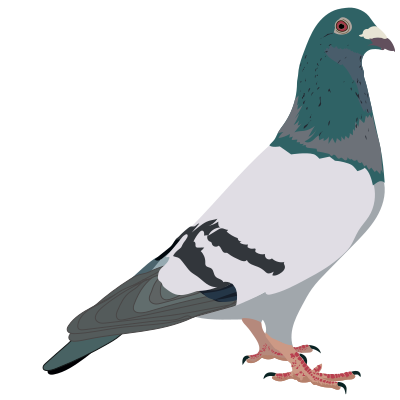
\includegraphics[width=1in]{../cover/pigeon-logo.png}}
\date{}

\begin{document}
\frontmatter
\maketitle

\clearpage
\small
\emph{By Sound Alone}\\
© 2023 Mark Torrey, CC BY-NC-SA (See license at end of book.)

(Final Beta; Version-date: August 15, 2023)

For more information, visit:\\
grannycart.net/by-sound-alone/

uuid: df78bb38-3009-4e40-a4ba-82a73e75a3c4
\clearpage

\mainmatter
\newpage

\hypertarget{preface}{%
\section{Preface}\label{preface}}

You can skip this preface. Go ahead, I don't mind at all. Actually, I
encourage you to. I'd much prefer you dove directly into the story than
have you slog through this first thousand words or so for no other
reason than a sense of duty or a need to complete things. `Entertainment
first' is the rule here!

But if you are among those inclined to wring the most you possibly can
from a book --- or if you've already \emph{read} this book and are back
for a second pass to try to to wring a bit more out of it --- well then
for you I've got this preface in here to maybe shed some light on a few
of the more obscure themes of the book. If you do finish the preface,
you may stand to gain an ever-so-slightly fuller experience when you hit
the book itself. And hey, that's a kind of entertainment too.

The core theme of the book (and, OK, it's not actually obscure in any
way) is an exploration of how humans live with their machines. Today we
have more machines doing things for us than ever before, but the premise
of this book is that there is something special about the human
relationship to \emph{mechanical} machines. This book is about a
particular type of human interaction with machines --- the type that
makes the human a ``mechanic.''

In the latter part of the 19th Century and through most of the 20th
Century, technology changed the world. But the technology of that time
was different than ours. It was rooted in mechanical and electrical
things. In that time, anyone who wanted to understand how a piece of
amazing new technology worked could simply take it apart. Most things
had an intuitive structure --- mechanical solutions based on logical
processes. This is not the same as being \emph{simple}. Many things from
that era were in fact far more complex than today's equivalent devices.
But learning how something worked --- and how to repair it --- only
required a willingness to disassemble (and, following that, a whole lot
of experience doing it). Most parts also had a macroscopic quality. They
worked on a human scale. You could see the parts without magnification,
you could place a part where it belonged with your fingers rather than
any kind of special tool. Today, technology is changing the world again.
But if you take apart a technical object today, all you will find is
vanishingly small components that cannot be repaired, only replaced. And
sometimes even the creators do not understand how they work.

Because of its mechanical underpinnings, that old technology also just
\emph{behaved} more rationally. Even those who had not the faintest
grasp of the fundamentals of how mechanics worked, would learn how their
machine would behave just through the experience of using it. A good
mechanic could tell by \emph{feel} that something was going wrong and
could often guess what particular part was failing, rather than
suffering randomness manifesting itself in the system. People could
depend on their technology to behave intuitively when they used it,
unlike our modern digital-based technology where even experts can be
shocked by what it does and find themselves at a loss to explain why.

This old mechanical technology also came with an aesthetic. The
mechanical nature of it made the stuff dirty, greasy, and grimy. It was
powered by the air-fouling burning of things, kept lubricated by
chemical greases, and cleaned with penetrating toxic solvents. This
aesthetic permeated our culture. The rich found ways to constantly clean
it. The poor and the technology maintainers simply lived in and among
the grime.

Many stories from that mechanical age are often gripping because they
told of average people achieving amazing things with the exciting new
tools available to them. Often those average people made their
extraordinary tools and technologies perform far beyond their original
intended use. To this day there seems to be no end to the delight people
take in stories of electro-mechanical machines. Indeed, we may yet still
be more engaged with electro-mechanical stories than with stories
derived from our modern technology: nearly everyone would rather follow
the building of a custom motorcycle than the latest achievements from a
microchip clean-room. It is even possible that the pleasures of
mechanical things goes much deeper in the mammalian psyche than just
human consciousness --- it has been shown that wild mice in a forest,
given a wheel, will choose to spend their idle time running on that
wheel.

The story told in this book is hung on technologies that anyone could
understand with nothing more than a little armchair-pondering. The world
this story lives in is confined to technology that is \emph{non-magical}
and accessible. Mechanics become the medium for the story. More than
that, I hope the reader who rides along with those who try to live among
those machines can also \emph{feel} how the machines behave, what they
can and cannot do. When this works, it sometimes becomes possible to
leverage the reader's sense of how machines behave to a point where all
the drama can be compacted into nothing more than the movements of a
needle on a dial.

Today's technology has crossed a line into the magical, and there is no
way to put that technology back in the bottle even if we wanted to. But
it is possible in the context of fiction to imagine a world where the
electro-mechanical remained the dominant root of our everyday technology
for far longer than it did. It is possible to imagine that, but for the
geopolitical and economic winds blowing in a slightly different
direction, the commerce and industry of our world could still be carried
out by independent operators driving grease-coated machines steered by
mechanical linkages. Such is this book.

---M. Torrey, July 2023

\begin{center}\rule{0.5\linewidth}{0.5pt}\end{center}

\bigskip

\newpage

\hypertarget{tablemount}{%
\section{1. Tablemount}\label{tablemount}}

The weight of the atmosphere pressed the night down on the ocean. The
air above the black water was pinned under a murky dome of heavy cloud,
held down like some great hunting feline gripping its claws into a dying
songbird. The weight compressed the air to complete stillness,
flattening the water until it was unable to raise more than a barely
perceptible heave, forced up from somewhere deep below its glassy
surface where it still held its hidden reserves of power.

A distant moon --- cast out by the atmosphere and not visible --- dimly
lit the clouds to the color of the charred edges of a coal. The moon
reclined, above and beyond, unable to muster enough warmth to intervene
with the iron grip of the atmospheric pressure. It merely stood by
helpless, feebly attempting to stir the ocean out from under the strong
arm of the atmosphere by the force of tide. It was all it could do to
provide even the coldest, dimmest light. That light filtered down
through layer upon layer of gray cloud until it was so diluted and
refracted that it left the sky only a few shades of black lighter than
the water.

The ocean below was unquestionably black. The blackness had risen up
from the deep. Out beyond the atmosphere rode heavenly bodies that
radiated light and heat, and the thick gasses of the atmosphere carried
some portion of that warmth down to the surface. But in the deep there
is darkness and cold, and the viscous liquid transported that darkness
up to the surface, carried on vast swells of cold. As hard as the
atmosphere might press down, the darkness yielded not at all to the
pressure above.

The boundary where the black water met the pale air stretched from
horizon to horizon along the cupped edge of the dome of cloud in all
directions, without referent or feature. Until a point arose. A
minuscule and meaningless point, like the first push of a needle through
the underside of a new piece of fabric, the workings of which would soon
join the fabric irrevocably and forever to another with hundreds of
interwoven and gradually tightening stitches. The point rose, a long
thin wire extruded up, piercing through the surface. A weak V-shaped
wake trailed behind it in the water marking its course. The tip of the
wire wavered in the thick air, describing great arcane gestures that
were transmitted up its length and amplified from the chaos of forces
afflict acting its still-submerged lower reaches.

The base of the wire emerged, mounted atop a short mast which followed
the wire up through the surface, and soon after accompanied by a series
of a half dozen or so other masts, each adding a new wake behind it. The
line of wakes carved up the black surface behind the path of the masts
with their nested Vs. For a minute they moved alone on the surface, and
the Vs grew longer and longer, stretching out behind in a subtle but
ever-widening trail.

A black oblong pushed through the surface and rose up into the air.
Water streamed across the flat top and down the smooth metal sides of
the oblong. It grew upwards, like a rising column of soot from a
factory, and became a curved vertical wall. It thrust up against the
pressure of the atmosphere with the same manner that seismic forces
raised up a new continent. Water shot out of vents in the side of the
walls, draining out interior voids that had been filled when it was
submerged. The curved wall sprouted up from a giant body at its base,
which now broke through the surface lifting the wall further into the
air above. An enormous flat deck was called into existence in a long
line far before the curved wall of the oblong. The sea water washed back
and forth across the deck, the pressure of the atmosphere finally
yielding to irresistible forces generated from a machine made by humans.
Water ran from the deck, down the curved sides containing huge tanks
that moments before had been filled with water. Now buoyant air
displaced the water, raising the deck upwards. The surface of the black
ocean gave before the breach of this leviathan, and a wake of dull gray
broke out behind it.

At first its movement was nearly silent, other than the sound of the
water running along its sides and the soft crash of the curling wake
left behind. Then it coughed, spat, and from two pipes that opened at
the top of its oblong dorsal fin two arcs of flame burst orange into the
surrounding night, spraying apocalyptic color across the landscape of
pitch. The flames flashed over the reflective blackness of the water and
bounced back from the low clouds, and then died back into the dens from
which they came. They left behind the rolling churn of exploding diesel
and hot air pouring up through the pipes and forcing the shutters open
that normally protected them from the influx of water.

The engines of the machine revved up, and then maintained a loud high
pitch, generating the energy to drive it forward through controlled and
contained combustion trailed by blowing heat. The surfaced submarine
accelerated, reached, and maintained an unvarying speed.

Set into the top of the dorsal fin was a recessed platform. At the
bottom of the platform was a black well of a hole that led further down
into the fin.

At the bottom of this well, a rusty wheel turned and creaked. It was
followed by a crescent moon of red light that split the black well
bottom and widened into a perfect circle as a hatch lifted open. The
shadow of a small figure climbed through it and up a short metal ladder
to stand upright on the recessed deck platform. This smaller first
shadow was followed by another much larger shadow. Both figures looked
around at the darkness, pitch except the red glow rising up dimly from
below their feet. They leaned forward and rested against the fairing.
The smaller figure made some gestures to the darkness, and a match light
glowed against the end of a stubby roll of tobacco.

The glowing coal swept a thin line in front of them as an arm opened to
the darkness. The figure next to her, dwarfing her in size, just nodded.
There was no need to describe the all-consuming blackness aloud.

The giant figure, slowly pulled his fingers through his thick beard.
``Perfect night for a surface run.''

``Perfect night for contemplating your doom, Hemi,'' said the smaller
figure.

``If darkness stirs up feelings of doom, then wear your doom like a
blanket.''

``It's probably best if you keep your imaginative comparisons to
yourself. After all a blanket is for warmth --- our doom is unlikely to
be very warm.''

``Perhaps so.'' Hemi paused breathing in the dense smell of the burning
tobacco; there was no reason to rush anything this night. ``The usual
plan for tonight then?''

``Same as every other fucking night. Charge up the batteries --- run on
the surface till the light cracks the sky, and then we'll disappear back
where we came from. Make sure your keep those pissants at the controls
awake though.''

Hemi put one huge hand on her shoulder and turned to climb down through
the hatch. She pulled on her cigarillo and the coal at the tip glowed in
the darkness. Her doom would probably eventually be a doom of freezing
water, she knew that, but at least tonight it was warm enough to be out
in the open, up on the top of her boat. The blackness lay on it, and she
did indeed find some comfort in it: nobody could see them. If she
controlled all the levers of the universe, her vessel would never be
seen.

\bigskip

Captain Sylvia Percy stayed on the bridge of the her submarine's sail
for hours, smoking her way through one cigarillo after another and
watching the empty nothingness go by while her thoughts spiraled outward
without direction. For a long time she was surrounded by an environment
disturbingly deprived of sensory input. The diesel engines were loud
enough, but unvarying. So too the vibration that the engines sent up
through the steel-grated deck to shake the worn rubber of her boot soles
without change in frequency or amplitude. The blackness around her was
limitless, though the boat pushed relentlessly forward. It occurred to
Percy that when her boat, the \emph{Prospect} was submerged, this is
what it must be like outside: featureless dark. It felt like she had
loosed the bonds of her corporal body and had floated beyond it, so she
could experience what her boat was like when it was pushing through the
icy blackness of an alien world where the pressure would collapse any
body that had evolved for comfort on the surface into a sickening
unrecognizable mush of hemoglobin and fats.

As with many things that seem interminable, the slow but persistent
forward motion eventually forced the dome of clouds to relent. The
submarine pushed through to crawl out under a sky of stars and a weak,
low moon. Captain Percy could see her hand holding her latest cigarillo
now, and the long shadow of the \emph{Prospect} stretching out ahead,
parting the waters to allow her to pass as she rode astride this beast
of hers. This was a pure and rare pleasure on a submarine where she
spent the vast majority of her time in a steel tube staring at the same
set of dials with few opportunities to focus her eyes on anything beyond
a meter in front of her.

Captain Percy knew her boat well. She had spent enough time with it to
have internalized its movements. She almost always knew what the boat
was doing just by the feeling of it --- the angle of the deck, the
vibrations of the engines or the electric motors, the subtle changes to
the pressure of the air. Even at depth --- when the hull and struts of
the boat groaned under the weight of the water above --- to her the
sounds of the boat under pressure felt like the normal sounds of a huge
human taking a great weight on its shoulders. The only time she ever
worried was when the \emph{Prospect} conveyed sounds or motions, or some
other input, that she could not recognize. She had been through so much
with this boat that it was only when it did something new that she got
scared.

It was when the \emph{Prospect} had moved fully out from under the
clouds, and everything was lit to a dull blue by the moon, that she felt
something new. A collection of haptic feedback to her senses made panic
rise in her chest. The boat shuddered, as if the cold water it swam
through all these years had finally chilled its core.

Captain Percy was thrown violently against the fairing.

She immediately dropped to her knees on the deck of the bridge, her
short fingers pushed through the gaps in the steel grating and gripped.
She stuck her head over the hatch hole and looked down to see Hemi's
large face looking up at her from a couple of deck-heights below.

``I don't know!'' He yelled before she could ask. She could hear him
haranguing the deck crew to kill the diesel engines and reverse the
propellers.

The bow of the \emph{Prospect} had come to a dead stop, but the stern
still had forward motion. Captain Percy could feel the whole boat
turning unnaturally around its center axis, like the experiment of some
precocious child: a magnetized pin through a cork floating in a bowl of
water pulled around by the invisible forces of a planetary aura.

The deck under her began to lean to the starboard side. Captain Percy
propped one foot against the inside of the bridge well wall. The boat
listed sickeningly. She got to her feet, still braced against the angle
of the boat. The pads of her fingers gripped the sharp rusted edges of
the fairing, and she peered out over it into the night, scanning for
what they had hit. The water to the starboard side remained black and
calm, though not quite as glassy as it had been earlier in the night.
They were far from shore, in fairly well-charted though
little-trafficked waters. The \emph{Prospect} had clearly run into
something at full surface speed, but there should have been nothing to
hit here.

For a few moments the boat hung at an angle with no motion and all
potential. And then it began to right itself, tilting slowly back
towards the port side. As the edge of the fairing came down, Captain
Percy could see more of the sea off to port, and there appeared the
shadowed silhouette of another submarine.

The bow of the other boat rose up out of the water first, revealing one
of the rarest things seen on a modern submarine: a distinguishing
feature. The bow had a jagged point that swept back in long sharp blades
to merge incongruously into the soft curves of the submarine's hull.
Curved teeth sprouted all along the blades, and those had been
reinforced with welded crossbars in many more places that could possibly
be necessary. A medieval-looking device intended for ramming ships.
Captain Percy had never seen anything like it. It must be both a noisy
and inefficient thing for a sub to push through the water ahead of it.
Efficiency and quiet were normally the top priorities for a submarine's
design.

Behind the snags of the bow ram followed the smoothly swelling curve of
a black military submarine. It came up from the surface with water
streaming slickly down its sides. The sail rose above with dive planes
mounted to it, sticking out like small wings and set at an angle to
raise the sub quickly. When the stern finally broke the surface, it was
mere meters away from Percy, its swirling wake washing white up the
against the side of the \emph{Prospect}.

``Might be our fucking doom a lot sooner than we anticipated,'' Percy
said to herself as she climbed down through the hatch and the red
crescent of light waned out of existence behind her.

\bigskip

She hung on the metal rungs of the ladder just under the hatch set in
the ceiling of the cramped control room of her submarine, and with one
hand quickly screwed shut the squeaking wheel of the hatch seal before
dropping to the deck. Hemi looked down at her through his small-framed
spectacles.

``Down.'' She gave the one-word command as she pushed the button on the
wall that activated the dive alarm.

``Give me full speed forward,'' said Hemi. He put one large hand on each
of the shoulders of the two men who sat at the controls of the sub and
instructed them to dive the boat. One of these men was a stick-figure of
a man who went by moniker Bastian. The other, ``Handsome'' Gregory, had
a meaty square forehead that looked like a miniaturized version of his
meaty square torso. Of the two of them, only Gregory looked like he
belonged on a submarine.

Diving the sub required delicacy even in the calmest circumstances. Now
Hemi and the two men at the controls carefully timed their movements.
Their eyes scanned continually over the wall of dials, gauges, switches
and valves in front of them that reflected back the red glow of the
night lighting. This wall at the front of the control room told them the
\emph{Prospect's} angle, depth, speed, systems settings, battery charge
--- the whole picture of the boat's orientation and movement. Indeed,
this wall plus some of the panels situated to their right and left were
the \emph{only} way to know the status of the boat while it was
submerged.

Gregory and Bastian made adjustments according to Hemi's instructions,
choosing carefully which of the dozens of valves mounted on the control
panels in front and around them to open or close, or which switches to
flip on or off. The submarine let out a long exhale of breath: the air
that had held it aloft on the surface being pressed out by an onrush of
water from below into the flooding tanks.

``Flood the express dive tank,'' said Hemi in a low voice since the tiny
space of the control room did at least have the benefit of making it
easy to hear one another.

``Right, Boss.'' Bastian reached up and opened a valve and water thrust
through thick old pipes into the deepest parts of the bow of the boat.
The forward part of the boat pitched steeply downwards in response.
Captain Percy reached to grab cracked leather loops that hung overhead.
She angled her feet against the incline and her eyes followed the needle
of the depth gauge.

The ship-to-ship radio above Captain Percy's head lit up. From the
radio's speaker a recorded voice began blatting a warning that they were
violating the territorial waters of someone they had never heard of; who
were authorized by a series of treaties with titles that became acronyms
that became words that contributed to further acronyms. The recording
concluded by ordering all submerged submarines to surface and prepare to
be boarded.

Percy reached forward and punched the mute button on the radio.

``Only on the surface do these fucking territories and treaties
matter,'' said Captain Percy.

Hemi nodded.

``What the fuck happened up there?'' Gregory asked, his eyes never
leaving the wall of dials and gauges in front of him.

``We were hit. Sub with a big ugly ram mounted on the front of it.
Totally fucking insane thing for a submarine to have,'' said Percy.

``Possibly some specialty-built Authority enforcer boat.'' Hemi sounded
unconvinced by his own hypothesis.

There was barely enough space in the control room for four people. They
were all breathing each other's air. Their breath condensed on the cold
glass faces of the dials and gauges. Hemi took a rag from a hook and
reached in front of the two seated men to fastidiously wipe each of the
little round windows clean.

``100 meters,'' said Gregory.

``OK. Level us off,'' said Hemi. Gregory and Bastian spun closed some of
the trim tank valves and rolled the dive planes back to align with the
long access of the sub. The angle of the boat slowly eased upwards
bringing the deck beneath their feet level.

Hemi stood staring at the dials in front of Bastian and Gregory, his
massive arms crossed in the rough wool of his tightly-fitted tweed suit
jacket. He tapped the thick fingers of one hand against the leather
elbow patches while his other hand stroked his wiry black beard. He gave
a few more instructions and got the boat moving slowly and silently,
running level at depth. The idea was to sneak quietly away --- the most
routine tactic of all submarines. But the routineness of it did not
reduce the sense that they were playing the role of prey.

Captain Percy pulled a new cigarillo from the crinkled pack in her
pocket and lit it. She sucked at it, and then ashed into a tin cup
wedged between the pipes running along the wall that smelled of her
stale coffee from three hours earlier.

Being underwater meant they had to run on batteries. The diesel engines
the submarine used while surfaced generated power that drove the
propellers and charged the batteries. But those engines breathed far
more air than humans, and so could not be used underwater. Running on
batteries with just the electric motors driving the props made the boat
nearly silent. The electric motors produced a hum that was audible
inside the boat (Percy always thought it to be a pleasant, reassuring
hum), but was barely detectable by another vessel. Eventually the
batteries would run out though, and they would have to get back up on
the surface to recharge the batteries with the diesels.

But Captain Percy's intuition was plaguing her again. ``Something isn't
right,'' she said aloud to no one in particular. Like when they had been
rammed, the \emph{Prospect} was again doing something new that she had
not felt before. But this time it was not a quick jolt, like the ramming
had been. It was something so subtle, such a delicate change in the
motion of the boat, that the others did not feel it at all. Actually,
she was not even sure it was a change in the \emph{motion} of the boat.
Maybe it was something that was not making sense in the information she
was getting from the gauges.

There was no single instrument that reported anything amiss. But then no
single instrument on a submarine described the total status of the boat.
All the instruments had to be taken together, internalized, and combined
with what one physically felt the boat doing. Percy would typically be
holding the depth in her head, while also taking into account the dive
plane angle, the speed, and the overall feeling of the boat. Normally
this happened instinctively. She processed it all automatically, and she
could just \emph{know} what her boat was doing from a quick glance at
the wall of dials combined with what her senses told her and dead
reckoning from the accelerations she had experienced.

This feeling of internalizing what her boat was doing --- something she
did continually, to the point where it felt like the boat was part of
her body --- felt inexplicably broken at the moment.

Her eyes scanned back and forth across the dials, but the information
did not come together. There was no way to make sense of the dials. In
this steel tube with no windows, perhaps for the first time ever, she
felt blind.

``Hemi\ldots{} what the fuck is going on\ldots?''

``I do not know\ldots{} we are within normal tolerances\ldots{}
though\ldots{}'' He reached past Gregory and turned the rudder. The boat
came along, slowly. ``Sluggish?''

``I need to go look my girl over. Let me know on the PA if something
happens.''

Hemi nodded and Captain Percy slipped down the ladder to the deck below.
She stepped to the front of the navigation and sonar compartment and
climbed down a steel ladder to the middle deck of the boat. This was
crew quarters. The \emph{Prospect's} third deck-crew member, Owen
Smalls, was off watch and snoring in his rack behind one of the
moth-eaten old bed curtains. She continued through a hatch at the rear
end of crew quarters and down another steel ladder to the lowest of the
three main decks. If there were something physically wrong with her
boat, this deck was the most likely place to figure out what it was.

She flipped on the lights. There was no red night lighting rigged down
here, it was just bare white bulbs behind protective steel cages. The
lights stretched off in a line on the ceiling, forward and aft of her.
This particular lower-deck compartment was entirely full of batteries,
strung together with a web of black cables as thick as her finger. The
cables were grouped together with wire ties and slung along the racks in
heavy bundles. The batteries were bolted with rusting steel straps to
row upon row of steel shelves.

The deck was steel grating. She got to her knees. The steel grating
pushing through her the knees of her brown leather overalls that were
cracked at the joints where they bent. She put her fingers through the
grating and lifted it up and put it aside. She reached her hand down and
felt the raw steel of the pressure hull. It was cold, damp, and greasy,
but that was normal. She replaced the grate and went on to the next
compartment forward.

More batteries here, though fewer. They lined the walls, but not as
deeply as the previous compartment because there were trim tanks on
either side inside the pressure hull here. She checked below the grating
again, but here too everything had the normal amount of greasy dryness.
She passed forward from that compartment through a hatch into the main
cargo hold.

The main cargo hold was one giant void occupying most of the front half
of the boat. More than thirty meters long, and almost ten meters wide.
The air was still and stale. It smelled of rust and petroleum, grease
and oils. The overhead bare bulbs had a harsh jaundiced yellow color.
The hold was mostly empty --- they had been coming from their last cargo
drop-off and were heading towards the depots in the north with the
intention of getting another shipping run job. A few wooden crates,
stippled green and black with mold, were stacked up along the sides. In
another nook was stashed a couple of welding rigs wrapped with chain and
some bins of scrap metal piled up against a greasy grill used for
cooking on deck. It had always bothered Captain Percy that they could
not find a more considered place to stash these sundries than the cargo
hold.

She walked along the center line of the space --- the spine of the boat
--- listening carefully. It seemed to her there was something wrong with
the sound of her footsteps on the metal grating. As she neared the front
of the compartment, she realized it was not the quality of the sound of
her footsteps, it was that she could hear water trickling faintly. She
knelt down and pulled up the grating. There was a pond of oily black
water just under the deck level. In it swam a small school of old
cigarette butts. Little ripples formed from resonance with the hum of
the electric motors, their vibrations passing up the hull and encoding
themselves on the scum of the surface here.

There should not be this much water. Percy now knew exactly what was
wrong with her boat: the ramming had cracked the pressure hull, and the
\emph{Prospect's} cargo hold was filling slowly with water.

\bigskip

``Keep this depth, and course, I will be down at sonar listening for
that sub.'' Hemi climbed down from the cramped control room to the
compartment below. If he turned and leaned back from the sonar station,
he could almost see up into the control room just behind and above him
and could still tell the men at the controls of the boat what he wanted
them to do. Likewise, Gregory and Bastian could still give him reports
on the \emph{Prospect's} status, albeit with a little more emphasis
thrown into their voices so they carried below to Hemi.

Hemi did not bother sitting down at the sonar station. Instead, he stood
behind the empty sonar operator's chair and slipped the headphones with
the worn ear-pads onto his head. He covered one ear and left the other
free. He spun the control wheel for the sonar around slowly, listening
for human sounds out in the malevolent underwater darkness of the ocean.
There was nothing but silence.

``Hemi,'' Gregory called down through the hatch, ``I'm having trouble
keeping the boat level. I find I keep having to give it more and more
upward dive plane angle just to keep from gaining depth.''

``Let me come up and play with the trim tanks.'' Hemi climbed the ladder
back to the control room. He stood at the trim tank controls next to
Gregory and the thick pads of his fingers spun one small steel
valve-control wheel, then the next. Each was accompanied by the sound of
water pushing through pipes, flowing from one end of the boat to the
other. ``How's that?'' asked Hemi after a few minutes of adjustments.

``Better, but still quite a bit more dive plane angle that I would
expect just to keep the boat level,'' said Gregory.

Hemi did not say out loud what he was thinking: they were sinking.

\bigskip

``Sweet fucking hell,'' Percy said to herself. ``Sweet fucking hell!''
she repeated at a yell. She ran up the length of the cargo hold, her
clomping boot steps echoing in the empty space. Back in the battery
compartments, she pulled the heavy watertight bulkhead closed behind her
with a loud metal-on-metal sound, and turned the wheel to seal the cargo
hold. It took all her strength; the screw-wheel seals in this part of
the sub were rarely used, and they were planting themselves ever more
firmly into a rusted stasis as time passed.

She climbed up a deck, and passed out from the back of crew quarters,
through the galley, and into the engine room. The only sound there was
the throb of the electric motors spinning in the next compartment back,
and a randomized clanking of tools from the deck below. She leaned over
the open hatch to the lower engine room.

``Chips! Chips, come over here.''

The clanking sound stopped and the face of the \emph{Prospect's}
engineer appeared below the opening a moment later, peering up at her.
Chips hands were black with grease that had also created a grimy patch
on the leather apron she wore. In her hands, as if she had been
butchering some small game animal for dinner, she held the shell of a
deconstructed piece of machinery about the size of a baseball.

Percy recalled that Chips' real name was Irene something-or-other, but
Hemi had stuck her with the nickname ``Chips'' when she had signed on.
According to Hemi, ``Chips'' was the traditional nickname for a ship's
carpenter going back to antiquity. And even though there was little
carpentry to be done on a submarine, the ship's carpenter was generally
responsible for any number of random jobs that needed to be done but
were not already assigned to the deck crew. When she had first come
aboard, Hemi had such a list of things that needed doing on the
\emph{Prospect} that he felt the name was appropriate to the new
position. Also, he had always wanted a ``Chips'' on the boat --- he was
a fan of the classics.

``What the fuck is going on Percy?'' Chips asked.

``There's a leak.'' These were words no submariner ever wanted to hear.
But Chips had fixed leaks before. It was the answer to the next question
that Captain Percy was loath to give her.

``I was wondering when one of you assholes would make their way down
here and tell me that the fuck's with all the fucked motions of the
boat. Where are we leaking?''

``\ldots In the cargo hold.''

``And it's fuckin' bad, eh?''

``Ah, pretty\ldots{} fucking bad. An Authority sub rammed us on the
surface, apparently split open the pressure hull.''

``Split it\ldots{} in the fucking cargo hold you said? So then we're
fuckin' fucked, eh? Haven't I always fucking said that cargo hold's too
fucking big, and it should have bulkheads? The fucking boat won't float
if it's flooded; eh, Capt' Percy? That's what you're fuckin' thinking
right now, ain't it? You probably didn't want to even fucking tell me
because you know that we're fuckin' fucked!'' She threw her piece of
machinery at the wall where the loosely-held assembly separated and sent
small parts flying far into the black corners of the lower engine room.

``For fuck's sake Chips, yes we're fucked, but we're not \emph{fuckin'}
fucked, not yet\ldots{} I need you to take one of the guys, go in there,
and see if you can stop it and patch it so we don't get to the point
where we \emph{are} fuckin' fucked. Right?''

``Ah, fuck ya Capt'.'' Chips started climbing up the ladder towards
Percy without looking at her.

``You and your attitude! Listen to me,'' Percy held her arm, ``good or
bad, I need regular reports. Get Owen up and get him helping you.''

Chips wrenched her arm free. ``A- fuckin'- OK.'' She gave Percy a mock
salute and pushed past to enter the upper engine room.

Captain Percy left Chips digging out hull patch kits from engineering
storage compartments and returned to the control room.

Gregory's square head came around and his beady eyes caught hers as her
head popped up through the hatch in the floor of the control room.
``Wish we had something to shoot at those fuckers who rammed us.''

``Someday, you handsome young man, I'll refit the \emph{Prospect} as the
first merchant sub with a torpedo tube --- just for you. Until then, our
defense is the same as any prey animal: run and hide.''

``If you are back in the control room for the moment,'' said Hemi, ``I
will go down to sonar to work on tracking that sub with the ram's
location. And how is our boat, holding up?''

``We're sinking. I put Chips on it.''

``If she can patch the boat with expletives and downright
pissed-offedness, we will be in good hands,'' said Bastian, without
turning around.

Captain Percy stepped off the control room ladder and yielded it to Hemi
on his way down. She addressed Gregory and Bastian, sitting in front of
her in their control chairs. ``What's the state of my ship boys?''

``Apparently we're fucking sinking,'' Gregory answered.

``Fucking apparently\ldots{}'' she agreed. She scanned the gauges. There
was nothing immediate in their impending doom. It was written instead in
subtle ways, spread across the dials, and only when the readings of the
dials were taken altogether. The dive plane angle was too steep for the
amount of forward drive they were giving the boat. The trim tanks too
light. The depth deeper than she wanted to be.

``Since that sub is going to know where we are anyway, you might as well
crank the bilge pumps up to maximum power. Making a bunch of noise is
better than sinking.''

Gregory flipped some switches and another frequency of vibration was
added to the regular background hum from the motors propelling the boat.

Percy lit a cigarillo from the rapidly-depleting pack in her pocket and
smoked it down, letting her mind sink into the ever-present hum of the
machines that swamped her environment and ruminating on the gauges.
``How's she handling generally?''

``The boat just doesn't seem fucking normal Cap. It doesn't respond how
I want it to,'' said Bastian.

``Here, let me try the rudder.'' She reached over him and turned the
wheel hard over. The \emph{Prospect} came about slowly but surely,
leaning over slightly, as she should. But after a short delay the whole
boat took on a sudden heavy list. Percy counter-steered and brought the
\emph{Prospect} back to the course they had been on.

``See? That doesn't seem quite fuckin' OK to me,'' said Bastian.

Captain Percy knew it was worse than that. The sharp list after the
delay was the weight of the slack water in the bilge pouring over to one
side of the boat and dragging the rest of the boat over with the weight
of its movement.

\bigskip

A short while later, Percy had finished her cigarillo. ``I\ldots{} need
to go check on Chips.'' She slid down the ladder from the control room,
passed Hemi concentrating on listening to the headphones at the sonar
station, and continued forward until she got to the steep metal stairs
down into the cargo hold.

Chips and Owen were working at the far end where they had rigged bright
work lamps. Owen was dragging one end of a fat gray, grimy hose for an
old mobile bilge pump from the pool of black water in the bow up the
middle of the cargo hold towards the fixture set in the wall where a
hose could be fed to the trim tanks. Chips had a whole set of the deck
grates out and stacked up to expose the pond of scummy black water under
them. She was wearing thick rubber waders and standing directly on the
inside of the pressure hull in the fetid water. The water had pooled up
above the grating level and was almost to Chips' chest --- a distressing
sight that was tempered in Percy's mind by the knowledge that Chips was
not a tall woman. Chips had heavy rubber welding gloves on and a mask so
she could see what she was doing under the water. Above the swim mask
she wore another dark-lensed mask for welding that could flipped up or
down as required for doing the work.

As Percy was walking down the cargo hold, Chips' head was disappearing
under the surface. She stood on the grating above Chips, watching. The
welding rig next to her revved up with a hiss and a groan, and a stream
of bubbles and flashing blue light pierced through the turbid water.
When Chips lifted her head for air, water ran down her mask in rivulets,
and drained in a greasy gray stream from her matted hair. Percy asked
her for her report.

``Fuck you, ya dominating fuckin' cow. This is delicate fuckin' work
here and you're up on there in the control room sloshing the whole
fuckin' boat back and forth. And it needs fucking time. The hull's got
hundreds of tiny cracks. It's split open the way ya might break off a
piece of cheese --- tiny cracks all the fuckin' way along. If it were
one big crack it would be much fucking simpler. Hand me that fuckin'
patch piece by your feet.''

Captain Percy spat, and her spit tasted oily and gritty. She handed
Chips the flat piece of sheet steel, which was coated with a slippery
residue. Chips held it against the side of the hull and pulled a hammer
from a loop on her waders. She hammered it against the side of the hull
with heavy, ringing smacks, shaping it to the interior curve of the
boat. Percy was sure she could hear the ring of the hammer traveling
along the steel pressure hull all the way to the stern. She could
imagine the sound going out into the water, which felt like a violation
to her basic instinct to always keep her submarine quiet. Practically
though, it hardly mattered, since those who pursued them would already
know their location anyway.

Chips took her now appropriately curved piece of patch steel and
submerged into the filth again.

Percy watched her work for a quarter of an hour or so. Even in that
short time she could see the line of water on the hull had visibly
risen, crawling its way up the grated deck, slowly consuming her boat.
Owen came back and started up the rattly old bilge pump, and with a
whine and a rush of water that gave a serpentine life to its hose, it
began a losing battle to take back some of the boat from the maw of the
beast consuming it.

It was hopeless though. The water level in the cargo hold was rising
more slowly now that Chips had some patches in place, but still rose
relentlessly. By the time Chips next brought her head above water,
Captain Percy had made a decision she did not want to make. ``Keep
working,'' she told Chips, ``I'm going to blow the tanks and bring us up
to the surface.''

``Fuckin' smartest thing ya said yet this fuckin' day. This course we're
pursuin' right now is on a fuckin' trackway to the gates of fucking
Hell.''

\bigskip

Percy climbed back up the stairs to the third deck, moving towards the
control room. As she passed Hemi at the sonar station she told him she
wanted to blow the tanks. He nodded, as if he had been expecting it.
``What about the sub following us?'' he asked.

``We've reached the point where we're better off with them up there than
fucking sinking down here,'' she replied. ``I'll be in the control room
to keep her stable during the rise. I want you to open the tank blow
valves.''

``OK,'' said Hemi, taking off the headset as he stood up from the sonar
station.

Blowing the tanks was an emergency maneuver. It meant opening the valves
that would allow air to flow through the convoluted paths of the old
pipes of the ship and push into the tops of the main ballast tanks. The
air forced in the top of the tanks would push water out the bottom. When
enough water was forced out, the huge bubbles of damp, greasy air held
at her sides would rapidly raise the submarine up to the surface, like a
child being gripped by the armpits and tossed upwards. Fully blowing out
the tanks was only ever done in emergencies and drills, and drills were
few and far between on a cargo sub like the \emph{Prospect}. It put
stresses on the old boat, stresses it was designed to handle --- when it
was built more than 20 years before.

The emergency blow station was at the back of the sonar \& navigation
compartment, where the equipment made a subtle shift from the electrical
to the mechanical. It consisted of a number of pipes mounted up against
the wall of the compartment. The pipes ran forward and aft from the blow
station, off into the many deep, complicated parts of the ship that
controlled buoyancy. The pipes had the diameters of large soup cans.
They had been re-painted many times, giving them a thick smoothed-over
texture, except where the paint had chipped off with flecks of rust.
They were stacked up, more than a dozen. Some passed through on their
way up to the tank control panel in the control room. Others routed
through this compartment simply for the convenience of the engineering
of the boat.

Four of the thickest pipes led from the high-pressure air tanks to the
main ballast tanks. There were large valves set in-line in those pipes
that could be opened or closed by turning a heavy hexagonal nut. Turning
the nut required a large wrench.

Hemi stood in front of the pipes and opened a long metal toolbox bolted
to the wall between them. From it he took a wrench as long as a forearm
--- not Hemi's forearm, but the forearm of an average-sized human. The
wrench was wrapped in a pilled rag that had been dyed a bland gray color
from the decades of grease worked permanently into the fibers. He fitted
the end of the wrench over one of the heavy nuts controlling the valves
and wrapped the rag around the end of the wrench where he gripped it.

``I am ready to blow the tanks,'' he said with some emphasis, aiming
this statement up to the control room hatch forward and above him. ``At
your service, Sylvia.''

There was a pause while Captain Percy worked with Gregory to get the
trim tanks and control surfaces of the boat configured the particular
way she wanted them for this hazardous maneuver. Then: ``OK Hemi, open
the ballast blow valves!''

Hemi pushed his fat thumb against the cracked black rubber coating of
the emergency blow alarm button set in an electrical box between the
pipes. A klaxon wailed into the deepest corners of the \emph{Prospect}.
Then he turned the wrench until it was horizontal, aligning it with the
run of the pipe. He repeated this action with the sister pipe running
just above it that would blow the aft ballast tanks. Accompanying each
turn was a squeal and a hiss, and then a rush of air moving through the
pipe, like the howl of the hunting hounds of an ancient god riding
across the sky.

The expanding air in the pipes forced their temperature to drop. Their
surfaces were instantaneously coated in condensate, which froze and
sublimated to vapor, rising up and away from the pipes like two long
otherworldly fingers passing through the compartment and gripping the
ship. From where Hemi stood, the air in the pipes felt like the shot of
a canon moving past him, leaving a trail of smoke marking its path. He
had the sense of it pushing into every corner of the ship, like blood
pumped into the furthest capillaries of a body. The flushing sound of
the water pressed out into the sea passed through the ship, and the very
mass of the ship itself shifted under the force of it.

``Take us up guys. Set the dive planes, and blow any trim tanks you
haven't yet.'' Gregory and Bastian turned the control wheels. But within
seconds Percy again felt her boat moving distressingly like a wounded
animal. The stern was rising faster than the bow. The angle of the deck
under her feet was leaning in the wrong direction.

``What is going wrong?'' she shouted at Gregory. Her eyes scanned
rapidly across the instruments. ``Trim!'' She started spinning open
valves on the tank control panel, trying desperately to get more air
into the bow and level the boat. Gregory's arms were bulging with tensed
muscles as he his hands gripped the dive-plane control wheel, battling
to angle the bow upwards.

A hazard light lit on the tank status panel accompanied by a foul
buzzer. ``Hemi!'' Percy shouted down through the hatch. ``The forward
tanks didn't blow!''

``The valve is wide open Sylvia,'' Hemi said, looking at the indicator
etched on the nut to double-check his work. ``The ramming must have
pinched closed the high-pressure pipes to the forward ballast tanks.''

The stern slowed its ascent. The \emph{Prospect} hung in the water, the
bow pitched downwards. ``We're no longer rising,'' said Bastian, looking
at the depth gauge.

Hemi stepped under the hatch up to the control room and looked up at
Percy through the small circles of his glasses. With his height, his
face was only a few finger-widths from the hatch opening. ``Sylvia,'' he
said, ``I think we need to start thinking about more drastic measures to
get us back on the surface.''

\bigskip

``The fuel oil ballast?'' Percy asked Hemi. Though he could mean nothing
else.

``Yes, I think we should dump the diesel. Even if we get to the surface,
we could lose the boat if the cargo hold keeps flooding and we can not
figure out how to empty it. That is a bigger risk than not having enough
fuel oil to get to a port --- if we do manage to keep the boat on the
surface.''

Captain Percy considered. But sometimes considerations are meaningless.
They had passed the point of developing a strategy to evade their
pursuers. For a submarine captain, the situation she now faced was was
reduced to a single factor: get to the surface at any cost. Knowing
that, the decision to blow out the fuel ballast tanks --- to dump all
their diesel fuel in the ocean --- did not require any time to weigh
options.

``OK Hemi. Come up here. Keep her under control. I'll blow the fuel
ballast myself.''

There were in fact two long thin toolboxes bolted to the wall at the
emergency blow station. One had the main ballast tank blow wrench, which
Hemi had already used. The second toolbox was padlocked. It contained
the fuel ballast blow wrench. Just like the main ballast, the fuel oil
tanks could be blown out with high pressure air as well. The difference
being that blowing the fuel out of the boat might give them an emergency
pocket of air to lift them to the surface, but it left the boat with no
fuel --- stranded and unable to maneuver.

Captain Percy was the only person who carried the key to this second
toolbox, to ensure the fuel oil tanks could never be blown accidentally.
She unlocked the toolbox and withdrew another wrapped wrench the same
length as the tank blow wrench. But this one had a special 5-sided
socket that would only fit the nut to open the air line into the fuel
ballast tanks --- the fuel ballast could not be blown out with a normal
hexagonal wrench.

She pushed the emergency blow alarm button again and with the klaxon
whining fit the wrench onto one one of the special nuts controlling the
valve in the air pipe. Percy was pretty sure these valves had never been
turned before, not even in a drill. They had been painted over many
times during the decades the \emph{Prospect} had been operating. She put
all of her weight onto the end of the lever and let out a long groan,
but could not budge it. She reached for a spare length of pipe that lay
all but forgotten on top of one of the high-pressure pipes against the
wall and slipped it over the handle of the wrench to extend the length
and get some more leverage.

The nut slowly turned under all her weight pulling on the end of the
extended lever. One-quarter turn to the stop at the open position.

Another rush of high pressure air pushed its tendrils through the ship.
Their precious fuel oil --- the only way to escape the lost emptiness of
the ocean and return to port --- was thrown away from them, out into the
dark waters under the ocean. She repeated the process for the nut that
controlled the compressed air into the aft fuel ballast tanks.

Percy could feel the \emph{Prospect} respond immediately. The angled
deck under her feet leveled off, and the bow came up. She climbed to the
control room, cramped again with its full complement of three people and
one giant.

``Now\ldots{} now are we rising?'' Percy asked after a few minutes. But
she was looking at the same gauges as everyone else. She could read them
as well as anyone else.

``We're\ldots{} holding,'' Gregory reported tentatively.

Hemi made a few adjustments on the tank trim control panel, and managed
to get the \emph{Prospect} level in the water, but could not get the
depth gauge to move. They sat more than 90 meters down from the surface.

Hemi gave his pragmatic analysis: ``the fuel ballast tanks just are not
big enough to overcome half our forward main ballast being flooded.''

Percy scanned her eyes back and forth over the gauges, dials, and the
settings of the switches looking for something, anything, that could
move her boat upward. She pulled a rag from a hook on the wall and
reached over Bastian to wipe at the dials. Then she smashed the meaty
part of her hand against the wall next to the primary depth gauge,
``rise you bitch!''

``Even if we escape from this pit down here, there's hunters waiting for
us up there,'' Gregory said quietly.

``They would have heard our emergency blow. They can see we are not
surfacing. With any luck, they will believe we are sinking,'' said Hemi.

``We \emph{are} sinking, aren't we?'' said Bastian, ``small fucking
comfort that they know it too.''

Owen, the youngest of the crew, stuck his head up through the hatch
though remained standing on the ladder to the control room. ``Captain
Percy, Chips wants me to tell you that all the movement of the boat has
split the cracks in the hull wider. The flooding in the cargo hold is
getting worse. No, wait, she said to tell you this part exactly: `the
fucking cargo hold of your shitty tub is flooding like a damned bitch in
her first season of heat' \ldots was what she said.''

``Her words exactly huh?''

``Under the dark part of the pit are the poison spikes,'' said Gregory.

Owen looked at Gregory with a specific question on his face, but asked a
different one. ``Can't we surface Captain?''

``Go back and help Chips. Do anything she asks of you. Get the cargo
hold patched and the flooding stopped.''

``Alrighty.'' Owen's head disappeared back down below.

\bigskip

Captain Percy was running out of ideas. It was easy to make the decision
to get to the surface at any cost while there still remained some levers
to pull and options to choose between. But now nothing remained that she
could think of that could move them upwards.

She cleared her mind. The surface was less than 100 meters away ---
there were people who could throw a ball that distance. The surface was
not her natural environment anyway. Up there was war, borderlines,
treaties, enforcers and Authorities. Up there was conflict, nations, and
bureaucracy. Under the dark water was where she belonged. Where she
could steer her boat in whatever direction she chose, free to go where
she liked, when she liked. This was a virtue of being able to move along
the Z axis --- something only available to submarines. It provided an
exponentially larger amount of room to maneuver. Still, she had no
desire to die down here. And no matter how safe and free she felt
underwater, there was always that yawning gulf underneath. A dark, cold,
bottomless chasm. Once you go \emph{too} far under, you go under
forever. She enjoyed her freedom, but she did not want to wallow in its
icy depths.

She put the idea of the surface aside. What if she did look under the
dark water instead of up toward the surface light? What was down there
in the abyss? What if they could find safety in the deep?

``Hemi, how far down is the bottom where we are now?''

``1000 meters, give or take. Essentially bottomless.''

``Hmm.'' She slipped down the ladder from the control room and stepped
forward to the navigation table located just behind the sonar operator's
station.

The navigation station sat on top of a stack of flat files which held
charts that were not of immediate use. Behind the flat files, rolls of
charts that were more commonly used were stacked between upright stakes.
When they had the white lights on, the charts showed their age, yellowed
and flaking at the edges.

Hemi had the \emph{Prospect's} current position marked with a grease
pencil on a glass sheet laying over the chart that showed the region of
the ocean they were moving through. The black smudges trailed up away
from the shoreline they had left days before. They were in the middle of
the ocean. It was a wasteland, far from any continental shelf or island
that they could make it to on battery power alone, while slowly sinking.

She pulled down a magnifier that hung from the ceiling by a retractable
line. She looked closely at the grease markings on the chart, and the
depth markings around them. ``Hemi\ldots{} come down here.''

Hemi's bulk eased down the ladder from the control room a moment later.
She pointed to a spot on the chart. ``Figure out how to get us here ---
assuming we can hold the boat over the pit and squeeze every last watt
from our batteries.''

Hemi peered through the magnifier at the chart, then pulled his slide
rule from his pocket. He made some adjustments and some marks with the
grease pencil on the glass. He touched his fingertips with the point of
the pencil while muttering some numbers out loud. ``It is too close to
call, mathematically. I can not say if it is possible.''

``If we can't do it, it's a fucking long way to the bottom.''

``If I spend some time tracking our exact depth, speed, battery status,
and most importantly how quickly we are gaining depth, then I can get a
sense of our rate of, um\ldots{} decline. I would then be better able to
tell you what our chances are. I need a short span of time to do that.''

``No chances Hemi. I just want you to figure out how to make those
numbers add up so we can find the bottom with the boat in tact, and not
a mile under water.'' She ascended to the control room.

\bigskip

Captain Percy gave Bastian and Gregory a new heading, and Bastian
brought the sub limping around to it by gingerly applying some rudder.

``You guys have to do everything you can to keep us up,'' she told the
two men at the controls, ``like gliding an airplane with a stalled
engine. And I want to creep out of here. If we go too fast those fuckers
above will hear us and know we are still moving. If we are slow and
silent, they might just assume we disappeared down into the hole. Give
us three knots forward speed Bastian.''

His long arm moved the throttle controls forward until the speed needle
hovered a few hashes above its zero pin, indicating three knots. He
withdrew his hands from the controls and attempted to lean his body back
in the stiff control seat. He pulled a cigarette from a pack sitting
next to the throttle control and put it to his lips and lit it.

``Hey Gregory, you ever think about what the fuck it must be like when a
submarine goes down?''

Gregory glanced at Bastian quickly, but returned his eyes to the
controls.

``Seriously,'' Bastian continued in his droning quiet voice. ``Fuck. The
worst thing about submarining is if something goes wrong, it usually
isn't a fast death. Like, in an airplane, something goes wrong, you're
gonna splat against a fucking mountain in a matter of minutes --- that's
if you don't get blown to pieces at 30,000 feet in the first place. Or
on a surface ship, if the thing capsizes, you'll drown in minutes. But
on a sub, you usually know your fate long before it comes for you.''

``Shut the fuck up Bastian.''

``It's important to be ready for this stuff Gregory! You gotta steel
your mind, desensitize yourself to the possibility. Otherwise, you'll be
fucking panicking when the time comes.'' Bastian put a reassuring hand
on Gregory's shoulder and sucked at his cigarette. ``But that is the
fucking horror of a sub. We watch these dials in front of us all day and
night, right? Those gauges have our fate encoded on them. Or, at least
the fate of the \emph{Prospect}. But at some point --- maybe not so far
off --- the fate written on those dials might include our end.'' Bastian
tapped a long finger on the depth gauge. ``The dials are where we'll see
it first. We will be looking at them, and the arrangement will slip,
just a few ticks probably on just a few dials, but there it will be ---
our damnation. And we'll know, every last one of us, and there will
probably be fucking shit-all we can do about it.''

``But your stupid fucking point is that it takes a long time on a
sub\ldots{}''

``It takes a long time. From the moment we read it off the dials, it
could be \emph{hours} before we sink below crush depth. If we go down
\emph{fast}, it would still take the better part of a hour. And we'll be
hearing the last throes of the boat the whole way down --- the groans of
the hull, the creaking supports, the collapsing trim tanks\ldots{} I
like to think the final failure, the big one that sends the wall of
water through the boat that comes so fast it smashes your skull against
some rusty bit of steel and finally ends it for you --- that last
failure; I like to think it will be silent. I like the idea that the
last thing we will hear is rushing water. Somehow that's a fucking
comfort to me.''

``You are a motherfucker Bastian.''

``This is \emph{your} lifestyle too Gregory. You should accept it
instead of being afraid of it. Because having your skull caved in
against the hull is the \emph{good} way to die on a sub.
Un-fucking-fortunately, these boats are way stronger than the engineers
give them credit for --- sure the boat might get too deep, we might lose
control of it, might sink to the bottom mostly filled with water\ldots{}
But you might also get lucky --- lucky enough to end up in a compartment
that holds on to its precious bubble of air. And then you'll sit in that
compartment for days, maybe even more than a week, sucking up the last
of your breathable oxygen. And there's nothing to do but stare at the
dark, waiting to die.''

``Damn you Bastian! Shut the fuck up!''

``Bastian, lay off,'' said Percy. ``No submariner is required to
contemplate the worst possible scenarios if they don't fucking want
to.''

Bastian grinned and sucked at the last of his cigarette before stabbing
it out in an overflowing can of butts at his feet.

\bigskip

``OK,'' Percy said to herself, ``The only thing that matters right now:
how fast are we sinking?''

Figuring this out required nothing more than reading their fate from the
wall of dials and gauges in front of them, with their spindly little
black fingers all creeping slowly one way or another depending on what
each particular gauge was tasked with monitoring. The individual parts
the dials had to play all came together in a symphony that marked time
towards some unknown end. It could be their doom, as Bastian had been
saying, but Percy preferred to leave the end result as an unknown. She
just need to know the \emph{rate} they were headed towards doom.

Each gauge represented a variable in the equation that controlled
whether they lived or died: speed, battery charge, battery drain rate,
the status of the trim tanks, course, rudder, ship angle, dive plane
angle\ldots{} Every metric mattered, but as in every equation, some
variables weighed more than others. The two that mattered most to
Captain Percy were the depth-of-ship gauge --- which featured in most
submarine maneuvers --- and the depth-under-keel, which told them how
far below the ocean bottom was. It rarely factored into a submarine
maneuver, at least in the deep ocean.

The depth of the boat was slowly, slowly increasing. Percy stared at the
black line of the needle on the dial, and willed it to stay still. She
was pretty sure Gregory and Bastian were doing the same. But it never
stopped its shaky wavering, and it persistently made gains towards the
deep end of the dial. It had already crept three quarters of the way
around --- on a dial that was graduated in such a way that the far end,
where its tiny steel bounding needle poked up, was theoretically beyond
the capabilities of what the boat could survive. If the needle ever
tapped that pin, no one would be alive to see it happen.

They had watched the needle's traverse the way one might track a long
journey on a map. It seemed they had traveled interminably far to get
where they were now, and they looked back at the three quarters of the
dial they had passed the way one remembers days and days on the road in
a long cross-country journey.

The even more critical gauge at the moment was that depth-under-keel
gauge. The sonic instrumentation that fed that gauge had a limit to its
sensitivity. It could show the depth of the bottom far beyond what the
submarine was capable of, but nowhere near the actual depths of the deep
ocean. At the far end of that dial, its bounding pin was labeled in an
ancient sailing tradition: ``Bottomless.''

And it did not matter that somewhere down there might be an actual
bottom. For this sub, for their pursuing sub, for any submarine that
Captain Percy had ever heard about, the deep ocean was in all practical
ways a never-ending hole. Anyone who went down there would never find a
bottom, and could never come back up. They each lived much of their
submariner lives floating on delicate bubbles of gas over that dark hole
that never ceased in its efforts to suck them down. The needle of the
depth-under-keel dial had been pegged at ``Bottomless'' for days now as
they had been crossing deep ocean.

Hemi came up through the hatch into the control room with a clipboard
and a pencil, and leaned over the glowing red dials, raising the tiny
lenses of his glasses with his fingers to bring them into sharper focus.
He jotted readings off the dials onto his clipboard.

Captain Percy fished her hand around among the joists that supported the
pressure hull wall, and found a rumpled pack of cigarillos. She shook
one out and lit it. ``Are we going to make it Hemi?''

``It is razor work Sylvia. Numbers slide past numbers, and a decimal
point worth of difference changes our fate. And if the numbers \emph{do}
work out in our favor, there is no way to say whether --- should your
plan succeed initially --- it does not simply perpetrate the complete
failure of the pressure hull and leave us permanently on the bottom
regardless.''

Percy sucked slowly on her cigarillo as she parsed Hemi's assessment.
``What you are really saying is that even though it looks fucking
hopeless there is still a goddamn chance.''

``There is distinctly a chance, Sylvia.''

A third gauge now entered as a heavily-weighted variable in Captain
Percy's equation: the clock. In the dramatic submarine stories from the
wars, everything happened in quick actions: emergency maneuvers,
incoming torpedoes, plunging dives, and explosions. Despite having been
in a number of dangerous situations in her years working on cargo
submarines, Percy could never relate to the tempo of the old war
stories. In her experience, most dangerous situations on submarines were
like this one: permeated through with slow, grinding terror.

Percy could not reconcile the clock's glacial movement with the steady
driving movement of the other gauges that mattered. The remaining
battery gauge appeared to be determined to get into the red zone. Their
depth gauge found its way only towards larger numbers. These two gauges
had apparently unmoored themselves from the restrictions of time.
Meanwhile the depth-under-keel gauge and the distance they had covered
--- which Percy almost subconsciously tracked in her head --- remained
mired and hardly budged.

For hours, Percy blearily followed the tiny needles as she sucked down
one cigarillo lit from the budded remains of the last. No one in the
control room could have been convinced that time was moving at all,
except for the unassailable fact that the battery-remaining gauge had
dipped into the red-hashed warning zone, and the depth gauge had passed
their normal operating limit of 215 meters to find its own red-hatched
warning zone.

Captain Percy's eyes wandered back and forth from the clock to their
depth, to the battery-remaining, to the depth-under-keel gauge. Their
depth and battery were squeezing hard up against the time they had
remaining. She stared at the depth-under-keel needle and summoned all
the superstitious powers of the universe to move the needle up off the
``Bottomless'' pin.

For a moment she thought she saw the needle writhe, like the flash of a
small bait fish seen catching the sun in a shallow pool of water. But
with more sharply focused eyes, the needle remained sitting comfortably
on the ``Bottomless'' pin.

She stood and took a rag from a hook and reached over Gregory to wipe
the condensing droplets of water off the glass of the gauge, then
circled around the aging pitted chrome casing for good measure. She
could feel the little spots of rust and degrading metal catching against
the fibers of the rag. She tapped the glass with her finger.

And the needle moved. It just wavered, hovered for a second, and then
returned to resting wearily on the pin. But she had definitely seen
space between the needle and the pin. Her eyes went back to the clock,
more minutes passed. To their speed: steady at three knots. To their
battery charge: painfully low. To their depth: too deep for comfort.

But the depth-under-keel needle moved again, rising up and falling back,
like a dying crone trying to raise herself for one last curse at the
world. And then it was wavering unsteadily above the pin. The gap
between the needle and the pin was tenuous, but real.

``Captain,'' said Bastian, his eyes on the depth-under-keel gauge, ``the
bottom seems to be coming up.''

Captain Percy reached above her head for a strap, ``drive boys, drive.''
The sea floor was moving towards them, but still far, far below. So far
below that if the boat went down now the \emph{Prospect} would be
crushed into nothing but a greasy stain on that bottom. But it was at
least a measurable distance now instead of the unknowable nothingness of
the hole.

Minutes later the depth-under-keel gauge started rising steadily, as if
with intention. It gave the impression that they were moving quickly,
though in fact their forward speed remained the same steady crawl, while
the slope of the bottom had drastically increased. It was rising under
them --- a sheer undersea mountain wall. The needle accelerated to show
a shockingly quick lift in the sea floor, in such a way to give the
impression they were about to smack into a mountainside --- from where
they would slide helplessly down into the dark pit. Instead, the depth
gauge needle rolled hard to the left and then rose back to show they had
about ten meters to the bottom. It remained hovering at that level.

``OK Gregory, now the stupid part: give me a gentle dive plane down
angle,'' Percy said quietly.

``You want to go \emph{down}?''

``Down Gregory. Right now. Take us to the sea floor.''

The dive plane wheel, the steel shiny from the grip of many hands over
the years, slipped through Gregory's thick fingers. The bow of the boat
eased downwards. Captain Percy pressed the collision alarm button and a
klaxon blared through the ship. She pulled the boat PA mic down from the
array of radio mics whose cords swayed just above her head and pressed
the talk button. ``Chips: leave the leak. You and Owen get out of the
cargo hold. Seal the bulkheads behind you. We're going to bottom the
boat, and there's a reasonable chance it will split our wounded hull
there wide open.''

At the sound of the collision alarm Hemi came up through the hatch. His
eyes passed over the gauges, taking in their situation. ``Gently
Gregory,'' he almost whispered.

``Yes gently,'' followed up Percy, ``as gentle as you've ever been, like
you're laying down a fevered child. Bastian, disengage the motor. Let's
use only what's left of our forward momentum, and let our leaking boat
take us down in whatever way she wants to.''

Slowly, slowly, the depth gauge needle rotated to the right as the boat
sank. And equally slowly, the depth-under-keel gauge turned to the left
as the bottom rose. The depth gauge showed 248 meters. The
depth-under-keel gauge came to rest on its other limit pin, labeled `0'.
An alarm sounded, but only for a brief chirp because Hemi had been
expecting it and had been holding his finger on the button to silence
it. The whole of the \emph{Prospect} trembled as the bow touched the
bottom. Captain Percy felt the slight angle under her feet relax as the
stern came down slowly to rest on the bottom as well.

``Fuck me,'' said Bastian, ``248 meters down, on the bottom. An undersea
mountain. And we've landed on the top, like some damned Noah crashing
his ark into fucking Ararat.''

``Technically a tablemount,'' said Hemi. ``A relatively flat surface
worn down from an ancient volcano. And yes, if you like, very much an
antediluvian feature of the sea floor.''

``Quite a bit deeper than she's rated for,'' added Percy, ``almost as
deep as I've ever had her. If the hull holds, we have bought ourselves a
little time.''

``Seems just as likely that the cargo hold is now completely split open
and we will die here,'' said Bastian.

Gregory glanced at Bastian with a dark look in his eyes.

``\ldots Regardless of the amount of time we need to spend here, being
bottomed has the added bonus of rendering us nearly undetectable to
active sonar. If the sub that rammed us is still searching for us, we
will blend in with the bottom. They will likely assume we sank,''
observed Hemi.

``We \emph{did} fucking sink Boss,'' said Bastian. ``And I would not be
the one to correct their potential thought that they will never see us
rise to the surface again.''

It was time for Captain Percy to survey the damage. She got on the ship
PA and told Chips to meet her at the entrance to the cargo hold.

\bigskip

She found Chips waiting for her at the cargo hold bulkhead in the
forward battery room on the bottom deck of the boat. Chips had a large
wrench with her and as soon as Percy arrived she banged with it on the
bulkhead. ``Well Capt, it sounds fuckin' hollow to me. Still air on the
other side of the fuckin' bulkhead at least.''

Percy cranked open the hatch with the rusting sealing wheel squeaking
painfully in her ears. The lights were out in the cargo hold, so they
were looking into blackness. But the air smelled damp and they could
hear many drips echoing in the huge empty space.

Percy reached around and flipped on the lights. The white overheads
glared. The steel grating of the floor led down a gentle slope and
disappeared into an oily, black subterranean lake. A couple of empty
wooden crates floated like lost viking craft on it, accompanied by a
film of black frothing grease that wafted by in patches like bergs among
the viking ships. Any sound Percy and Chips made echoed back and forth
from hull to hull over the water.

``That's the fuckin' raw material of nightmares,'' said Chips.

``We probably did more damage to her when we pressed her bow into the
sea floor --- like levering apart the bones of a carcass. We don't have
much time before this whole hold is flooded --- in which case we'll
never get off the fucking bottom. What do you need Chips?''

``Ah, just send fuckin' Owen back down. This time it looks like I'll be
breathing through a fuckin' hose while I'm stitching the fuckin' gash
back together.''

``Alright. I'll get Gregory and Bastian looking for more portable bilge
pumps. They can run hose down and see if we can't get some of this water
into the trim tanks and back out into the ocean where it belongs.''

``Fuckin' right.''

\bigskip

Percy found Gregory and Bastian crawling into their bunks in crew
quarters having been released from control duty by Hemi. Their eyes were
slitted and bleary and there was no grace in their attempt to climb into
their racks.

``Come'on, you can't fucking sleep yet. Get some coffee and then go find
some portable bilge pumps. We need to get this boat pumped out, or
you'll never wake up from your little naps.''

She left them groaning and headed to the galley, thinking coffee sounded
like a good idea. There was a metal cup sitting upside down in the
drying rack, a blue tin cups with the white flecks. The outside of it
had been dipped in rubber for use on submarines. Even when well-washed,
the cups always added a particular piquant of metal and oil to the
coffee. The one in the dish rack was relatively clean, just retaining
the usual semi-permanent brown ring stains.

The coffee in the pot had been on the warmer for hours. Maybe days. She
poured it into her cup and added a couple of scoops of sugar. The taste
was foul, like what she always imagined ``sweet crude'' must taste like.
Her taste buds rebelled, but the rest of her body knew better, and she
felt an immediate wash of relief from the fatigue beginning to plague
her.

Their situation was dire, but she was feeling better. If being flooded
and bottomed had been the worst thing that happened today, she would
have been upset. But somehow their relative safety right now compared to
where they had been an hour before --- when they were slowly sinking
over a bottomless hole --- made Percy feel surprisingly relaxed. Relaxed
enough to enjoy a cup of burnt coffee at least.

Percy found another relatively clean tin cup behind the rails of the
dish cabinet and filled it with coffee. She brought it to Hemi at the
navigation station.

Hemi took the cup and held it to his lips blowing the acid smell off the
surface. His glasses steamed up. ``Does Chips have a handle on the
leak?''

``Eh. It's under deep fucking water in the hold now. She's going to have
to dive down there to weld it.''

``Unpleasant.''

``That's one fucking word for it.''

``Even if we get it sealed,'' said Hemi, ``even if we can manage to pump
out, even if we get to the surface, things do not look good. I looked at
the chart, and we are approximately nowhere at the moment. And we have
no fuel or battery remaining to speak of.''

``Still'd rather be nowhere on the surface than sunk on the bottom of
somewhere --- in this case that `somewhere' being a fucking
rarely-charted and never-visited undersea mountain.''

``We are in a situation where we need to overcome a whole series of
challenges, each in their particular order. I am just trying to get
ahead of the problem.''

``OK Hemi, you do the thinking ahead. You let me know if I'm not
considering something that impacts our future survivability. Otherwise,
I need to focus on surviving our situation right now. And that currently
means getting some of this foul black water out of my boat. Right?''

Hemi nodded.

``OK. Back to the cargo hold I go then.''

\bigskip

In the cargo hold, Bastian and Gregory were laying out the heavy
cloth-covered hoses down the center of the space and hooking them up to
portable electric bilge pumps the size of small refrigerators. Multiple
black hoses and thick electrical cables snaked across the floor grating
making navigating the space treacherous.

Owen had his own electric pump --- a smaller one that pumped air ---
down at the edge of the black lake, and he was feeding an air hose to
Chips who was wearing a diving mask connected to the hose. She was
kicking to keep her head above water while holding up a welding stick
with one hand. The welding stick was connected by its own lines to the
welding rig propped next to the pump at the edge of the lake and powered
by yet more heavy electrical cables running up the deck of the cargo
hold. Chocks kept the wheels of the rig from rolling into the water.

Chips dove down, and there was a quiet moment before a hot blue light
lit up the surface of the water from below, wavered for a moment, and
then died away. This repeated a few times before Chips' head broke back
through the surface. She ripped off the diving mask. ``Owen! I need
another fuckin' piece of steel plate, and --- fuck it --- another brace
too.''

``Alright!'' called the kid from the shore where the water lapped at the
toes of his boots. Owen was wearing the same greasy-slick rubber waders
Chips had had on earlier. He selected some metal bits from a pile of
scraps on the grating next to the welding rig and waded into the cloying
bilge to hand them to Chips.

Every sound in the cargo hold traversed from one exposed steel inner
side of the pressure hull to the other, so everything was heard three
times. That was normal, and Captain Percy was used to it. But the mass
of water filling one end of the cargo hold changed the sound of the
space. It ate at her instinctual sense that her boat was far from being
healthy. It was hard to pin down precisely how it changed. It sounded
like a room dominated by an athletic swimming pool. It was a quality of
sound that should never be heard on a submarine.

She sipped her coffee and watched Chips dive again with the steel plates
in one hand. More blue light from under the water. Percy had an idea to
go and track down a meter stick and prop it in the water, so they could
all see when the water started to lower. But then thought better of it,
considering the strong possibility of the water quickly rising over the
top of the stick.

Instead she helped Gregory and Bastian get the bilge hoses connected to
the trim tanks and got them cranking. The hoses inflated with the
pressure of the water running up the gentle grade from the pumps. She
could hear it sloshing into the empty trim tanks, and the sound of it
echoed between the hull walls.

\bigskip

The next time Chips was on the shore trying to find a particular patch
piece she wanted from the scrap pile, Percy took the diving mask from
her and waded into the water to inspect the damage personally. The water
was the freezing cold and never-varying temperature of deep ocean water.
It had picked up an unpleasant array of smells: a mix of petrochemicals
and solvents, refuse, and old grease --- the stuff that always
contaminated a ship's bilge --- but that odor was strengthened to a
nausea-inducing level by the sheer volume of water.

Plunging her head through the opaque boundary of the water's surface,
Percy could see the damage was bad. As Chips had said earlier: it wasn't
one big split in the in the metal, it was a long string of short
side-by-side cracks running in a line up a massive convex dent where the
hull had been rammed. The thick steel of the hull had been bent to an
astonishing degree, deformed without massive failure in a way that only
high-tensile steel could be. But even steel could be pushed only so far
without splitting.

She put her hand out in front of her mask, holding it over the cracks,
and she could feel the onrush of the icy water against her warm flesh.
Much welding was still required. Chips' patches were pieces of curved
steel that she would weld into place over the cracks. Chips was no
expert at underwater welding, the welds were globulous and imprecise. It
was starting to look like a mess, but nobody else aboard could do
better.

Back out of the water, she stood shivering and dripping oily droplets
that clung together in fatty globs on the floor grating. Percy always
thought of herself as pretty tough. But in many ways Chips, with her
foul language and bad attitude, was a lot tougher. Chips had never even
mentioned the temperature of the water.

With the extra bilge pumps running, Captain Percy let Gregory and
Bastian go stumble up to their racks to make another attempt at getting
some sleep. And indeed, they slept through the next six hours or so of
work while she, Owen, and Hemi did whatever they could to help Chips get
the hull welded back together. Since only one person could weld at a
time, Percy, Hemi, and Owen found themselves standing around smoking and
drinking coffee more than actually working, so Percy eventually sent
Hemi and Owen to their racks too.

She needed sleep more than anyone. But she knew she would not be able
to. Maybe once they got to the surface, but that seemed far off now ---
both physically and temporally. She smoked up cigarillo after cup of
coffee after cigarillo. When Chips needed something she was there, but
mostly Chips had her own method and did not want help. When Chips
disappeared below the surface it became totally silent in the cargo
hold. Percy looked at her watch --- time had fallen to its knees and
crawled forward only with desperate and gasping heaves. It took her more
than an hour to realize that the water level had receded a bit, leaving
an greasy black line on the pressure hull indicating its high-water
mark.

Percy allowed herself some small amount of hope.

The receding water level was everything. The boat did not need power, or
the high-pressure air system, or a running motor to reach the surface
--- all she needed was that water level to recede, physics would take
care of everything else. The way it was currently set, the boat
\emph{wanted} to float. It was merely being pinned down by a massive
black liquid weight.

She waited for Chips to raise her head above the surface again. ``Chips!
The water level is dropping!'' Percy shouted to her with one hand cupped
to her mouth, while pointing at the black line of grit marked on the
pressure hull.

``Ah fuckin' sure. With the fuckin' quilt of patches I've laid down it's
about fuckin' time.''

``I have to go up to the control room --- there's really no way to know
when we'll get buoyant again, and someone has to be there if we do.''

``Aye!'' Chips huffed. She waved a hand at Percy and disappeared back
under the dark surface.

\bigskip

As Captain Percy passed through the crew quarters she shook the kid Owen
awake again. ``I have to go to the control room. Go down and watch Chips
and make sure she doesn't fucking die.''

Owen didn't say anything but resignedly rolled out of his rack to his
feet, and rubbed his eyes before stumbling toward the cargo hold.

Percy climbed to the control room and sat at one of the maneuvering
stations with the familiar array of dials spread out in front of her.
The readings had not changed at all since she last left them, for the
obvious reason that they had not moved. She took in the reading from
each gauge separately, adding it to her holistic picture of the
situation her boat was in. But she was not learning anything new.

It suddenly occurred to her that the gauges were the wrong place to look
for more input about the status of the boat. She would know the boat was
rising before any of the gauges showed it. The water was being drained
out so slowly that it was not like the boat would just pop off the
bottom. She would feel the slight incline it had taken on as it had
settled into the bottom come off first. The boat righting itself would
be the first indication it was rising, and she would not need gauges to
know that was happening.

She returned to her feet, fished her control-room cigarillo pack from
its nook in the wall and lit up. With nothing important to look at, she
started pacing back and forth. How long now? She looked at her watch,
but realized immediately that that particular gauge was no longer
important either.

She glanced over at the control gauges despite herself. This time, just
as she did, she saw the angle-of-the-boat gauge waver slightly back and
forth in its little glass tube. Ah! She was wrong. The gauges might know
first! Seconds later she did feel it. The deck under her feet changed
inclination slightly. She reached up and grabbed a strap, and then the
whole boat slowly rolled a couple of degrees towards level, shaking off
its lethargic repose. But rising from a dead weight on the bottom of the
sea was all she did. The boat hung there, relatively evenly trimmed, but
the bulk of its weight remained supported by the bottom.

``The trim tanks!'' Percy remembered they had been pumping bilge water
into them, but that water was still physically inside the
\emph{Prospect}. She looked at the ballast control panel. The gauge for
the high-pressure air showed the system was severely depleted after
their ballast blows. But there was still some residual pressure in the
system, and the trim tanks were quite small compared to the big ballast
and fuel tanks. She reached to the valve on the ballast panel that would
blow bilge water out of the trim tanks and opened it.

There was the usual loud hiss, Percy counted a beat, and then the stern
of the boat jumped off the bottom, followed quickly by the bow. The
depth-under-keel gauge snapped up to two meters. She could hear
suddenly-wakened crew members cursing loudly up at her from the crew
quarters. She grabbed the boat PA mic, ``good morning motherfuckers! We
have positive fucking buoyancy.''

\bigskip

The sensation of moving up instead of down felt oddly terrific. A relief
in the change of environmental accelerations that only someone who has
acutely attuned themselves to three-dimensional space would recognize.

As soon as Percy had blown out the trim tanks, there was no stopping the
\emph{Prospect}. It was a slow rise, weighted down by the tons of extra
weight in water still sloshing around in the cargo hold --- nothing like
the violent rise that an emergency blow would illicit had the boat been
functioning normally --- but they were steadily moving upward.

Hemi popped up in the control room and stood watching the gauges,
smiling a quiet smile of intellectual and mechanical satisfaction.

``Hemi, don't just stand there like a giant fucking cow,'' Percy said to
him, ``sit at the controls and make sure nothing stupid happens.''

Hemi lowered himself into the planes control chair while already turning
the dive plane wheel to achieve a more controlled angle of rise.

Percy balanced the trim tanks to keep them as level as possible. ``Keep
the bow slightly down Hemi, otherwise all that water still in the cargo
hold is going to wash right back to the engine room.''

A banging and cursing came up to them from the crew quarters, and a
second later Chips climbed into the control room, leaving a small puddle
of black water at the base of the ladder, and a thin trail of the foul
stuff behind her as she stepped up to Percy. She was holding a length of
steel bracing pipe in her hand.

``Ya gaping and pustulated fucking asshole! Ya almost killed me! What
fucking stupid idea came to your impenetrable head to blow the trim
tanks with no warning? I was fuckin' washed half-way down the fucking
boat!''

``Back off Chips. I gotta deal with surfacing my boat. We can talk about
proper emergency procedures later,'' Percy replied to Chips, trying to
keep her voice calm.

``Ya fuck yourself and your fucking proper procedures. I'm talking about
my fucking life you fucking swollen and carbuncled head of a syphilitic
cock.'' Chips raised the pipe and pointed it at Percy.

Percy didn't even look at Chips, instead keeping her eyes on the depth
gauge that was steadily showing the boat coming shallower. ``Put that
pipe down Chips.''

Chips snapped. She rushed at Percy taking the piece of pipe in a long
swinging arc across the control room, just missing Hemi's head but
connecting with Captain Percy's stomach. Percy doubled over immediately
and fell to the cold metal of the deck.

Hemi was out of his seat a second later, and had Chips' forearms taut in
his huge fists, like bracing on the cables of a massive suspension
bridge.

Percy was not down long. She got up to one knee before she fired Chips.
``You're off the boat,'' Percy said quietly between gasping breaths.
``We get to a port, you take your gear with you when you get off, and
never again befoul my boat with your black fungal attitude.''

``Ya? Fuck you, you vegetatively stupid sow. I'll fucking be asleep in
my rack while your fucking rusting shithole of a boat sinks around you.
I don't fucking care anymore. I'd rather die than save your bulbous
fucking ass one more time.''

Hemi was steering Chips towards the hatch down out of the control room.
He had to let her arms go for her to get down the ladder, though he kept
the piece of pipe she had been holding. Hemi and Percy could hear her
smashing and cursing her way forward to the crew quarters.

``We all need rest Sylvia,'' said Hemi.

``I need it more than anyone, but you don't see me swinging pipes at
people.''

Hemi nodded quietly. But he knew Chips was right on two counts: blowing
the trim tanks without warning was incredibly dangerous. And they would
never get to a port without Chips' continuous help to patch the leaking
hull.

\newpage

\hypertarget{the-gnat}{%
\section{\texorpdfstring{2. The
\emph{Gnat}}{2. The Gnat}}\label{the-gnat}}

The \emph{Prospect} rose slowly. It tilted a little on one axis then the
other as Captain Percy adjusted the trim of the tanks. But more or less
the boat rose straight up since they didn't have the motors running and
it was being lifted by buoyancy alone.

Percy and Hemi watched the depth gauge slowly roll itself backwards, up
past their test depth, up into what Percy would normally consider safe
operating depth, then periscope depth, and then the sail broke through
the surface. Those in the crew quarters could feel the boat bob like a
cork to the surface, and at that they let out a small cheer that echoed
to the control room from the depths of the boat. They arrived moments
later at the bottom of the ladder to the control room, obviously
expecting to go out on deck.

At first, Captain Percy was not even going to think about allowing that.
Years of experience had reinforced the routine that the first action on
surfacing a sub was to scan around with the periscope, if not the radar.
There was always a chance that the only safe move was to dive right back
down. But she fought back this instinct within herself --- there was
nothing on the surface that could be more dangerous than attempting to
dive her damaged boat again. She looked down at her crew --- minus Chips
--- and waved them up through the control room.

Owen, with his scrawny youthful energy, led the way and charged up the
ladder, struggled with the tightly closed and somewhat rusted hatch-seal
wheel for a moment before squeaking it open, and pushing the hatch up
with a pop as the slight variation in pressure equalized.

Daylight poured down through the hatch into the control room below. With
it came cool air in motion. It was air that smelled of the open sea
instead of the stench of warm human bodies, oil, and diesel exhaust. The
crew followed Owen out onto the bridge of the sail.

It was a cool, breezy day. Gray clouds hung low overhead, and there was
a mild chop on the water. Owen hopped over the fairing and down the
rungs on the side of the sail to the main deck and ran up and down it
shrieking like a small child.

After a few minutes of just enjoying the surface air, Percy got back to
the situation at hand. ``Hemi, you were looking at the charts: who
controls this part of the surface these days?'' Percy asked.

``Hmm. Perhaps the Western Federated Provinces? At least, they did the
last time I looked at a Territorial Authorities map. But that was more
than a year ago.''

``Those assholes are bad fucking news, and have no tolerance for surface
transports --- even ones that have papers,'' put in Bastian. ``We should
not stay here.''

``We would be on our way right fucking now\ldots{} if we had any fuel or
power,'' Percy said, ``that lovely sound you hear of gentle waves
smacking against our hull is the sound of a ship not moving. We're dead
in the water, and we're still a bit fucked folks.''

``Owen!'' she called down to the deck, ``come back up here, we have to
get back to work.'' As he ran over and climbed back up the side of the
sail she laid out their next steps. ``Hemi, get down to the navigation
chart and see if there's any hope of any place we could limp to with
what little charge we have left on the battery.''

``Bastian, get on the radio and see if you can raise anyone on the
Independent Operators frequency. Maybe we'll get extraordinarily lucky
and find some help from someone who won't ask too many questions.''

``Or try to sink us,'' Bastian added.

``Ya. If you do raise anyone, for fuck's sake don't talk to them ---
don't tell them \emph{anything}. Just come get me and I'll try to gauge
their reliability myself.''

``Sure Capt,'' said Bastian.

``Gregory\ldots{} I'm starving, want to see if you can get something
going in the galley?''

``Sounds good.''

``And put a new pot of coffee on too. The shit in there now has been on
that burner so long it looks like bunker fuel.''

They climbed back down into the control room, but left the hatch open
and for the next few hours a blessed breeze blew through, and occasional
tendrils of sea air reached as far into the submarine as the crew
quarters.

\bigskip

Inside, Captain Percy joined Hemi at the navigation table.

``The most pressing problem,'' said Hemi not even waiting for her to
ask, ``is the batteries are nearly entirely depleted. Even running
extremely judiciously, we have a range of a few nautical miles at
best.'' He used a compass to draw a dotted line around their position
showing what was within range. It was a completely barren section of the
chart in the middle of the ocean. It was nowhere.

``Not even close huh? Well, that just leaves us with the less than ideal
option of accepting help from someone.''

``Most who pass in these neglected waters are not much inclined to help
those they do not know.''

``We'll just have to hope we don't meet most folks then.''

She took a couple of steps back to look up through the hatch into the
control room and see how Bastian was doing with his effort to achieve
that goal. He had one stick-like arm up in the air, adjusting some dials
on the radio mounted in the ceiling of the control room. His other hand
held the mic that was attached by a curling cloth-covered wire to the
radio. He was giving out mayday requests on a couple of different
frequencies known to be monitored by other independent shipping
operators like themselves --- both legitimate cargo haulers and
smugglers. Those frequencies were also often monitored by Authority
vessels that might be engaged in policing shipping and transport traffic
through their territorial control areas.

``Anything Bastian?''

``Fucking nothing. Nothing good or bad. This is one voided piece of open
ocean you surfaced us in.''

``Alright. I'll check sonar and radar. Maybe someone's listening who
just isn't interested in responding.''

She stepped over to the sonar station and lifted the headphones over her
ears. Without bothering to sit, she turned the directional control wheel
with one hand, slowly back and forth, scanning for the sound of anything
made by humans. A minor benefit of being dead in the water was they were
not making any noise themselves. She could hear even the small waves
against the hull of the \emph{Prospect}. It was a rare pleasure to have
such clean and clear sound on sonar. But for all that silence, there was
nothing to hear.

The passive sonar was safer to use than the radar because it did not
send out any signal that could be detected. You just listened with what
were essentially underwater microphones for the sound any other vessel
might be making. It also had the advantage that it could be used while
submerged. Radar, on the other hand, could only be used while they were
on the surface, and it sent out a big loud radio beacon that could be
seen by any other ship with a radar unit --- basically all of them. If
there were any ships out there, the signal would bounce back to the
\emph{Prospect} and they would know the location. But any other ship in
range could detect the radar signal and also know the precise location
of the \emph{Prospect}. Generally when Percy used radar, her habit was
to dive soon afterwards.

In this case, she thought turning on the radar was worth the risk. But
the radar sweep rolled twice around the display showing a completely
empty scope. There was nothing for miles in every direction. She left it
scanning and eased herself into the sonar station chair and tried to get
comfortable.

For the next few hours she chain-smoked and listened to the emptiness of
the ocean around them on the passive sonar. It was a mind-numbing task
trying to pick out a signal from the muted hiss and rush that came to
her from the choppy surface. She swept the sonar mics in a circle
covering every direction out from the \emph{Prospect} and back again.
Having not found anything, she would then begin again. The continual
effort at maintaining her attention on the search butted against the
complete lack of any signal to focus on or track. She was beginning to
think the best move might be to go check that they had enough food and
water supplies to survive weeks of drifting on open ocean.

Except then, way off their rear port side, a soft throbbing came into
her headset. She closed her eyes. It was faint and threaded, like the
last heartbeats of a leviathan. She opened her eyes and glanced at the
radar sweep, but it remained completely clean.

She called Hemi over. ``Listen to this, and tell me what you think it
is.''

Hemi had exceptional ears for sonar. He stood next to her and put the
headphones on and his eyes lost focus as he listened. The tips of his
thick brown fingers rested on the top of the directional control wheel
and eased it back and forth across the contact's heading.

``Very small surface craft, and moving\ldots{} unusual though --- and
not just because it is tiny and in the deep ocean. It seems like it has
almost no hull sound. I do not hear any wake running along it.''

``Can you calculate a range?''

``It is close. Let me see.'' He looked at the dials of the sonar unit
and scribbled some numbers on a scrap paper. ``Two nautical miles,
thereabouts maybe? I think you should be able to see it with the
periscope.''

Percy nodded and climbed up into the control compartment. She raised the
periscope up and spun it around to the bearing of the target. She rolled
the scope barrel slowly back and forth along the horizon line, where the
dark gray of the water press-fit up against the light gray of the sky.
With the \emph{Prospect} on the surface, and the scope up, she could see
something like ten nautical miles on a clear day. This was as good as
vision ever got on a submarine.

``Even if it were a fucking canoe\ldots{} at two miles away I should be
able to see it.'' There was nothing but unblemished gray fields in her
scope. She double-checked the bearing with Hemi, shouting down to the
sonar station below.

She was pointed in the right direction, there was simply nothing there.

She had a hunch though. She felt confident about the sonar target. She
was sure something \emph{was} there despite the fact that underwater
sound can sometimes play tricks. The lack of any visual on the surface
narrowed down the possibilities of what it could be.

``Hemi,'' she called down again to the compartment below, ``I want to
motor over closer to it. Keep tracking it on sonar.''

Captain Percy put Bastian back in the rudder-throttle control seat. She
gave him a heading towards the sonar target and they put one of the
electric motors in gear. Her eyes locked on the battery gauge, which
waved slightly as the motor started turning, drawing the last amperage
from the depleted battery banks. The needles on the battery gauges were
deep in the red now. There was such a very little gap of air between
them and the zero mark. They would only get one shot at this.

\bigskip

They crept --- two nautical miles an hour. After a quarter-hour or so,
Hemi called up from sonar, ``We got lucky Sylvia. I am tracking
something like an intercept course --- the object is headed towards us
at any rate. At our current speed there is no way we would ever have
overtaken it if they were heading away from us. It is moving fairly
quickly. But\ldots{}'' There was a gap, and Percy could hear him
scratching a pencil on paper. ``But, we need to go slightly faster, can
you do four knots?''

Percy sighed. It did not sound like much, but it was twice as much power
consumption. ``You heard the man Bastian, give her a little fuckin'
gas.''

There was a burning cigarette between Bastian's bony fingers as they
wrapped around the throttle stick and eased it slightly forward.

A few minutes later Hemi called up, ``Good. We will be within a quarter
mile of the object in a matter of minutes.''

``They must be able to fucking see us. They haven't changed direction or
speed?''

``No.~Maybe nobody is looking, or they just do not care.''

Captain Percy stayed on the periscope, slowly tracking across the
bearing. Still nothing.

``Sylvia!'' called up Hemi, ``they are gone. No detectable signal on the
sonar.''

``Stop the boat Bastian.'' The electric motors were very quiet when
running this slow, but she wanted Hemi to have total silence for
listening. ``What was the last range Hemi?''

``About 500 meters. They are close. I have to assume they are just
sitting idle out there. We could ping them?''

``Ah, that would scare the fucking shit out of them. They might think we
were armed and about to fire. We're trying to make friends here.
\ldots I'm going to try ship-to-ship radio. We're just close enough they
might hear us, and the radio could be a little less threatening.''

Percy reached over her head and flipped on the ship-to-ship radio. A
device that was not actually a radio, it was just acted like one. It
used the sonar rig to push sound through the water to talk to other
ships nearby. 500 meters was just about the limit of its range. Real
radio transmissions were supposed to follow a set of protocols and
rules, potentially enforced by agents of Authorities in their respective
territories. Ship-to-ship had no rules other than an informal argot that
had developed partially to obfuscate meaning for any other ship that
might be listening, and partially just evolved from nautical cultural
habit.

Captain Percy took down the mic from the radio and brought it to her
lips. She pushed the transmit button, and the needles on the radio
unit's gauges jumped to show how much power she was transmitting with.
She whistled a series of five randomish tones into the mic, and let go
of the transmit button. The power needles died back to zero, and there
was silence for a minute or two.

Then she repeated the transmission of the tones. Another minute passed.

Then a crackly male voice came over the radio, ``I see you over there,
you hulking ugly gray fuckin' submarine. And I guess you know I'm here.
Why are ya sittin' on the surface, and what do ya want with me?''

Percy hesitated, and then transmitted back, ``well, first let me state
flat out that we're nothing but a cargo sub --- and let me emphasize:
un-fucking-armed. Second, we've been severely damaged, and swam through
an icy hell to get back to the surface. We're out of fuel and extremely
low on power. Long and short is that we're in some desperate need of
help, and you are the only contact we've seen in these fucking desolate
waters.''

Another moment passed. ``Yeah. Well. These waters are empty because the
Authorities running this territory right now are a bunch of
tight-sphinctered class-A holes who seem more interested in shooting
down transports than letting any commerce commence. It's a fucking bad
place to be not moving and on the surface.''

``Not moving is hardly typical for us. What are you sitting on there? We
don't see any ship in the scope. Any assistance you can offer would be
much appreciated.''

``Ehh, I'm not one who is much for offering assistance, so for the next
few minutes here I think I'm not going to show ya what I'm riding. But
if yer telling the truth, I don't envy your dire-ass situation.''

``I absolutely understand your unwillingness to not tip your hand.
Anything I can do to reassure you we aren't anything other than what we
say we are?''

``The territorial Authority motherfuckers around here generally just
shoot first, check papers later. They're not much for mind games. So the
fact that you haven't already shot at me says a lot.''

There was a long pause of radio silence. Percy held the mic off-angle in
her hand while listening. She began to worry that she had lost their
only chance for help.

The ship-to-ship crackled back to life. ``Alright. I think I can risk
pulling alongside ya, and poppin' the hatch. Don't send nobody onto my
boat without my say-so, or I'll dive straight out from under ya.
Fucking' got it?''

``We'll look for you --- for something --- off the port side. Out.''

\bigskip

``Hemi,'' Percy called down to sonar, ``we've got ourselves something,
though I'm hardly sure what. You and Bastian come up on deck with me.''

Bastian unfolded his long skinny legs from a cramped-looking position
where his feet were propped up on the control panel. He climbed up
through the hatch and via the ladder to the bridge of the sail with
Percy and Hemi following. The wind was blowing a little harder and the
chop had kicked up. Bastian cupped his hands and lit another cigarette.
Percy and Hemi shaded their eyes, scanning the water. It was a few
minutes before they saw a small gray oblong object cutting through the
choppy little waves. It was a tiny submarine sail, no more than a meter
long and high, with a couple of thin wispy antennas trailing from the
top in the wind. Unusual for a submarine, it had a small viewport in the
front of the sail through which the pilot could look. At the rear of the
sail a stream of diesel smoke floated up and away behind it. The deck of
the tiny sub was totally awash, running just under the surface of the
water.

As it got closer they could see the big splotchy patches of rust all
along the hull of the mini-sub, and a slight oil slick of a trail that
it left behind in its minimal wake. Bastian, Hemi, and Percy climbed
over the fairing of the \emph{Prospect's} sail and down to the deck.
Standing here, Percy was somewhat sickened to see the angle of the deck
and the bow of her boat sitting much lower than usual, still weighed
down by the tons of excess ballast water.

A moment passed before a hatch opened at the top of the sail of the
mini-sub, and the head of a man with yellow spiked hair emerged. His
arms were still inside the sail working controls and he was standing
propped on something inside so he could get his head and shoulders up
high enough above the fairing to see as he guided it alongside the
\emph{Prospect}.

Bastian opened the hatch to a wet-storage locker on the deck and pulled
out some large white rubber bumpers that were flat and deflated after
being subjected to the underwater pressure. He connected each to a short
hose that led to a fixture for the low-pressure compressed air system
inside the wet-storage locker, and let a little puff of air into the
bumpers until they had been restored to more or less their normal shape.
Each bumper had a long line that he tied off to recessed deck cleats and
lowered down between the two subs.

``Toss a line!'' the main in the mini-sub yelled as he let the engine
run on idle and stepped over the fairing. He was wearing tall rubber
boots as he ran up the washed deck of the small sub. The boots were
pulled over leather pants that were originally probably black, but now
were cracked and gray at the seams and joints. From the left side of his
broken leather belt hung a couple of sizes of adjustable wrenches, the
finish on the them beat away, matte and rusting in places, from years of
banging against each other like chimes. He wore a faded black denim vest
from which the sleeves had been inexpertly removed leaving stray threads
of denim trailing behind him in the breeze and exposing a pair of sinewy
arms.

Bastian, still with a cigarette between his lips, threw across a line.
The sub pilot made it fast to a cleat welded onto the hull of the
mini-sub, and then repeated the move at the stern. He nimbly leaped
across to the hand-holds on the side of the \emph{Prospect} and climbed
up the curving side to the deck.

He looked around with a nervous twitch, and then motioned to Bastian for
a cigarette, who cupped his hand and lit one off his own before handing
it to him.

The man took the cigarette between hid fingers and brought it to his
lips to suck long and hard at it. ``Ah fuck thanks. I ran out a couple
of days ago. I go by Shakes.'' He held up his hand level in front of
them and they could see it tremble slightly in the air. ``Ya can see
why.'' Shakes looked at Hemi standing just ahead of Percy with his black
beard wafting in the breeze. ``You the captain?''

Hemi nodded toward Percy. She stuck a grimy hand out. ``Captain Percy.
Hemi here is my submersible giant and Deck Boss. The skinny one is
Bastian.''

``That the whole complement?''

``Few more below.'' Percy was still staring at the mini-sub, ``that's a
hell of a fucked-up craft ya got there.''

``Like it? I built it my fuckin' self. Welded it together on the top of
a mountain coffee farm from rotting scraps of metal. They had a bunch of
land higher up where the coffee don't grow, and it seemed like a good
place to build a boat. It was. Cept it wasn't a good place to launch a
boat from. Getting it down to the water was way more difficult than the
buildin' of it.''

``I could imagine,'' said Hemi.

``I've heard of this kind of thing,'' said Percy, ``the boat runs fast
and just below the surface. Basically invisible to any kind of radar,
and too quiet for most sonar. Good for\ldots{} small shipments?''

``Aye, `Specialty shipments' --- when stuff has to be got somewhere fast
with no fucking questions asked. Just not too much stuff. I also built
in a few special modifications --- this here boat is the fastest and
most versatile in its class!''

Captain Percy looked at the rusting bulbous hulk alongside her boat and
doubted there was any class of vessel that would accept it.

Shakes continued, ``most of these homemade jobs just run at the surface;
I added some batteries and some trim tanks, and this here boat --- the
\emph{Gnat} is the name --- can \emph{dive}. Run a bit under water, just
enough to get away from any curious onlookers.''

``How deep?'' asked Hemi.

``Maybe 30 meters on a good day, if you really pushed it. You don't have
to go very deep to hide something so small.''

``How fast?'' Hemi could not deny his curiosity now.

Shakes grinned. ``Faster than this fuckin' barge.'' He said kicking the
toe of his rubber boot against the hull of the \emph{Prospect}.

Percy frowned. ``Welp, that's an impressive submersible hobby you got
there. But has anyone here got an idea how how we're going to get my
boat moving? You ain't carrying a load of diesel fuel are you
Mr.~Shakes?''

``Captain Shakes, if you fuckin' please. And I certainly ain't got fuel
to spare. And I can't say what I \emph{am} carrying, ceptin' that I
can't see how any of it could help you. Still, if I can do anything to
assist, I'm game --- at least if there's a little something in it for
me. I'm pretty convinced y'all ain't some Authority ruse, and we
smugglers gotta stick together, I fucking say.''

``We're not smugglers,'' said Percy, her eye firmly locked on Shakes.
``We're independent logistics operators.''

``Ain't we fucking all!'' said Shakes. ``Honestly, I ain't got much in
the way of ideas for ya. I was thinking maybe you were the smart ones.
From what I can see y'all are fuckin' fucked. Best I can say is I could
run into my destination port and send some friendly bigger ship back out
for you. But that'll probably take a couple days at least.''

``In a couple of days we'll either be sunk or in some Authority holding
cell. There's gotta be a better option. Hemi?'' Percy turned to him.

``Well, nothing immediately comes to mind. But that is with limited
information. If a new option has arisen, it will be aboard the
\emph{Gnat}. To assess the situation, I would need to get in there and
take a look at what resources you have got aboard. I'm not sure how
willing you are to let me do that.''

Shakes did not say anything, but pulled on his cigarette and watched the
exhaled smoke quickly blown out over the water by the breeze.

``Look, we aren't the type to ask for help,'' Percy said, ``and I hate
imposing on other folks' business, just as I don't want 'em imposing on
mine, but you can see we're more than a little desperate here. If you
can see your way to allowing Hemi --- and just Hemi --- aboard to take
some specs of your boat --- see if you're carrying anything he can use
--- we'll make it up to you later. \ldots At the current moment about
all we can offer you is hot food.''

Shakes eyes brightened at that. ``Hrm. Well I've been eatin' nothing but
cold chow straight from the can for a week now. A hot meal is maybe a
stronger offer than you realize at the moment. Alright. This big guy,
and him alone. And he don't look at nothing I don't want him to look at.
And he don't get answers to questions I don't want to answer. No fucking
pushin', right?''

``No pushing,'' said Hemi.

``Right. Hang back a minute, let me go look around in there first, make
sure all my pornography is put away. When I give you the signal, come
across.''

Percy grinned as Shakes lowered himself down the side and leapt nimbly
over the dangerous gap between the two boats where the chop occasionally
ground the two walls of rusting steel against each other, crushing the
breath out of the cracked old bumpers. He disappeared through the sail
hatch of the \emph{Gnat}.

``Interesting character,'' said Hemi.

``Solo operators\ldots{} nobody who is comfortable spending days or
weeks at sea alone --- eating fucking cold canned food no less --- ever
totally has their head screwed on right. Anyway, it doesn't matter how
pleasant a person he is. The question is, do you think there's anything
you can do with that boat that's going to help us?''

``I am not entirely hopeful. It is not much of a craft, and is not
likely to have much in the way of resources aboard. Frankly, I am
surprised he is not lost and dead in the water himself.''

``Find us something Hemi. But don't do anything to set that tweaked
motherfucker off while you're over there.''

``I shall be like a lamb among the lions.''

From the sail of the \emph{Gnat} Shakes' head and arm popped up and
gestured. ``Come on over man-mountain. Mind the fuckin' gap!''

Hemi's size made for a thrilling sight as he hopped the crunching span
between the two boats, but he proved just as nimble as Shakes had been.
Hemi was wearing heavy but conventional leather boots, and the water
washing the deck of the \emph{Gnat} soaked the lower part of his legs.
The tweed pants of his suit turned a dark and sagging color. He stepped
over the open hatch into the sail, and from where Percy was watching, it
seemed for a moment like there was no way his bulk would get down that
tiny hole. But Hemi lithely disappeared into the boat.

Percy gave Bastian a pull on the sleeve, and he tossed a smoked-out butt
into the ocean before they climbed up the sail and back inside the
\emph{Prospect}.

\bigskip

``So what do you think? Ain't it the finest fuckin' boat ya ever had the
pleasure of dropping inside of?'' Shakes seemed genuinely proud.

``It's certainly a masterpiece of the genre,'' replied Hemi, even more
evenly than usual.

Hemi had spent nearly his entire life among and inside filthy machines,
but he had never seen anything where the grime lay down quite as thickly
as this. There was literal garbage all over the deck: empty cans, candy
wrappers, and various greasy machine parts all rolled back back and
forth with the swell. A big open tin that had once contained herring
served as an ashtray but seemed like it had not been used for ash but
merely as a target to toss used butts at --- most of which had missed
and lay scattered about.

There were stacks of pornography --- Shakes had not bothered to hide any
of it. Or at least Hemi hoped that was true, because the stacks on
display were of a class so deviant that Hemi could not imagine what
Shakes would have deigned to feel needed hiding.

In one space, recessed between the supports of the pressure hull, were
columns of food cans still unopened. The labels had been peeled off and
the contents written on them in grease pencil. Most appeared to be of
some variety of highly-salted pasta-and-sauce. In another recess was a
bin with what must have been a hundred different types of puzzle games
that all had the basic premise of requiring squares of color to be
sorted alike. Every single last puzzle was solved.

The controls to the sub were aligned with and partially inside of the
sail. Hemi noted that the controls were airplane-style: with a single
yoke that controlled both the angle and direction of the boat --- a
pretty sophisticated system for any submarine, but particularly a
hand-built machine.

The sail was the only place with enough headroom to stand upright. Or,
at least Shakes could stand upright there, Hemi still had to crouch a
bit. Through an open hatch leading forward, Hemi could see small wooden
crates crammed into the bow section. More crates were arranged behind
the controls located in the middle of the boat. Shakes had thrown what
were clearly his sleeping blankets over the crates. There was a thin
heavily-stained mattress to one side, which Shakes was raising to lean
against the pressure hull so there was enough room to pass the crates.

``Y'all woke me from a nap with the fuckin' ship-to-ship call. That's
why I didn't see ya earlier. I suppose you want to see the engines and
batteries and what-fuckin-not? They're toward the back.'' Shakes reached
into his denim vest and withdrew a leather pouch. He pinched some dried
leaves from it and stuffed them into his cheek and masticated them
slowly.

``Yes, the engines first if you please.'' Hemi squeezed past the crates
and pulled a small notebook and pencil from an inside pocket of his
tweed jacket. The engine was massive and took up the entire rear third
of the boat. Now Hemi was genuinely impressed, ``that's a lot of engine
for such a small vessel.''

``Took the thing out of a fuckin' tractor that had been broken down and
rustin' in a coffee field for years. Had to build a gantry and borrow
another tractor to haul it up the mountain to where I was building the
\emph{Gnat} and get it installed. Direct-drive to the prop, so it's a
genuine ship engine, not just a glorified generator to power an electric
motor.''

The configuration was obvious to Hemi. The greasy steel drive shaft came
straight from the back end of the diesel running along the center-line
of the boat and passed out through the stern, like an egg on its side,
pierced by a needle.

``But you said it has batteries too, the boat can swim underwater?''

``Sure, the direct-shaft drive means I've gotta have a transmission of
course. I worked with a mechanical genius who lived on the coffee farm
to build this fancy-ass transmission that lets me switch over to that
electric motor to drive. It's a fuckin' hassle though, I try to avoid
it, `cept in emergencies. I have to leave the controls and come back
here to the engines, switch out the diesel and manually engage the
electric motor with these levers. And the electric motor is small ---
it's slow; though fuckin' silent as a sunken graveyard.''

``It is the finest piece of mountain-top engineering I've ever seen on
the sea,'' Hemi said honestly. ``Is that an escape trunk back there?''

``Yessir. Never know what you might need to be flushin' out of the
fuckin' boat, including meself.''

``And where are the batteries?''

``Eh, batteries, fuel, ballast tanks are all below these deck panels.
You have to pull them up to get at them. Since I rarely use the electric
motor, the batteries almost always have a full charge on them --- as
they do right now --- if that helps somehow. Obviously not enough juice
to power your giant fuckin' washtub over there.''

``No, not nearly. How much fuel do you have?''

``Wellsir, this is how we check that\ldots{}'' Shakes slipped his finger
through a metal ring atop a pipe that ran upward from the deck along the
curve of the wall. He pulled a long wavering piece of thin steel from
the pipe and wiped it on a foul rag that hung on a hook on the wall. He
replaced the dipstick and then quickly pulled it back out again and held
it up for Hemi to see the graduation along the dipstick.

Hemi winced as he caught an acrid whiff of petrochemicals off the
dipstick. ``You buy decent quality fuel oil Captain Shakes?''

``Ah well fuck, you know: I buy whatever I can get at the trading posts.
I'm sure they're sometimes selling me chunky bunker with the used oil
from the cafeteria deep fryer dumped on top. But ain't that what the
fuckin' fuel filter is for?'' Shakes kicked at a rust-flaked cylinder
mounted on a pipe running back towards the engine. ``I consider it good
quality fuel if I don't hafta siphon water out of the bottom of the tank
after a top-up.''

``Indeed. And how long will that amount of fuel oil you have there last
you?'' Hemi asked, pointing the eraser side of his pencil at the
dripping dipstick Shakes was still holding between them.

``Maybe twelve hours worth left. Enough to get me where I'm fuckin'
going.''

``Where are you going?''

``I think I'm gonna keep that bit a' information to myself for the
moment.'' Shakes set the dipstick back in its pipe.

Hemi made a sound in his throat while he scribbled some calculations. He
pointed to a gauge in front of the control yoke, ``is that the battery
charge?''

``Such as it is. That's salvaged from tractor parts too. It shows me
roughly how much charge is left on the battery, but mostly it's just got
a fuckin' little red light that comes on when the batteries are about to
kick off. If ya want any fuckin' precision, you gotta get down under
those deck panels with the meter and take readings off each of the
battery banks.'' Shakes kicked a small steel door that opened to a
recessed cabinet in the wall. He pulled from the space a short pry bar
and a small metal box with a dial gauge and a pair of electrical leads
dangling from it. ``Check this shit out.'' He levered the teeth of the
prybar under the steel deck panel. Hemi stood on the other side and they
lifted the panel together and propped it up.

Below were rows and rows of what Hemi was almost certain were lead-acid
truck or tractor batteries. A rat's nest of greasy black cables ran back
and forth between them.

Hemi scratched his beard. ``Well! Let me see that meter.'' He lowered
himself to his knees and reached out over the battery banks with the
leads from the meter. He began touching the probes to various terminals
on the batteries and writing down the results he read off the meter in
his little notebook. ``This is going to take a while.''

``Always fuckin' does.'' Shakes took a comb from his pocket and dipped
it in a bucket half-filled with oil that dripped from the diesel engine.
He ran the comb through his hair, then teased it back up to a spiky
randomness with the tips of his fingers. He wiped his fingers on his
shirt. ``So\ldots{} where were \emph{you} guys headed, before the whole
fuckin' dead-ship thing?''

Hemi didn't look up from his work. ``Captain Percy has been playing that
particular piece of information close to her chest since we left the
last port. I believe she has a line on our next job, but she has not yet
shared details with me,'' Hemi said somewhat tentatively. He continued
silently checking the status of the batteries while Shakes pulled a pack
of cigarettes from his vest and lit one to chase down the flavor of the
leaves he had been chomping on.

After Shakes had filled up the small space with a haze of tobacco smoke,
Hemi sat up straight and stashed his notebook and pencil back in his
pocket. ``I think I have enough information for the time being. That
food Gregory was working on is probably ready. Shall we go see if we can
find something hot to eat?''

``Shit ya. My gut is a gaping hole. Help me get this panel back in
place.'' Shakes tossed the remaining bit of burning cigarette in the
direction of the ashtray, and Hemi helped him replace the panel.

\bigskip

Shakes and Hemi came into the galley of the \emph{Prospect} with Captain
Percy and Bastian already crammed into the tight seating around the
table. Gregory was working a giant cast iron pan at the stove so heavy
with frying rice that the wiry muscles of the arm controlling the pan
bulged with the effort of shaking it.

Gregory looked up when Hemi and Shakes came in. Hemi introduced Shakes.

``Fuck yeah,'' said Shakes eyeing the pile of frying rice, ``I ain't
eaten nothing but cold canned pasta for more than a week.''

``None of your canned garbage food here, Captain Shakes,'' said Gregory,
grinding the pan back and forth across the range in a way that set small
sparks flying. ``Gotta keep it moving or it'll burn to the bottom. This
is real submariner's food. Everything good that can't go bad: rice,
eggs, cabbage\ldots{}''

``Are you putting that foul slimy-gray pickled cabbage in the rice again
Gregory?'' asked Bastian, ``you'll be killing submariners if
submariner's food is that fucking real.''

Gregory huffed. ``My ol' pap worked a submarine galley in the wars. He
used to say `if you can heat it, you can eat it.' And this shit's gonna
be plenty fucking hot.'' Gregory dumped in an entire container of the
questionable pickled cabbage, and stirred it around as the sound of
frying drowned out any conversation.

He declared the rice done a few minutes later. ``Captain Shakes, for
helping us out, you're up first.'' Gregory cracked an egg onto a smoking
smaller frying pan next to the giant one full of rice. As it sizzled on
the creosote surface, Gregory dumped huge piles of rice into a big bowl
and handed it to Shakes. The rice was browned by the black salty sauces
Gregory had poured into it, and burned to a crusty-black crunchiness in
places. Steaming bits of cabbage slithered throughout, flecked with red
and black pepper. Shakes was about to dig a fork in when Gregory slipped
the fried egg on top with a spatula. Its white was stained an oily,
slightly-gray color, and the glowing orange yolk was held in place by a
wiggling skin on the edge of being burst from the pressure of the hot
liquid inside.

Shakes grinned before plunging the tines of his fork into the yolk and
letting it run into his rice. He then started working his way into his
bowl with an uninterrupted shoveling motion of his fork from the bowl to
his mouth.

Gregory served up the rest of the crew the same way. Captain Percy asked
him to run up to the control room and get on the PA and tell Owen to
come up for some grub.

Hemi sat at the end of the table with his little notebook propped open
in front of him, eating his rice with one hand while scribbling down
calculations with the other.

Their hunger got the better of any conversation for a few minutes as the
mounds of rice, egg, and cabbage steadily vanished. Gregory served
himself and sat down, and got back up a few minutes later to fry another
egg for Owen when he arrived. A few minutes after that, he had to get up
to make Shakes another egg. All told, every one of them had at least two
servings and Owen and Shakes each ate three servings apiece. Gregory
never got to sit for more than a minute. And when no more eggs were
being demanded, he got up again to put coffee on.

Between forkfuls of rice, Captain Percy tried to get an assessment of
the situation on her boat. ``Owen, have you been down in the cargo
hold?'' Owen nodded, his crop fully loaded. ``How's the patch looking?''

Owen swallowed, and then swallowed again. ``I'm hardly an expert on
welding or repairs, but I'd say it looks pretty bad. The patches are an
ugly mess, and I'm pretty sure the water level is rising again, though
more slowly.''

``Can you work on it? Can you clean up those welds, get the leaking
stopped?'' Percy asked.

``I can try. But you know it's delicate work that I'm just starting to
figure out. There's a chance I could just make it worse --- burn a hole
right through the hull. If you're asking me, I think you need Chips on
it.''

``I didn't ask your opinion you little shit. I asked if you can fix
it,'' said Percy, aiming her fork at him.

``Yeah, Captain Percy. No fuckin' sweat.'' Owen poked at his food a
little less hungrily.

``Finish your food and get your skinny ass back down there.''

``Sylvia,'' Hemi said, not looking up from his food. ``I really think
you need to do what you can to get Chips back to working on those
repairs.''

She smacked her fist on the table and looked up, breathing through her
nostrils. ``Fuck.''

\bigskip

Owen took his coffee to go, and headed towards the cargo hold to try and
reinforce Chips' patches. When there was finally a cup of coffee in
front of everyone remaining in the galley, and the empty bowls pushed
into the middle of the table, Percy brought them to order. ``Next agenda
item: assuming we don't fucking sink, how do we get my lady moving
again?'' She looked at Hemi.

Hemi put his pencil down. ``Perhaps in your time on the sea some of you
have become familiar with the Angler fish? In some species the female is
enormous compared to the male, maybe a hundred times bigger. The females
are complex, highly evolved organisms, with sophisticated traps for
catching and devouring other fish. The males are nothing but tiny sperm
repositories. They swim around until they find a female, attach
themselves to the female's underside, and then fuse with her body,
essentially becoming nothing more than a sperm organ for her.''

``Hemi, let's try stepping around the long-winded symbolism and get to
the fucking point,'' Percy said.

``Here is what I propose,'' Hemi continued unfazed, ``the
\emph{Prospect} has a hatch with a mating collar on the bottom side of
the boat. The normal intended use for it is underwater docking to
another sub's topside hatch for discreet transshipping of small cargo.
We could rig something so we could mate the \emph{Gnat} to the underside
of the \emph{Prospect}, and then feed up fuel and power into the
\emph{Prospect} from the \emph{Gnat}. As a male anglerfish
might\ldots{}''

``Got it,'' Percy interrupted, ``and you think there's enough juice left
in the \emph{Gnat} for\ldots{} what? How far could that possibly take
us?''

``How far do you want to go Sylvia?''

``Hold the fuck on a second,'' Shakes cut in, ``What exactly do I get
out of your little biology lesson Hemi? The fundamental pin of this here
plan of yours is really me casting my lot in with you loser a-holes.
Basically you're turning my boat into a reserve tank, and I'm donating
all my fuel to you. And maybe even more fuckin' `gregiously than that:
I'd be giving up the independent operator's \emph{sacred} right to
self-determination. Suddenly I'm demoted from Captain of my own boat to
rank-and-file in some back-water freight-trucking crew. What's the
payoff for me? And it better be a whole lot more than a couple of bowls
of fried rice, or I'm taking my boat rollin' on. I mean, I thought I
could just sell you some batteries or something and be on my way. But
yer talkin' about something quite above and beyond my fuckin' baseline
generosity.''

Captain Percy blew out her cheeks. ``OK look. First: you are not going
to be crew, you are our \emph{guest} Shakes.''

``\emph{Captain} Shakes.''

``Our guest, \emph{Captain} Shakes. Second, I've recently made a contact
that has put me on to our possible next job, and let me say gentlemen it
is a downright fuckin' doozy when it comes to potential profitability.
You throw in with us right now \emph{Captain} Shakes, and it's like
you're making a good bet on a large payout in the near future. Assuming
you're all done gorging yourselves, let's regroup at the navigation
table and I'll show you what I'm thinking.''

``Anything that profitable has got to be illegal,'' said Shakes as they
slid out from the galley table bench seats.

``As you know, what is illegal in one territory is a high-value
commodity in another, at least for most cargo,'' said Hemi.

``Oh, I wasn't judging; just, ya know, clarifying. Regional high-value
commodities are the \emph{Gnat's} bread and butter.''

They made their way forward and regrouped around the navigation table,
most still holding their tin coffee mugs.

``So where are we now?'' asked Shakes between sips.

Hemi pointed to the obvious small x at the end of a string of grease
pencil dashes.

``To pick this job up, we need to reach the destination I had been
aiming for before we got side-tracked,'' said Percy, ``and that
destination is here.'' She pointed to a small feature on the chart with
a grease-stained finger.

Shakes set his coffee mug down on the glass covering the chart and
pulled down the retractable magnifier. He leaned over the chart and read
the label of the feature Percy had pointed to. ``It says, `deserted.'
That's where your big fuckin' score awaits Captain Percy? A deserted
island?''

``It \emph{was} deserted when this chart was made. And the current
residents would probably prefer the charts remain labeled that way. But
over the last ten years or so, a small depot was built there.
Look\ldots{}'' She took the grease pencil and drew a lightweight but
long line across hundreds of miles of ocean. ``The Territorial Authority
boundary is roughly about here. With total assholes on this side we are
currently on, and only sort-of assholes on the other. So you can see how
it makes sense to put a depot on that deserted island just across the
line to help facilitate trade in, out, and through Asshole-vania over
here.''

``The Authority on this side of the line \emph{are} a bunch of
aggressive motherfuckin' assholes,'' agreed Shakes. ``They must just
hate having that depot there.''

``That's why the proprietors would prefer the island to generally be
understood to remain `deserted.' And it's also why the assholes
patrolling the water we're currently in are particularly unfriendly
dicks to good folks likes ourselves in the business of shipping. Hence
my prerogative to get us moving again, and why we would be particularly
grateful to have you assistance in that endeavor Captain Shakes.''

``Well, when you put it that way --- that particularly profitable way, I
mean\ldots{}''

Hemi picked up a pair of calipers and measured the distance between the
small grease-pencil x and the deserted island. ``About 100 nautical
miles\ldots{}'' he muttered mostly to himself. He set his notebook on
the glass and scribbled calculations, pausing to take further
measurements at some points. ``We have to cut everything to the bone,
but the maths says we could make it. \emph{Could}.''

``Wait a damned second, I put it to you again: what do \emph{I} get out
of this fuckin' mechanical monstrosity of a plan?'' Shakes was stabbing
his finger against the table, leaving smudgy black prints on the glass.

``I can pay you up front for the fuel we take from you today Captain
Shakes,'' said Percy, ``and at the depot I'll pay you your standard hull
rate, plus refill your fuel oil. So it's like you're getting paid for a
full shipping run just for accompanying us to the depot.''

``You mean \emph{if} you get into that there `highly profitable' line
though don't ya? What if you find that fuckin' line has dried up?''

``In that case, we'll have to work something else out that is within our
means. You afraid of a little gambling Captain Shakes?''

``What about my current load? This little fuckin' adventure of yours is
going to set be back a couple of days at least. What do I tell my
current client?''

``Where is your drop-off?''

``Well, I was headed for the Longland Islands trading center. Refuel
there; and then on to my drop-off destination a few days out beyond
that.''

``Com'on buddy,'' said Bastian, ``look at the fuckin' chart; it's nearly
the same direction! There's no way the difference in travel time between
this depot and Longland Islands is more than a day. You can tell your
client you were delayed by any whatever-the-fuck-thing you want. Hell,
tell them the truth. You're probably still going to be within your
delivery window anyway!''

Shakes considered the chart. There was no arguing with Bastian's point
though.

``Plus we will fit a nice mating collar onto the \emph{Gnat}. You may
find that to be of some use in the future,'' said Hemi, ``think of it as
a deluxe feature.''

``And hot meals till we get to the depot,'' added Gregory.

Shakes glanced at Gregory with a look that suggested he might be bought
cheap if the pay satisfied his stomach. ``I need one other thing
though\ldots{} I want you to keep a line open to me on any future job
possibilities.''

``What.. like fuckin' partners?'' Percy bristled.

``Fuck no. I work alone. But an operator has to have connections in this
game. You'd be a big cheese for me; feeding me future prospects. That
way I get long-term payoffs for my investment in your sorry-ass fuckin'
futures right now.''

``Alright. Any job that seems suitable for a specialty cargo hauler like
yourself, I will send your way with fuckin' pleasure.''

Shakes grinned. Now they were negotiating from a place he understood ---
most profit is future profit. ``So, ah, Hemi, what exactly are ya going
to do to my beautiful little boat?''

``Well,'' Hemi said, looking at Percy, ``first, we need to rouse Chips.
She is the only one on board who might know how to fit a mating collar
that could work.''

Percy was grinding her teeth. ``Alright, Fuck. Hemi, go see if you can
rehire Chips on a \emph{temporary} and ad-fucking-hoc basis to do some
of this welding we need. I don't want to see her though. Tell her to
stay the fuck out of my way or she'll find herself swimming in the prop
wash\ldots{} once we're moving again.''

\bigskip

Hemi loaded up another bowl of rice from the galley and led Shakes to
the crew quarters where they found Chips in her rack with the curtains
drawn.

``Chips,'' Hemi addressed the curtain, ``I brought you some food.''

``Ah fuck you and your gestures Hem','' came a muffled voice from behind
the curtain. ``Go spoon it into that asshole you work for until she
fuckin' chokes on it.''

``Chips, you are certainly tough, no one would deny that. And I think
that toughness comes partly from a genuine mean streak in you, and
partly from the fact that you believe you know how to do things right.
The problem is that Captain Percy has both of those qualities too, so
just like you she is both sometimes mean and also not going to be the
one to admit when she did something wrong.''

``Spare me the fuckin' you're-both-so-fuckin'-alike speech Hemi. Just
fuck off.''

``I am just explaining \emph{why} she is not going to come apologize,
Chips. I am also going to tell you I believe she was entirely wrong, and
risked your life by not warning you she was going to blow the tanks. You
were right, and she \emph{should} apologize, but you know her --- she
will not.''

``So fuckin' what? You think I give a shit?''

``So I do not believe you want to die out here just because she is never
going to do the right thing and admit she made a mistake. But that is
what is going to happen: we are going to sink and die on this bleak
stretch of ocean right here if you do not help us. We need you to keep
the welds on that patch of yours together. Please.''

There was a silence. Then a small, filthy hand stuck out from behind the
curtain. ``Give me that food, I'm fucking starving.'' Hemi put the warm
bowl of rice into the hand, and it withdrew. There was a clinking of the
fork for a minute, and then Chips opened the curtain a little so she
could look at Hemi and talk to him while she ate. That's when she saw
Shakes. ``Who the fuck is that?''

``I'm fuckin' Shakes,'' said Shakes.

``\emph{Captain} Shakes,'' said Hemi.

``Is that your name or how you reproduce?'' asked Chips.

``Like you're one to fuckin' talk. Didn't they call you `Chips'?''

``Look,'' Hemi interrupted, ``we found Captain Shakes here on the
surface. He has a boat --- a small sub. I want to weld a mating collar
onto the sail of his boat. It has to fit to the \emph{Prospect's} belly
mating collar. I want to attach his boat to the underside, and run with
it that way. This is another project we cannot do without you. Think you
could rig something like that?''

``Well fuck. I might have some scrap steel that could do that. Depends
on what the hatch on his boat looks like, so I'll have to fuckin'
eyeball that. Possible it could be done.'' She thought for a second.
``But that's a fuckin' tricky bit of sonar listening to make that mating
work, steerin' the boat up from underneath, like. You think you got the
fuckin' skills to do that Captain Shakes?''

``I've squeezed that boat through any number of tight places --- narrow
fuckin' gaps pushing through Authority anti-sub fencing and the like.
I'm as good a sub pilot as there ever fuckin' was.''

``His boat, The \emph{Gnat}, has a viewport in the sail. He should be
able to see enough to execute the mating maneuver without the aid of
sonar,'' said Hemi.

``A fuckin' window on a submarine. Stupidest fuckin' thing I ever heard.
Fuckin' crazy shit ya want to pull here. Look Hem', you're right about
me not wanting to die out here. Way I figure it is to best push that
priority forward, I gotta spend my time workin' on my fucking patch in
the cargo hold. I may in fact spend the rest of my short fuckin' life
working on that fuckin' patch. I ain't got time to be up there fuckin'
around with welding scrap steel onto what --- and I'm just taking a wild
fucking guess here --- is some barely-afloat rusting sea-tractor.'' She
paused. ``You might get Owen to do it.''

``The kid?'' asked Shakes, ``fuck that. If there's welding to be done,
I'll weld my own boat.''

``She is right though,'' said Hemi, ``the patch in the \emph{Prospect}
needs more work. If it fails, it could take both boats down. Before you
do go back to your patch though Chips, get Owen and go out with Captain
Shakes and take a look at the \emph{Gnat}. Make sure they have what they
need to get this done right. It is not going to help us much if the
mating collar leaks and floods the \emph{Gnat}. Have Owen haul up the
spare welding rig.''

``Aye Hem','' she said, understanding that what Hemi actually meant was
she should instruct Shakes on how to do the job correctly. She swung
down from her bunk handing Hemi her empty food bowl. ``And fuck you for
workin' around my bad mood by siccing me on a right mechanical
challenge. Come on \emph{Captain} Shakes, we'll go find the fuckin' kid,
and have a look at this boat of yours.''

\bigskip

Hemi found Percy sitting at the sonar station with the headset on,
listening. When she saw Hemi, she pulled one earpiece off. ``That go
OK?''

``Yes. Shakes says he is going to do the welding on the \emph{Gnat},
Chips wants to keep working on the \emph{Prospect's} patch.''

``I'm glad she came to her fucking senses.''

``Her senses had little to do with it.''

Percy ignored that. ``What's next?''

``I wanted to look at the chart and run my numbers again.''

``Alright. We should put someone on radar, I don't want any Authority
craft sneaking up on us.''

``Put Gregory or Bastian on it.''

``Yeah. Alright, I'll get Bastian in here. Better than fucking nobody.''

``Send Gregory out to help Owen and Shakes. Welding the mating collar
onto the \emph{Gnat} is going to be a something of a tricky operation.''

``Right.'' Captain Percy climbed to the control room to rouse her crew
on the PA.

\bigskip

On the forward deck of the \emph{Prospect}, Owen had opened the
watertight doors of the big cargo hatch. This left a wide hole down into
the cavernous space of the cargo hold, which was the only way to get the
heavy welding rig out of the boat. He had assembled a small tripod
gantry over the hole, and from it he had hung a hefty chain hoist.
Gregory was down in the cargo hold securing the end of the chain to the
welding rig. When he had it ready, Gregory gave Owen the thumbs up.

``Hey Gregory,'' Owen called down to him, ``while I'm hauling the
welding rig up, take a look around: we still need the material for the
mating collar. And get the gangway into position, I'll need it to wheel
this fucking thing across to the \emph{Gnat}. Also get the long power
cables for the welding rig, some heavy clamps, and a welding mask.''
Owen looked across at the deck of the \emph{Gnat} with the chop washing
over it where Chips and Shakes were drawing lines on the top of the sail
with a grease pencil. ``Uh\ldots{} better get those fucking rubber
waders too.'' He lit a cigarette and started hauling the welding rig up,
hand-over-hand. ``This isn't going to be easy,'' he said to himself
through the cigarette hanging from his lips. Each long pull on the chain
only eased the welding rig below up a matter of centimeters as the
lifting capabilities of the chain were both augmented and slowed by the
wheels it looped through.

When he finally got the welding rig suspended over the deck, he gave it
a little kick, and when it swung back he let the chain out and grabbed
the rig as it touched the deck and tilted back toward the hole. This was
actually a two-person job, a mistake would mean a 10-meter drop into the
cargo hold, and probably being maimed or killed.

Owen wheeled the welding rig away from the cargo hatch and aligned its
wheels with the deck of the \emph{Prospect} so it would not tilt off
into the ocean. By the time he got back over the open hole to the cargo
hold, Gregory had returned underneath with the gangway. Lashed to the
railings of the gangway were the various other things Owen had asked
for. Owen dropped the end of the chain down to him, and Gregory clipped
it to one end of the gangway. ``Hold on, I'll come up and help you haul
it.'' He disappeared toward the stern of the boat.

With Gregory helping to pull the chain through, they hauled the gangway
vertically up to the mouth of the cargo hatch, out onto the deck, and
got it lashed into place connecting the higher deck of the
\emph{Prospect} to the low, wet deck of the \emph{Gnat}.

Chips waved Owen over. ``Thanks for doing that fuckin' gangway. It'll be
a lot easier getting back to the \emph{Prospect}.'' She grinned her
rarely-seen, wide-mouthed, slightly gapped-tooth grin at Owen.
``Alright, look here, this is the plan Shakes and I got worked out, and
ya should be glad Shakes is doing it. It's going to be a fuckin'
nightmare if it works, and like a fuckin' wet, squirtin', languish in
the head if it don't.'' She pointed to the top of the sail. ``We fuckin'
lucked out though, Shakes here built the sail fat enough across the beam
that we can make the welds fuckin' flat. Ya just need a piece of steel
cylinder of the right diameter, cut it even, then weld it around the
hatch opening. And then weld those spare male docking clamps we got onto
the sides of the cylinder.''

``How am I going to get a cylinder the right diameter?''

``Worst fuckin' case you have to weld it together out of over-lapping
curved pieces. But I think I might have a hunk of steel tube in the
scrap pile left over from repairs to the mating collar on the
\emph{Prospect} a while back. In that case we might --- if you're a
fuckin' lucky sonof-uh-ho-ar --- have something exactly the right
fucking diameter already.''

Owen nodded. ``And how're the docking clamps going to be activated?
They're electro-magnetic, right?''

``Yeah,'' said Shakes, ``we'll need to drill some through-hull fittings.
That sucks, but it shouldn't be too hard to make them water-tight to 30
meters, which is what I usually call the depth limit of the \emph{Gnat}.
And if they do happen to leak\ldots{} well, they'll be pretty small
leaks. A boat that don't leak isn't a boat, it's like, a fuckin'
airplane, or something.''

``Since we're going to be dragging the \emph{Gnat} along by the mating
collar,'' Owen said, ``Seems like we should also weld some supports on
the outside of the collar, down the sail, and directly to the structural
elements of the hull. It'll be ugly as fuck, but less likely to leave
the \emph{Gnat} ripped away from the collar.''

``Ugly-as-fuck is my other name,'' said Shakes.

``Listen to the kid, Capt Shakes. He's gettin' a fuckin' touch for this
stuff,'' said Chips.

``Hey, offer all the advice you want, but I'm the one who puts the
fuckin' torch to my boat, got it?''

``Good by me. I'll leave ya stupid fuckers too it. I got my own welding
to do.'' Chips gave them a casual salute and made her way along the
gangway to the \emph{Prospect}.

``I'll get Gregory digging through that scrap steel, see if he can find
that tube she was talkin' about,'' Owen said.

\bigskip

This was going to be an extremely tough job. Not as tough as welding the
pressure hull back together under water like Chips was currently doing,
Owen reminded himself, but nobody would do this job on the \emph{Gnat}
if they did not have to. Owen had wheeled the welding rig across the
gangway, and that had only been modestly harrowing. Connecting it to the
\emph{Gnat's} questionable electrical system and lashing it to the
sloshing hull had been somewhat more so. Owen set Shakes up with
everything he needed, handing him tools one-by-one like a nurse
supporting a surgeon opening a consumptive rib cage.

The ocean chop was not horrendous, but it was enough that the
\emph{Gnat} rolled back and forth under them. Owen had locked huge iron
clamps in place that held the work material to the sail. The water
washing over the deck would sometimes smack up against the sail and
shoot up right where Shakes would be welding.

Shakes stood astride his boat lolling in the surface of the sea in the
same way one might stand on a mountain top. He took a pinch of dried
leaves from the pouch in his jacket pocket and stuck them between his
teeth. He lit a cigarette, and put it to his lips. He leveled the mask
on his head, and slipped the heavy welding gloves onto his hands. He
picked up the torch, and standing straight up, opened his arms wide and
closed his eyes. He took long slow breaths through gapped lips aside his
cigarette, his breathing rattling a little with the spittle coming up to
enzymatically dismantle the leaves in his cheek. He cleared his mind and
focused on his breathing. He felt the swell and rhythm of the ocean, the
time of it marked out by the clink of the adjustable wrenches hanging
from his belt. He called the gods of steady hands and perfect welds to
him.

He opened his eyes, spit the remaining half of cigarette off into the
ocean, leaned over, and flipped the welding mask down.

And with a flash of blue arc, proceeded to lay down the foulest,
globbing booger-weld Owen had ever seen. Smoking masses of material
built up on top of smoking masses, curled over, and gooped around in
carbon-coated black curves. Shakes gripped the welding stick fiercely,
the muscles of his forearms tensed up. The tip wavered back and forth
across the line the weld was supposed to follow so that it looked like
he might be trying to sign the work rather than repair it.

Shakes welded, went back over his work, and welded more. It grew uglier
and uglier, globs upon globs of congealed molten metal. The wash of the
sea continually soaked the two men in cold water. Every few minutes
Shakes had to stop welding so Owen could move the clamps. Since the seam
needed to be watertight, Owen wanted to keep it press-fit in place with
the clamps at all times. Owen knew that that starting and stopping like
that was bad for a welder who wanted to make a clean, strong weld. But
since Shake's welds were about the worst he'd ever seen, that seemed
like the least of his problems. The hot welds steamed when the water ran
over them, which Owen was pretty sure would not contribute the strength
of the weld.

``You\ldots{} built this boat?'' Owen asked Shakes, when he raised his
head up for a break.

``Aye fuckin' ya. On a mountain top.''

``And\ldots{} it doesn't leak\ldots{} too much?''

``Ah well, ye know there's always gonna be `nother leak. I just patch em
and keep fuckin' movin'.''

``Lot of patches?''

``Sometimes it seems like it's more patch than original boat. But then,
since it was built from scraps, it has always been a fuckin' quilty
kinda thing.''

By the time they finished welding the support struts down the side of
the hull, the new mating collar looked like a bipedal birthday cake,
frosted by a toddler using a cancerous mixture of coke and pitch.

``You think that'll hold?'' Owen asked looking at the mess doubtfully.

``Aw hells ya. Look at how much material we welded into that thing! See,
an engineer can build a thing to an exact fuckin' spec and --- if
they're a real right good fuckin' engineer --- that thing will perform
the way they expect it to, in all the situations they expect it to. The
thing is, that don't mean it will perform in situations the engineer
\emph{don't} expect. That's why I always \emph{overbuild} things, far
beyond any spec --- so I'll be ready for what I don't expect.''

Owen orienteered his way up and down following the thread of that logic,
and eventually decided it made absolute sense. ``Well, nothing like
holding a welding project underwater and dragging it along at a few
knots to test the quality of your work.''

``Aye that's what we'll be fuckin' doing fer sure when once we got the
\emph{Gnat} set up dragging under your boat over there. Why don't you go
tell that big Hemi guy we're ready here.''

\bigskip

Getting all the gear from the welding operation stowed back in the cargo
hold took longer than expected. The chop was building a bit, and that
made doing anything aboard the \emph{Gnat} more difficult. Once Hemi saw
all the odds and ends stowed below and checked the main cargo hatch
seal, he went to the forward end of the cargo hold to see how Chips was
coming along on her work. She was welding yet more scraps of metal
patches over the still-leaking wound in the pressure hull. Thankfully
the water level was at least down enough that Chips was wading instead
of swimming.

Captain Percy came walking down the cargo hold and met up with Hemi
standing at the water's edge in the forward end. Chips looked up when
she arrived and glared at her, but went immediately back to her welding.

``We are ready to try this connecting up the \emph{Gnat} move,'' Hemi
said to Percy when she stood next to him.

``Good,'' said Percy through an exhale of her cigarillo smoke. Her eyes
were bloodshot and her entire face drooping and wane from lack of sleep.
She had another cup of coffee in her other hand. ``Need anything else
from me when you try the mating?''

``I do not think so. But it will go much easier for Shakes if we can put
the \emph{Prospect} in motion, and lower the deck under --- just run
sail-up. At that depth the waves will have a lot less affect on the
motion of the boat.''

Chips looked up from her work again when she heard this.

``Do we have the battery left for that?'' asked Percy

``Ten minutes at a creep speed maybe? I believe we can just manage it. I
am more worried about whether we have enough fine control over the
buoyancy to lower the boat just a few meters like that.''

``But if we can run at sail-up depth, we'll also be also be a much
harder to spot target as we head for the depot.''

``Ah fuck ya both, ya leaking assholes!'' Chips interrupted from where
she was standing in the water. ``Yer determined to fuckin' sink us! Are
ya forgetting the high-pressure system is fucking depleted? I doubt
there's enough fuckin' pressure left for a full blow if something goes
wrong. Fuck --- there's probably also not enough fuckin' power in the
batteries to bring us back to the surface with the fuckin' low-pressure
system! We'll be lucky to fuckin be leapin' out the top of the sail as
it lowers away under us heading for the fuckin' bottom!''

Captain Percy just stared at Chips, her mouth in a hard line.

``I agree, Chips,'' said Hemi, ``it is dangerous. But so is running slow
with engines blaring full-up on the surface if we manage to get the
\emph{Gnat} attached. We would be a big fat radar \emph{and} sonar
target. We need the advantage lowering the boat down will give us.''

``Aye well, yer both fuckin' suicidal, and murder-fucking-cidal ---
since yer trying to drag me down against my will. To lower the boat you
gotta open the main fuckin' ballast valves, of course. What the fuck
happens if they don't fuckin' close again though, eh? Then we are just
letting all the fucking buoyancy out of the boat with no way to put it
back.''

``There is no reason to think the valves will not close,'' Hemi said.

``And you, Chips, will go double-check those devices our lives depend on
before we try this operation,'' said Percy, her eyes grinding away at
Chips.

``The fuckin' problem,'' said Chips, furious and exasperated, ``is
there's no fucking back-up plan --- no fail-safe, no redundancy. The
boat works perfect like, or we all fuckin' die. Submarinin' is just too
fuckin' dangerous for no backup-system.''

``We are not disputing that Chips,'' said Hemi, as calm as always, ``but
sinking is only one of the risks we face right now. Go check the ballast
tank valves --- make sure you are confident they will work the way they
are supposed to. When you are satisfied they will work, let me know, and
we will put the top deck underwater.''

\bigskip

Ten minutes later Chips climbed up into the control room and reported to
Hemi, interspersed with much swearing, that the main ballast valves
should work as expected, at least as far as her limited ability to test
them without sinking the boat would allow. Hemi checked over the state
of their batteries and other systems, and noted everything with a pencil
on a clipboard. He got on the external PA and called Shakes to the
control room.

Shakes' appeared on the bridge at the top of the \emph{Prospect's} sail.
He looked down at Hemi through the open hatch into the control room and
called to him, ``ya fuckin' ready Hemi?''

``Just about. I need you to take the \emph{Gnat} off a hundred meters or
so. We are going to bring the \emph{Prospect} down to just sail-out, and
creep at two knots. We will hold it steady. Then it is all you: dive the
\emph{Gnat}, come up underneath, you should see the mating collar just
about under where the sail would be on the bottom --- about one-third of
the way forward from the stern. Bring the \emph{Gnat} up under, and
\emph{gently} pop your mating collar into ours, and if you boys did not
miss on the location of the docking clamps by too much, you should be
able to lock into the hull of the \emph{Prospect}\ldots{} like a male
angler fish.''

Shakes raised his middle finger and held it out in front of him, towards
Hemi.

``\ldots When you are clamped on, bang on your hatch with one of those
wrenches of yours. I will have Gregory down there waiting to hear from
you. Do \emph{not} open the hatch till Gregory bangs back, OK? Even in
its current condition, the \emph{Prospect} will do a lot better if your
welds leak than the \emph{Gnat} will. Keep in touch over the
ship-to-ship.''

Shakes pounded his acknowledgment on the side of the sail, and his head
disappeared from the bridge. It was still so quiet aboard the
\emph{Prospect} with no engines and so few systems running that they
could hear the \emph{Gnat's} Diesels fire up, and inarticulate shouts
from Shakes to Gregory on the deck as Shakes cast off the lines and
Gregory retrieved them and pulled up the bumpers.

``Hey-fucking-ho!'' Shakes voice came crackling over the ship-to-ship.
``I'm fired up, buttoned up, and off fuckin' motoring. Out.''

Hemi pulled down the ship-to-ship mic. ``Got it Shakes. Remember,
\emph{gentle} is the word.''

``I'm allllways fuckin' genteel.''

``We are going to take the \emph{Prospect} down to sail-out depth now.
Hold tight until I give you the go.''

Hemi got on the ship PA and flipped the switch for both internal and
external speakers. ``Gregory, lock down all the external hatches as you
come back inside. Owen and Bastian, come up to the control room, we are
going to dive the boat to sail-out depth.''

Moments later the entire crew converged on the control room. Gregory was
climbing down from the sail, sealing the hatch above his head. Bastian
and Owen were climbing up the ladder into the control room, and Chips
arrived in the navigation and sonar compartment just under the control
room with Captain Percy.

Captain Percy looked at Chips knowing the question she wanted to ask was
obvious and unnecessary, but she asked it anyway: ``why the fuck are you
here?''

``If we fuckin' go down, I want to be right next to you when you know
death is on you Captain Percy. I want to be able to look you in the eye
when tell you: I fuckin' told ya so,'' said Chips.

``On every trip to hell Chips, a crowd of people stand on shore waving.
And they shout their goodbyes, but they don't say `bon voyage', they say
'I told you so,'' replied Percy. ``If you're gonna be up here, sit at
the radar and let us know if we're going to have a surprise audience for
this operation.''

Captain Percy waited for Gregory to clear the ladder from the control
room on his way to the lowest deck of the boat with his instructions
from Hemi before she climbed up into the control room which was once
again at capacity with its full compliment of four people.

``OK, Bastian. Give us a two knot creep. We want just enough to keep us
steady against the motion of the water,'' said Hemi.

Bastian nudged the throttle forward, and they heard the hum of the
electric motors rise from the depths of the boat as the propeller came
under torque.

Percy pulled the ship-to-ship mic. ``Shakes, we are going to try
submerging the hull now. If you see the sail disappear, this boat is
never coming back up.''

``Right,'' Shakes' voice crackled, ``I won't wait around for another
meal then.''

Percy hung the mic back on its nubbin. ``OK, you know what the old
submariners say: always do the stupidest things on the smallest amount
of sleep.'' She nodded to Hemi.

``Owen, open the main ballast valves,'' Hemi gave the instruction that
would begin the maneuver.

Owen swiveled his chair to face the tank control panel, and gave a
quarter turn to both of the small wheels that opened the valves at the
same time. They could hear the hiss of air escaping up through the main
ballast valves ahead of the sail as sea water pushed up into the ballast
tanks from below and displaced the air into the atmosphere above.

``Just a thin hair of down angle on the dive planes, if you please,''
said Hemi.

Owen was ready for this, he had been resting one hand on the large wheel
that controlled the dive planes. He rolled it a short distance around
its circumference.

``As soon as you feel the angle on the boat Owen, level it back out
again.'' By the time Hemi had said this, there was already a slight
angle down on the bow.

From the radar station below they could hear Chips muttering. ``No
fuckin' redundant system, no fucking second chance at all\ldots{}''

Owen already had the dive planes leveled out again and the slight angle
came off the \emph{Prospect's} deck. Owen and Hemi were watching the
depth gauge closely as it slowly lifted off its pin. When it indicated a
couple of meters of depth, Hemi reached over and rolled closed the
control wheels of the main ballast tank valves himself. They all
listened for the sound of the hissing, escaping air to stop. No one was
breathing as the sound went on longer than it seemed like it should. But
it wavered, slowed and ceased as the valves came to their closed
position.

``Give it another minute\ldots{} make sure everything is where it should
be\ldots{}'' said Hemi.

The boat held at its shallow depth, the deck fully submerged and most of
the sail still above the surface. Captain Percy reached up to pat Hemi's
huge shoulder. In some ways it seemed like such a small thing --- a
basic maneuver they had done a thousand times before. But Hemi, at
least, knew Chips was right: what was usually so routine was, in this
case, incredibly risky. He felt a tremendous release of tension that He
had not quite known had come on him when the main ballast valves opened.
But everything had worked the way it was supposed to to.

``Good,'' said Percy, satisfied. ``We didn't sink her by flooding the
main ballast. Now let's see if we can do it by opening a hole in the
bottom plugged with nothing but a rusty bucket of a home-made boat.''

\bigskip

Hemi got on the ship-to-ship, ``Captain Shakes, we are holding at
sail-out depth, two-knot forward creep. I think you can begin your dive
now.''

``Fuckin' righto,'' came Shakes' crackling reply.

Captain Percy raised the periscope and swiveled around until she could
see the tiny, nearly-invisible gray sail of the \emph{Gnat} bobbing in
the gray water off their port side. It picked up speed, and a little
wake formed behind it. Then it shrank down and disappeared under the
surface like a sun winking out at the horizon. She lowered the periscope
back down.

``I'm gonna get on sonar,'' she said.

Hemi nodded.

Percy slipped down the ladder and tapped Chips on the shoulder. ``Chips,
I think it would be good if you joined Gregory in the bottom of the
boat. And bring a welding rig down there with you\ldots{} just in
case.''

``If you're fuckin' staying in this room, I'm happy to go somewhere
else.'' Chips left the sonar compartment moving forward toward the cargo
hold to find her welding rig.

Captain Percy sat in the seat Chips vacated and glanced at the empty
radar scope to make sure it remained empty. She put the sonar headphones
on, and turned the directional control until she could hear the soft
buzz of the \emph{Gnat's} electric motor. Shakes was lining up directly
behind the \emph{Prospect}, slightly deeper and with more speed. She
could follow his progress with a fair amount of precision through the
sonar and its range finder. But he disappeared for a minute when he
moved into their wake where the sonar could not hear anything. In
another minute she expected to hear the \emph{Gnat} directly underneath
the \emph{Prospect}.

\bigskip

On board the \emph{Gnat}, Shakes leaned his head down at a painful
angle, looking up through the small viewport and trying to see exactly
where he was in relation to the hulking gray wall slowly parting the
waters above him.

``Fuuuuuck. They shoulda mentioned that this would be stupidly fuckin'
dangerous,'' Shakes said to himself. ``I walked right into this, I
guess. Or maybe they are like a backyard bully in a pool, tormenting me
--- the scrawny kid --- by holding my head underwater\ldots{} Though I
suppose some people must be into that sort of thing.'' He glanced at the
stacks of porno at his feet.

``Captain Shakes,'' Hemi's voice came over the ship-to-ship with all the
bass notes stripped out of it, ``do not forget that since we are moving,
you are going to have to give your boat a little more motor when you get
within a meter of the \emph{Prospect} or so. We are going slow enough
that it should not be too dramatic, but you also do not want to get
sucked back into the \emph{Prospect's} propellers.''

``Aye, fuck you all,'' he didn't bother to respond on the radio, his
hands too busy with the controls of the \emph{Gnat}. ``This little boat
weren't built for this shit. Handles like a fucking beach ball
underwater.''

He was pushing up from behind, moving slightly faster than the
\emph{Prospect}. Through the viewport, he could just see the little
black circle of the mating collar he was shooting for. He realized now
that he would lose sight of it when he got closer and the target slipped
beyond his ability to crane his neck.

He squeezed the ballast blow handle in a short burst, and the
\emph{Gnat} popped up an entire meter closer to the underside of the
\emph{Prospect}. ``Ugh, too fuckin' much, too fuckin' fast.
\emph{Gently} --- was what Hemi said --- gently\ldots{}''

He was slowly gaining on the \emph{Prospect}. When the \emph{Prospect's}
mating collar disappeared beyond the frame of the viewport, Shakes
guessed he was directly underneath it. He gave the \emph{Gnat's} small
dive planes a modest amount of up-angle. Suddenly he was within a meter
of the \emph{Prospect's} belly, and he could feel the push of water from
the moving hull of the big boat driving the \emph{Gnat} backwards. The
push was also ruining his instinctive awareness of where he was. He felt
a slight panic, until the mating collar popped into view again through
the narrow viewport directly ahead of him.

He gave the \emph{Gnat} a little more power to the electric motor, and
it moved forward through the streaming water. He held close to the
\emph{Prospect}. The \emph{Gnat} slowly gained ground until the mating
collar disappeared over his head again. He angled the dive planes up a
bit, and with a loud clang the mating collars of the two ships collided.

Shakes squeezed the ballast blow handle again --- with as short a burst
as he could possibly get. This gave the \emph{Gnat} enough buoyancy to
hold it firmly up against the bottom of the \emph{Prospect}.

He visualized what was happening in his head: the two mating collars
were pressed against each other, held together but not aligned. If
Shakes could correctly guess which direction to move the \emph{Gnat},
the mating collar would pop into place. If he guessed wrong, the
\emph{Gnat} would slip off the \emph{Prospect's} mating collar and
crunch up against the bottom of the bigger boat. If that happened ---
and he was lucky enough that his welds did not rip apart and sink him
--- he would have to begin the whole maneuver over again.

He slowly eased the controls, a little rudder port, a little rudder
starboard, a little forward power, a little off the throttle. He was
moving the mating collar around in a circle, trying to get it to slip
into the \emph{Prospect's} collar. There was the sound of steel ring
grinding on steel ring, until with another clang, the small sub popped
upwards. All he could see out of his viewport now was the long
undistinguished gray hull of the \emph{Prospect} stretched out in front
of him. Either he was in the mating collar, or had slipped off the front
of it.

But it felt right. Shakes gave a tiny further squeeze on the main
ballast blow so that the \emph{Gnat} would have good strong upward
buoyancy against the bottom of the \emph{Prospect}.

The way to know for sure if the two rings were mated properly was the
docking clamps. He flipped the exposed switch he and Owen had installed.
With a small blue spark it connected the circuit that ran up the thick
wires, through the holes they had drilled and sealed into the sail, to
the mating clamps. He heard a third clang, and a green bulb next to the
switch lit. If he had missed the mating collar, the clamps would not
have closed, so he was on. To be sure, he disengaged the electric motor
to let the prop spin freely. When he did so, he could feel the bow of
the \emph{Gnat} bend downward a small amount in a way that slightly
sickened him, but the speed indicator did not change. The \emph{Gnat}
was being dragged by the \emph{Prospect}.

He pulled up the ship-to-ship mic toward his mouth, ``Hemi, I think I'm
fuckin' on.''

``Yes. We can feel the drag up here. We are going to trim our tanks to
adjust for the pull of the \emph{Gnat} hanging on, and then shut down
our engines to save our batteries. I think you can give a bang on your
hatch now, and see if Chips can open up the junction between us.''

\bigskip

In the deepest part of the \emph{Prospect}, in the narrow hall between
the forward and rear battery rooms with heavy water-tight bulkhead doors
on either side, Gregory and Chips sat on the deck on either side of a
well. Gregory had pulled up the steel grating that normally covered this
well and set it to one side. The grating had been locked into place with
a sliding mechanism that could only be opened with a key Captain Percy
carried. This was a precaution against anyone opening the hatch below
without the permission of the captain, since under certain circumstances
opening this particular hatch could sink the boat. Gregory had had to
borrow the key from Percy to unlock the grating. Now they sat with their
feet dangling down into the well. Gregory tapped the toe of his boot
lightly on the still-closed hatch while they waited for the signal from
Shakes.

``Ehhh, Chips, should we close and seal this watertight bulkhead door
behind me here? Seems like if Shakes' welds fail completely when we open
this hatch --- and worse case, say, the \emph{Gnat} tears away or
something --- we'll be flooding the whole \emph{Prospect} from this hole
we're opening in the bottom of the boat, eh?'' Gregory's voice was
twinged with nerves.

``Doesn't fuckin' work like that, so you can calm the fuck down. As long
as they got the top hatch in the fuckin' sail closed, there's not enough
pressure at this depth to drive in enough water to sink the boat. Still,
I got my fucking bulkhead hatch closed and sealed on this side. If it
starts flooding fast, we are going out your door and closing it the fuck
behind us. There's no fuckin' way we're sealing our fuckin' selves in
here and risking being fuckin' heroes to save this ship.''

``Alright, I'm following you then Chips.''

``Keep that fuckin' portable bilge pump ready though: if there's a small
leak, then some modest fuckin' heroics will be required of us.''

At this point they could hear the \emph{Gnat} grinding against the
mating collar of the \emph{Prospect}, screeching metal-on-metal as it
moved back and forth trying to find the docked position. And then there
was the loud crunch of the two boats coming together.

``Sound's like he's fuckin' on,'' said Chips, ``we wait till we get the
OK from Hemi though.''

Gregory nodded.

They could feel the shuddering vibrations of the \emph{Gnat's} motor
through the hull of the \emph{Prospect} for a few minutes, and then that
died away when Shakes shut it down. A few moments later the
\emph{Prospect's} motors shut down too. They heard Shakes bang out a
ringing shave-and-a-haircut with one of his wrenches on the top hatch of
the \emph{Gnat}, below the still-closed bottom hatch of the
\emph{Prospect}. Then it was quite silent until Hemi came crackling over
the ship PA, ``OK Chips, open it up.''

Chips nodded to Gregory and he reached down into the hatch well and
cranked open the sealing wheel. He pulled up the hatch and water
steadily flooded up around their boots. Gregory jumped up, as if bitten,
and in a matter of seconds was on the other side of the bulkhead, ready
to seal the hatch.

But Chips lay out flat on the grating and reached her hand down into the
pool of water. She felt along the welds until she knew where the water
was pushing in. ``The welds are \emph{mostly} --- but not totally ---
fucking failing. You can see it's leaking,'' said Chips, ``get the pump
hooked up Gregory, and let's get as much of this fuckin' water out of
here as fast as fuckin' possible. Then I'll see if I can weld it decent
like.''

While Gregory got the hoses for the bilge pump connected, Chips got on
the PA with Hemi. ``We gotta fix these shitty fuckin' welds or it'll
flood the \emph{Gnat} when we open its hatch, Hemi. Tell Shakes to sit
tight, and not to do a fuckin' thing.'' Hemi acknowledged, and she
started putting her welding gear on.

It was cold, frustrating, cramped work. But such had been all of Chips
work on this trip --- maybe her whole life, she reflected. She let out a
never-slowing stream of curses, attempting to damn down to a permanent
watery hell not just all materials and work processes, but all the
societal systems and turns of fate that had conspired against her to
bring her to this particular misery.

Shakes' welds were horrifically ugly, like stitch work on a revivified
cadaver from a Gothic novel. As with the hull of the \emph{Prospect},
she had to hammer metal sheet patches into place, and weld them until
they no longer leaked. Chips felt nothing but lucky when the leaking
started to slow without her having made the situation worse by cutting
through the mating ring or the hull of the \emph{Gnat}.

Eventually enough patching material had been welded into place that the
leak slowed to a seep, and then finally stopped altogether. The pump
sucked the last of the water out the well, leaving them looking at the
domed top hatch of the \emph{Gnat} down in the recess. The whole mess
was holding, though Chips hoped she would never have to test it at any
deeper depth.

Chips tapped on the hatch with the end of the welding stick. ``Eh Shakes
ya fucker. You can open this fuckin' thing up now.'' She yelled into the
empty metal well, her voice bouncing the curses back at her. There was
the sound of the rusty sealing gears squeaking open and the hatch lifted
up.

Shakes was grinning up at them as residual water rained down on him,
``who's a fuckin' angle-fish now, eh motherfuckers?''

``Don't touch them welds when ya come through, the fuckers are still
hellish fuckin' hot.''

Shakes put his arms up through the hatch hole, found a place to grab
that was not still warm from welding, lifted his foot to some protruding
knob of steel in the sail of the \emph{Gnat}, and stepped up into the
\emph{Prospect}. Gregory pushed the ship intercom button and told Hemi
they had Shakes aboard.

``Right. \emph{Now} the hard part,'' said Hemi over the intercom. He got
on the ship PA, and asked everyone to meet him down at the hatch to the
\emph{Gnat}.

\bigskip

``So basically we are going to suck the life out of the \emph{Gnat} to
keep the \emph{Prospect} going,'' Hemi told them when they were all
assembled and standing crammed in on both sides of the open hatch to the
\emph{Gnat} below.

Shakes squirmed.

Hemi continued, ``I am going to set up some heavy jumpers between the
\emph{Gnat's} battery banks and the battery rooms of the
\emph{Prospect}, where we are standing right now. That should be pretty
straightforward, and give us access to the \emph{Gnat's} remaining
battery power --- though that will not be much, in terms of the
\emph{Prospect's} power consumption.

``Chips, I need you to do the harder part and figure out how to get the
fuel that is left in the \emph{Gnat} up into the \emph{Prospect's}
engines. I am not sure if it would be better to try to pump it into the
\emph{Prospect's} fuels tanks, or run it straight from the \emph{Gnat's}
fuel tanks to the \emph{Prospect's} diesels.''

``Be fuckin' easier to just run a long hose up to the fuckin'
\emph{Prospect's} fuckin' fuel pumps. Won't require fuckin' around with
the trim as much,'' put in Chips.

``If you think that will work, it sounds OK to me,'' said Hemi.
``Sylvia, you want to weigh in with anything?''

``This project is all you, Hem','' said Captain Percy.

``From this moment,'' Hemi went on, ``we need to shut down absolutely
everything we are not using. We really should have done this already. We
will need every bit of power we can suck out of the \emph{Gnat} to get
across the Authority line into those vaguely friendlier waters. I am
even shutting down the lighting, so you will all need to carry a light
with you. The good news is, if we get the diesels going, you can take
some rotations in the rack, since there will be no power to do anything
else but sleep anyway.

``Chips, take Owen and Gregory to work on fuel lines. Bastian, we will
go dig up those jumpers. Try to stay out of each other's way everyone,''
Hemi finished up.

Grabbing Bastian's skinny arm, Hemi led him away to stowage where he
hoped to find the long heavy jumper cables he remembered seeing there
sometime in the past year.

Chips took Owen and Gregory off to the engine rooms to get the fuel
hoses they normally used for refueling from their wall racks and rigged
to the \emph{Gnat}.

Captain Percy looked down at the mess of patches and foul blackened
welds that lined the passageway down through the hole in the bottom of
her boat, and for a moment could not believe they were still afloat.
``Captain Shakes,'' she said to the only person left with her, ``let me
buy you a cup of coffee.''

\bigskip

In a couple of hours they had a series of umbilicals running through the
\emph{Prospect} and down into the \emph{Gnat}. The big submarine was
parasitically sucking the small supply of nutrients the little sub had
in reserve: the power was wired into the \emph{Prospect's} battery hold
so that the \emph{Gnat's} batteries were now no more than an extra
battery bank for the \emph{Prospect} --- conveniently with a nearly-full
charge; and the thick fuel lines running up to the engine room, where
the fuel pumps were engaged and tuned to gently suck the fuel oil up
from the \emph{Gnat's} fuel ballast tanks.

To conserve fuel they started only one of the \emph{Prospect's} two
diesel engines. And likewise started a single electric motor, driving
only one of the \emph{Prospect's} two propellers. This continually
pushed them to one side and they had to compensate with some angle on
the rudder, but that was a minor annoyance compared with the task of
compensating for the drag of the \emph{Gnat}. Normally they would also
be charging the battery banks up while running on diesel, but they
needed to put the all the fuel they had into forward motion.

The whole setup was a filthy inelegant mess, but they were making
headway.

Captain Percy insisted everyone who was not actively doing something
should be in the rack. Chips, Shakes, and Hemi did not argue when they
were assigned first shift in bed. She had Bastian and Gregory, who were
more experienced with the controls of the boat, at the helm seats. They
shut down the sonar since with the diesel running they would not be able
to hear the approach of any kind of threat until it was too close to do
anything about it anyway.

But as a safety measure, Percy put Owen on radar. It would be just
stupid to run into a fleet of Authority surface-enforcement ships for
lack of paying attention --- especially considering they did not have
the ability to dive or perform any other evasive maneuver. So Owen sat
in the dark with his eye on the glowing radar screen, his mind turning
to mush as he watched it circle around endlessly, reflecting back
nothing.

Percy made everyone in the control room take a pep pill and drink a cup
of coffee, which she fixed for them in the dark galley by the light of a
penlight.

After a few hours of running like this --- the ship humming and
vibrating under them, the hull frame groaning with the stress of
dragging along the \emph{Gnat}, and the continual course correction
necessitated by running on a single propeller --- Percy was feeling the
urge to calculate how far they had managed to travel. At the navigation
table, she measured with the calipers and laid down a string of hashes
from the x that marked the spot where they had mated the \emph{Gnat}.

Their process was terrifyingly slow. With the calipers, Percy spun out
the remaining distance to the line she had drawn marking where they
would move into the territory of a different --- hopefully safer ---
Authority. She estimated they still had something like eight hours to
go. And that was assuming the demarcation line was at all accurate. In
addition to just being a rough mark she had laid down from memory, for
all she knew the Authorities might have battled or treatied the line
into a totally different part of the ocean. They would not be truly safe
until they were docked at the depot. And even then, who knew what the
depot folks would be like. Somewhat friendlier to commerce was about all
one could hope for with any confidence.

After six hours listening to the uninterrupted engine-drone in the
darkness, Percy made another pot of coffee, and brought it down to the
crew quarters along with a few tin cups tied together with a small bit
of wire. She used her flashlight to hunt her relief crew out of their
respective racks, and forced coffee into them. Chips strung curses at
her, but as red as Chips' eyes were they were not even close to the
bloodshot droop that Percy was swinging around in her own eyeballs.

``Chips, go up and relieve Owen at radar. Hemi you're with me at the
controls.'' Shakes had pulled the blackout curtain aside and was peering
blearily down at them and their coffee from a top rack. ``Shakes, you
can go back to sleep.''

``\emph{Captain} Shakes. And no fucking way. My boat's on the fucking
line here too. I can help y'all drive this fucking conglomeration of
scrap.''

``I won't insist otherwise. Have a cup of coffee, we'll put you on
throttle-rudder. With some luck, we can be at the depot in a few more
hours, and maybe still with a few whiffs of fuel left to pump from the
\emph{Gnat}. We're gonna owe you something large for this \emph{Captain}
Shakes.''

``Ya know, I'm a friendly fella. And normally I'd say I'm just happy to
help, but fuck that,'' said Shakes, ``with y'all sucking the life out of
my little boat. A little financial help when we get t' the depot would
be genuinely fucking appreciated.''

``It's going to be something of a layout for us to get the
\emph{Prospect} repaired, refueled, and fitted up for our next cargo
run. We'll do what we can for the \emph{Gnat}, but don't expect a king's
ransom or anything. It ain't like you rescued some fuckin' Authority
oligarch yacht out there.''

``Ya, fuck, I'll keep that in mind next time I'm fuckin' stupid enough
to stop and to help folks in need --- only help rich assholes. Lesson
learned.''

\bigskip

When Percy felt more or less sure they had finally passed over where the
Authority Control line might vaguely be, she climbed up to the bridge of
the sail. Up in the light breeze she scanned around the horizon with a
pair of binoculars. She saw some aircraft off in the distance, but they
were not coming towards the \emph{Prospect}. She felt like the
\emph{Prospect} must surely be in new Authority's waters now. But there
was no way to tell with any certainty.

They cruised easily on the surface with the diesel running for the next
few hours. Hemi repeatedly made the trek down through the
\emph{Prospect} and into the \emph{Gnat} to check the remaining fuel
oil. Each time he diligently pulled the dipstick and held it up to his
flashlight by an oily rag to note the fuel level remaining.

On one of these trips through the boat he found Chips asleep in her rack
and woke her up. ``Chips, I need you to tune that engine to absolutely
maximize efficient fuel consumption,'' he told her. She groggily got on
her feet and marked the passage of the next several hours by keeping up
a steady beat of oaths from deep in the ship while she carefully and
continually trimmed the diesel engine's fuel intake.

No matter how parsimonious they were with the power usage and the fuel
consumption though, the \emph{Prospect} was so much bigger that it was
eating through the remaining fuel oil in the \emph{Gnat} at an
insatiable rate. Back in the control room of the \emph{Prospect}, Hemi
calculated how quickly they were burning fuel oil by hand, and measured
it against how far they had to go. He could not promise Percy that they
would not be rowing the \emph{Prospect} the last few miles.

\bigskip

Hemi, Shakes, and Percy were exhaustedly staring at the wall of gauges
in front of them. Most of the gauges remained completely static as they
were not executing any changes to speed, direction, or depth, and the
fuel gauge simply read empty, since it could not reflect the fuel they
were sucking up from the \emph{Gnat}. Other than Hemi's occasional
forays down to the \emph{Gnat} to check the hard numbers, they were
simply going on hope that they had enough fuel to make it to the depot
and not get left stranded once again over a deserted --- and very deep
--- part of the ocean.

Hemi finally broke the bleary, hazy silence. ``Something bothers me
Sylvia.''

``We've been scraping our way on our bellies under the razor-wire
fencing of hell's fucking perimeter for days, and \emph{now} something
bothers you Hemi?''

``I think that is part of it --- we have been so on the edge of our
capabilities that I have not had a chance to step back and consider
things.''

``Well, what the fuck is it that's eatin' ya my man-mountain?''

``The sub with the ram. It is such an unusual weapon for a modern
submarine. Are you sure about it?

``Abso-fucking-certain. Lotta subs look the same, and that ram is
something else under the sun. Some kinda custom job, without the sleek,
expensive quality of gear ya see on military machines usually. Looks
like it was worked up as some ancient siege engine, for storming a stone
fortress or something. And then some crazy motherfucker bought it as
scrap and welded the whole fucking heavy water-dragging thing onto the
front of their submarine.''

Hemi nodded. ``Then my primary question is: why did they ram \emph{us}?
I have no recollection that we ever had an interaction with such a
distinctive boat before.''

``I had the same question,'' said Shakes, ``but I didn't want to put my
fucking nose into your business, just as I wouldn't want you askin'
about mine. But since yer asking Hemi\ldots{}''

``It does seem odd. We're just a cargo sub,'' Percy said, looking
steadily at Shakes. ``Of course we're always being harassed by various
Authorities in general-like ways --- that's just part of the business.
But usually it's more of an ask-questions-first kind of interaction. And
we're fuckin' small potatoes by any measure you care to put to it. They
have wars to fight and borders to defend up there. They spend their
concentrated long-term resources on their never-ending fucking conflicts
with each other. Harassing commerce too much is bad for, well,
business.''

``And we are the commerce,'' Shakes said.

``Even if that sub with the ram was trying to hit us particularly,''
continued Percy, ``seems most likely they won't follow us across fuckin'
Authority lines, and we won't be seeing them again. We'll just avoid
coming back this way any time soon.''

``Leaves ya with a big fuckin' mystery as to \emph{why} though, don't ya
think?'' asked Shakes.

``Indeed,'' said Hemi, ``though sometimes the pragmatic course of action
is to leave the questions aside, and move in a different direction.''

The silence settled back in on them. Captain Percy pulled one of the few
remaining cigarillos from the pack stashed against the wall and lit it.
She puffed away steadily until she had filled up the small space of the
control room with smoke. Hemi slid back down to the navigation chart
with his flashlight, and a few minutes later called up to Percy.
``Sylvia, by my calculations you should be able to see the depot island
from the bridge now.''

\newpage

\hypertarget{depot}{%
\section{3. Depot}\label{depot}}

``About fuckin' time,'' said Percy. She planned to climb up to the
bridge and check with Owen in a minute, but first she wanted to look
through the periscope. Since it would be higher up above the surface,
she would potentially be able to see further. The bearing was obviously
straight ahead, so she swung the barrel of the periscope around while
looking through the viewfinder. The cigarillo still hung from her lips,
with smoke rising up to her nostrils. ``Aye. Fuckin' dawn's
cracking\ldots{} and I see a blot of an island ahead of us.'' She
watched it for a while. It slowly, slowly came towards her and details
resolved themselves. It was a rocky, slightly-cliffed shore with some
sparse vegetation on top.

``Mind if I look?'' Shakes asked.

``Help yourself.'' Percy stepped back and pulled the cigarillo from her
lips as she exhaled.

Shakes squinted into the viewfinder. ``Um\ldots{} Cap'n Percy\ldots{}
there's nothing on that fuckin' island.''

``No.~The depot is for, ya know, discreet fuckin' operations. It's
entirely underwater, built into the side of the seamount.''

``Ah,'' said Shakes, tapping the side of his greasy nose knowingly.

It was fairly common for a depot that handled sensitive cargo to be
built partly underwater --- particularly the submarine docking area.
That kept Authority eyes off comings and goings. But usually there was
also a small surface component for handling completely licensed and
permitted cargo, and for the convenience of being able to operate
without the complexity and care underwater fittings required when it was
possible to do so. But with a depot located close to the border between
two aggressive Authorities, as this one was, there was a clear logic to
keeping the whole operation off the surface.

``So, how the fuck do we\ldots{}'' Shakes started to ask.

The ship-to-ship radio lit up over their heads. \emph{``To approaching
submarine: stop your motors and prepare to be boarded.''}

``That's how,'' said Percy.

They shut the \emph{Prospect's} motor down, and Percy headed up to the
bridge on the top of the sail. A mini-sub, maybe 15 meters long, had
surfaced off their starboard side. A pair of large men, almost as big as
Hemi, were climbing into an inflatable boat. They motored across the gap
between the two subs, and climbed up the steel rungs on the outside of
the \emph{Prospect's} sail.

``Transport sub?'' was the first question as soon as they stood on the
bridge. They wore old moth-eaten wool clothes: tightly worsted slacks,
and cable-knit sweaters, like fishermen.

``Yes,'' said Percy, ``we're unarmed: no tubes.''

``Right,'' said the one of the two who had not spoken yet and spat on
her deck. ``We just gotta do a quick check if ya want to come any closer
to the fuckin' island. Otherwise, ya gotta go back the way ya came.''

``Well, we got no fuel left, so we're not going back anywhere. Get your
check over with.''

They climbed down the hatch. They spent the next 20 minutes crawling
through the \emph{Prospect} with Shakes and Hemi. When they got back to
the control room, they were a little less gruff. ``Eh, fuck. Sorry, but
being fucking careful in these waters is how we stay in fucking
business. Y'all seem harmless enough, though it's fucking curious comin'
in hauling another sub under ya.''

``Not exactly my original plan,'' said Captain Percy. ``So what's the
docking procedure here?''

``Well, first fucking step is the dock fee. You pay that to us before
you dock.''

Percy suddenly regretted her comment that they were out of fuel. She had
accidentally given them a lever to extract whatever they wanted from her
for this ``docking fee.'' And extract they did. Based on her experience,
she estimated that probably 15 percent of the price they quoted her was
legitimate. The rest they would pocket. She asked them to wait while she
retrieved a stack of coins from her cabin.

They split the coins between them, barely even pretending that it was a
legitimate transaction. With the coins stashed in their pockets, the
depot men became quite friendly. ``OK boss. You can get on your
ship-to-ship and contact the docking control office. They'll give you a
dock assignment and turn the sonar beacon on for ya. If there's anything
else we can help you with, you can ring us up on ship-to-ship as well.''

``Thanks so fuckin' much,'' said Percy.

She followed them as they climbed back outside on the bridge. They
puttered their little inflatable boat back to their small patrol sub.
Percy could see them sharing a laugh between themselves even from the
height of the \emph{Prospect's} sail.

\bigskip

Back in the control room, Percy picked up the ship-to-ship mic and
raised the docking control office. She got their assigned docking port
and, sealing up the \emph{Prospect's} external hatch, they used the last
remaining few minutes of their batteries to dive the boat.

It occurred to Shakes that diving the \emph{Prospect} to dock would push
the \emph{Gnat} beyond his rough estimate of a depth limit --- deeper
than it had ever been. For this reason, he decided to ride out the
docking procedure down in his boat. If he heard sounds that indicated
the hull might fail, he could warn Percy to surface. From the control
chair of the \emph{Gnat} he could also watch the approaching depot
docking bay through the viewport.

The docking bay was located about 20 meters down underwater. It was
typical of an underwater docking bay for cargo --- a long cylindrical
tube of curved and welded plate steel. It stuck 100 meters out of the
side of the seamount and was supported by hazardous and seemingly
randomly placed steel bracing beams that ran from the tube back to the
seamount at an angle. There were docking slips of a wide variety of
sizes placed on all four sides of the tube along the entire length of
it, capable of docking all manner of sizes and orientations of cargo
subs. There were between a dozen and two dozen slips, and maybe half of
them had submarines docked at them already, arranged at an array of
angles. They looked like leeches with their orifices sucking at a giant
limb.

The \emph{Prospect} followed the sonar beacon to docking slip four,
located on the bottom of the docking bay tube. It was the largest size
slip this depot had available --- or even widely used in the cargo sub
industry. A semi-standard size for large cargo hold hatches. They
carefully eased the \emph{Prospect} under slip four, until the big cargo
hatch on the \emph{Prospect's} deck came up to the docking slip and
connected to it --- essentially a scaled-up maneuver of exactly how the
\emph{Gnat} had mated to the underside of the \emph{Prospect}.

Hemi went down to the cargo hold and walked, hunched over, out across
the catwalk that hung two meters down from the ceiling. Captain Percy
could walk fully upright on the catwalk, but not Hemi. He made his way
to the large cargo hatch above the far end of the catwalk. There, he
picked up a rubber mallet that was left hanging on some hooks by the
catwalk for this purpose and banged on the big cargo hatch with it,
setting off a pleasant low gonging sound that reverberated for a full 20
seconds. He waited a few second more and then heard the pop of the dock
crew unsealing the hatch into the docking bay above him, the whir of an
electric pump sucking the residual water out of the slip well, and then
a few minutes after that came the answering pounding on the
\emph{Prospect's} cargo hatch letting Hemi know it was OK to pop it. He
released the hatch locks.

Two winches were set on either side of the cargo hatch along the
catwalk. The big hatch was closed by two concave half-moon doors that
lay one over the other to form a low dome. The upper one needed to be
raised first. Hemi grabbed the wheel that turned the winch and put a
good portion of his straining and powerful muscle into it, but it would
not budge. This sometimes happened when the air pressure between a sub
and a dock was not equalized. Hemi was trying to push up the door when
there was slightly more than an atmosphere of pressure weighing on it.

He picked up a breaker bar that hung next to the rubber mallet and set
it over a fat pin of steel welded to the column of the winch wheel. With
the extra meter or so of leverage, he easily turned the winch wheel a
few degrees and there was an audible pop and hiss as the extra pressure
of the air in the depot pushed through the slit in the cargo hatch and
into the \emph{Prospect}. Hemi pinched his nose and cleared his ears
with a pop that sounded like a small version of the sound of the hatch
opening.

Once the seal was broken he stowed the breaker bar and easily, but
somewhat slowly due to the gearing, winched open one cargo hatch door
and then the other. When the doors were fully opened, he extended a
steel ladder --- its pawls clanking on the locking teeth --- up into the
docking bay so a person could climb up and down from the
\emph{Prospect}.

Hemi climbed up the ladder and was greeted by two more men who Hemi
would have sworn were clones of the men who came out to inspect the
\emph{Prospect} before they docked. The same enormous bulk, the same
worn wool clothes, the same gruff look. The two men lit up cigarettes
and spat bits of stray black tobacco out on the deck while they waited
for Hemi to come up the ladder.

These guys did give Hemi a rough handshake when he stepped off the
ladder, but offered little more in the way of welcome. Hemi managed to
get some monosyllabic directions from them to the dock boss, and the
impression that she would be able to set them up with repairs,
refueling, and any other boat maintenance needs. Hemi thanked them, gave
them a little money for their trouble, and with money in hand they
quickly wandered off without any further pomp.

Hemi lowered himself a few steps back down the ladder until he was
enough inside the \emph{Prospect} to use the intercom to raise Captain
Percy. He gave her his impressions of the docking bay and told her they
needed to talk to the dock boss.

``Stay there Hemi. I'll be there in a few minutes with Shakes,'' Percy
responded over the intercom.

\bigskip

The two of them appeared a quarter of an hour later. Captain Percy was
carrying a beaten and cracked leather folio in which she kept the ship's
books. Shakes was empty-handed, but had apparently freshly greased and
pointed his hair for the big outing on the depot dock.

Hemi had been waiting on the deck of the docking bay. He gave Percy and
Shakes a hand up the ladder. When they were all assembled, they started
off towards the far end of the docking bay, where they could see a
wooden sign hanging from the ceiling, painted white, with square
hand-painted black letters that said ``Dock Office.''

Actually getting to the dock office was a matter of navigating around
the open holes in the deck which led down into the cargo holds of other
docked subs. There were other obstacles too, like the ladders hanging
down from the subs docked above, or stacks of crates waiting to be
loaded into subs docked on either side. Where no submarines were docked,
the space was used as staging areas for cargo that was making its way
down the docking bay in steps towards whatever sub they were destined to
be loaded onto, or otherwise up the dock from where they had been
unloaded. It made for slow progress, since they had to watch every step
and stop to wait for workers who were in the process of moving cargo.
The docking bay was bigger than any space on a submarine --- maybe 12 to
15 meters in circumference --- but still cramped and grimed.

They picked their way through the docking bay to the dock office. This
was simply a partition made of cheap painted wood built in front of the
disused space of the first docking slip in the docking bay. It was
brightly lit. Both sides were lined with metal chairs on which were
stacked folders and binders of paper. The center of the office was
mostly taken by a large steel desk with a chipped and rusted enameled
surface. It too was covered with papers: loose, stacked, on clipboards,
and in binders.

Behind the desk sat yet another huge person, also dressed in similar
heavy wool garments that had been aerated in places by moth larva. Hemi
would not have tried to guess, being the parsimonious fellow he was, but
the men who had met him on the dock had referred to the dock boss as
`she.' She tipped back her cap when they entered the office, and held a
clipboard out at arm's length in front of herself, trying to get a
little better focus on what was written on it.

``You must be from the boat that just came in on slip four, eh?'' she
asked.

``That's right. I'm Captain Percy. She's my boat --- the
\emph{Prospect}.''

The dock boss squinted up at her.

``Actually, there's two boats,'' said Shakes.

``Ah, hmm,'' said the dock boss, ``there's a note here that you have a
mini sub mated on the bottom of the big boat. That's a pretty unusual
docking arrangement.''

``We would not normally come in that way,'' said Hemi, ``but we are in
pretty bad shape. We had to rig up a whole complicated situation with
the smaller sub to have enough power to get here. We have basically got
no power, no fuel, and we need repairs and restock.''

``Hmph. Well. We're full-service here. This island is pretty isolated,
so we keep a lot of stock and parts on hand. Having a deep supply is the
good side of being isolated. The bad side is that shit's going to be
pretty fucking expensive. It costs a premium to move it out here. I give
folks honest assessments --- hell that's how I got this shitty dock boss
position --- but most of the goods around here are sold from the crew of
one independent operator to another. I can't control what prices those
connivers might try to get from those who might be a little desperate.''

``Can you point us in the right direction for purchasing supplies and
hiring some halfway decent welders who can do repairs?'' Percy asked.

``There's a market and exchange floor further up the tunnel where you
can get parts and supplies. And I'll give ya a list of contacts up and
down the dock who should be able to set you up with fuel and repairs and
the like. I'll try to give you the least-worst of that bunch of
bone-scraping, marrow-sucking dickheads.'' She started scribbling down a
list of names and associated slips on the back of a used enveloped.

``OK, repairs are my first priority,'' said Percy, ``but I have a few
other points of business to take care of while I'm here. I'm looking for
a woman called `Miss Mai.'\,''

``Oh sure, everyone on the island knows Miss Mai. You can find her
office on the exchange level. I'll let her know you are coming.''

``Thanks.''

``What about Authorities? Is there significant activity from them around
here?'' Hemi asked.

``Mostly they leave us alone. As I say, this is one of the only places
you can move goods for cash in this part of the drink, so we end up
being a small but critical operation. The Authorities on one side want
their people to be able to trade goods, and the Authorities on the other
side want that too --- even if they would never admit it, and endlessly
skirmish over where exactly the fucking line lies. It's a good, quiet
operation here, far from the fucking noise and crush of all the
meaningless action and events that seem so important to those folks
trying to carve up pieces of the surface to control. It's pleasantly
remote here, it is. While it fucking lasts anyway.''

``Sounds like a nice place to retire,'' said Shakes. ``No sun, no wind,
nothing to keep you from happily living out your days in a dank grimy
hole.''

``Anyway\ldots{}'' Percy interrupted, ``thanks for the orientation. Hemi
can you get that list of contacts for repairs and refueling? Shakes, you
probably want to go with him and make sure you get the \emph{Gnat}
fueled back up?''

Shakes nodded.

With a list of contacts from the deck boss and a few more passing words
of thanks, they cleared out. Hemi and Shakes returned down the docking
bay in the direction they had initially come from to start talking to
vendors about refueling and repairs. Percy went the other way, up off
the docking bay.

\bigskip

The welded steel plating of the docking bay tube extended ten meters or
so beyond the dock office and marked the end of the docking bay, where
it was set into the sea mount. Just beyond the dock office the tube
angled upwards, and Percy had to walk up a steep ramp. Then the tube
narrowed to five or six meters wide, and passed through a thick bulkhead
with a large watertight door that could be closed by massive hydraulics.
Most unpressurized underwater docks had some kind of system like this.
Small leaks on the docks could be repaired while pumps moved the water
out. But if a something major happened --- say a docked submarine ripped
away leaving a giant hole in the dock --- this door could be closed,
divers would go in and make repairs, and they could then blow the water
out of the dock with a high pressure air system. Of course, that would
not save anyone trapped on the other side of the door when it closed, or
keep any open cargo holds in docked subs from flooding. These underwater
docks were in fact incredibly dangerous, and the stories of failures ---
more of them than anyone would care to admit --- were the stuff of
submariner's nightmares. The repressed fear of a dock failure was an odd
sense for a seagoing person like Captain Percy, since traditionally
ports were associated with safety for ships.

A little further up the ramp from the watertight bulkhead, the steel
plating ended where it was riveted and sealed into the raw rock of the
seamount. The space widened here. This whole part of the depot was
hollowed out of the underground stone and the walls were left as raw,
cut rock. In places the lines of drill holes could still be seen where
explosives had been placed to more quickly open spaces for the chamber
during its construction. This was all pretty unusual and expensive. Most
depots with an underwater dock kept the underground construction to a
minimum and moved as much of the operation to the surface as was
practical. Percy guessed there must be the discreet funding of some
Authority behind this place.

The upward slope became less dramatic, just a slight ramp. But the ramp
was maintained for an obvious reason: few underground spaces were
totally dry and this one was not an exception. The ramp slowly drained a
fetid and oily moisture down the middle of the open space of the upper
parts of the depot. And the water carried along with it the accumulated
grime of a working floor of industrial and commercial projects: metal
shavings, coffee grounds, oils and solvents, random bits of floating
garbage, and of course urine. It was all collected at the bottom of the
ramp in a sluice-way covered by a choked and rusting grating that was
supposed to keep any of this stuff from running further down to the
docking bay.

The wet grit ground under the hard soles of Captain Percy's boots as she
made her way up the length of the merchant exchange floor, stepping
around the places where oil or garbage had pooled on the uneven rock of
the ground.

The main hall was lit by bright bars of harsh light overhead, which
illuminated the middle of the space fairly well. The center of the
entire length of the hall was being used for the activities that
required the most space: stacks of wooden crates containing cargo that
was being actively exchanged, repairs on large metal machines that were
in some places slung from the ceiling by heavy chain, and the parked
heavy equipment used to move all this tonnage up and down the space.

The lighting did not do much to illuminate the deeper sides of the
space. Back in those corners were shadows created by smaller stacks of
crates, punctuated by the occasional table set up by a trader and lit by
a lamp. In some places there were alcoves carved back into the rock for
a more formal shop space.

There was a fairly loud wash of sound: the snap of arc welders
liquefying bits of metal, traders negotiating the value of crates and
where they would be moved from or to, and the clinking of chains as they
strained on wheels to lift masses of weighty metal objects. There was
also the inevitable unintelligible shout of panic as some heavy object
suddenly moved in a way it was not supposed to. Her nostrils were
assaulted by the smells of sweat, tobacco smoke, oil, and sharp ozone.

About a third of the way up the hall, her eye was caught by one of the
bigger shops cut back into the wall. It was better lit than most, and
the proprietor had taken the trouble to pry open a number of the crates
stacked in the shop and arrange some of the more attractive goods to
tempt potential customers.

Percy turned into the shop. It sold hardware. A wide array of tools and
parts lay in a semi-organized fashion among the hay and batting used as
packing material in the crates. Some of the packing material had
inevitably escaped the crates and was crushed into the grime on the
floor.

Larger items were displayed towards the front of the store, Percy
realized that was probably because they were harder to steal. The crates
at the front of the shop were left open face-up, and looking down into
them she could see large motors, piping, valves, and other bigger
elements that went into making a submarine work.

As she moved towards the back of the shop, the crates tended to be laid
on their side and opened. Many of the crates had dozens of hooks nailed
into them and smaller tools and parts for sale hung from the hooks.

The shopkeeper somehow managed to show little interest in the few
customers poking around in the crates, and yet never stopped watching
them.

Percy had a perennial list of hardware she needed for the
\emph{Prospect}. It was one of those lists that only ever seemed to
grow, and rarely got things crossed off it. She almost immediately found
a box with a range of sizes of screw-tightened clamps that were being
sold as a single unit. Clamps were not currently on her hardware list,
so she regretfully would not get to cross anything off. On the other
hand, she would already have the clamps aboard the \emph{Prospect} when
they needed them, rather than going onto the to list and waiting to be
purchased on at the next stop.

Percy picked up the box of clamps and moved to browse some of the larger
parts. In one open crate there was a beautiful pump motor. It was in
factory-new condition a rarity these days when most machines --- even
excellent ones --- had been rebuilt a dozen times over. It was the kind
of motor used in dozens of places and applications on the
\emph{Prospect}. It was another item that was not actually on her list
of needed parts, but potentially so useful that she couldn't imagine not
buying it. In the condition it was in, however, it would not be cheap.

She leaned over the crate and ran her fingers under the cover to check
for hidden grit and make sure it was actually factory-new, and not just
well-cleaned old junk. As she did so, an old crone who had been looking
at a box of steel piping near her leaned in her direction to admire the
pump motor too. ``That's a fine-looking piece of machine.'' The lady
said to Percy, her voice croaking softly so it took Captain Percy a
second to interpret what the lady had said.

``I have a boat where I could use ten more of these,'' Percy replied.

``Pretty expensive element for buying multiples of.'' The lady was frail
and small. In this depot full of huge people, she was certainly the
tiniest Percy had seen, or would even expect to see. She had big rubbery
ears and a heavily-lined face with a tiny nose that wiggled when she
talked. She was dressed in a wool cloak that was worn thin but clearly
made of what was originally a high-quality material. Over it, she wore a
fraying shawl with an intricate fair-isle pattern. She looked like a
person who would never be quite warm enough in this hole-in-the-rock
they were currently in.

``The cost is the reason I'll be lucky to get a single one of these,''
said Percy.

``Hrmmm\ldots. what if I told you I could set you up with a little
cash?''

Percy looked at the tiny stick-figure-in-a-sack skeptically. ``Like a
loan?'' she asked. Loan sharks certainly came in all shapes and sizes.

``No no. I don't go in for usury. That's for the real criminals. I'm
offering a job. But one that would pay exceptionally well.''

``Well, that's certainly a unlikely fucking coincidence that you happen
to offer me work when I was just about to go inquiring about a job.''

``That is, of course, no coincidence Captain Percy. I was looking for
you.''

``Then you must be Miss Mai? But how did you know who I was?''

``To be transparent, I received a note that you had arrived. I came out
to the hall to try to locate you. There is an element of urgency to the
job I have for you.''

Percy remembered the dock boss had said she would send word ahead to
Miss Mai. ``Thanks for the transparency. I don't like the suggestion of
a benign universe that coincidences like that suggest.''

``Ah yes. It's easier to believe the plot and the happenings are
motivated by someone's will, eh? That it isn't all just random chaos,
and the coin-toss sometimes comes up in your favor?''

``Oh I believe in the chaos,'' said Percy, ``I just don't believe it
comes up in my fucking favor.''

Miss Mai grinned a gapped-toothed smile. ``I think I can work with such
a person. Can I encourage you to join me in my office to discuss the
details of the offer I have for you? It's\ldots{} not really fit for
public spaces.''

``Miss Mai, nothing would please me more than to learn about this
fucking opportunity.'' Percy put down the box of clamps, and noticed
that the shopkeeper watching her do so.

\bigskip

In the open space of the hall, Miss Mai hobbled next to Captain Percy.
Percy took her arm to help her along. It was a thin little stick of bone
in Percy's strong hand.

``So the dock boss told you all about me already?'' Percy asked, hoping
to assess the levelness of the playing field this negotiation would be
carried out upon.

``The dock boss, yes, and a few others\ldots{} My friend Turnaround Bob
told me you are eminently trustworthy and reliable. And also run a big
enough boat for the particular job I need done.''

``Yeah, Bob tracked me down on the mainland and suggested I head out to
this shithole depot to look for you. He hinted the work might be\ldots{}
profitable.''

My dear Captain Percy, would you mind toning down your colorful language
a bit during our interactions?''

``I'm a fucking sailor. What do you expect?''

Miss Mai shuffled on silently --- and Percy thought somewhat
reproachfully --- for a minute. ``Anyway. In my line of work, it is best
to know a little something about those you hire. Though again, in the
interest of transparency, all I really know is your name and that you
have a boat.''

``What's with all the transparency?'' Percy asked.

``Ah yes. Typically I play my cards a bit closer. But as I said, this
job is of some urgency, so I am hoping to build some trust with you
quickly. I can only hope you respond reciprocally.

``Well then, in the interest of transparency you should know that my
boat, as solid as she is, is currently in desperate need of some
downtime for repairs. There's a limited amount of urgency we can put
into picking up a job.''

``With the amount I'll be offering you, I think you will be able to make
the shortest possible downtime a priority.''

``In that case I just hope we have similar ideas about what it costs to
have priorities.''

Miss Mai nodded knowingly. ``Here we are.'' She steered Percy towards a
low creosoted wooden door set into the wall of the main hall. Inside,
Miss Mai's office had the same bare rock walls as all the other depot
spaces, but was more warmly lit from sconces in place along the walls.
Many ancient wooden filing cabinets leaned against each other for
support under the sconces, and also contributed their woody exteriors
towards the effort to soften the feel of the place. In the center, a few
large heavily-stuffed leather chairs sat across from each other, and a
small table was stuck between them that appeared to be constructed of
some exotic wood.

``I can offer you tea or coffee, Captain Percy.''

``Coffee please. A good amount of sugar.''

``Cream?''

``Sure, I'll take a little creamer.''

``Not creamer, Captain Percy, cream.''

``Holy fuck --- pardon my language --- you have cream? Real, liquid
cream?''

``It's extremely expensive but, as with most things, it can be had here
for the right price. I am happy to share a few drops with a business
prospect.''

``By all means then.''

Captain Percy sat in one of the leather chairs and accepted a ceramic
cup with mud-colored contents with one hand. With the other hand she
received the metal clipboard with chipping black paint and oil-stained
pages that Miss Mai was holding out to her. She scanned it while taking
her first sip of coffee.

It was the best coffee Percy had had in months.

Miss Mai lowered herself with a soft groan into the chair opposite
Percy.

``So you want us to transport magnetic mines?'' Percy asked.

``Please,'' said Miss Mai, ``the shipping of mines is extremely
restricted and mostly illegal. These are magnetically-activated
industrial explosives.''

``\ldots For which the primary use would be mines, and thus still
illegal to ship.''

``The units are absolutely agnostic in their uses. They don't have to be
a mine: could be a torpedo, missile, suicide-bomber, sling-shot,
whatever. The oceans teem with rusting hulks of ferrous metal, grinding
their way back and forth --- and under, of course --- the surface of the
sea; leaving their foul trails of oil, carbon, and noise. There is quite
a bit of demand for units that can help clean up the mess.''

``Is that why you need me? You can't get an Authority seal to ship these
because they are going to a group that's trying to `clean' up the
oceans?''

``You know as well as I do that the seal of one Authority just
aggravates the aggression of another, regardless of where, or whom, your
items are being shipped to.'' She sighed. ``Unfortunately, these days,
conventional shipping ends up being an unwinnable game of tic-tac-toe
with a high chance that no matter how well stamped, sealed, and
authorized a shipment like this might be, it will simply never arrive at
its destination due to interference from another antagonist. The most
reliable way is to use a specialty shipping services unit like yours,
with your professional expertise at clandestine maneuvering and your
discreet interests. It's simply a matter of reliability, you know.
Nothing more.''

``Certainly if we were any less reliable, I wouldn't be standing here
talking to you right now.''

``There's also the matter of speed. I really need to get these units out
of this depot in the next couple of days. I'd rather not say why, so do
not ask. But I believe it will benefit us both if you do as I suggested
earlier and make the repairs to your boat as quickly as possible, and
move on with this cargo.''

``Well, that brings us to the price. To make the repairs a priority is
not going to be cheap, especially from what I hear about the workers
available on the dock.''

``Captain Percy, in this particular case money is a secondary
consideration. Name your price.''

Percy hesitated. ``How about\ldots{} three times a standard hull-load
fee?''

``Done. I can pay you two-thirds now and the remainder on delivery. I
assume coin will be satisfactory?''

``Entirely satisfactory,'' said Percy, regretting that she had not asked
for more. Still, she had never been paid triple a hull load before.

Miss Mai stood and shuffled over to a sideboard where an enormous ledger
book was laid out open. She made marks with a large fountain pen in it
between counting out heavy coins and placing them into a soft leather
satchel. While watching Miss Mai pick apart the coins, Percy noticed for
the first time that she only had three fingers on her right hand.

Miss Mai continued the conversation while counting as if it were no
effort. ``This must be quite a bit of money for you Captain Percy. Tell
me, have you thought about selling your boat after you make the delivery
and taking all the profit you will have and settling down with a nice
man somewhere?''

Percy smiled at this matronly side of Miss Mai. ``Well, you know what
the old cliché says about captains: I'm married to my boat. There's no
man who could compete with her. Besides, you know how the surface life
is: where it isn't chaos, it's bureaucracy. I'd rather stay
underwater.''

Miss Mai nodded. ``Unfortunately there is some truth to that. There's no
sure future anywhere on the surface. Makes it hard to commit to settling
down anywhere particular.''

``Not to change the subject Miss Mai, but how likely is it that we're
going to have some kind of Authority interference while trying to move
this shipment of yours?''

``You know how the Authorities are Captain Percy. In some places they
pursue everything. An honest logistician cannot ever promise there won't
be interference. That's why we move things by submarine: interference is
a lot less likely if they don't know the shipping is happening. In this
case, I would suggest that you do your absolute best to make sure no
Authority finds out this particular shipment is happening.''

Captain Percy ran her fingers through her cropped hair. ``Let me ask you
about another thing: Do you know anything about some Authority sub with
a big ugly ram mounted on the front of it? Damned thing just about split
the \emph{Prospect} in half on the way here. It's the reason we came
limping in, and why we need the major repair work.''

At the mention of the ram Miss Mai's eyebrows went up with a look of
concern. ``A ram on a submarine you say?''

Percy nodded.

``The only time I've heard of such a thing --- at least within this
century --- is on a boat called the \emph{Grackle}, An Authority
enforcer out of the Northern Points.''

``What would it be doing a thousand miles from its home waters?''

``That I do not know the answer to. Except, I'll tell you this Captain
Percy: I hear rumors of new governing structures. Things being tried
that might eventually weaken the local fiefdoms and establish new flows
of global order. One such experiment is a suggestion I've heard recently
that certain Authorities are now granting privateers warrants that
promise a bounty on captured or sunk merchant shipping operating under
the aegis of certain other Authorities --- regardless of where that
shipping is.''

``That seems likely to start a few wars.''

``It would. Except the rumors are that some of the most powerful
Authorities are mobilizing against much weaker Authorities. It's
possible that rather than a protracted war, what we may end up with is a
congealing of global power in the hands of a few Authorities. At least
as far as shipping and trade are concerned.''

``And you're saying the sub with the ram, this \emph{Grackle}, might
have got itself one of these privateer warrants?''

``It is one possibility that would explain where and why you encountered
it.''

``But why the \emph{Prospect}?''

``That's what concerns me the most. Turnaround Bob works quickly and
means well, but his business networks leak worse than that docking bay
down there. There's a chance that the job you are about to take on is
already marked by some Authority as a valid concern for privateers. You
may already be a target.''

Percy looked into her nearly-empty coffee cup, and then savored the last
sip of its creamy sweetness. ``Well, I guess you get what you're paid
for.'' She stood. ``Thanks for the coffee with cream.''

``You are most welcome. I'll have my men down on the dock by the end of
today with the cargo, if you think you could be ready to load your boat
by then.''

``Thanks.'' Percy turned to go.

``Captain Percy, If I were you I would definitely make sure you are gone
from here before the next 48 hours goes by.''

Percy nodded towards Miss Mai and closed the heavy door behind as she
left the office.

\bigskip

She hummed to herself as she walked through the main hall of the noisy
depot. She realized that her humming was resonating in her skull in
harmony with the ever-present background buzz of the machinery that kept
the place functioning.

She followed the trickle of oily water down the slope a little way until
she noticed a kind of canteen or saloon carved back into one of the
walls. She walked in and stepped up to a bar at nearly the height of her
chest. It was broad and made of dark wood from which decades of drinkers
had worn away the original shellac coating. A universe of spilled drinks
had stained it to a mottled gray color. As in all the remote places of
the world, the bar was well stocked. Rows and rows of partially empty
bottles of brown liquors were lined up behind it.

The man behind the bar was yet another giant, but only in the vertical
direction. Rail thin, somewhat like Bastian, except he had a paunch
around the belly. Years ago Percy had had a friend who would have
described him as `a skinny-fat guy.' He was grizzled about the face,
like a piece of meat that hadn't been cleaned properly before being laid
down in the frying pan. He was missing an eye which he didn't bother to
cover with a patch, and wearing a stained leather apron. ``What cha need
there lady?'' he asked Percy.

``Give me something brown from that middle row there.'' She took one of
her new coins from the heavy leather satchel Miss Mai had given her and
laid it down on the wood of the bar.

As the bartender set up a glass and was leaning to pour it Percy
continued the conversation despite the fact that the bartender did not
particularly look like he would want to. ``Actually, I'm looking to hire
some crew. I have a boat, and we're short a few people. Thought you
might be able to steer me in the right direction to where the hiring is
done around here.''

``Most of the steering I do it towards the bottles,'' said the
bartender. ``You want crew you're better off down on the dock. Usually
there's some fuckin' greenies hanging around, going boat to boat and
just askin' for work even. Useless fuckers, skills wise, but always seem
to be present.'' He thought for a few seconds while he finished off the
pour. ``On the second hand, a lot of big boats have come through in the
last week or so. It's possible they've hired up all the greenies.
\emph{Big} fuckin' boats. 200 meters and more.''

``Yeah, that kind of boat is always hiring. Shit, that doesn't sound
good. I'm a little desperate.''

The bartender squinted up the side of his face where his eye would have
been considering for a few seconds. ``Hrmm. Well, if yer fuckin'
desperate\ldots{} Bartendin' is my side-gig. My main business, and much
more profitable I might add, is pimpin'.''

``You don't fuckin' say.''

``Thing about pimpin' in a place like this is sometimes you gotta take
risks on the folks ya bring over from the mainland to work. Beggars
can't be choosers, ya might say. So once in a while I end up with whores
I can't pimp out. Or at least not at a price that makes them worth the
food they eat.''

``Always difficult to balance those books, I hear ya,'' said Percy.

``Anyway, right now I got me this chickilette that got off a boat a few
weeks ago. But she's skinny and small. Waif-like, I say. You know what I
mean?''

Percy nodded.

``The tastes of most of the folks who come through here are into
something a bit\ldots{} harder. Here's the big thing though: she's got
just the saddest fuckin' face. And she's too shy. Even I can't bring
meself to bein' comfortable-like pimping her out. A pimp has got to have
a heart you know.''

``So you're saying you'll let me hire her off you because she makes you
too fucking sad?''

The bartender shrugged. ``Plus a finders-fee like,'' he said, and Percy
knew she had made another negotiating mistake in letting the bartender
see the heavy satchel full of coins she was carrying.

``Thing is, I need a sonar operator. I don't care if she's tiny, but do
you think she has good ears?''

He shrugged again. ``Well, I'll tell you this: those whores of mine have
a record player in their quarters. Drives me fucking crazy, but when I
tried to dispose of it I had a large-scale fuckin' whore-revolt on my
hands. That little waif in particular, I noticed, listens to the fuckin'
records all the time. Does that suggest anything about her ears?''

``Might mean she's deaf already.'' She sipped her drink. ``Fuck it. It's
not like I'm going into battle. If she's not completely deaf, we can
have her sit sonar watch during long runs. She won't be entirely
useless.''

``Swell,'' said the bartender. ``I need that depressing little shade out
of my life.'' He called down the bar to where a small group of girls
were drinking from a row of shot glasses that a couple of men had
purchased for them. ``Cassandra! Come over here. I have someone I want
you to meet.''

A short girl with stick arms and huge eyes walked towards them. She was
wearing a slip of a blue dress made of worn cotton. She had sharp
fingernails, brightly painted but chipped in places.

As she got closer the bartender said, ``This lady might want to hire
you.'' And turned away to deal with some other customers.

``Fuck,'' said Percy, ``can you see in the dark with those eyes girl?''

``I don't know,'' Cassandra said, looking down.

``Look, I'm not trying to fuck you here. I've got a boat, and I'm
leaving in less that 48 hours and need to crew up. Your friendly
bartender-pimp says you might be willing to work on a boat instead of
whatever it is you do now. You ever work on a boat before? Or anything
technical? Maybe sonar or something sonics related?''

``No.~I'm a whore. Or, supposed to be. Apparently I'm not very good at
that.''

``On a boat nobody cares how good you are at fucking. All I need is
someone who is good at being alone for long periods of time and
listening to mind-numbing ambient noise on the sonar for hours on end
without going insane. Think you could do that? Think you might
\emph{want} to do that kind of work?'' Percy looked at the skinny young
girl skeptically, though in the back of her mind she remembered that her
start on submarines had not been much different than this.

Cassandra nodded firmly without saying anything, still looking at the
floor.

``Good.''

``But, wait\ldots{} isn't working on submarines dangerous? In general, I
think I'd rather live in this hole in the ground here than die in a hole
out there in the sea.''

``It's incredibly fucking dangerous. I won't lie to you about that. But
we're compensated for the danger: it pays very well, enough for us to
live by our own terms. Enough to buy you out of your current job. That's
primarily because there's a limited number of people willing to go out
there and carry out their lives encased in a steel tube and surrounded
by dangers and fears that would liquefy the guts of most folk.
Submariners are an elite class, in their own filthy way.''

``What good is wealth and freedom if you are dead though?''

``Look, there's dangerous and there's really fucking dangerous. You'd be
mostly working sonar, at least at first. That's about as dangerous as
tuning your stereo. You wouldn't have to work down in the engine room or
throw lines or anything like that. Heck you couldn't lift a line even if
I needed you to.'' Percy glanced at Cassandra's arms. ``You'd be facing
the same base-level danger we all face on a submarine. If we are in a
situation where you might die, we'll all be in that situation together.
My boat has been running for decades without taking the whole crew down,
and I expect she'll run for a couple more decades. That means you aren't
going to die any time soon on this boat. Can you live with that?''

Cassandra nodded slowly.

``Now I'm only giving you this little motivational speech about the
glories of being a submariner once. If you take the job it's on you to
make it a part of yourself, and keep your fear bottled and your mind
clear when you are working. Understand? Running a boat is a lot of work
and more than anything else I need a crew that can motivate their own
fucked-up souls to do their jobs. It's not war, it's commerce.''

Cassandra looked around at the dingy canteen and then directly at Percy
for the first time. ``OK, I'll do it.''

``Fine. Get your things together and come down to slip four this evening
ready to leave this place behind you. At the slip ask for Hemi. He'll
get you settled and explain how the pay rates work for a green crew
member. We'll train you on board after we're underway in a couple of
days. For now, just stay out of the way and keep your mouth shut until
someone specifically asks you to do something. Make sure you're always
nearby to help the crew, but don't volunteer for anything since you
don't know how to do anything. The crew know how to ask for your help
when they can use it, and they don't want your help doing things you
might fuck up.''

``I understand.''

Percy put a heavy hand on Cassandra's shoulder and then turned away from
the bar.

``Ahem!'' The bartender turned towards them and looked at Captain Percy
with one eye and one socket. He rubbed his forefinger and thumb together
in the air in front of him.

``Right.'' She pulled a stack of coins out of the leather satchel,
counted out more than a fair amount and stood them on the bar. She
looked at Cassandra. ``That was your first paycheck. Sorry it had to go
to that fucking asshole, but it'll be the last one that does.''

The bartender put a knuckle to his gristly eyebrow in a mock salute as
they turned away again.

``Here,'' said Percy handing Cassandra a few coins, ``that's an advance
on your next paycheck. Buy some tougher clothes.''

With a shy smile Cassandra turned to take the ramp towards the stairs to
the next level up where the barracks were located. Percy turned down the
ramp feeling like it was probably time to get back to her boat and see
how repairs were proceeding.

\bigskip

She was warm from the liquor and had a bit of a sweat breaking on her
skin in the still and humid underground air. Walking downwards in the
direction of the docks her eye caught the now-familiar clanking gait of
Shakes coming up the slope. The collection of wrenches at his belt made
him always walk like he had a limp. He put his hand up when his eye
caught Percy coming towards him. ``Captain! I was just coming looking
for you. I wanted to talk to you about settling up and getting my boat
off your tub.''

``Yeah, it's about time for it, eh Captain Shakes? Let me buy you that
meal I promised you first.''

``Not going to say no to any fuckin' grub.''

Percy turned to join Shakes in the upward direction on the ramp, and
retraced her steps a short way back up the exchange floor. Across from
the saloon, set back in the opposite wall was a small eatery. It glowed
with orangish-red light that contrasted with the cold blue light of the
hall.

Inside they got in line behind other patrons dressed in dingy shades of
wool and leather. ``Chicken or creamed spinach?'' asked the short man
with a large gravitational mass behind the row of steaming food as he
tapped a long stamped-steel serving spoon against the metal tray.

They got some of each, a mounded plate full of long-grained rice with
bits of clove and chopped peas and cardamom scattered in it. Their
plates were stacked on steel trays splotched with rust, and a couple of
pieces of large crispy flat bread were piled on. Percy handed the tall
man at the end of the counter a few of coins from her satchel, and they
sat down at a chipped Formica table amid the mild roar of basso-voiced
dock worker conversations.

Shakes ripped off a piece of the bread and passed it to his other hand
while he blew on the tips of his fingers. He moved the bread back to the
first hand, and then piled a good amount of white rice and green spinach
onto it before leaning in and shoving half the wad into his gaping
mouth. He picked up a fork with his free hand and helped guide even more
of the pile into his gullet.

While he was chewing with bulging cheeks, Percy brought him up to speed.
``So I have locked down this job rumor I mentioned. Turns out to pay
well. Really fucking well.''

Percy dropped the heavy satchel full of coins on the table in front of
Shakes. Though when a couple of other patrons turned around to look for
the source of that particular sound she realized it was stupid move, so
she leaned in and whispered the next bit so only Shakes could hear.
``Not to be dramatic, but this is only two-thirds of the payment for
this job.''

Shakes eyes widened. He poked at the satchel with the handle end of his
fork. ``Better put that away.''

``Before I do, I want to get settled up with you.'' She removed a
handful of coins from the satchel and arranged them in a few neat stacks
on the table in front of Shakes. ``Is that about the hull rate for the
\emph{Gnat}?''

Shakes used his fork to divide off one of the smaller stacks. ``The
remainder there is about right. After you cover my fuel oil resupply
costs, we can call our work together settled.''

``Right. Just pass the bill for the fuel oil over to me when you have
the \emph{Gnat} ready to go.'' She paused to do her own food shoveling.
``So the thing about this new job is, it's kinda risky. Might attract
some attention from one Authority or another.''

``Mmmph,'' said Shakes through his mouthful of bread, ``that's usually
how it goes. I assumed that job is behind that sub ramming you.''

``Might be. Still seems like a stretch to me though, considering the
hold was empty at the time. It was just a dry run\ldots{}'' She drifted
off, eating her way along a bone of dry chicken.

``Anyway, this next job is going to require being a little more
tactical, I think. A little more forethought and planning.''

``I'm not much for fuckin' tactics myself. I have just the one: stay
small, stay low in the water, don't get fuckin' seen. It's simple and it
works. Not much to think about, and I like it that way.''

Percy nodded. ``Something like that has always been my strategy too. But
for this next job, I think I might need to add a somewhat more complex
facet.'' She scooped a little rice to her mouth. ``Remember part of our
deal was that if I knew of any work I could connect you with, I would?''

``Sure. You got something already?''

``Here's what I'm thinking: As I said, I'm gonna be hauling this risky
fucking load --- I won't get into details about it right now, just know
that I'm confident certain Authorities would be interested in checking
the manifest. Now, I will, of course, deploy the usual tactics of
keeping my boat on the down-low, running quiet, staying submerged during
the day and only running on the surface at night, and so on and
whatnot.''

She paused for a second.

``But I thought: what if in addition to keeping the \emph{Prospect}
stealthy, we also had a partner with another craft of some type. And the
partner's job was to be \emph{unstealthy}. To run as a decoy around and
above the \emph{Prospect}. Draw away the curious eye --- or ear --- so
to speak. And this partner would be clean of course. Any Authority
inspection would turn up an empty hold or a dull cargo of stamped cigars
or something.''

``Interesting. You want to buy some kind of surface transport or speed
boat then?''

``Naw. Surface craft are fucking useless. The authorities have different
methods for monitoring surface vessels and submerged ones. It has to be
something that could be mistaken on sonar for the \emph{Prospect}.
Possibly a boat like the \emph{Gnat}.''

Shakes swallowed. ``So\ldots{} what? You want me to juice up the
\emph{Gnat} so it fucking sounds like it could be a big ol' fuckin'
cargo sub --- and then you want to hire me to run around and get caught
and inspected by various Authorities that might be hunting for the
\emph{Prospect}?''

``Or maybe \emph{not} get caught\ldots{} you said the \emph{Gnat} was
fast, right? You could outrun them when they started pursuing
you\ldots{} and at the same time lead them away from the
\emph{Prospect}.''

Shakes started chewing again while he thought. ``There is something
appealing about the idea of being loud, fast, and --- what's the fuckin'
word? brash --- after all these years of trying to sneak around and stay
quiet. I can't say I have much experience at that kind of thing
though.''

``I have a feeling you'd be a natural.''

``It would require a little work on the \emph{Gnat}. I'd have to undo
some of the dampening I've put in over the years. And I'd need to tune
it up for speed. What are you offering me exactly?''

``How about hull rate, plus two deck-crew share's worth? And a deck-crew
share on this run should be pretty lucrative.''

Shakes nodded slowly, while chewing through another piece of bread.
``Alright. Fuckin' alright! But I want a stipend on top of that to cover
the costs of any modifications to the \emph{Gnat}. And enough to reverse
them after we complete this run.''

``Done. I'll give you one share right now, and the other on delivery.
You can write up the cost of the stipend at delivery too.''

``OK! \ldots Wait, what about my current shipment? I have to get that
delivered in the next few days. And I won't be able to do that in a boat
making a racket.''

``Think you could transship it from the depot here?''

``Maybe. Lots of boats around. Seems like at least one would be going
the right direction. But it would have to be someone reliable and
discreet.''

``Talk to that dock boss, if anyone knows who is reliable around here,
seems like it would be her.''

``I'll probably take a hit\ldots{}''

``I will cover the difference, of course.''

Shakes nodded and grinned through a mouthful of food. ``Well --- partner
--- who knew picking up a bunch of fucking filthy marooned scumbags in
the middle of the ocean would lead to anything profitable! Fuckin'
sweet.''

``Well if that's settled, I've been away from my boat for a couple of
hours now, and that is enough for some serious fucking damage to have
been done. I feel like I need to be getting back there.''

``You go Captain Percy. I'm going to finish loading up on this chow.''

\bigskip

At docking slip four, the hole in the deck that led down to the cargo
hold of the \emph{Prospect} was like a giant black maw, with lips
sucking against the airlock dock of the depot. It now had a number of
heavy cables and hoses draped into the hole, making it look a little
like some kind of enormous dental maneuver was being worked. Captain
Percy's eye traced the hoses and wires from where they were attached to
fixtures mounted on the walls of the docking bay down over the edge of
the hole. She leaned and looked down into the cargo hold where the
cables and hoses were lashed together and ran in a hulking pile up the
middle of the space back into the deeper parts of the ship where they
were hopefully connected to the battery terminals and fuel tanks that so
desperately needed to be topped up. At the front of the cargo hold,
Chips was overseeing a repair crew from the dock that was working on
redoing and reinforcing the messy repair welds she had made earlier.

Percy climbed down the ladder to the catwalk and made her way over and
down to the deck of the cargo hold. From there she went aft into the
forward battery room where she found Hemi with a dock worker checking
the cables hooked up to the battery bank that were recharging the
batteries from the docking bay power system.

``Hemi!'' Percy said, ``what is that fucking woman still doing on this
boat?'' She pointed forward to Chips. ``Didn't I say she was to be off
as soon as we hit the fucking dock?''

``Come here.'' Hemi led her further back into the battery room. ``I
convinced her to stay long enough to oversee the repairs. She did not
want to be blamed if those guys did a lousy job and the seam burst open
again later. So she is just making sure they fix it right.''

``Fuck Hemi! When I fire someone, they stay fucking fired!''

``Sylvia, we need her. I cannot do all these jobs myself. I am a
middling welder at best. And I can not tell the difference in someone
else's work between a good weld and a pile of dog waste.''

``Owen can take over the welding.''

``Owen is just a kid. He can not tell these dock trolls what do to, even
when he does know better than them.''

Percy considered. ``OK\ldots{} she oversees the repairs, we pay her up
to date, and \emph{then} she's fucking gone.''

``Percy,'' Hemi said looking directly at her, ``we need her. You need to
re-hire her. We can not leave this depot with no engineer and no welder
aboard. And in case you had not noticed, there is not exactly a surfeit
of talented crew waiting to be hired around this depot.''

``Motherfucker.'' She kicked the battery shelving with her boot. ``Fuck!
You're right. You're always fucking right and I fucking hate it when
you're fucking right. I'll go see if I can re-hire that little
fucknut.''

``Do it humanely. We need her to actually \emph{want} to stay and
work.''

``Speaking of work, remember I promised a plum job for us at this depot?
Well I just confirmed it up on the exchange floor. For the moment, we're
flush.''

``Excellent,'' said Hemi, though with a note of doubt knowing that a
cargo job that paid well was likely to be neither easy nor safe.

``We also got some free advice to be gone from the depot within 48
hours.'' She handed him the leather satchel full of coins. ``Here's the
money. You know how this goes. Spend what you have to to get us out of
here quickly.''

``It is going to be tricky in this place to throw money around without
also getting a bunch of useless hangers-on and value extractors.''

``But you're the best Deck Boss there is for people management Hemi. I'm
sure you can walk that line between getting it done and not getting
completely fucking bilked. I should also let you know I hired a new kid
to work sonar.''

``I am amazed. Seems like there is an unusual lack of green folks on the
docks. Does he have any experience?''

``She. And not a bit. But who trains people better than you Hemi? She
should be by the boat later, if she doesn't fuckin' skip out from
fear.'' Percy gave him a light punch in the arm as she turned towards
the cargo hold. ``We can talk details over dinner later. Just keep
things moving for the next few hours.'' She was already out of the
battery room and into the cargo hold.

\bigskip

Percy picked her way around gear being prepped, moving forward up the
cargo hold to stand next to Chips who had a foul look on her face and
her arms crossed as she watched a crew of over-sized dock workers
sloshing around in the bilge water in tall rubber boots. A couple of
them were working a welding rig and bent over the repeatedly
stitched-and-patched gash that ran from the bottom of the boat up the
curve of the inside of the pressure hull.

``I'm collecting my fuckin' pay and fuckin' leaving as soon as I see
that these fuckheads do a job that will hold. You're not pinning any
fucking further leaks on me,'' Chips said to Percy.

``Yeah. Hemi said you would do. Thank you for that. How bad is it?''

``When we was on the surface I had it patched up pretty fucking OK
despite half the welds still being under the bilge water. But now the
fuckin' boat's under ten or 20 meters of water, and the pressure is
causing it to seep, like a wet sucking wound.''

They watched the dock workers go at it for a couple of minutes. Then
Percy said quietly to Chips, ``Umm, it really looks like they're making
it worse in places. Kinda fucking up some of your work.''

Chips cracked her knuckles and breathed heavily through her nostrils.
``Fucking useless fuckin' shit clods,'' she said under her breath, then:
``Hey you fuckers, don't just fucking re-weld the failing fucking
patches. Take them out and put \emph{new} fucking plate steel in.
Fuckin' hell!''

There was an incoherent grumbling from the men standing in the puddle.

``Chips,'' Percy hesitated, ``look, I need an engineer. And I need a
welder. You're both of those things and I can't get either of them on
this forgotten rock. I need you\ldots{} at the very least for the next
run. Maybe you could stay on until we hit a major port, and then you can
find new work there\ldots{}''

``What the fuck makes you so arrogant to fuckin' think I would go back
out with a stubborn fucking ass-reamer like you?'' Her face was
flushing. ``Fucking fuck! You'll fuckin' get me killed with your fuckin'
stupidity, and is if that wasn't fucking bad enough, you would tell the
story that it was my fucking fault somehow.''

``Fuck Chips! Look at the work these meatheads are doing --- if we don't
have you aboard, we're going to go down when it fails and there's nobody
who can fix it! Now, I've got a new job coming in, it pays really
fucking good. I can offer you a fucking \emph{double} engineer's share
for this next run. I'll even pay you half right fucking now,'' Percy
said, reaching for her satchel full of coins.

``Ah fuck you Percy. You can hold the fucking money. You're a fucking
stupid arrogant shithead, but an honest fuckin' one and always fucking
paid smartly.'' Chips pushed at the bilge water edge with the toe of her
rubber boot. ``Ah fuck. Look at this fucking work they're fuckin' doing.
Y'all going to fucking die without me on board. You, Percy, I don't give
two shits. But I couldn't live with fucking Hemi or Owen going down when
I could have stopped it.''

``Well, me fucking neither Chips.''

``OK. You got me. I'm in for the next run --- double fucking engineer
share. Now get the fuck away from me before I start looking for another
piece of pipe. Actually I might need one for these fuckers in the puddle
anyway,'' she said looking around.

Percy walked away thinking she would do her best to just stay out of
Chips' way on this run --- as much as one could stay out of anyone's way
on a sub.

\bigskip

At the other end of the cargo hold Captain Percy found Shakes had made
his way back from the cafe and was having a conversation with Hemi
through the hatch into the forward battery compartment. He stepped a
little to one side as she came up so she could join in.

``Captain Percy. Hemi and I are talking about disconnecting my boat from
the \emph{Prospect}.''

``You got the \emph{Gnat} refueled already?''

``Naw,'' said Shakes through a mouthful of oozing leaves, ``but if you
look back toward the end of the battery compartment, to the hatch down
to the \emph{Gnat}, you can see we've still got the \emph{Gnat's}
batteries connected up to the circuit. That means since we've been
charging the \emph{Prospect's} batteries,'' he nodded toward the heavy
cables hanging from the \emph{Prospect's} cargo hatch and running up the
middle of the cargo hold, ``we've been feeding the \emph{Gnat} juice
too. Hemi here figures there's enough charge on now that I could move
the \emph{Gnat} to its own slip, and refuel there. \ldots Remembering to
send the bill to y'all of course.''

Hemi nodded, ``with that mating collar we added, you should be able to
dock at one of the regular slips for small boats.''

``And bonus,'' Shakes continued, ``now I know the \emph{Gnat} is good
down to 30 meters! Makes a fella proud, ya know, to see the fuckin'
fruits of his labors.''

Percy looked at Hemi. ``Do we have more use for the \emph{Gnat} now
Hemi?''

``As a spare battery bank? No.~Keeping it connected it just slows down
our own charging process.''

``Alright then,'' said Percy, ``get that leech off my fuckin' boat.''

Shakes grinned, ``applying that leech \emph{saved} your fuckin' boat.''

Percy patted him on the arm like a grandmother pleased with the works of
a younger generation.

It didn't take too long for Hemi to seal Shakes into the \emph{Gnat} and
get it disconnected from the \emph{Prospect}. Though Hemi wanted some
help coiling and stowing the heavy jumper wires that were no longer
needed, and it took a while to find one of the deck crew to help him.

Shakes steered the \emph{Gnat} further down the docking bay, and got it
mated up to slip fifteen. After popping the \emph{Gnat's} hatch at that
slip, he started the process of negotiating with the dock workers for
finishing the job of getting the batteries charged up, and refueling the
fuel ballast tanks. Pretty soon, the \emph{Gnat} was gorging on its own
set of umbilicals running down through its sail hatch and into its
belly.

\bigskip

Refueling, recharging, and repairs were busily carried out over the next
six hours. Captain Percy was uncomfortable with how many people were
coming and going --- and crawling around --- inside her boat. In the
long expanses of time that she lived in this steel tube, during most of
it she knew exactly who was aboard her submarine. But in dock there was
unusual and discomforting open access to her boat. Just another reason
to be on the move, as far as she was concerned.

All of the activity meant that Hemi was probably spending heavily to get
things done quickly. Considering the condition they came in, in normal
circumstances they would plan on staying on the dock for a week or two.
The damage to the hull meant the \emph{Prospect} should really go into
dry dock for serious repairs --- but that required a monetary flushness
that was far beyond a single well-paid job, even if they had no
limitations on their time at all.

Getting the boat ready to go out again so quickly was not just
expensive, it also meant cutting some corners that Percy was not happy
about. The repairs to the hull continued to be a foul mess of patches
and half-competent welds. Through Chips' streaming curses from the bow
Percy got the impression that Chips felt she had done a better job
welding underwater while the boat was moving than this whole team of
ruddy thick-fingered men were doing with the boat dry and steady.

The only fuel oil Hemi could contract for on the dock on such short
notice was a gritty and sludgy bunker. Chips was also not going to be
happy about feeding that stuff to her engine when she found out about
that.

By dinner time most of the critical repair and refueling work was
wrapping up. Most of the crew took off for the cafe on the exchange
floor. Hemi and Percy stayed behind and ate in the \emph{Prospect's}
galley, though they prepped dinner from somewhat fresher food items they
had bought off the dock that included a cabbage head and a bit of
gristly meat.

``What's left for us to do Hemi?''

``We still have to charge the high and low pressure tank systems. It
would be better to do that from the dock rather than from diesel while
we are moving, if we can.''

Percy nodded.

``And we should take on some more food, refill the fresh-water tanks,
and lay in a normal spread of spare parts\ldots{}''

``I did try to start buying parts earlier today but got sidetracked
discussing the job offer. Put Gregory on securing our food stocks. And
tell him I need more cigarillos.''

Hemi nodded and jotted a note on a scrap of paper clipped to a clipboard
that lay next to his plate. ``You are sure about this job Sylvia?''

``You saw the fucking money! And that's only two-thirds of it.''

``I do not trust jobs that pay \emph{too} well. Cargo?''

``Weapons parts --- magnetic warheads.''

``Ah. Had to be something like that did it not? You have no problem with
Authorities breathing down our necks and taking on the risk of someone
blowing the boat in half if a crate full of explosives is dropped?''

``We're on the fuckin' Nitro Express now Hemi. \emph{Someone} has to
move this stuff. Might as well be pros like us. The cargo is supposed to
arrive for loading any minute now, actually. Is the hold ready for it?''

``Chips finished up repairs an hour or two ago --- at least as repaired
as could be with the resources available here --- and the bilge is
pumped dry. I think we can start loading cargo. Though if we are hauling
explosives you might want to pack in some soft batting first.''

``I'm sure they have been thoroughly packed and duly deactivated\ldots{}
though it would be good if you took a peak at them before they get
settled so you --- Hemi --- are sure they won't go off if someone walks
by a crate with a heavy socket wrench or something.''

There was a tap of someone's knuckle on the hatch to the galley, and
Gregory swung it open a bit. He downed the last of an ice cream sandwich
he had been working on and tossed the wrapper in the sink. ``Back from
dinner Cap. Bunch more of those fuckin' big trolls up at the slip with
crates they say are to be loaded into the cargo hold.''

``That is indeed our cargo. You can come help us get 'em stowed
properly. Hemi?''

Hemi forked his last bite of meat and squeezed his bulk out of the tight
galley bench seat.

\bigskip

They climbed up the ladder from the catwalk to the depot docking bay to
find dozens of large and molding wooden crates stacked up around the
open hatch into the \emph{Prospect's} cargo hold. The sides of the
crates were stamped with ``XL Industries'' and ``CAUTION!'' Apparently
XL Industries knew better than to put the word ``EXPLOSIVES'' on their
packing materials with the risk that would bring of attracting
unnecessary attention during an inspection. But XL Industries still felt
that anyone handling their products should have a heads up that they
should not just be tossed around casually.

Making their way about the crates were a half dozen or so dock workers
--- more huge swarthy men wearing moth-eaten tweed and leather suits
chomping on various forms of tobacco or seeds. They swarmed around a
large push cart stacked high with the wooden ``Caution'' crates. They
were in the process of unloading the cart, lifting the crates by chains
suspended from a sliding hoist that hung from anchor points welded to
the roof of the depot's docking bay tube. This sliding hoist would be
used to lower the crates down into the cargo hold of the
\emph{Prospect}. A couple of men made their way down to the deck of the
cargo hold where they would receive the lowered crates.

A dock worker approached Percy. He was wearing a worn bowler hat and was
among the smallest men Percy had seen since they docked --- his eyes
were almost even with hers and were surrounded by round-framed glasses.

``You're Captain Percy, right?'' He asked.

She nodded.

``This shipment is from Miss Mai. Sign here.'' He held out a pen and
handed her a clipboard he was carrying that had a long sheet with tiny
type printed on it and a signature blank at the end.

Percy took the pen and scrawled her illegible name into the blank.

``This document should have a witness too. Can he witness?'' The dock
worker asked, motioning his head towards Hemi.

``Yeah, Hemi put your scrawl on that fucking thing.''

Hemi adjusted his glasses and more studiously scanned over the contract
before he signed the witness blank. The man tore off a carbon copy and
held it out to Percy. Hemi took it and folded it and put it into his
inside jacket pocket.

By the time this was done the dock crew already had the first crate in a
sling suspended by chains and hanging out over the \emph{Prospect's}
open cargo hold. The chain passed through a series of iron wheels in the
hoist to a fat winch mounted to the wall of the docking bay. The chains
looked like they were straining with tension at the edge of their
capacity --- explosives were never a light cargo. One of the big fellows
was at the winch. ``OK, I'm letting out some of the fuckin' winch now!''
He yelled over to his mates at the cargo hold entrance. They relayed the
update down to the men on the deck of the \emph{Prospect's} cargo hold.

``Gregory my attractive friend,'' Percy said, ``go down to the cargo
hold deck and make sure those goons are stowing things in a way that
won't leave the boat totally fuckin' untrimmable.''

``Sure Cap.'' Gregory disappeared down the ladder into the cargo hold.

With much relayed yelling, the men got the first crate lowered down into
the hold, then cranked the chains back up, slung the second crate, and
repeated the process. Soon they had a clanking and yelling rhythm going
and the hold of the \emph{Prospect} steadily filled with crates. Hemi
and Percy watched, looking down through the hatch into the hold. As the
dock workers moved the crates into the sub, they arranged them like
puzzle pieces, and then lashed them with thumb-thick hemp rope to fixed
loops welded to the pressure-hull walls.

Gregory was making sure the crates were being stacked, stowed, and
lashed down in such a way that the boat was not going to dive bow-first
into the globigerinous ooze as soon as they separated it from the
docking bay. But he was working fast, maybe a little too quickly. Percy
and Hemi knew even if Gregory stowed the crates carefully the crew would
likely have to make some adjustments to the balance of the load later to
get the boat trimmed as efficiently as possible. The key priority for
Gregory was simply to make sure the crates were organized so that making
those adjustment later while they were underway would not be too
difficult.

In the middle of the loading Cassandra approached, a large canvas
rucksack slung on the thin frame of her body. She also held over-stuffed
canvas satchels in each hand. She had apparently taken Percy's advice,
and now wore duck pants and a button down shirt made of thick cotton,
though the new clothes hung loosely on her. Percy was happy to see she
had also procured some rubber-soled boots. That Cassandra had managed to
put together some reasonable work wear in such a short time suggested
good things to Captain Percy about Cassandra's future aboard the boat.

Percy was always on the lookout for little signs that a crew member
might last beyond a single run. Green crew came and went on submarines
like late-spring snows. A captain could hire a few in one port and they
would all evaporate at the next, replaced by equally unskilled new crew.
It was a tough job, and only those with a certain hardness of character
managed to continue in the lifestyle. The others gave up, and,
presumably, made their way back to the surface world to see what kind of
life they could eek out in one territorial authority or another.

Captain Percy tapped Hemi and nodded in the direction of Cassandra
huffing her way down to the docking bay. ``That's our new sonar watch.''

Hemi looked up from his clipboard and sized Cassandra up for a moment.
``I hope she can steer or hear, because I do not know what else we could
do with her.''

``We could make her Deck Boss.''

``Or Captain.''

Cassandra made her way up to them, weaving through the remaining crates.

``Cassandra,'' said Percy, ``I'm glad you made it. This is Hemi Howell,
Deck Boss, First Mate, Navigator, Crew Trainer, and whatever the fuck
else needs to be done. Basically he's the one who does all the actual
work.''

``Nice to meet you Hemi,'' said Cassandra. Percy could have sworn if she
were wearing a skirt and unburdened by all the possessions she owned she
would have curtsied.

``Genuinely glad to have you aboard,'' said Hemi, ``we desperately need
more hands, and with you taking a watch we all might actually be able to
get a little sleep on this run.''

Cassandra smiled up at Hemi.

Hemi gestured with the end of his pencil. ``Down that ladder into the
boat. Walk up the catwalk till you get to the main decks of the boat.
Introduce yourself to anyone who does not look like one of these
mounds.'' He nodded towards the men working on loading the explosives.
``Ask them where the crew quarters are. You should be able to find an
empty locker to stow your stuff in. Then make your way up to the sonar
compartment and hang around until someone asks you to do something.''

``Alright,'' said Cassandra, ``and I'll get some training at some
point?''

``Not until we are under way. Getting the boat ready for a run takes a
lot of prep, as you can see, and there is no extra time for anything but
prep. Once we are under way there will be some downtime and I will sit
with you at the sonar and show you how it works.''

``Sounds good. So I'll see you both later. Thanks again for the job.''
She gave a little wave and looked down the ladder into the cargo hold
before tossing the bags in her hand down to the catwalk, and then
swinging her tiny self out onto the ladder with her big pack behind her
like some kind of distended insect. She lowered herself to the catwalk.

Percy watched this approvingly. It was another good sign that Cassandra
seemed so intuitively comfortable with the vertical up-and-down
lifestyle of a submarine.

Hemi did not fail to notice either. ``Maybe\ldots{}'' was all he said
before looking back down at his clipboard and counting how many more
crates remained to be loaded.

\bigskip

The loading was finished that evening. Hemi had Bastian, Gregory, and
Owen go over every crate and make sure it was lashed securely enough
that it could not shift once the \emph{Prospect} started moving.

After that, most of the crew headed up to the canteen on the exchange
floor to indulge in the kind of heavy drinking rarely on offer to a
submarine crew, though Cassandra excused herself from this opportunity
to get to know her new crew mates better, suggesting politely that she
had seen quite enough of that canteen. Hemi and Percy also skipped the
drinking and were up late in the galley going over the state of their
supplies and discussing some questions Hemi had about the details of the
job contract that he wanted to be sure Percy had considered. It was long
after midnight before they crawled into their respective racks.

\newpage

\hypertarget{herschel}{%
\section{4. Herschel}\label{herschel}}

The next morning, Hemi was up first, and dragged a bleary and aching
Bastian out of the rack to help him track down some dock workers who
knew how to use the rig that would recharge the compressed air tanks on
the \emph{Prospect}. Setting this up would involve running a length of
expandable rigid pipes down the docking bay, through the cargo hatch,
and connecting those to pipe fittings mounted to the ceiling of the
\emph{Prospect's} cargo hold. It had to be rigid pipe the whole way
because Hemi wanted to recharge the high-pressure tanks in the
\emph{Prospect}, and that air was under such an immense pressure it
would blow apart any kind of flexible pipe material. Once they had the
high-pressure tanks filled, Hemi could recharge the low-pressure tanks
as well via some valves on the tank ballast panel in the control room
that would allow him to bleed off air from the high-pressure system to
the low-pressure tanks.

The docking bay had high-pressure pipes that were fed down from
compressors located in some equipment space up above the exchange floor.
The docking bay high-pressure system was mostly just kept ready for a
flooding emergency where water might have to be blown out. Most subs at
the dock already had their high-pressure tanks fully charged, since they
had to be ready for their own emergencies at any time. Refilling a
docked submarine's high-pressure tanks was an unusual operation. The
docking bay had equipment for it, but only a handful of people knew how
to use it. So Hemi spent the first few hours of the morning wandering
around the docking bay and the exchange floor with Bastian and a bag
full of money looking for those people.

By the time they got back, the rest of the crew had managed to crawl
slowly and painfully out of their racks, got themselves fed and coffeed,
and busied themselves with odd jobs around the boat while waiting for
Hemi to return with instructions for things that actually needed to get
done. Hemi sent Gregory and Cassandra up to the exchange floor with a
stack of coins to track down enough food and consumable supplies to get
the crew through the run ahead of them. He figured Cassandra had been in
this depot long enough that she might be able to help Gregory acquire
some better-than-average submarine grub. Chips had Owen down in the
engine room carefully going over the diesels and the motors. Hemi was
neither going to disrupt Chips in that process, nor take Owen from her
for something else.

Hemi and Bastian worked with the two men from the depot who knew how to
rig the high-pressure pipes until they had a spindly and
unwieldy-looking hook of pipe that arced through the air from the
docking bay down into the \emph{Prospect}. It took a while to get all
the segments set up and double checked so that everyone working on it
was confident it was not going to explode and blow every submarine off
the docking bay when they let the high-pressure air into it. But once it
was set up, charging the high-pressure tanks only took a few minutes.

With the compressed air systems recharged, the only thing left was to
get food aboard. Gregory and Cassandra returned a couple of hours later
with a cart full of yet more wooden crates, though this time the crates
were filled with food stores. Gregory and Bastian got these crates
lowered down to the cargo hold deck with Cassandra watching and
learning, but staying out of the way. Once they were in the cargo hold,
Bastian stowed and lashed the crates full of non-perishable and dry
goods --- cans and dried meats, oatmeal, cornmeal, flour, apples, rice,
eggs, cabbage, jars of spices, and citrus --- with the rest of the
cargo, figuring they could move the contents up to the galley after they
were under way. The frozen and perishable items --- sides of beef and
pork, a couple of waxed-paper boxes of leafy vegetables they would need
to cook in the next few days, frozen chicken carcasses, and ice cream
sandwiches among other things --- were all laboriously pulled from the
crates immediately and carried up to be stowed in the galley and
freezers by the crew.

\bigskip

With food aboard, Hemi found Captain Percy in the sonar compartment
around midday and reported that all the various umbilicals had been
withdrawn, and the \emph{Prospect} was ready to swim under its own power
again. They could expect to be ready to embark from the depot sometime
that day.

``I do not know if you have any business left to take care of up on the
exchange floor or anything,'' said Hemi to Captain Percy, ``but the
cargo is loaded, all the critical supplies are aboard, Chips says the
engines are running cleanly enough, and the boat is more or less
repaired.''

``Nice work Hemi. Do we have any money left?''

``Well, we have been spending coin with a shovel to get all this done
quickly. But even after covering Shake's costs, we should still come out
a bit ahead.''

``Clandestine work does fuckin' pay, don't it?''

``If it does not kill you in the process.''

Bastian's tall skinny form suddenly filled the hatchway forward to the
next compartment. He stood aside and one of the scruffy teenagers who
hung around the depot looking for quick jobs they could take on stepped
into the sonar compartment.

``Captain Percy, this guy says he has a message for you.''

The kid did not say anything but handed Percy a scrap of paper and then
stood to one side examining the deck with his head down.

Percy unfolded the paper. Written in a slightly wavering hand with
printed capital letters said: IT IS TIME TO LEAVE.

Hemi put a couple of things together. ``A message from our employer?''

``Indeed,'' said Percy, ``raise the Blue Peter Hemi. I think it's time
we moved on from this place.''

Hemi nodded and climbed up to the control room. A second later his voice
reverberated through the ship as he told the crew to prepare to embark
over the PA.

``Bastian,'' said Percy, ``get on the sonar rig and have a listen.''

Bastian sat down at the sonar station, and put the headphones over his
ears, and flipped on the power to the unit. ``Is there anything in
particular I'm listening for here Captain? We are docked after all.
Probably not much out there to hear.''

``It's just a feeling, not something particular. But I'd like to keep
the fucking surprises to a minimum.'' Percy looked at the messenger.
``Hang out a second kid. I think I've got another job for you.''

The kid spun the chair next to Bastian around and sat down in a
long-legged slouch.

``Hemi!'' Percy leaned back to call up to him in the control room,
``start working that embark checklist.''

``Already started it Sylvia,'' he called back down.

Gregory and Cassandra showed up in the sonar compartment a minute later,
ready for instructions for prepping the boat to leave.

``Gregory, take Cassandra and go find a dock crew who can work the other
side of the slip hatch. Be ready to seal the \emph{Prospect's} cargo
hatch when you hear from Hemi,'' she jerked a thumb at the messenger,
``but make sure this kid is off before you do.''

As Gregory and Cassandra made their way forward, Bastian broke in.
``Captain Percy, There's definitely something happening out there,'' he
paused for a minute, listening, ``there's a fucking torpedo in the
water!''

Percy pushed past the messenger kid and put on the spare sonar headset.
She stood behind Bastian, concentrating on the sound in the headphones.

She could hear the unmistakable high-pitched whine of a torpedo prop
spinning. She reached over Bastian, and adjusted the direction of the
underwater mics. She looked at the readings from the sonar panel. ``It's
running just at the surface,'' she said. ``It's not coming towards us
--- or the depot\ldots{} some other target\ldots{}''

She slowed her breathing and listened to the sounds in the headset. It
was a confused mix of white noises layered on top of one another. But
there was more than one prop spinning in the water. Below the whine of
the torpedo, she could hear the slow revolutions of a ship screw. It was
nearly silent, and difficult to hear. She leaned over Bastian and
flipped some switches adjusting the filters to try to muffle the torpedo
whine.

She could tell by the revolutions and the pitch that the other prop
belonged to a relatively small craft. It was so quiet it could only be
an electric motor --- that made it a submarine. It took her just a
second longer to figure it out. ``Someone fucking fired on the depot's
little inspection sub,'' she said.

``Maybe someone wasn't enamored with the quality of their hospitality,''
said Bastian.

The little inspection sub was pretty maneuverable, and they were taking
evasive action. Percy could hear the pitch of their screw change in her
headphones as they put on speed, turned, and dove to try to escape the
path of the incoming warhead. Then she heard the ping of the torpedo's
sonar and the echo off the small submarine.

``The torpedo found them. It's homing,'' Bastian said. A slow minute
ticked by, every second the bouncing ping of the torpedo got faster in
Percy's headset. She motioned to Bastian and they both took their
headsets off. There was silence in the sonar room. The messenger kid
managed to look bored.

Then they all heard a low-pitched rumble echo through the hull of the
\emph{Prospect}.

``Sounded like they were hit,'' Hemi shouted down from the control room.

Percy put the headphones on and made some further adjustments to the
filter switches. She could hear the creaking hull of the small
submarine. She could hear welded seams splitting, and the streams of
bubbles pouring out of it. She looked at the ranging readout on the
sonar rig. The water was deep where the little sub was. It was going
down into the hole.

``They've been fuckin' sunk.'' Percy said, turning her head slightly and
pitching her voice loud enough for Hemi to hear.

In her headphones the groaning hull's pitch changed as it dropped
further down the water column into the colder, denser water where sound
found new rules by which it could propagate itself. The groan turned to
a low rattling whine.

And then Percy heard a crunching pop. And she heard a huge bubble of air
escape, the life-bubble of whoever was inside that submarine, squeezed
out of it instantaneously as the broken little sub sank beyond its crush
depth. The compressed carcass of sub made no more sound, but she sat
listening for a few seconds to the rushing sound of the bubble climbing
the distance to the surface.

\bigskip

Captain Percy took off the sonar headset and laid it on its hook. ``We
gotta get the fuck out of here,'' she said. Then louder, so Hemi could
hear, ``Hemi! We need to get out of here!''

Bastian nodded, the other sonar headset still on his ears.

``Right Sylvia. I concur,'' said Hemi from above.

``Here kid.'' Percy ripped a piece of scrap paper from the pad at
Bastian's elbow. She scribbled on it with a pencil and handed it to the
messenger. ``That's for a guy who goes by `Shakes.' He's got a small
boat at one of the slips. Find him and give him that message.'' She dug
a few coins from her pocket and handed them to him.

The messenger was off with an energy one would never have suspected by
the lethargy that had engulfed his sitting form just a few moments
before.

Hemi's voice came over the PA. ``Everyone be ready to toss lines.
Gregory, get the cargo hatch buttoned up, and let me know when you are
ready. Owen, come up to the control room.''

``I hope we didn't fuckin' forget anything,'' Bastian said.

``I'd rather leave some stuff behind than be sucked onto a slip when
whoever fired that torpedo arrives here,'' said Percy.

Gregory's voice came over the ship PA. ``Hemi, the cargo hatch is sealed
and flooded. You can let go the docking clamps whenever you're ready.
Cassandra and I are headed towards the sonar compartment.''

Percy could hear Hemi's voice take on a soft professional tone as he got
on the ship-to-ship radio and notified the docking control office they
intended to depart.

A minute later Owen appeared. He took a rag from a hook on the wall and
wiped his hands that were blackened with grease.

Percy motioned him up the ladder. ``I think Hemi wants you in one of the
control seats. We gotta get outta here. Is Chips ready to go in the
engine room?''

``Well, she's got all the compressed air lines off one of the diesels to
check and clean 'em,'' he answered her as they were both climbing into
the control room, ``she's not going to be thrilled about finishing that
job up while the boat is moving. And she cursed Hemi up and down the
meridian for requesting me up here.''

``That's a minor job, she can handle it on her own. And we'll be running
on batteries for quite a while, so she can take her time getting that
diesel ready to start again.''

``Owen, I need you up here in the throttle seat,'' Hemi said when they
were standing in the control room.

Gregory arrived a few moments later and Hemi gestured him into the other
control seat.

``No problem with the dock crew getting the hatch sealed?'' Hemi asked
Gregory.

``Well, after that explosion sound, the whole dock went a little crazy.
I think, like us, a lot of submariners have taken that as a signal to
leave. But for a couple of coins I got that messenger kid to seal up the
dock side hatch and flood it for us.

``Excellent,'' said Hemi.

Percy looked down through the hatch to the sonar compartment and saw
Cassandra standing quietly off to the side. Captain Percy leaned down
and motioned to the second sonar operator's seat and the spare headset.
``Sit over there Cassandra. Put that headset on, and start to
familiarize yourself with the sonar rig.''

Cassandra moved to sit down next to Bastian without a word.

It was time for Captain Percy to get her boat out from under the docking
bay. ``So we're ready to fuckin' go, right?'' she asked Hemi.

``Correct,'' Hemi replied, ``I have been keeping the tanks trimmed with
just a bit of positive buoyancy while we have been docked to keep us
pressed firmly up against the mating collar of the slip, so we will have
to take on some water after we release.''

Percy nodded. It was a standard maneuver for a docking situation like
this one. ``OK, let go the docking clamps.''

Hemi picked up the ship-to-ship mic and told the docking control office
they were leaving. He did not wait for them to reply before reaching
over and flipping the switch that operated the electro-magnets in the
docking clamps. The clamps reversed with a loud clunk that echoed up the
length of the \emph{Prospect's} hull.

``I am going to open the main ballast vent valves,'' Hemi warned the
other crew members with him in the control room. He stepped up to the
tank trim control panel, and rolled open each of the wheels controlling
the ballast valves.

There was a hiss of air escaping from the boat and the \emph{Prospect}
fell slowly downwards under their feet.

``We are off the docking slip. Put us in reverse and back us away from
the dock. No reason to risk hitting the sail trying to swim under the
dock tube,'' Hemi said to no one in particular. But since Owen was
sitting at the throttle controls, the implication of who was responsible
for this maneuver was clear.

Owen pulled the throttle controls backwards, and they felt a small
acceleration towards the rear.

``Control room!'' Bastian shouted up from the sonar station. ``There's
fucking boats everywhere in the water! Seems like no one wants to be
hanging around this shithole anymore. You're going to have to move
slowly to get out of here without hitting one of them.''

``The last thing any of them want is to move slowly and cautiously right
now, of course,'' Percy said to Hemi as he hung on to the leather strap
over the captain's station.

``That might be exactly what whoever fired that torpedo was thinking,''
put in Gregory. ``Scare all the fuckin' rats away and take the cheese
for themselves.''

Hemi was too busy considering his options to respond. He was counting
seconds to himself, reckoning how much time there was until the
\emph{Prospect's} bow was backed out from under the dock. As soon as he
was sure they were clear, he leaned over Owen and put the throttle
slightly into the forward position, waited until the boat slowed to
nearly a stop and then backed off to no throttle. It was too dangerous
to keep reversing --- there was no way to know if another boat was
behind them. ``Bastian,'' Hemi called down to sonar, ``I need sea room
--- some safe space to maneuver in.''

``Right Boss, hang on.'' A full minute passed. ``It sounds like you can
come about to 180, nobody moving directly to the south of us.''

``OK then. Owen, creep forward, port to 180 degrees.'' Hemi said.
``Bastian, continue to ensure we are not about to run into anyone.''

``Right Boss!'' Bastian repeated.

The \emph{Prospect} put a tiny, silent amount of speed on. They crawled
out of the docking area, with Bastian --- swinging the sonar mics back
and forth rapidly --- trying to make sure he was hearing every contact
and understood where each was going. It was a good first lesson in sonar
for Cassandra, though she found herself wildly confused by all the
different sounds, their meanings, and their correlations to the range
and heading calculations. She listened with a anxious look on her face.

``You'll get the fuckin' hang of it eventually,'' Bastian said to her
quietly so as not to lose track of what was happening in his earphones.
``Or\ldots{} you fuckin' won't. Seems to me like people either get
sonar, or they don't. There's no in-between.''

Cassandra hardly looked reassured.

``Hemi!'' Bastian called up, ``new contact. Coming in fast from the
east, port-side.'' A few seconds passed. ``I'd say, fairly big sub,
pretty noisy amount of fucking water running along the hull. Fully
submerged, and just charging towards the docking area.''

``That's probably the one that did the firing,'' Hemi said to Percy.

``Let's put some distance between us and that boat,'' said Percy.

Hemi, with the intuitive three-dimensional thinking of an experienced
submariner, understood immediately that when Percy said `distance' she
did not mean horizontal distance, like on a chart. To achieve that kind
of distance would require increasing speed, and increasing speed would
create enough motor noise that they could be heard and tracked. Hemi
looked at the depth-under-keel gauge, already showing a hundred meters
or so to the bottom and dropping fast as they moved away from the
seamount the depot island was built atop of. ``Some distance it is,
Captain. Gregory, down plane please.''

As Gregory turned the dive plane wheel and steered the boat into the
depths, Hemi stepped over to the tank control panel and opened the valve
to flood the forward fast-dive tank. Water sloshed through the ship, and
the bow pitched downward. Percy and Hemi, standing, tightened their
grips on the overhead straps.

Percy reached for some switches on the wall that changed the lighting to
night lighting. The white lights faded away and red bulbs came on
bathing them all in a sanguine glow. It was not strictly necessary ---
night lighting was actually to preserve the night-vision for anyone who
needed to look through the periscope --- but Percy was of the school
that believed in switching to night lighting in any situation where she
needed her crew to remain alert. The red light served as a constant
reminder that they needed their sharpest skills and tactics.

``Keep us close to that seamount,'' said Percy, ``it will give us extra
cover if they decide to use their active sonar.''

``No reason not to make a tricky operation even trickier,'' said Hemi.
``Bastian, are we clear of the traffic abandoning the depot?''

``Ya,'' said Bastian, ``they all scattered pretty fuckin' quickly.''

``Any of them going deep?''

``Doesn't sound like it. I think we're the only ones who took that
particular route.''

Hemi had Owen bring the bow around, and they sank obliquely, traveling
close to and across the sloping wall of the seamount.

``200 meters down. Depth-under-keel: 20 meters to the wall of the
seamount,'' said Gregory.

Hemi looked at Percy. He was not going to level off the dive until she
said so.

``210 meters. Still descending,'' said Gregory.

``Ah ya fucking fuckturds!'' Chips voice came up from the sonar
compartment where she had just entered. ``Is your fuckin' goal to see if
you can split open that fucking weak-ass seam those fucking dock beasts
welded in the cargo hold? Because that's what it fucking looks like to
me. The very first fuckin' thing you do off the dock is push the boat
into the fuckin' hole!''

``For fuck's sake Chips! If it's a choice between going deep or being
fucking torpedoed, we're going deep,'' Percy replied. After a short
pause, she said to herself, ``I need a fuckin' smoke.'' She suddenly
realized she had not smoked since the last time the \emph{Prospect} was
moving.

``Oh, here!'' Gregory pulled a paper packet from his pocket and tossed
it to Percy. ``They didn't have the cigarillos you like, so I got you a
carton of these cheroots.''

Percy opened the packet. ``This tobacco is as black as used motor oil.''
She sniffed. ``Smells like petroleum too. These are going to be rough
smokes. Still, better than fuckin' cigarettes. Thanks.'' She slid one of
the thin cheroots from the packet with her lips and lit it from a match
she struck on the hull.

She sucked on the cheroot and the thought came to her that Chips
probably was not totally wrong about the quality of the welding work in
the cargo hold. ``Let's level her off Gregory.''

``Ah fuck! Ya fuckheads are going to want the fuckin' diesels any
fucking minute now too, I'm sure --- and they're in fuckin' pieces.''
Chips smacked her hand against the bulkhead and crawled back down
towards engineering.

``Leveled out at 220 meters,'' said Gregory. ``I'm going to make some
adjustments to the trim tanks, see if I can get us floating evenly.''

As Gregory started opening and closing valves on the trim tank control
panel, the hull of the \emph{Prospect} let out a long groan.

``Easy my pretty lady,'' Percy whispered to her boat.

Hemi monitored Gregory's work on the trim. When he was satisfied, he got
them moving slowly and silently out into the deep ocean. ``Creep speed
--- three knots Owen. You can steer us away from the seamount wall
now.''

They slunk away from the depot through the pitch deep. The
depth-under-keel gauge rapidly climbed until it pegged itself on the
`bottomless' pin.

From sonar, Bastian reported that he thought he could hear some
disturbing sounds from the depot, but could not pin down any specific
thing that might be happening.

\bigskip

The \emph{Prospect} continued on its course, slowly, silently, and
steadily through the blackness under more than two hundred meters of
water. After a couple of hours of creeping, Percy flipped the white
lights back on, which everyone understood to mean the situation had
returned to something like normal, even though it remained nothing like
safe to continue running beyond the edge of their normal operating
depth.

``Hemi, join me at the navigation station, it's time for us to figure
out where we're going,'' said Percy.

They climbed down the ladder and turned the lights on over the
navigation table. Hemi unsealed and unrolled a new chart, and laid it
down under the glass. He wiped the old grease pencil marks off with a
rag.

``I got us a more up-to-date chart at the depot,'' Hemi said. ``Look,
the depot is here. And\ldots{}'' He looked over some notes on their
current course and speed from a clipboard he had been updating over the
last couple of hours, then put a small x on the glass, not far from the
deserted island that held the depot. ``I estimate we are about here,
now.''

Percy pointed to a hashed arc printed on the chart that ran past one
side of the depot island. ``Is that the actual current Authority
demarcation line?''

``Yes,'' said Hemi. ``Western Federated Socialists on the east side of
it, Consolidated States of the Archipelago Islands on the west side of
it.'' He looked at the date printed in the corner of the chart. ``At
least as of the printing of this chart, eight months ago.''

``We need to head towards Stilt City. But I think we should take a
slightly less than direct course.'' Percy drew an arcing route on the
chart with the tip of her finger. She indicated a point on the arc. ``I
asked Shakes to rendezvous with us here. I hired him to help us out on
this run.''

``Good. And yes, further into the Consolidated States waters will be
better. They are far less likely to bother us, and we can travel for a
few days while remaining in their waters. But\ldots{}'' He took another
chart from the stack of rolled charts and unrolled it in front of Percy.
``To get to Stilt City, we eventually have to head through these waters
in the south. A highly contested area. At least three --- up to five ---
Authorities all claiming parts of it.''

``Well, we'll just have to be fucking careful when we move through
there. We'll be disciplined about running on the surface only at night,
and max out our underwater time during the day.''

``\ldots In addition to the regular trouble we might encounter with
Authorities, there is also that sub with the ram. My guess is they are
the ones who fired on the depot patrol sub. It is possible they followed
us there.''

``This isn't a rush job Hemi. We have the time to take it slow and do
the stealth thing right. Let's just be careful, be silent, and not be
found. We'll deliver the cargo, collect our money, and by that time
we'll be a few territories away --- an entirely different part of the
world --- from wherever that sub with the ram came from. I'll bet we
never see that ugly fuckin' boat again.''

``I hope you are right.'' Hemi paused, running through his mental
checklist of all the things that kept the boat going. ``Another thing I
wanted to bring up with you is that while we were adjusting the trim it
looked like the boat is a little by the bow.''

``Hardly surprising, we never seem to be able to load cargo in a way
that doesn't throw off the fucking balance.''

``True. I would like to bring some of the crew down to the cargo hold
and shift cargo back towards the middle of the boat. See if we can get
it stowed so it trims more evenly.''

``Sure, but lets run a little longer first. At our current rate we've
only made maybe a dozen nautical miles from the depot so far.''

``Think we can risk a little more speed yet?''

Captain Percy considered. ``I think so. Take us up to six knots. Only
top sonar people deliberately looking for us could hear us at six knots
at this range and depth. In a few hours more, we'll come up a bit
shallower and you can start rearranging the hold.''

``Sounds good,'' said Hemi as he started climbing back up to the control
room to have Owen increase the throttle.

\bigskip

Six knots was still slow, but twice the speed at which they had crawled
away from the depot. With three more hours of cruising, they were out of
range of all the but the very best sonar gear and ears in the world.
Percy had them come up to 100 meters to take some of the strain off the
hull.

When the boat reached this shallower depth, Hemi worked the tank trim
control panel and made adjustments, pushing water back and forth across
the boat. ``Sylvia,'' he said to her as she stood behind him smoking,
``I think we can certainly do better with the trim if we move some of
the cargo around down in the hold.''

``OK. Take Owen and Bastian down there with you. I'll watch the trim
with Gregory in case she starts to lean or something. Keep in mind that
it might be bad if you drop any of those fucking crates.''

Hemi tapped Owen on the shoulder and they climbed down to the sonar
compartment where Bastian joined them on the trip down to the cargo
hold.

When they stuck their noses into the cargo hold and Hemi brought the
lights up, it still smelled damp. Hemi was certain the quilted patchwork
of steel and frozen slag that covered the split seam of the hull was
continuing to seep. They might never have a completely dry cargo hold
again. That was OK, that is what bilge pumps were for. But the
accumulating bilge water was another good reason to shift the cargo and
get some play in the boat trim.

Gregory had stacked the wooden crates into the hold inexpertly. There
was a bit of an art to it, and Gregory had only the beginnings of the
skill needed. The crates had been initially laid down all the way up and
down the length of the hull along the sides. This was a good start,
forming the base for putting the rest of the crates on the top. But then
Gregory had gotten lazy and stacked the additional layers of crates
mostly towards the bow. That was easier to do and kept the crates out of
the way for crew moving in and out of the cargo hold, but put more
weight in the bow than Hemi wanted. They needed to move some of the
upper layers of the crates in the front towards the rear of the cargo
hold while still leaving enough room for the crew to get through.

Hemi had Owen rig a hoist and chain to sliding fixtures on the roof of
the cargo hold. Then Owen would climb up on the stack and throw straps
around each crate they wanted to move. Hemi and Bastian would pull the
chain while Owen guided it off the stack. The individual crates were
only modestly sized but were surprisingly heavy, requiring Hemi and
Bastian's full combined power to lift them even with the mechanical
advantage of the hoist. The three of them would then drag the airborne
crate up the length of the cargo hold with the hoist sliding along the
rails, and Owen and Bastian would push it with poles while Hemi lowered
it to its new place.

Every so often they would come across a non-perishable food crate, and
they would have to interrupt their re-arranging work to unpack the food
and bring it up to the galley to be stowed.

It ended up taking a few hours to complete a first pass at rearranging
the hold. When Hemi felt like the weight distribution might be good, he
left Owen and Bastian smoking in the cargo hold while he ran up to the
control room. There, Hemi and Percy made slight adjustments to the trim
of the boat, before Hemi returned to the cargo hold to move a few more
crates around. It took another hour and three more trips up to the
control room before Hemi was happy with the way the cargo sat and the
boat was trimmed.

``Fuckin' eh Hemi,'' said Gregory when Hemi was finally settled back
into the control room, ``seemed like the boat was trim enough when we
left the fuckin' depot. Didn't slow us down none.''

``A submarine is like the hairs on the back of your neck, Gregory. It
\emph{always} needs a trim.''

\bigskip

Hemi knew Captain Percy would keep the same course, depth, and speed
until well after dark, and that was still a few hours off yet, so there
was little for him to do for the moment. He took the opportunity to
start training Cassandra on sonar.

In the sonar compartment, he sent Bastian off for coffee and a smoke and
sat down next to Cassandra. ``You have been listening for the last few
hours while Bastian worked the sonar, correct?'' Hemi asked her.

Cassandra nodded.

``Any of it make any sense?''

``Do you want me to lie?''

``There is nothing to be concerned about. It is not as complex as it
might seem. Except for the parts that are, but we will get to those as
we come to them. Put your headset over both ears\ldots{} You need both
ears to get a full sense of what any sound you hear on sonar is doing.''

Cassandra adjusted the headset so it sat evenly with the headphones
covering both her ears.

``OK,'' said Hemi as he began adjusting and tuning the sonar unit,
``this is the `passive' sonar rig. You can think of it as being nothing
more than microphones for listening underwater. There's `active' sonar
too --- that's a lot more complicated: active sonar sends a ping out and
we listen for its echo. We do not use that often so do not worry about
it for now. Passive is simpler, you are just listening, passively. Get
it?''

Cassandra nodded.

``The main thing you need to know for operating the sonar is that you
can aim the underwater microphones in a specific direction using this
thing that looks like a steering wheel.'' Hemi turned the stainless
steel wheel a half turn. ``See that dial there? That shows you which way
the microphones are pointed. It goes around 360 degrees. At some point
someone will ask you to listen in a specific direction. They will give
you the degrees and you just turn the wheel until the needle on that
dial shows you are aiming the mics in the direction they are asking
about. Make sense?''

``That seems simple enough,'' said Cassandra.

``That part is. It will get a lot more complex when we start using the
filters and transducers to tune in on a contact later. The thing is, the
ocean is never absolutely silent. Let's start by just listening to what
we hear on the sonar where there are no specific contacts we are trying
to focus in on.'' Hemi and Cassandra both remained quiet for a minute
with the background sound of the ocean washing through their headphones.
``OK Cassandra. What do you hear?''

``I don't know\ldots{}'' She waved one small hand around in the air
absently. ``A hissing sound --- white noise?''

``Almost anything could be white noise. Describe it with more detail
than that.''

``There's\ldots{} a low rumble, a bit of a swishing sound\ldots{}''

``Good. We are running on the electric motors, underwater, at a modest
speed. That is what it sounds like when the boat is moving while
submerged. Later, when we are near the surface with the diesel engines
running, it will be a lot louder and you will not be able to hear much
in the water beyond the engines. But while we are on the electric
motors, we can hear more on sonar.

``Sonar requires imagination,'' Hemi continued, ``you have to put your
mind out there in the water. When you hear a sound, you have to match it
to an image in your head that shows how the sound could be made. The
more detail you can imagine in the image to fit it to the sound, the
more accurate your assessment of the contact will be. That is what makes
a top sonar person.''

Hemi pointed to the largest of a set of gauges further up the sonar unit
in front of them.

``Now, the gauge above the directional indicator is the main signal
strength indicator. All those smaller gauges above it show signal
strength at different frequencies, but you only need to worry about this
main signal strength indicator for now. Watch that needle, if you see it
jump, there is a significant sound out there in the water, and you will
want to focus on it, listen to it, and try to figure out what it is.''

``Let us see\ldots{}'' Hemi turned the direction dial slowly. About a
quarter of the way around the strength indicator dial moved up a little
and wavered there. ``So see by the needle that there is something to
hear in this direction. What do you hear in your headset now?''

Cassandra listened, her eyes watching the signal strength indicator
needle wavering like a humming bird feeding. It was moving in response
to another kind of white noise; higher pitched than the sub's engines,
which she could still hear rumbling in the lower frequencies. This sound
was familiar, a washing, churning sound with an occasional rumble mixed
in\ldots{} She smiled, ``it's breaking surf isn't it?''

``Correct! There is a small atoll a few miles in that direction and
waves are breaking on its shore. Let's see what else is out there.''
Around the directional needle went, and Hemi slowed it, and stopped with
the strength indicator needle throbbing slightly, like it had a pulse.

Cassandra closed her eyes. In her headphones she could hear a distant
clicking, slow and regular. The clicks had a strange kind of richness to
them. They bounced around the underwater landscape, and she could hear
not just the clicks but also the echoes of the clicks. The dark world
out there lit up in her mind, and she remembered storybooks about sea
life from not so long ago when she was a child. ``Is that the sound
dolphins make?''

``Very good! Dolphins use active sonar, bouncing sounds off underwater
objects to locate them. They are much better at it than we are. Did you
notice that you could hear the dolphins in one ear slightly before the
other?''

Cassandra nodded again.

``That is because the sonar uses a couple of sets of microphones, one on
the front of the boat, and one at the rear. Sound coming in hits one
microphone before the other, and the sonar rig puts the difference into
the earphones for you. With practice, you can use the difference in how
long it takes to estimate how far away a contact is. For instance, I can
tell you these dolphins are about a third of a nautical mile away. That
only works if the contact is close enough that we can hear the
difference though. If you think about it: a contact that is farther away
will send out a sound that will be murky enough by the time it gets to
us to hit both the microphones on the bow of the \emph{Prospect} and the
stern at basically the same time. It's not unlike the way the stars in
the sky look like they are on a flat plane even though there's vast
differences in the distance they might be from us.''

``OK, ya, that makes sense,'' said Cassandra, picturing the sound waves
bouncing off the boat in her head.

Hemi smiled. ``Miss Cassandra, you may have a career ahead of you. Keep
practicing until we surface and we start the diesels later tonight. You
will not be able to hear anything after that.''

``OK Hemi. Thanks.''

Hemi left her there listening to the dolphins and climbed up next to
Percy in the control room.

``How'd she do?'' asked Percy.

``We may have a pair of ears yet.''

``That would be a nice fucking change. Most of these meatheads are OK at
rudimentary steering, but they're fuckin' useless on sonar.''

\bigskip

A few hours later the clocks and sun charts coordinated to tell them
that it was well after dark on the surface. Percy had the boat come up
to periscope depth and she put the scope up to check the surface.
Finding an empty black horizon in all directions, she had Gregory blow
air into the main ballast tanks from the low-pressure system and raise
the \emph{Prospect} fully up to the surface.

Captain Percy's standard strategy for a cargo run was to stay underwater
and run slow on the batteries during the day, and surface to run on the
diesels at night. Running on the diesels meant moving much faster and
recharging the ship's batteries at the same time. Even with all the
shipping traffic these days, the oceans were still mostly huge open
spaces. A submarine running with no lights on the surface at night was a
dark and tiny target, unlikely to be spotted by anyone. The main risk
was being tracked by radar --- on the surface they created a fairly
strong radar signature. But at the same time, they ran their own radar
receiver. If anyone else was tracking the \emph{Prospect} with radar,
the \emph{Prospect's} crew would see the signal and know they were
there, usually with plenty of time for the \emph{Prospect} to disappear
underwater and change course.

The only other way they might be found is if an Authority ship heard the
\emph{Prospect's} rumbling diesels on sonar. But to do that they would
have to be within ten or twenty nautical miles of the \emph{Prospect}.
Not an impossible scenario, but somewhat unlikely on any normal night of
a cargo run.

Captain Percy also always kept going one more ancient backup system for
spotting any trouble early: she put someone up in the lookout ring with
binoculars. As soon as the deck was above the surface of the water,
Percy and Hemi went up through the hatch in the control room and climbed
to the bridge at the top of the sail. Percy had the radar mast raised,
which had two lookout rings mounted to it, one on either side, and
called Owen up. As he came up onto the bridge she handed him binoculars
and pointed to the lookout rings. Owen kept climbing.

Percy looked at Hemi. ``Be glad you don't have to do fucking lookout
duty anymore.''

``I am,'' said Hemi, ``I remember it well. At night, you are just
standing up there in the wind, like you are swimming through pure
blackness. Your mind starts to play tricks on you when you most need to
keep your mind clear. It is a young person's job.''

``Reliable young people, anyway,'' said Percy. ``Hey down there in the
control room,'' she shouted through the hatch, ``you can start the
diesels.''

There was a moment more of the quiet of the water sloshing down the
length of the hull pushed by the electric motors before the diesels deep
in the belly of the \emph{Prospect} hissed, coughed, and fired. Black
smoke streamed out behind the sail. The vibration of the engines carried
up up through the deck and shook the soles of their feet.

Hemi called down to ask for their new speed and to confirm the heading.
He marked the answers down carefully on his ever-present clipboard.

``I heard that some boats like the \emph{Prospect} are being fitted with
snorkels now,'' said Hemi.

``That's what they're calling those masts you can raise for feeding
oxygen to the diesels while underwater, right?''

``Yes. The diesels exhaust out of them too. A boat with a snorkel never
has to come up to the surface, you can recharge the batteries from
periscope depth.''

``We should look into installing one at some point. Maybe after this
job. It seems like it would be worth the investment. The nighttime
surface runs are starting to require too much care and caution for me to
feel safe.''

``The funny thing,'' Hemi continued, ``is I also heard that a snorkeling
diesel is actually louder on sonar than one running on the surface.''

``You're fucking kidding?''

Hemi looked at her incredulously --- he was hardly ever kidding.
``Apparently with the whole boat underwater more of the sound of the
running engines goes into the water. On the surface, some of it escapes
into the air. Nobody expected that when they came up with the idea of
the snorkel, but the boats out in the ocean were suddenly detectable 40
miles off or so on sonar.''

``So once again the newfangled technology doesn't solve a fucking
problem, it just creates more options for a captain to have to make
fucking decisions about.'' Percy spat.

``It is certainly not a job I would ever want. I prefer a measure of
certainty in my work.''

Percy lit a cheroot. Hemi looked up at the dark gray sky, mostly
obscured by cloud cover.

``How's the navigation going?'' Percy exhaled a long stream of smoke
that was caught up by the wind and braided into the diesel exhaust
behind them.

``I have been keeping very close track of our time, direction and speed,
as usual. But you know my track is only as good as guesswork can be. If
these clouds break up tonight, and we get some stars, I would like to
fix our position on the chart. When is the rendezvous with Shakes?''

``At dawn. It will certainly be easier if we know where we are with some
precision.''

``And if we can rely on Shakes to know where he is\ldots{}''

The night ground on with the unvarying drone of the diesel engines
always under the foot of any crew member on deck and relentlessly
surrounding anyone below decks. Since the diesel engines of the
\emph{Prospect} were just generators that created electricity to charge
the batteries that powered the electric motors that actually propelled
the boat, they were always run at the same optimum-efficiency speed for
spinning the generators. Even when the boat changed speed, the
all-consuming hum around them never changed in pitch or amplitude. For
the crew at the controls, with no depth to control while they were on
the surface and a steady course, there was almost nothing to do. The
needles of the rows of gauges all stood steadfastly at their marks.

Percy knew that this was the hardest part of the job --- remaining
always ready to take action when there was absolutely nothing to do. The
crew had to stay focused on the job during hours and hours of virtually
no sensory input at all. It was far too easy to fall asleep at the
controls, or let one's mind wander off to a place where everything was
not just a grime-coated gray accompanied by a background of lush and
never-changing noise that managed to be the exact auditory equivalent to
the bland color that surrounded them.

She put the crew on rest rotations. Every three hours three of them
would get three hours off. This kept two people in the control room at
all times, one on lookout, and one at the radar/sonar station. The
off-duty crew were free to spend their time on deck if they wanted. But
since there was little to see up there but a black horizon tapped firmly
against a dark gray one, most of the crew came back down after a few
minutes and ended up in their rack sleeping. Except for Bastian: he
wrapped his long thin form in a rubber foul-weather slicker to keep the
wind off and lay out on the forward deck, apparently finding sleep there
as easily as warm puppy.

\bigskip

Hours later, sometime during the third rotation, Hemi found Cassandra in
the navigation and sonar compartment, listening intently to the sonar
with the headphones on and her eyes closed.

Hemi tapped her on the shoulder, and she jumped a little before smiling
when she saw it was him and pulling back a headphone.

``Aren't you supposed to be in your rack?'' Hemi said.

``I volunteered to take two rotations in a row --- to keep the rotations
even for everyone else\ldots and since I'm new.''

``Are you hearing anything?'' Hemi asked.

``No.~I try to imagine my mind going out into the water to listen to
what's around us, but I can't get past the sound of the diesels.''

``Sonar is extremely limited with the engines running. But\ldots{}''
Hemi flipped some filter switches on the sonar control board, and
adjusted some tone dials. These were familiar settings he used when he
was on sonar while the engines were running. ``Try it like that.''

Cassandra set the headphones back into their comfortable position on her
ears, and listened for a minute. ``That's much better. It's like the
engines are at least not distracting my attention.'' She made some notes
on a pad of the settings Hemi had made.

``You are keeping an eye on radar too, right? That is actually maybe
more important while we are on the surface.''

``Yup. Owen showed me what to look for. The radar\ldots{} has not done
anything at all.''

``That is good.''

``I didn't realize when I agreed to come on board that this job would be
so mind-numbing\ldots{} and boring.''

``That is what makes it so hard, and why only a certain type of person
makes it as a submariner. I think on land there is something of a
perception that it is this glorious job, where you are out from under
the thumb of Authorities, free to pursue your own career, and helping to
make world commerce go around. The people on land know it is dangerous,
and that gets mixed into the legend of who a submariner is. But in
reality, the people who make good submariners are the ones who can
handle being in a cramped space for days on end with no changes in their
environment at all and still manage to keep their mind sharp enough to
snap into action when a situation presents itself. It is not a job that
is an expression of physical acuity. It is a job that puts your mental
toughness to the test.''

``I certainly don't have much to offer in physical strength\ldots{}''
said Cassandra.

``People on land think it is a job for tough guys. We are always getting
men looking for jobs on submarines. Men who look like, well, like me.
Hefty guys with a lot of muscles. And some of those guys are fine. But
Captain Percy and I have realized over the years that the mental
toughness we need is not correlated to physical toughness. We hire
people who we anticipate might have that mental fortitude, at least when
we have an option in who we can hire. And we find that mental toughness
in all kinds of people. It is not just me and Percy, most of the people
who actually work in the submarine cargo industry these days look for
that quality in all types. The Authority subs are still full of big men,
but the commercial subs are a pretty diverse crowd of workers.''

``The depot was full of big men\ldots{}''

``You know how that happens? Those men go looking for work on submarines
thinking it is a good job for a strong fellow. But they find out they
can not handle the mental strain, and they wash out. They end up working
the next job out from what the center of what they went looking for:
\emph{servicing} submarines instead of working on them.''

``Ah\ldots{}'' she said, her eyes widening as large piece of her world
that didn't quite make sense before fell into place in her mind.

``Unlike work on land, there are few regulations or rules controlling
our work out here. The job has pure evolutionary forces in play. The
only people doing the work are the ones who \emph{can}. Everyone else
goes home, back to their Authorities, and policies, and networks of
contacts. On land you get a job based on what you look like, and who you
know. Out here, you get a job if you can do the job. We do not care who
you know, where you came from, or what you look like.''

A smile cracked across Cassandra's face. ``That's why you hired me?''

``No, no no. Captain Percy hired you because she was desperate for
someone to sit on sonar. But you should know that you have just as good
a chance at doing this job well as any other person. And\ldots{} you
have done well on your first day working.''

Cassandra nodded. ``I want to learn as much as I can.'' She paused,
thinking about her future. ``What are you up to at this hour of the
night Hemi?''

``I am catching up on navigation. I have to do this every few hours.
Come over here and look at the chart.''

Cassandra hung the sonar headphones on the hook and joined Hemi at the
navigation table. She looked at the big chart, and the dotted line
marking their course from the depot island, and the little x marking
their current position. ``How do you know where we are?''

``Honestly, it is mostly just a guess. I keep track of our speed and
direction very carefully. Then I just plot that onto the chart based on
how long we have been traveling. That is called dead-reckoning. If the
chart is accurate and there are not too many mitigating factors, like,
say, a strong current that I can not account for, then we know roughly
where we are and that we will not run into anything.''

``What happens if there is a strong currently the pushes you off course
and you don't realize it?''

``That is why we need to sometimes fix our position. If we pass by an
island or other feature that we see while on the surface or with the
periscope, and that feature is on the chart, then we know where we are.
Sometimes there are undersea features that we can hear on the sonar, or
we know are there by changes we read in the gauge that measures how far
down the bottom is. If those are on the chart, we can fix our position
that way. Normally, we do not have to be super-precise --- the ocean is
large and mostly empty water. It is also easier this early in a run ---
I know exactly where we started from at the depot, so our position
should not be too far off. But we need to rendezvous with Shakes at
dawn, and being precise about our location will help that go more
smoothly. So I am going up on the bridge to get a fix by the stars. Want
to join me? If the stars are out, it might be worth the trip up the
ladder.''

``Is it OK for me to leave the radar?''

``Just for a few minutes. Make sure to check it as soon as you come back
down.''

They climbed up through the control room and up the interior ladders of
the sail to the bridge. Owen was back in the lookout ring above them and
greeted them when their heads shadowed the red light coming up from the
open hatch, happy to have something to break the monotony of being on
lookout.

Overhead the clouds had blown off leaving a clear night sky with no
moon. Hemi often remarked that it occurred far more often than seemed
statistically probable that the \emph{Prospect} surfaced and he came out
on deck to find a low, blanketing cloud cover. He could hardly recall
the last time they surfaced to a clear sky and his deeply-rational self
was challenged by the sense that being on the open surface was in fact
nature's opportunity to oppress them. He had begun to prefer being
submerged, where instead they had control over the pressure and depth of
the atmospheres laying upon them.

But not this night. The sky was clear from one horizon to the other, and
the stars glowed in their visible tens-of-thousands, their appreciable
numbers a heuristic suggesting the reality of the uncountable multiples
of billions of other stars that existed invisibly in the universe above
them. With no light over the horizon, the stars came right down to the
surface of the water in every direction, infinity compressed to a
perfectly smooth dome that lay over them.

``Wow,'' said Cassandra.

``Yes, that's the mariner's privilege,'' said Hemi. ``And the lucky
submariner occasionally gets to dip in as well.''

Hemi took out his sextant, clipboard, star charts, and graphs. He took
sightings on three or four known stars, measuring their precise height
above the horizon. He scratched a number of notes onto the clipboard
with a pencil.

``How does that thing work?'' Cassandra asked.

``This is a sextant. It measures how far above the horizon a particular
star or the sun is. That will let me fix our position on the chart. If
you are interested, I can train you how to use it. But not tonight.''

Cassandra nodded.

``Unlike mariners, the submariner does not often have the luxury of
visual references to find their place in the world,'' Hemi continued,
``we wander under the ocean, feeling our way by sound. And every once in
a while poke our head up to secure our location in the swirling mass by
judging ourselves against the stars.''

``That's poetic,'' said Owen, listening to their conversation from the
lookout ring.

Hemi smiled, ``and just a little bit of a cliché,'' he said more loudly
for Owen's benefit. ``I find a touch of the poetic gives some
much-needed meaning to this black and gray metal world of ours. But if
you let it go to your head, it could keep you from making the
clear-minded assessments of situations that are necessary to remain
alive as a submariner.'' Hemi took a sighting of another star and marked
its altitude down on his clipboard. ``OK Cassandra. Back to your radar
scope. I need to make some minor course adjustments in the control
room.''

Hemi and Cassandra climbed back down into the \emph{Prospect} leaving
Owen alone to occupy the center point on a circular field of blackness
under the perfect half-sphere of stars.

\bigskip

Early in the pre-dawn hours, Bastian was up in the lookout ring when the
sky began to lighten in the east, graying out the stars in that
direction and creating an echo of light on the black disk of the ocean.
When Bastian could see his hands in the gloom in front of him, he
climbed down to the bridge and cupping one hand around his mouth shouted
down to the control room that it might be time to dive.

Captain Percy climbed up to join Bastian on the bridge and looked around
for a few minutes. She took some long breaths --- the last of the fresh
air before the next twelve hours or so below deck --- and then told
Bastian to follow her back down into the sub.

They buttoned up the \emph{Prospect} and, when all the hatches showed
green lights on the board in the control room, they shut down the
diesels and dove the boat to 50 meters. After fixing their position
earlier in the evening, Hemi had slept his three hours, and then
returned immediately to the control room. Now that they were submerged
again, he wanted to take the boat in a new direction as a precaution
against the small chance that anyone had been tracking their course on
the surface without their being aware of it. With the cargo they were
hauling, Hemi felt there was no reason not use to every stealth maneuver
they had.

After they had leveled off, he had them bring the boat hard about to
starboard. This was backtracking a bit, but they were now aimed directly
at the rendezvous point for the \emph{Gnat}, which they would reach in
another two hours at their current speed.

Those two hours remained nearly silent and uneventful. Everyone had low
early-morning energy and no one felt like much of a conversationalist
after a long night with short sleep. Though the social situation was
improved by Gregory bringing up the first pot of coffee and passing
around tin mugs to the crew in the sonar compartment and the control
room.

They cruised to the rendezvous point, and then came up to 30 meters of
depth. They shut down the electric motors entirely, and Hemi trimmed the
boat until it sat hovering perfectly still and silent in the water.

Cassandra was just waking up from her sleep rotation, and groggily
making her way from the crew quarters to the sonar compartment where she
found Hemi. He handed her a tin cup full of sweetened black coffee.

``Time to get back on sonar Cassandra. We have reached the spot where we
are supposed to rendezvous with Shakes. I need you to listen for his
boat. It is quite a small boat, so it may be challenging to hear. But
since we have got the \emph{Prospect} completely shut down you will have
total silence. If you hear Shakes --- or anything else in the water ---
come get me. I will be in the galley. The rest of the crew is going on
break while there is nothing to do, so it is all you right now.''

``That makes this sound important\ldots{} you trust me with this?''

``It is good practice for you, and the worst that could happen is you
miss him and we are a little delayed in the rendezvous. I would be
happier if we got moving again soon though, so\ldots{} try not to miss
him if he goes past.''

``OK Hemi.'' Cassandra sat down at the sonar rig, put the headphones on,
and took a sip of her coffee before passing the mics around in a full
circle to get settled and oriented.

Hemi went off to the galley with his clipboard and notes, and the rest
of the crew hit the racks to catch up on much-needed sleep. The
\emph{Prospect} was left dark and absolutely silent.

Cassandra turned the directional control of the mics slowly around. She
completed another full 360 circle, and then came back the other way. Her
eyes closed and she could see the sounds in the water coming towards the
\emph{Prospect}. The water had slightly different qualities in different
directions, so after a few times around she could tell generally which
way the microphones were pointing without looking at the directional
indicator. When they were forward towards the bow, she could hear the
bilge water sloshing in the lowest parts of the ship. Towards the stern,
she could hear clearly without the annoying interruption of the
propeller sound that was always in that direction while the electric
motors were running.

The \emph{Prospect} was currently at its absolute maximum sonar
listening capacity, but there was nothing out there. The ocean was
completely empty in every direction. Cassandra focused her mind and kept
it out in the water. Every time she felt some subject other than sonar
intruding on her consciousness, she took a deep breath and forced her
mind back out into the water.

It was incredibly tiring work.

Two hours later, there had still been no sign of Shakes. Captain Percy
could never sleep for long, and so was soon back in the control room
with a cup of coffee from the galley, smoking and making small
adjustments to the trim of the boat. Each of these adjustments was
accompanied by a brief rush of water or air through the piping of the
ship. And each time this happened Cassandra got completely distracted
for a few frustrating moments. Cassandra did not yet realize that the
sonar operator could, in some instances, have some authority over even
the captain on a submarine and request silence be maintained.

Another hour went by. Cassandra thought she was starting to crack. She
considered asking Hemi to take over. She was worried that somehow Shakes
had sneaked past her in his little sub. That she had missed him and
screwed up her first real job. Rationally, she knew that was unlikely
though. She pushed herself to keep listening to the silence.

Then, far off their port side, she heard an engine in the water. It was
not like the other sea craft she had heard thus far in her limited
experience on sonar. It had a continuous popping sound, like a machine
gun being fired off in the distance, accompanied by a low-frequency
roar.

``Captain Percy!'' Cassandra called up to the control room where Percy
still sat fiddling with the controls to her boat. ``I hear something.''

Percy slid down the ladder and picked up the second sonar headset and
put it on. Cassandra, rolled the mics back and forth across the
direction of the contact, and settled them in on the strongest signal.

``Is that Captain Shakes?'' Cassandra asked doubtfully.

``That can't be fucking Shakes, it sounds like a supertanker or an
aircraft carrier or something. Go get Hemi. I think he should hear
this.''

Cassandra went off to the galley leaving Percy listening to the contact.
She came back with Hemi holding a tin cup with the dregs of cold coffee
in the bottom. He slipped the headphones on and stood there, his coffee
cup tilting around his fingers, staring at the gauges on the sonar and
watching them bobble up and down. He flipped some filters on, and
listened again.

``Well,'' Hemi said, ``that is strange. It does sound like a tanker or
something big just from sheer volume. But it is moving very fast, too
fast for a big ship\ldots{}'' He paused listening again. ``It is closer
now, and I can hear the prop revolutions\ldots{} the frequencies are all
wrong. The prop is spinning too fast, and sounds small, not like a big
ship screw.''

``Shakes was planning to modify the \emph{Gnat} to be louder --- you
think that could be what his boat sounds like now?'' Percy asked.

``If that is Shakes, the job has been overdone\ldots{}''

``Really? You think it's fuckin' possible \emph{Shakes} overdid it, do
you?'' Percy rolled her eyes. ``Maybe instead of the sound of the
\emph{Gnat} masquerading for the \emph{Prospect}, the \emph{Gnat} will
just drown out \emph{everything} in a ten mile radius.''

``I just\ldots{}'' Hemi started, ``just cannot believe that such a small
boat could\ldots{}'' he paused listening again. ``No, I am more sure of
it now. The more detail I can hear, the more it makes sense that it is a
very \emph{very} loud, small boat, not a big ship. Though he does have
it tuned so low that from a distance anyone who is not skilled on sonar
might easily be fooled into thinking the contact is displacing an
enormous amount of water. Good job with the identification Cassandra.''

Cassandra held onto a large and genuine smile.

``OK then. So now what do we do?'' asked Percy. ``If we were on the
surface, I'd try to raise him on the radio. But I arranged with Shakes
to rendezvous at depth, so no one sees us. I'd hate to blow our cover by
surfacing now.''

``I do not know,'' said Hemi. ``The contact is well out of range of
ship-to-ship. I would guess something like still 20 nautical miles off
or so. We could hit it with active.''

``If it turns out you're wrong and the contact is actually that sub with
the ram tearing its way towards us, then an active ping will be like
knocking on their hatch and telling them exactly where we are.'' Percy
paused. ``We have the advantage of being completely hidden at the
moment. I hate to just hand that away.''

Hemi shrugged. ``That is why I leave the decision to you.''

Percy considered her options. ``You are fairly certain it's Shakes?''
she asked Hemi.

``I am fairly certain that contact is not the big ship it initially
sounded like,'' said Hemi.

``Fuck it. Ping it.''

``OK. Cassandra, remember I mentioned `active' sonar during your
training session? I am going to use that now. Follow what I do.'' He
powered up the active sonar unit. ``Passive sonar is like listening
quietly in a dark room to figure out where other people might be
standing. Active sonar is like quickly turning a bright light on and
then off again so you can see the exact location of the people in the
room. The principles behind it are much more sophisticated than passive.
But it is easy enough to operate.'' He set the direction indicator to
point towards the contact. ``Push the PING button Cassandra.''

She held her small finger out flat, so as not to let her long fingernail
get in the way, and crushed the button home. Even without the sonar
headsets they could hear the smooth round ringing sound of the ping echo
through the hull and spread out into the water around them. A few
seconds later the active unit calculated and displayed the range and
direction to the contact.

``The active sonar figures out precisely where your contact is by
calculating how long it takes for that ping sound to bounce back from
the target,'' Hemi said, pointing to the readout on the active sonar
unit. ``That is useful if you have to do something like aim and fire a
torpedo. But since the \emph{Prospect} does not have torpedoes, we do
not often have reason to use it.''

``The active ping also tells the target exactly where \emph{we} are,''
added Percy. ``Normally, we would not want to do that --- never use the
active sonar without an explicit instruction from me or Hemi --- but
assuming this contact \emph{is} Shakes\ldots{}'' she looked at Hemi,
``then we just deliberately let them know exactly where we are by
hitting them with that active ping.''

``We shall see what the contact does now,'' said Hemi, putting the sonar
headset back on.

Within a minute of the \emph{Prospect's} ping, the contact went silent.

``They're gone?'' Cassandra asked, still listening to the other headset.

``They have shut down their engine,'' Hemi said, ``which does not tell
us anything.''

``Well how the fuck were they supposed to respond?'' Percy asked Hemi.

``Can he just ping us back?'' asked Cassandra.

``I am not sure the \emph{Gnat} has an active sonar system like that,''
said Hemi. ``We could ping them again? It would let them know we are not
going anywhere.'' He looked over at Percy.

``And then what? What's the full fuckin' plan here Hemi?'' she asked.

``Well, without surfacing, I think we wait until he moves into
ship-to-ship range. Then we can confirm it is Shakes over ship-to-ship
radio.''

``A quarter of a nautical mile? If it's someone who wants to do
unpleasant things to us instead of Shakes, that's awfully fucking
close.''

``If they want to do unpleasant things, they are likely to begin long
before reaching ship-to-ship range,'' said Hemi. ``I advise we ping them
again. If the contact does anything that seems suspicious, we will move
off from this spot --- quietly.''

``\ldots Alright,'' said Percy. ``Fuckin' ping 'em again. What do I
care, it's just my boat and all our lives.''

Hemi caught Cassandra's eye and pointed to the PING button. She reached
out and pressed it again. Another resonant ping left the \emph{Prospect}
and soared through the water. The range and direction displayed on the
active sonar unit.

``See Cassandra, it was like they were invisible while they were being
silent, but bouncing the ping off them let us know they are still there.
\ldots And they know we are still here.''

Cassandra nodded with one hand on an earpiece. She listened quietly for
a minute. Then: ``I think I hear something.''

Hemi listened closely. ``OK, the contact is running on electric motor
now. And I can tell by the pitch that it's definitely a small craft
moving quickly\ldots{} towards us.'' Hemi listened for a moment longer.
``It is definitely the \emph{Gnat}, I recognize it now.''

``Thank fuckin' hell,'' said Percy, ``that was ridiculous Hemi. We've
got to work out a better way of communicating with the \emph{Gnat} if
we're going to keep working with that guy. We can't be pinging every
tanker that goes over us hoping it's actually our tiny submarine
friend.''

``I'll talk to Shakes about it when we get him on board,'' said Hemi.

\bigskip

Within an hour, Shakes voice lit up the ship-to-ship radio in the
control room. ``Break. Break. This is the mighty \emph{Gnat}. Were those
fuckin' ear-splitting pings coming from the folks I'm looking for?''

Hemi climbed the ladder to the control room and took the mic from the
overhead radio. ``Indeed \emph{Gnat}. This is the \emph{Prospect} and we
are glad to know now that we were not pinging an Authority battleship.''

``Ah,'' said Shakes, ``so my subterfugal modifications were effective?
Wait till you see what I fuckin' did Hemi. You're going to love it.''

Hemi smiled into the mic. ``Sounds good Captain Shakes. You did not
break off your mating collar while making those modifications did you?''

``Nope. It's still riding with fucking pride atop the \emph{Gnat's}
sail. Mating with the \emph{Prospect} should be at least as smooth as
last time.''

``I hope it does not go that badly,'' said Hemi. ``OK, we will put the
\emph{Prospect} in gear, and drive forward slowly. Just like last time,
you can come up underneath, and put the \emph{Gnat} on the mating
collar.''

``Roger that. But\ldots{} you're going to have to come up shallower. I
might have more confidence than I used to, but I still don't want to
push the \emph{Gnat} as deep as you are now if I don't fuckin' hafta.''

Captain Percy had been listening to the conversation from below at the
navigation station. Now she climbed up to the control room to sort out
the details of this maneuver with Hemi.

Hemi caught her eye while she was still on the ladder. ``Shakes needs us
to come shallow.''

``How shallow? I'd prefer to keep her as deep as possible.''

``I believe the \emph{Gnat's} maximum depth was around 30 meters ---
according to Shakes' estimate that was unchallenged by anything like an
engineering background.''

``Can we do it with the \emph{Prospect} at 20 meters?'' she asked.

``I suspect so, that's about how deep we had it at the depot.'' Hemi
thumbed the mic on the ship-to-ship. ``Captain Shakes, what if we make
the \emph{Prospect's} keel 20 meters down. Can you do the mating at that
depth?''

``Surely,'' Shakes voice crackled in reply, ``But remember that while
the \emph{Gnat} is attached, you can \emph{not} go any fucking deeper.
Beyond 30 meters or so and you'll crush the \emph{Gnat} and, you know,
probably flood the fuckin' \emph{Prospect} as well --- not that I'll be
giving two shits about your ugly barge after you beer-canned my baby.''

``I got you Captain Shakes. 20 meters maximum depth it is.''

They carried out the maneuver without incident. Shakes brought the
\emph{Gnat} up under the \emph{Prospect} and connected to the mating
collar. When he popped the hatch, Chips was there waiting for him, just
like last time.

``Ah fuck-ya Captain Shakes. At least I didn't have to weld your fuckin'
boat back together to get ya on board this fuckin' time.''

``Good to see you again too Chips. I'll have you know my boat has been
adjusted and tuned to an absolute precision-meister's peak of fuckin'
performance. The \emph{Gnat} is now faster, more maneuverable, and
louder than any other boat of its size and displacement.''

``Ah, yer the first fucker I've ever fucking met who is proud to have a
loud fucking submarine Captain Shakes.''

They made their way up to the galley, where Chips parted with Shakes to
continue working on the efficiencies of her own engines in the engine
room. Shakes poured some stale coffee from the pot into a mug and sat
down.

Hemi and Percy joined Shakes in the galley as soon as they got the
\emph{Prospect} settled back on course, leaving Gregory and Bastian at
the controls. The boat would spend the remaining hours of daylight
running underwater. Hemi did not neglect to warn Gregory to keep a close
eye on the depth and ballast control panel and not let the boat dive any
deeper than they already were while the \emph{Gnat} was attached.

``So Captain Shakes,'' said Percy, settling next to him with her own
stale cup of coffee, ``you made it out of the depot without causing a
problem?''

``Well\ldots{} there was in fact a little fuckin'\ldots{} drama. I'm
sure you heard some of it.''

``We got a tip to leave before anything very dramatic happened,'' said
Hemi.

``So I gathered from your note Captain Percy. Unfortunately I was in the
middle of some work on the \emph{Gnat} when I got that note, otherwise I
would have left right then myself. The \emph{Gnat's} engine was in
fuckin' pieces --- I was putting a new exhaust in that I got in a deal
in one of the parts shops on the exchange floor after I had got my cargo
transshipped. So I was stuck on the dock when that fuckin' Authority sub
arrived.''

``What sub? Was it the sub with the ram?'' Hemi asked.

``Well, I couldn't very well see whether it had a ram from inside the
docking bay, could I? But I heard the name of the boat was the
\emph{Grackle}, that mean anything to y'all?''

``From the Northern Points Authority?'' asked Percy.

``That's what the dock workers told me. How did you know that?''

``Miss Mai, who gave us this job, suggested that might be the identity
of the sub with the ram.''

``What did you do to the Northern Points that would send them after
you?''

``Nothing! Fuckin' Nothing. I've never been there. Miss Mai suggests
larger shifts happening in the world that could affect our innocent
little business here, and the \emph{Grackle} may be a symptom of those
global-scale changes,'' said Percy.

``Well then. That boat docked and unloaded a bunch of big fucking goons.
Bigger even than those who worked at the depot. Or, better fuckin' armed
and armored at least. The goons tore through the whole fuckin' depot
checking papers at every slip with a sub docked, questioning every
person they saw in the docking bay.''

``Including you?'' Percy asked.

``Including me. That was no trouble, I've got quality fucking papers and
stories to put off any Authority inspection long enough for me to tiptoe
away. But here's a thing: they was specifically asking about your boat''

``They asked about the \emph{Prospect} --- by name?'' Percy was
horrified that any Authority would know the name of her boat at all,
never mind going around asking about it.

``Indeed. A couple of those goons stood over the slip to the \emph{Gnat}
and asked me if I knew anything about a boat named the \emph{Prospect};
small lady captain, big fuckin' first mate.''

``I assume you did not have any further information for them?'' Hemi
asked.

``Of course fuckin' not. But that didn't matter. By the time they got
far enough down the dock to talk to me it was just perfunctory-like
questioning. They had already found out from other sub crews that you
had definitely been there\ldots{} And that you left with a load of
magnetic warheads.''

``They asked you about our fucking cargo too, eh?'' said Percy.

``Ya. Fortunately, they didn't seem to know anything about me coming in
with you. I guess the other sub crews were afraid enough of Authority
goons with guns to give up someone who isn't around, but aren't such
cowards as to go so far as pointing at someone they can actually fuckin'
see in the same space.''

Hemi picked up a spoon and stirred his coffee.

Captain Percy lit a cheroot. ``Shit,'' she said, ``if they know we've
got what-could-be-considered-by-certain-parties-as weapons parts on
board, seems like they could take that as a fuckin' license to shoot to
sink if they find us, rather than merely demanding we surface for an
inspection.''

``Oh,'' said Shakes after a pause, ``I didn't tell you the best fuckin'
part yet\ldots{} So after they finish questioning me, I discreetly ---
and as quickly as I could --- started prepping the \emph{Gnat} to leave.
And as I'm on the dock getting some cans of food to load into the hold;
I see the commander of the Authority sub climb up out of their sub at
the slip they had commandeered --- the commander is a real round guy, he
wears an Authority uniform with all the trimmings --- it looks as if he
wears his full fucking dress uniform every day on board the sub! He
takes a squad of goons --- maybe twenty of the fuckers --- and they go
up the dock and out towards the exchange floor.

``Here's the good fucking part: while he's up there on the exchange
floor, the watertight bulkhead between the docking bay and the upper
levels goes into an emergency-close procedure. You know, the whole
shebang --- the klaxon is blaring, the red lights are spinning. The
fucking Authority goons start running around in a panic, probably most
of them think the docking bay is flooding, hell I thought that myself
for a minute.''

``Fuckin' wow,'' said Percy half-grinning as she exhaled smoke.

``Fuck yeah. But it doesn't take long for the goons to figure out that
the docking bay \emph{isn't} flooding --- someone had just triggered the
big watertight bulkhead to close just to fuck with all these Authority
toughs. The meat shields weren't much less panicked at that though ---
because half their fuckin' muscle and their fuckin' commander were now
separated from them by half a meter of air-tight steel doors!

``So I wasn't going to miss this wonderful opportunity of confusion ---
I dumped whatever I could find laying around on the dock down into the
\emph{Gnat}, buttoned the boat up, and took the fuck off right then. Ran
on battery as far as I could, then put the rest of the exhaust back
together. Fortunately the diesel fired up no fucking problem and I made
my way here.''

``Hmm,'' said Hemi, ``whom do you suppose was willing to anger them
further by closing the watertight bulkhead?''

``My guess,'' said Shakes, ``is that it was that dock boss lady. She was
the first one the Authority goons questioned, of course, and she didn't
look very fuckin' happy about it afterwards.''

``Tough as she looks, I guess,'' said Percy.

``That watertight bulkhead did not seem like the kind of thing that was
opened and closed at the drop of a fuckin' hat,'' said Shakes. ``I
suspect it delayed that Authority sub leaving by a couple of hours, all
told. I'm not sure I could have gotten the \emph{Gnat} away ---
presumably unnoticed --- without that bit of fuckin' luck.''

``Which brings up another thing I wanted to ask you about Captain
Shakes,'' said Hemi, ``that boat of yours certainly is\ldots{} loud
now.''

``Fuck yeah! I told you I put in a new exhaust. Straight pipe. Wedged it
right up against the hull so the sound goes direct out into the fuckin'
water. I also tuned it for power and made some adjustments to the gear
box. The \emph{Gnat's} diesel now puts out far more torque than just
about any other boat of its fuckin' size, I'd say. And that torque is
converted to unbelievably fast prop speeds.''

``And a fast prop and new exhaust mean exceptional noise,'' said Hemi.

``I'd say just about the loudest sub in the fuckin' water!'' said Shakes
proudly. ``\,`Cept maybe some of those old coastal tug subs. That was
the fuckin' plan, right Captain Percy? The \emph{Gnat} runs loud and
fast interference for the \emph{Prospect}.''

``Yes,'' said Percy, ``though I was sort of expecting we could make the
\emph{Gnat} sound like another big submarine, not an ocean liner.''

``The fuckin' louder, the fuckin' better, I fuckin' figured,'' said
Shakes, popping a wad of dried green leaves into his cheek. ``Oh! I
almost forgot: the other modification I made to the \emph{Gnat}: I got a
fuckin' pigeon.''

``A pigeon?'' asked Hemi. ``I have never heard of that. Some new kind of
sonar unit?''

``No no, like an \emph{actual} fuckin' pigeon-bird. A homing pigeon.
Goes by the name of Herschel.''

``Oh, so you got a pet\ldots{}'' said Percy, ``to keep you company
during those long hours alone aboard the \emph{Gnat}. To keep you from
going crazy\ldots{} er?''

``Naw, Herschel's not a pet, I told ya --- he's a fuckin' upgrade to the
\emph{Gnat}! See I got him from a guy on the dock. He's specially
trained to look for his home roost on a submarine on the surface of the
ocean. His roost is on the \emph{Gnat} now, and I've been taking care of
him. Soon he'll realize the \emph{Gnat} is his home. Then I just give
him to you guys, and when you need me, you can send Herschel out to find
the \emph{Gnat} with a message tied to his leg.''

``Umm. Why would we use a pigeon instead of, say, the radio?''

``Well, I realized that with the modifications I was making to the
engine, the \emph{Gnat} is now so loud inside that I can't hear the
radio while the diesel is running. I needed another way to communicate
with you guys, and Herschel seemed perfect. Messages by pigeon are also
more secure than radio.''

``A pigeon\ldots{}'' said Percy. ``Seems fuckin' ridiculous to me.''

``Sylvia, this pigeon goes a long way towards addressing the problem we
had with communicating with Shakes. You asked me to talk with him about
that, and here is an answer\ldots{} maybe not a great answer, but I
think Herschel could work. If we could just figure out how we could
launch him from the \emph{Prospect} while we are submerged, he would be
a perfect communication medium\ldots{}'' Hemi trailed off, envisioning
some kind of pigeon buoy they could release at depth.

Captain Percy rolled her eyes. ``Whatever. Don't ever say I'm a captain
who isn't willing to give new technology a fucking try. We'll take the
pigeon aboard as our eighth crew member on a trial basis. Captain
Shakes: how about a meal?''

``Sounds good. But I need to take a shit first. Where's the head on this
boat?''

``You haven't used the \emph{Prospect's} head yet?''

``Naw. I prefer to waft my bum in the fortifying fresh air of the
surface, if that's an option. But seeing as we're under right
now\ldots{}''

``It's on the middle deck, aft of the crew quarters. Be careful. Make
sure you read all the instructions. It's fucking complicated.''

``Aye, it's been a while since I used the fuckin' head on a sub. I sank
the last sub I took a shit on.''

Percy decided to assume he was joking.

\bigskip

Percy called Gregory down from the control room and sent Owen up to
relieve him. Shakes soon joined them in the galley, and scrubbed his
grimy hands with salt-water soap and water from the sink's sea-water
tap.

Gregory fired up the cooking range and soon had canned salmon simmering
in a slightly sweet dark sauce with bits of ginger in it. He put a big
pot of rice on to steam.

``That smells fuckin' astonishing Gregory,'' Shakes said. ``I eat that
canned salmon all the time when I'm on the \emph{Gnat} --- usually just
cold and straight from the can though.''

``That's\ldots{} pretty fucking foul Captain Shakes,'' said Gregory from
the range, stirring his bits of fish around.

``You know, I always wondered why those salmon cans are tapered like
that. Why don't they just run straight fucking up and down, like all the
other cans?''

``Actually, now that you mention it Captain Shakes, I always thought
that was unusual myself. There has to be 300 cans in the galley, and all
of them are perfect cylinders except for the fuckin' salmon.''

``I wish all cans were tapered,'' said Shakes. ``Sometimes I knock a
stack of cans over on the \emph{Gnat} and the regular ones will run off
under some piece of equipment. I'm pretty fucking sure there's some cans
in the bottom of the boat that rolled there years ago and I never saw
again. But the taper on the salmon cans makes 'em roll around in a tight
circle. They stay roughly where they fall no matter what the boat is
doing and I can pick them right up before they get lost.''

``Maybe salmon manufacturers know mariners and submariners have a lot of
salmon on board, and they shape them like that so our seagoing friends
don't lose their precious cans in the corners of ships,'' Gregory
suggested.

Hemi chuckled. ``If you want to know the real reason, it is because the
salmon canneries are all in remote parts of the North. The cans are
shipped up there empty to be filled with fresh-caught northern salmon.
The tapered cans let them stack far more cans into the hold of ships,
moving the empty cans by nesting them.''

``Oh,'' said Shakes, sounding somewhat disappointed.

In another twenty minutes or so Gregory had steaming piles of rice on
their plates smothered in bits of fish and ginger. He stir-fried a
couple of boxes of frozen spinach and scooped them onto their plates to
supplement the black and white mush with some dark green.

Percy called the rest of the crew in to eat in rotations that always
kept one person in the control room and another listening to sonar.
Shakes, as usual, ate twice again as much as anyone else.

``Sweet fuck,'' he said, ``if you keep feeding me food I want to eat
instead of forcing myself to eat cold shit from cans, I'm going to get
fucking fat.'' He reclined in his chair, unbuckled his belt, and closed
his eyes.

``Nothing stopping you from equipping your boat with a hot plate Captain
Shakes,'' said Gregory.

Shakes waved his hand in Gregory's direction lazily without opening his
eyes.

``Shakes, when you regain yourself from your crapulence,'' said Hemi,
``join me at the navigation station. I want to make sure you understand
our plan for this run.''

Shakes nodded sleepily as Hemi and Percy headed up to the navigation and
sonar compartment.

``It's probably time for more coffee,'' said Gregory reaching for the
pot with the dregs of the previous batch slowly embalming a permanent
black-brown stain on the bottom.

\bigskip

Shakes joined Hemi and Percy at the navigation table a short while
later, somewhat revived by Gregory's coffee, and carrying two more tin
mugs filled with coffee for Hemi and Percy, which they received
gratefully.

``Here's what we're thinking Captain Shakes,'' said Percy, ``we're well
fucking into Consolidated States' waters now. I think trouble from them
is unlikely.''

Shakes nodded.

Percy placed a steel straight-edge dappled with rust patches down on the
chart which showed their proposed course in a hashed line of
grease-pencil marks. ``Barring any unforeseen distractions, this is our
planned course. We will be heading into an area that a number of
Territorial Authorities claim control over.''

Shakes reached into his denim vest and withdrew a small pencil and a
notebook covered with black and smudged fingerprints. He began to
scratch down notes in a fast, unreadable scribble.

``That's unfortunate, but fucking unavoidable since we're heading for
the mainland port of Stilt City,'' said Percy.

``\ldots The locals do not call it that,'' put in Hemi.

Percy waved him off. ``We estimate it will take three or four days and
nights to get there. That's running slow and deep during the day, and
fast on the surface at night with all things fuckin' nominal.''

``And what's the plan for the \emph{Gnat}?'' Shakes asked.

``Generally, we'll have you run on the surface during the day. You can
shut down the diesel maybe once an hour or so, and we'll check in on
ship-to-ship.''

``That will also give us a chance to listen for any contacts without
being swamped out by the noise of your boat,'' added Hemi.

``At night, the \emph{Gnat} is less useful as a decoy, since the
\emph{Prospect} will be on the surface anyway. I think then you can mate
up the \emph{Gnat} and get a meal aboard the \emph{Prospect} and some
sleep --- at least for a few hours each night.''

Shakes grinned at the thought of hot meals. ``What happens if someone
comes the fuck up on us in the night?''

``Well, we'll emergency dive to periscope depth, drag you out of your
bunk and throw you into your boat, and make sure the \emph{Gnat} is off
before we do a further evasive deep dive. I hate the delay getting the
\emph{Gnat} disconnected will cause, but I'd hate to deprive you of your
fuckin' precious hot meals.''

Shakes grinned. ``No fucking doubt! Just don't panic in the heat of the
moment and forget that if you dive too deep with the \emph{Gnat}
attached, I'll have a bunch of wet scrap metal instead of a boat hanging
off the bottom of this rusting fat cigar.'' He scribbled a few notes.
``What about the \emph{Grackle} and those fuckin' guys who were after
you? What if they are still following you?''

``I figure since we're well into another Authority's territory now, it's
unlikely they are still coming after us. It's one thing to raid a depot
just on the other side an Authority line. It's another to pursue an
unarmed cargo sub across the middle of another Authority's area of
control. Having said that, did you get any sense while you were at the
depot that they knew our destination?''

``I have no idea,'' said Shakes. ``It entirely depends on who they
talked to while they were up on the exchange level. I didn't get to
observe any of that.''

Percy nodded.

``What about Herschel?'' asked Hemi. ``When will he be ready to come
aboard the \emph{Prospect}? The \emph{Gnat} could potentially be a long
way off pretty quickly if we get into this situation where you are
leading a contact away from the \emph{Prospect's} location. It would be
nice to have Herschel ready to go find you, if that happens.''

``Is that what you are really thinking Hemi?'' Percy asked with a grin.
``Or are you just looking forward to having a fuckin' fluffy new crew
member to take care of?''

``I'm hoping Herschel is acclimated to the \emph{Gnat} in another day or
two. Then we can move him aboard the \emph{Prospect},'' said Shakes.

``Alright,'' said Percy, ``bring the fucking pigeon over whenever you
are ready Captain Shakes. Right now let's get the \emph{Gnat} running up
on the surface, and get the \emph{Prospect} further down. I don't like
being this shallow during the day.''

Shakes gave a fake salute, and went rearward toward the galley to take a
refill of coffee with him. He then climbed downward to the deepest part
of the \emph{Prospect}, and then even lower to get back aboard the
\emph{Gnat}.

With the \emph{Gnat} off and surfaced, the \emph{Prospect} dove down to
100 meters where Percy was more comfortable with a heavier cover of
ocean above her.

\bigskip

The rest of the day went as planned. The \emph{Prospect} moved slowly
and silently through the deep, while the \emph{Gnat} ran just at the
surface with its diesel emitting a long brown shit-string of exhaust
into the clear ocean air. Shakes had to keep the throttle back on the
\emph{Gnat} to keep pace with the much slower \emph{Prospect}. At that
slower speed, the \emph{Gnat} was not obtrusively loud, about the same
as an average surface cargo ship. That was to their benefit because
Authority enforcement craft were less likely to purse a target that
sounded like a cargo ship --- at least during the day --- since anything
on the surface was likely to be moving with the full blessing of the
Authority.

Shakes shut down the \emph{Gnat's} diesel once every hour or so, and
checked in over the ship-to-ship. He had nothing to report but clear
weather, modest swells, and open ocean. A white ball of sun pushed its
way slowly across a flat white sky, and the two boats droned their way
across the curve of the globe. The only thing that changed with the
passing time was the sun's slow fall to the horizon. Shakes had the
hatch of the \emph{Gnat} open and he watched the sun swell up all orange
and bloated as it bounced on the perfectly flat table-top off in the
west, like it was going to expel a flatulent burst of world-ending fire
over the surface of the planet before it was snuffed out by the force of
night pressing down on it.

The dark spread slowly from behind, catching up to and overtaking the
\emph{Gnat}. When it did, Captain Percy raised the \emph{Prospect} to
the surface and began night crew rotations, with someone always on the
radar and someone always in the lookout ring. A filet knife of a moon
came up behind a thick, oppressive haze, its sharp points dulled as if
they had been poked one too many times through a heavy fabric or
leather.

Shakes ran the \emph{Gnat} off at some distance for the first half of
the night, and then dove and brought it under to mate with the
\emph{Prospect}. This dramatically slowed the \emph{Prospect's} speed,
but Percy figured this was worth the trade-off of keeping Shakes alert
and relatively sane during the day by giving him a chance to sleep while
they kept moving. He came on board and ate a couple of large bowls of a
hot brown soup Gregory had left simmering on the range, accompanied by
thick slices of a stale and grainy bread which Shakes would cover in
butter and soak in the soup until each bite softened. He slept for a few
hours in one of the \emph{Prospect's} padded racks. As the sky lightened
in the east, Captain Percy woke him and told him it was time to get the
\emph{Gnat} off.

\bigskip

Shakes stumbled to the galley to pick up his morning coffee. There he
found Hemi who accompanied him down to the open hatch leading to the
\emph{Gnat}. Shakes disappeared through that hatch and returned holding
a small wire cage with a splotchy gray bird. Herschel was sleek and
trim, with an unmistakable intelligence to the eyes.

``Fuckin' Hemi meet fuckin' Herschel,'' said Shakes holding the cage up
for Hemi to take while he climbed up out of the \emph{Gnat}.

Hemi poked a thick finger between the bars and rubbed Herschel's head
gently. ``Captain Shakes this bird looks perhaps smarter than me, or
yourself.''

``Maybe you should hire him to drive the fuckin' \emph{Gnat} for you,''
said Shakes.

``Is this cage not too small for him?''

``That's just his travel cage. I have a nice comfy roost installed for
him down in the \emph{Gnat}. You don't want him to forget where his home
is, otherwise he won't return there when you release him.''

``Can I let him out of this cage?''

``Sure, if you --- or Percy --- don't mind a little pigeon shit
around.''

``I believe I shall give this fellow the run of the boat.''

Shakes handed Hemi a small leather case with tiny papers and a steel
band. ``This is his leg band. It's pretty self-explanatory. Just write
your message, attach it, and toss Herschel in the air. He'll find the
\emph{Gnat}, if it's anywhere on the surface within maybe a hundred
miles or so.''

``How do we get him \emph{back} though?'' asked Hemi.

``Well\ldots{}'' said Shakes scratching his grimy neck with black
fingernails. ``It's kinda a one-fuckin'-way thing. I have to give him
back to you in person. We might be able to get him to fly over to the
\emph{Prospect} from the \emph{Gnat} if you were within sight\ldots{}
and maybe if he knew you had some food.''

``I understand. It's a `homing' pigeon. It only goes home.''

``Right.''

``Well, welcome aboard Herschel. Captain Shakes, have a good run
today.''

``I expect to, though I'll miss having my copilot with me.''

\newpage

\hypertarget{storm}{%
\section{5. Storm}\label{storm}}

The \emph{Gnat} was off and the \emph{Prospect} submerged and cruising
at depth before the first molten blob of malevolent red sun percolated
up on the horizon. Shakes was running the \emph{Gnat} hot and loud,
standing in the pilot's chair with his head above the hatch in the wind,
trying to blow the bleary sleep out of his eyes. He sucked on a
cigarette, but the wind was feeding oxygen to the coal on the end so
that it glowed a color not totally unlike that of the sun coming up on
the horizon behind him. His cigarette was quickly disappearing into
itself. A long shadow of the short sail of the \emph{Gnat} with his
round head on top stretched out in front of him on the slate-colored
water.

One-hundred meters below in the \emph{Prospect}, it was nearly silent as
the crew eased into their more relaxed daytime shifts. Captain Percy was
in the control room smoking with Bastian. Cassandra had just woken when
the boat dove and was making her way with a coffee to the sonar station
for the long day watch.

The first few hours passed with dull regularity. Shakes had nothing to
report during diesel stops, and by her third cheroot Percy was settling
into the comfortable state of mind-blanking boredom that was her most
familiar association with life aboard submarines.

Mid-morning of the third day out from the depot, Shakes was shutting
down the diesel of the \emph{Gnat} for the fourth time that morning to
check in with the \emph{Prospect}.

On sonar, Cassandra could heard the \emph{Gnat's} diesel putter away to
a halt --- leaving a silent relief in her headphones. As usual, she
called up to the control room to let them know the \emph{Gnat} was shut
down for a listening and check-in session. ``Captain Percy, the
\emph{Gnat} just went silent.''

``Alright. Thanks Cassandra.'' Percy called back down to her. Percy took
down the ship-to-ship mic. ``Captain Shakes --- the usual: how're things
looking up there?''

``Well, for lack of anything else to report, I'll tell you that the
weather is thickening up a bit. The haze has really set in, and there's
a bit of a fuckin' chop coming on.'' Percy could hear Shake chewing
leaves and sucking saliva as he held the transmit button. ``It looks to
me like the kind of things that could turn into real weather later.''

Weather was not generally a concern for Percy, submarines could pass
under even the worst weather at depth. But she could not guess at what
the \emph{Gnat} was capable of handling. ``Does that give you anything
to worry about with the \emph{Gnat}?''

``Naw,'' Shakes voice crackled, ``the \emph{Gnat's} been through the
very fucking worst. If it gets bad, I'll dive and ride it out
underwater. With all this running on the surface, the batteries are
always fully topped up so I can stay down for a while.''

Knowing the \emph{Gnat} could not dive very deep at all, Percy was
unconvinced that this was a solution to big weather, but she also knew
Shakes had taken the \emph{Gnat} back and forth across the wide parts of
the oceans many times. She decided to trust his experience. ``Alright
then Captain Shakes. If you\ldots{}''

``Captain Percy!'' Cassandra interrupted with a shout from sonar, ``I
think I've got a contact.''

``Hold on Shakes. We might have a contact. Don't start your diesel.''
Percy hung up the mic and slid down the ladder.

Cassandra had her eyes closed and was concentrating intently on the
sounds in her headset. She had the mics pointed towards the
\emph{Prospect's} hard rear starboard quarter, and the signal strength
indicator gauge was nodding weakly just a bit above the pin. ``It feels
like I'm only on the edge of the signal. They might be directly behind
us.''

``Bastian,'' Percy called up to him, ``throttle down. Stop the props.
Cassandra needs to hear what's behind us.''

A moment later the perennially resonant electric motor sounds died away.
Cassandra turned the sonar mics back to face the dead stern of the boat.
The signal strength indicator immediately shot up to a definite contact.
``Absolutely confirmed Captain Percy. I can hear the engine in the
water. Sounds like another diesel.''

Percy looked at the signal strength dial and knew immediately that the
contact had subversively crept closer to them under the sound of the
\emph{Gnat's} diesel when it was running, and then even a bit closer
than that by aligning themselves dead astern of the \emph{Prospect}
where Cassandra could not hear well over the sound of the
\emph{Prospect's} own prop turning. Based on the signal strength
indicator, the contact was likely far closer than Percy was comfortable
with now --- maybe twenty nautical miles. ``Fuck,'' was all she said.

She climbed up to the control room and got Shakes back on the
ship-to-ship. ``Definitely a fuckin' contact Shakes. Now it's your turn.
Fire up the \emph{Gnat} and see if you can lead them off and away from
us. Let's see if this scheme of ours works!''

``Absolutely! Motherfuck\ldots{}'' The end of his oath was cut off by
the whining start of the \emph{Gnat's} diesel engine which came blaring
over the ship-to-ship radio for a moment before Shakes took his thumb
off the transmit button.

Percy flipped on the red night lighting. ``Bastian --- don't move the
fuckin' boat. Don't trim anything or let her make any fuckin' sounds at
all.''

``Dead-silent-crypt drift, got it Captain,'' said Bastian.

Percy slid down to the sonar compartment again and tapped Cassandra on
the shoulder. ``Stay on both the new contact and the \emph{Gnat}
Cassandra. I'm going to wake Hemi.'' Percy disappeared down the ladder
to crew quarters and returned a minute later with Hemi's big form
following her up from below. He was still pulling on his tweed jacket
and fixing his spectacles while he sat at the sonar station and put on
the second headset.

Cassandra looked at him, and pointed at the signal strength gauge and
the bearing without saying anything. Hemi nodded while listening.

After a minute, Percy broke the silence. ``Well, Hemi\ldots{} is that
our fucking creepy sub with the fuckin' ram?''

Hemi sighed. ``It is --- the \emph{Grackle}. Absolutely. The ram gives
it a distinctive and entirely identifiable hull noise.''

``Fuck me!'' said Percy. ``So much for the theory that they wouldn't
fuckin' follow us this far into another Authority's territory. Ah fuck.
It doesn't matter --- what matters is our current situation. Next order
of business you two: are they following Shakes away from us.''

Hemi took over the sonar directional control wheel from Cassandra and
made some slight adjustments to center the signal. He flipped some
switches to engage filters, and a moment later turned them off again.
``You see Cassandra,'' he explained pointing to the switches and dials,
``with these filters engaged I can better hear the \emph{Gnat}, and with
them disengaged it is easier to focus on the pursuing sub.''

She nodded.

After a few minutes of listening Hemi reported to Percy: ``it\ldots{}
seems like it is working Sylvia. The \emph{Grackle} is definitely
following Shakes. And\ldots{}'' He paused for a moment to continue
listening, ``Shakes seems to be able to stay well ahead of them.'' He
pointed to the mic directional indicator. ``They are already ten degrees
off our course, and moving away quickly.''

``That's fucking excellent Hemi,'' Percy said.

``Can't they like, shoot at Captain Shakes or something?'' asked
Cassandra.

``It is difficult to hit such a small fast-moving target as the
\emph{Gnat} with a torpedo. Though the \emph{Gnat's} engine is so loud
that it is doubtful Shakes would hear an incoming torpedo. Hopefully he
is experienced enough to make random course changes every five miles or
so to make aiming a torpedo more challenging\ldots{}'' Hemi looked
doubtful.

``Well, keep the fuck on them,'' said Percy. ``Let me know if anything
changes\ldots{} or what the final result is.'' She stuck a cheroot
between her teeth and climbed the ladder to the control room.

``Cassandra, keep tracking them,'' said Hemi. He stood up, still wearing
the second sonar headset, and turned to lean over the navigation table.
He measured the angle of the bearing to the contacts off their current
position marked on the chart, and then drew a line marking Shakes and
the pursuing sub's course. Listening carefully to what the sonar was
picking up in his headset, he could estimate \emph{Grackle} and
\emph{Gnat's} distance from the \emph{Prospect}.

He and Cassandra tracked the two sound sources like this for over an
hour. Then he stood to his full height and stretched. He took off the
headset and hung it on the peg, and patted Cassandra on the shoulder
before climbing up to the control room.

``Shakes and the \emph{Grackle} are already far off and moving further
out of range. I can no longer estimate distance on the sonar,'' said
Hemi. ``What is the end-game in this maneuver?'' Shakes cannot run
forever.''

``Well, hopefully that fuckin' pursuing sub realizes they are on the
wrong target at a good distance away from us. Then, presumably, they
will leave off chasing Shakes and turn around to try to reacquire us
here where they lost us. We will, of course, be long gone by then.''

``So now would be the time for us to make a course change.''

``Indeed. But my question for you, Hemi, is: how do we find Shakes
again? You think you can raise him with that fuckin' bird?''

``I think Herschel will prove better than trying to reconnect with
Shakes via radio. To get him on the radio, we both have to be on the
surface at the same time, and he has to have his diesel off. Not to
mention the radio could be monitored. We can let Herschel go with a
message and dive immediately. The message would be extremely unlikely to
be intercepted.''

``OK. We'll surface tonight, and you can send the pigeon out after
Shakes then.''

Cassandra kept listening to the sonar for another half hour,
occasionally reporting that she thought she could still hear the
\emph{Gnat} or the \emph{Grackle} when the conditions were favorable. At
that point Percy decided it was time to leave, and had Bastian throttle
the electric motors up to 15 knots. They moved off on a southerly course
that Percy selected at random to move them away from the area.

The rest of the hours of the day ticked by with nothing to break the
monotony and no changes to make other than occasional minor adjustments
to the trim of the boat. Whereas earlier Cassandra had been cursing the
noise of the \emph{Gnat's} engine polluting the water, now she found she
missed it. Somehow it had been comforting to know Shakes was up there on
the surface. Not to mention that his hourly check-ins were at least a
way to mark time and shift her attention. Now they were down in this
dark cold pit of water, blind and alone, and it began to feel like they
were doomed to remain like this until the end of their days.

\bigskip

Hours later, when the clock said it should be early evening on the
surface of the world, Cassandra's eyes were bleary and drooping as she
stared blankly at the sonar console. Captain Percy and Hemi were having
a discussion behind her in the sonar compartment about whether it was
time to surface and begin their nighttime run.

``How's the charge on the batteries Hemi?'' Percy asked.

``OK, but getting low. We are at maybe 20 percent capacity.''

``So, we could stay under maybe another four or five hours at a creep.''

``Yes. We took a big chunk out of the batteries by leaving the area
where we contacted the \emph{Grackle} at such a high speed.''

``I know, but strategically, putting on some fuckin' distance was the
right thing to do.''

``I do not disagree,'' said Hemi.

``So when should we surface? We definitely want to run the diesels and
put a charge back on the batteries, but it opens us up as a radar
contact for those fuckers following us. They could easily still be
within range to detect us on radar.''

``And if they do, the whole move with Shakes would have been wasted.''

``Fuckin' right. So, do you got a recommendation for me?''

Hemi turned to Cassandra and tapped her on the shoulder. ``Any contacts
on sonar Cassandra?''

She pulled back a headphone. ``Nothing\ldots{} mechanical. But the
background noise of the ocean has changed Hemi. It sounds\ldots{}
weirdly energetic.''

``Hmm.'' Hemi picked up the other headset and made some adjustments. He
listened for a moment and pulled the headset off. ``Well, that
complicates things. Seems like we drove right into that storm Shakes was
predicting.''

``Fuck,'' said Percy.

``Ohhh\ldots{}'' said Cassandra to herself, ``so that's what a churned
up surface sounds like.'' She filed away in her mind another
almost-magical aspect of sonar. ``But Hemi, I don't feel any storm
affecting the \emph{Prospect}?''

``Even bad storms do not stir the water this deep.''

``On the surface though,'' said Percy, ``it's another fucking matter.''

``\ldots I hope Captain Shakes is alright.'' Cassandra muttered a little
blessing for his well-being.

``How bad does that storm sound Hemi?'' Percy asked.

``Significant, I would say. There could be ten meter waves up there.''

``That's the kind of weather we're better off staying under.''

``At least while we still have any battery left,'' Hemi agreed.

``Normally, that's the obvious move. But we need to be thinking ahead as
well: staying down now could force us to the surface in daylight with no
charge at all on the battery. We could end up a helpless target. If we
go up now we can get the batteries charged up with very little chance of
being found.''

``Running on the surface in the storm does provide a lot of cover ---
the radar will be swamped and the ocean makes enough noise to cover our
running diesels\ldots{} But it could also swamp us or crack the
\emph{Prospect's} spine.''

``She's a strong fuckin' boat Hemi, and with good pilots I think she can
handle it. Let's prep to surface.''

\bigskip

Hemi and Captain Percy climbed up to the control room. Bastian and Owen
sat in the control seats watching the unmoving gauges with bored and
sleepy eyes.

``We are going to surface,'' said Hemi. ``And there is a serious storm
up there. Owen, I am going to sit in that plane control chair. I need
you to go down to the navigation/sonar compartment and get ready to blow
the main ballast tanks.''

``You want to do an emergency blow?'' Owen asked.

Owen stood, and Hemi slipped his bulky form around him and down into the
tight fit of the planes control chair. ``Not a full blow. On my signal I
just want you to open the high pressure air into the main ballast for a
few seconds. I want to pop the boat up onto the surface. If we use the
normal low-pressure system to ease up, there is too much of a chance for
the intakes to be swamped in these seas. You all understand the
procedure?''

Owen and Bastian nodded. Owen slipped down the ladder to the sonar
compartment and they could hear him opening the toolbox that held the
emergency blow wrench.

``OK Bastian, give us a little more throttle. I am adjusting the planes
for some up-angle.''

The bow of the boat rose slowly ahead of them, and Percy, being the only
one standing, leaned into the angle. She found her pack of cheroots
tucked into the wall joists, and pulled one out to light it. Bastian
slipped a cigarette from his shirt pocket and lit it off Percy's coal.

``Hemi, another degree on the bow, I think,'' said Percy.

Hemi turned the plane control wheel slightly, and the boat eased to a
somewhat steeper angle. He made some small adjustments on the trim tank
control panel to make the front of the boat a bit more buoyant so the
motors did not have to put quite so much energy into lifting the bow.

``I am going to come level at just about ten meters, then we will have
Owen blow air into the main ballast tanks.'' Hemi kept his eyes locked
on the depth gauge, watching it crawl slowly back around towards the
zero mark as the boat rose. Just as it passed the ten meter mark, Hemi
turned the plane control wheel and the bow of the boat came down to
level. At this shallower depth, the boat took on the motion from the
waves on the surface, slowly listing from one side to the other by ten
degrees or so. ``OK!'' Hemi yelled down to Owen. ``Open the air into the
main ballast Owen!''

Percy punched the emergency blow alarm, to be sure that this time
everyone on the boat was aware they were performing a dangerous
maneuver.

From below they heard the squeak of the turning valve, and a loud hiss.
Air rushed through the pipes below them and out into the ballast. Hemi
started counting to himself. There was a pause where nothing happened
and then they all felt the upward acceleration of the \emph{Prospect}
lifting.

Hemi's count hit five. ``Close it down Owen!''

The hiss stopped, but the upward motion did not. Percy wrapped her
fingers in the leather strap hanging over her head. They rode the force
of the expanding air upwards for a few seconds and then the boat went
weightless for a moment as it reached the surface. They could feel their
stomachs rise within, and Hemi and Bastian's knuckles went white as they
tightened their grip on the control wheels.

The depth gauge landed firmly on its zero pin and sat there. The boat
rolled slowly and heavily with the surface swell.

All of these movements were well beyond the everyday range of motion for
the \emph{Prospect}, which typically experienced little more than a
gentle roll in the course of a normal day of travel. But Captain Percy
knew her boat very well after all these years. Even during a dramatic
maneuver like blowing out the main ballast tanks, the boat was well
within its capabilities. Her crew might have nervous looks on their
faces, but Percy gripped her strap and casually smoked her cheroot as
they took the express route to the surface.

The boat bobbed back downwards and began to settle. She was about to
raise the periscope and have Chips prime the diesels for starting when
she felt the deck below her feet move in a way that she was not
expecting.

It was nothing dramatic, just a slight roll and yaw that Percy's whole
being knew simply was not right. If the \emph{Prospect} was a haptic
extension of Percy's own body, this was like she had just tripped over
her own feet. While she had no worries during the rise to the surface,
this sudden strange motion of the boat made her break out in a cold
sweat. Nobody else seemed to even notice it.

``Hemi\ldots{} something's wrong,'' she said, but even the time it took
to get the words out had been too long of a delay. A second motion that
was far more dramatic had begun. She punched the collision alarm and the
klaxon sounded in every compartment to the lowest depths of the boat.

The \emph{Prospect} started to list to the starboard side. It was the
motion of some sky-scraping giant lifting them closer to his
near-sighted eyes for inspection without regard for the orientation of
the strange object in his hand. In this case, the giant was a 20-meter
rogue wave.

The \emph{Prospect} rolled hard over to starboard, and it did not stop
rolling.

``Hemi! You brought us up in the ditch of a wave! We're going over!''

The port wall became the ceiling. The boat was rolled over 90 degrees on
its side by being caught in the wrong part of a huge wave. It kept
rolling even past 90 degrees. Captain Percy crashed into the starboard
wall. Hemi put one arm out to brace himself, and the other arm against
Bastian to brace him. Hemi's enormous strength rippled through his body
and held the two men firmly in place at their control stations, defying
gravity. From every deck of the boat came the shifting, crashing sound
of previously carefully stowed objects falling hard against the
starboard side that was now acting as the temporary deck.

As on all ships, the crew generally kept objects secured by strap or
rail against the roll of the vessel. This both kept things from falling
out of place with the normal motion of the boat, and on a submarine
prevented a falling object from potentially making enough noise to give
their position away on sonar. But objects were secured against maybe a
20 degree roll, not a 90 degree roll. At that angle nearly everything in
the boat found itself yanked free by the malevolent hand of gravity.

The lights blinked a few times and then shorted out as bilge water made
its way to places it did not belong. A few moments later the control
room and sonar compartment were lit with the harsh white glare of the
battery-backup emergency floodlights.

From the sonar compartment, Cassandra screamed. ``Holy shit. Holy shit.
Holy shit. Is this it? Are we fucking going down?''

Hemi responded to her with forceful strain, ``Cassandra! Do not panic.
Submarines are designed with all the weight at their bottoms. They
always come upright eventually.''

``Except when they fuckin' don't,'' said Bastian, but only loud enough
for Hemi to hear.

``Hemi, what about the cargo?'' Percy asked.

``We will put our faith in the packing material. If one of the warheads
does explode, we will know it immediately. And a few seconds after that,
it will not matter.''

Bastian coughed. ``What if we try to submerge again?'' he asked.

``I'd be too worried about the tanks flooding unevenly. We could end up
turning fuckin' turtle,'' said Percy. ``We need to ride it out. She'll
come up again\ldots{}''

The sub rocked on its side for terrifying minutes, sometimes rolling in
the wrong direction far enough that it seemed impossible they would not
end upside down. Occasionally the lights would flicker, but continually
shorted out. They listened to the ongoing sounds of the boat's stores
crashing and sliding through all the compartments.

As Hemi strained to hold himself in place and support Bastian in his, he
began to doubt his own words. Maybe this was one of those times that the
boat was not going to come back upright. And even if it did, coming
upright could always be the motion that set off one of the magnetic
warheads. Cassandra had been reduced to whimpering on the deck below
them, though they could hear that Owen had made his way over to her and
was telling her things in a low voice they could not hear but clearly
had a reassuring tone. Bastian just kept saying ``fuck!'' every few
seconds, with more and more frustration.

Captain Percy lay against the starboard wall. She spat, and her
intuitive expectation gleaned from years of experience that she would
watch it arc to the deck was defied by gravity, which pulled the brown
glop back against the side of the ship.

But as she was the first to feel the boat go wrong, Captain Percy was
also the first to feel it begin to right itself. There was the slightest
relaxing of the angle, she could feel a tiny bit more pressure from the
deck through her boots, and somehow she knew it was the beginning of a
more substantive movement. The \emph{Prospect} was telling her she was
coming back up.

At first it was just a slow rotation, but then it gathered speed and
soon the control room was whipped up into the air, and then came back
again as the \emph{Prospect} found its upright footing.

``Fuck!'' said Bastian. ``Now what?''

``Forward throttle!'' said Percy, ``do the motors have power?''

From far below decks came the ramping-up hum of the electric motors
spinning the props. The boat's capabilities were severely limited
without main power, but power between the batteries and electric motors
that drove the props was isolated from the main power its own circuit as
a safety precaution for an emergency situation such as this.

``Fuckin' motors do have power, Cap,'' said Bastian.

``Small favors,'' said Percy to herself. ``OK Bastian, pick a bearing
and keep us moving on it. Hemi! Get up on the bridge --- with a fuckin'
lifeline --- and get us steering into the waves so we don't roll over in
the fuckin' ditch again.''

``You do not want to dive?'' Hemi asked.

``Not without main power through the boat.''

Hemi nodded, and slipped down the to the lower decks to go after the
gear he needed.

Percy grabbed at the boat PA mic and thumbed the transmitter, but there
was no power to any of the radios. She leaned over the hatch to the
sonar compartment. ``Owen! Go find Chips and help her get the power back
on.''

``Right Percy.'' Owen headed off quickly, nearly running into Gregory
who was stumbling up from crew quarters.

``You alright Gregory?'' Percy asked.

``Ya, I fucking fell out of the rack when we rolled, but I'm
O-fucking-K.''

``Good. Get a flashlight and go down to the cargo hold and check the
cargo --- make sure nothing's about to explode on us, and get it
re-stowed, OK?''

``Ya, I'm on it.'' Gregory pushed his way forward through the
compartment against the sudden mountain grade he faced as the boat
rocked. Now that it was on the surface, the \emph{Prospect} was taking a
beating from the weather.

Hemi returned wearing a full-length rubber foul-weather slicker and
carrying a coil of heavy rope over his arm.

``We will not be able to see much up there Sylvia. We need to rig some
floodlights.''

``I know, but we can't do that without power. Just do your best to feel
your way out of the fucking ditch. As soon as the main power comes on,
we'll send some clamp-lights up.''

Hemi opened the hatch at the top of the control room, and wind
immediately whipped into the boat, driving rain with it. Hemi climbed
up, secured the heavy line around himself, and hitched it to steel rings
welded in place behind the fairing of the bridge. The topside world was
an environment of darkness pressing against blackness. Hemi was
surrounded by huge moving mountains of pitch, rolling upwards and trying
to touch the black sky that hung just over them, pressing down.

``OK Bastian!'' Hemi shouted down to the control room, ``left-rudder,
three degrees.''

Bastian shouted the order back up to Hemi, repeating it like the pilot
of a military ship would, knowing that Hemi had to be sure he was
executing exactly the move Hemi needed.

``I think you can try starting the diesels Sylvia,'' Hemi shouted a
moment later.

Captain Percy stepped up to the engine control panel located just behind
Bastian. This panel was showing no power to the lights and indicators
that usually glowed comfortably as they communicated to the control room
crew that the core propulsion systems of the boat were working. Percy
flipped the switch to turn on power to the diesels regardless --- that
circuit was also isolated from the main power circuits as a safety
precaution. She pushed and held the starter buttons for the diesels.
These were mechanically rigged to valves in the high-pressure system
that let air flow into the engines with enough force to turn over the
crankshaft and the big cylinder bores. The diesels required no external
electricity source to start or run.

After a few seconds of listening to the high-pitched hiss of air flowing
through the boat and down to the engines, Percy heard the rumbling
vibrations of the diesels firing down in the deep parts of the boat and
released the starter buttons.

``A little more throttle Bastian!'' Hemi called down after the diesels
started bellowing their confident exhaust behind him. Now he felt the
\emph{Prospect} had the muscle to confront this big weather they were
driving into.

A few minutes later the regular lighting came back on, and the harsh
shadows of the emergency floodlights faded away. Power returned to the
ship panel by panel, along with the reassuring hums of all the electric
motors, circuits, and filaments that bathed every moment of their lives
onboard the boat.

Percy picked up the PA mic. ``Nice work Chips.'' She waited a second but
there was no reply over the ship PA. ``Bastian, I'm going to the cargo
hold to check on the load.''

The ship was a mess. Percy made her way stepping over all the detritus
of a working sub scattered over every deck: tools, bedding, cans of
food, cleaning supplies, scattered stacks of papers, half-unrolled
charts, pencils, rags, parts, and steel-encased equipment. For all the
mess in the main decks though, the cargo hold was not too bad. Hemi's
careful re-arrangement of the cargo crates earlier had included
strapping the crates hard up against the wall, and the old cotton-web
straps had mostly held. Only a couple of crates had broken loose. Owen
and Gregory were using the chain hoist to move the loose crate from the
center area of the cargo hold. Chips had joined them, and was stowing
equipment that had been shaken loose. She had a rusty piece of grating
gripped in her gloves when she saw Percy.

Chips' face immediately went red. ``That's the second fuckin' time
Percy. Two fuckin' times you almost fuckin' killed me now. You fuckin'
surface the boat in a fuckin' storm? Fuckin' damn you to a cold fuckin'
watery hell you fuckin' shit-faced asshole.''

``Fuck you Chips! I'm fucking captain this boat. I have to make these
calls. They aren't always going to be fucking perfect or safe.''

``But with a hold full of fuckin' explosives? Ride out bad fuckin'
storms submerged --- every stupid-fuckin' green boat driver knows that.
But apparently, you fuckin' think it's fine to surface with a hold full
of fuckin' TNT. We were a fuckin' mite's-dick away from being blown to
the bottom of the fuckin' hole!''

Percy leveled her emotions. ``I don't fucking need this right now. I
have bigger problems than you.'' Percy turned and walked away.

Chips threw the rusted grating into the corner where it rang against the
steel of the hull.

\bigskip

With the power restored, Captain Percy tracked down heavy floodlights in
the storage hold. They were designed to be clamped onto the fairing of
the sail for situations like this, where the boat needed to be piloted
visually from the top of the sail, but visibility was nearly zero.
Powering the lights required running heavy weather-proof electrical
cables up from the control room to the bridge.

She called on the PA for Gregory to come help her. Together they managed
to get the heavy lighting units hauled through the control room and up
to the bridge of the sail. In the slashing rain, Percy held each of the
four lights in place while Gregory clamped the lights onto the fairing
by bolts tightened with a wet and slipping wrench. Gregory draped the
cables down through the sail and into the control room where he
connected them to high-amperage power sockets.

So far, Hemi had been mostly guessing from which direction the biggest
waves would approach, and then have Bastian adjust the course to to keep
the \emph{Prospect} moving laterally across the troughs of the waves,
where they faced the most risk of rolling over again. The powerful
lights pushed back the darkness to reveal the black throbbing landscape
surrounding him. Huge mountains, the color of crude oil, slipped towards
him and under the boat, lifting it high up among the spindrift blowing
white from their peaks and violently twisting off deep into the
ferocious darkness.

Hemi tried to spot the big ones from a couple of waves away. When he saw
one, he would have Bastian steer into it, driving up the side, splitting
through the top, and crashing down into the valley below. The wind blew
relentlessly, carrying a mix of rain and flying water from which no
distinction could be made whether it was moving upwards or downwards.

To the uninitiated, this was a hellscape; an unstable surface on an
alien world. Any ship in weather like this was a tiny figure on a vast
plane roamed by monsters the size of apartment buildings that arrived
with stealth, and an ability and intent to crush even the most
formidable intruders and drive them down into the bottomless hole they
themselves strode effortlessly over.

But Hemi felt no fear as long as the hum of the diesels shook his boots,
and the heat of the exhaust bellowed from the pipes behind him. He had
been through weather like this hundreds of times over the years and knew
a well-found ship with a strong engine should have no trouble. As old as
the boat was, he had all faith in the \emph{Prospect}. The storm could
try its evil best to do them down, but Hemi was not going to go without
a fight.

After an hour of firing into the storm, the giant on the bridge was
starting to feel the wear of it though. Hemi was not a loud man, and his
voice was cracking from continually shouting directives down to the
control room. It also took an enormous amount of energy to keep his
concentration focused on the nearly-featureless black seascape. Wild as
it was, it became debilitatingly repetitive in a short time. And then it
took physical stamina just to stay standing on the bridge against the
wind and roll of the boat. But the most distressing thing to Hemi was
that he had only been at this for an hour. There was a chance they could
be running through the dark of this storm until dawn --- something like
ten hours away.

Owen, dressed in a black foul-weather slicker that covered him from
crown to calves, where it draped over heavy rain boots, climbed up
through the sail to join Hemi on the bridge.

``Captain Percy sent me up,'' Owen shouted to Hemi through the wind.
``She wants me in the lookout ring. Seems kinda stupid to me.''

Hemi nodded. ``The sour prospects of fortune are determined by the winds
that blow out of hell, Owen. I do not believe there is more to see from
the lookout ring than down here on the bridge. Still, I will be glad to
have help spotting incoming big ones\ldots{} and someone to witness my
end if I get blown overboard.''

``Maybe that's the real fucking reason she wanted me up here!'' Owen
grinned at Hemi as the rain soaked his face.

Owen clipped on a lifeline and climbed up to the lookout ring, his hands
almost glowing white where they peeked out from under the black slicker
and gripped the wet steel ladder. In the lookout ring, he doubled up his
safety line. From that modest height it looked like he could reach up
and touch the long drifting tendrils of the low scudding clouds above
his head. He drew a pair of binoculars from under his slicker, but they
were nearly useless in a matter of seconds. He reverted to holding the
brim of his hood down to shade his eyes from the water that came down on
him. Though little good it did against the water that rose up at him.

\bigskip

In the sonar compartment Cassandra's eyes were red and watery. She had
been on sonar watch for more than twelve hours. Twelve hours of staring
at the same gauges, which never showed the slightest change. While she
had quickly adapted to the gentle motion of the submarine in normal
conditions, now it was moving like the worst kind of low-riding surface
ship. It lifted her up, and dropped her down, sometimes hard enough to
lift her from her chair. But unlike a surface ship, there were no
windows. No way for her to see any kind of horizon by which she could
orient her confused inner ear. Sickness rose up in her again and again,
and she kept forcing it back into herself. The only relief was the
occasional cool, wet breeze that found its way all the way down through
the open hatch in the control room to her far front corner of the sonar
compartment.

She had expected to be in her rack hours ago, but Captain Percy had come
by and asked her to stay at the sonar. She had told Cassandra that,
while it was unlikely they would meet any other vessels in a storm like
this, sonar might be the only way they would know if another ship was
coming at them, despite the noise of the storm. With so much
precipitation, the radar was essentially useless and Percy had turned
the unit off.

Cassandra literally hung on. She gripped the handles on either side of
the sonar unit in her small hands, her fingers curling around the cold
painted and chipped steel, her fingernails digging into the flesh of her
palms. The tension in her arms had passed from a searing ache to a dull
background pain long before.

She slowly closed her eyes and focused on the sounds in her headset. She
left her body behind in the boat, and moved her mind out into the water.
This had become easier with practice, though overcoming the exhaustion
and pain of a long shift made it more challenging now.

The ocean was overwhelmed by the sounds of the storm on the surface and
the heavy drone of the diesel engines reverberating through the hull of
the \emph{Prospect}. The whole boat shook with the vibration of the
grinding cylinders. The engines provided a low frequency bass note that
cut a never-varying line of deep sound through the sonar.

Above the engines in pitch was the sound of the waves. This sound was
white, but unlike the drone of the diesels constantly shifted and
changed. A heavy sound that curled and rolled, until a wave broke. When
that happened, the sound would change to a rushing wall which would
overtake everything until it receded a few seconds later and the low
drone of the engines came back up underneath.

When she concentrated, Cassandra could hear the whistle of the wind
itself, pressing against the surface of the water and driving it with
its vicious will.

Those sounds all combined into a heavy repetitive groan that rose and
fell depending on which source was taking over at any moment. Cut across
all of it was the sound of the motion of the boat itself. Every minute
or so, the bow would break out of a wave, accompanied by a rush of wind
on the sonar mics. That would be followed by the crunching sound of the
boat plunging back under the water, which would run out in the long
stream rushing along the side of the hull.

All of this came together to form something that, to Cassandra's ears,
sounded like an almost spiritual music --- a drone music from the
culture of some remote land, with variations that held one's attention
as at the same time they carried you off to some higher plane; but then
always came floating down to return to the same place it began. The
grinding roll of it all seemed like some animistic entity's effort to
raise the consciousness of someone lucky enough to be listening to a
height where one could see forever. Out through thousands and thousands
of miles of empty ocean, to pick out some particular particle or source
and understand what exactly its intentions were: the mind of a sperm
whale 3000 meters down in the blackness, closing its jaws around the
expelling sweet juices of an enormous cephalopod, or the byzantine
economics that led to the churning roll of a machine bit boring into the
ocean floor, or the tortured path of beach sand siphoned from its
existence in the warm sun and deposited in the freezing darkness of the
drowned depths.

Cassandra let her mind sink into this strange music flowing through her
headset, passing from one ear through the middle of her head to the
other ear, at the same time letting her mind wander around in the sea
surrounding them. This went on for more than an hour before she was
jolted back to the sonar compartment by the distraction of Captain Percy
and Chips having a loud and heated argument behind her. That was
unfortunate because just at that moment she believed she could hear a
new sound out in the darkness. It was something faint and far off.
Something incongruous and inappropriate.

She opened her eyes and looked at her instruments. She swung the mics
around towards the boat's rear starboard side. At about 160 degrees
there was a slight, but very real, wavering of the signal strength
indicator. It just popped its head up for a second, like some prairie
rodent checking for raptors. Cassandra spun the mic direction wheel back
across the bearing, and the needle went up and down again. Back and
forth she scanned, and each time the needle bounced and now she was sure
that she could hear a faint mechanical hum in her earpiece when it did
so.

She targeted the mics on the source of the mechanical sound in the
water, and focused her attention on it. It was nothing more than a soft
hum that had diffused itself across some unknown amount of the dense
medium she worked in, gently tickling the sensitive membranes of the
ship's mics, and then running close to the speed of light through the
ship's wiring, past the condensers and filters of her equipment, up the
fading braided wires of the headset and into her ears. For all that, it
was a pulpy mush of a signal, barely discernible as mechanical save for
the slow cycle of rising and falling at just a few hertz, but in a
evenly repetitive way that was unmistakable.

She struggled to figure out if the source was far off or if it was
closer but moving quietly. The drone of the engines and the background
noise from the surface interfered and confused her sense of distance in
the water. It made her feel a little like she was lost and alone on the
surface, being lifted and dropped by the force of the storm. The source
of the sound might be visible one second, and then she was deaf and
blind under the water, and by the time she came to the surface again it
had moved away.

Captain Percy and Chip's argument grew louder. Cassandra had the sense
they might be on the verge of blows. The verbal exchange kept pulling
her back to the sonar compartment when she knew she needed her mind out
there in the water. But she still felt she did not have the authority to
enforce quiet in the compartment.

She rested her elbows on the console, and cupped her hands over the
metal and leather pieces of the earphones. She listened to the
mechanical hum in the water, and tried to guess by the difference
between her right and left ear how far away that sound was. But the
white noise of the storm washed it all into one blended continuous
sound. She stared at the signal strength indicator and dared it to move.

And then it did. It jumped up, marked a point and floated there for half
a breath. It was accompanied by a rattling clink in the headphones ---
metal on metal somewhere out in the liquid expanse. A dropped steel pot
or piece of equipment perhaps. The sound was distinctive, carrying
Cassandra back to her childhood, to playing on the floor of a kitchen
while a meal was being prepared above her. She tried to hold on to the
feeling of safeness that brought to her as in her earphones the
rattling-pot sound took on an other-worldly echo. An echo that her mind
processed for distance --- which brought the rising terror of how close
she now knew that sound to be.

She turned and yelled. ``Captain Percy! They're right on us!''

Percy immediately broke off with the red-faced Chips and stared at
Cassandra, her eyes going wide. It took her a second to process what
Cassandra had said. ``A contact?'' she asked Cassandra.

``Yes!'' Cassandra put all the conviction she could into this word,
worried that she wasn't conveying the seriousness of the situation
quickly enough.

``How close?'' Percy asked.

``I don't know!'' Cassandra panicked. ``Too close! They're
\emph{here}!'' She pointed her finger at the console. ``Rear left side
of the ship.''

Percy grabbed the gray steel rungs of the ladder up to the control room,
feeling the old paint fleck off under her fingers where she gripped the
rungs excessively tightly. She flew up the ladder, cupped her hands
around her mouth and yelled up to Hemi, ``Contact! Close rear port
quarter!'' She could hear Hemi repeating the information up to Owen in
the lookout ring.

Owen made a motion to pull out the binoculars from under his slicker,
but as he looked in the direction Hemi indicated, he realized he did not
need them. There before him rose a shadowy leviathan, breaking out from
the dropping curve of the next wave behind them. It was so dark that
Owen would have thought it was literally a leviathan --- something in
the order of baleen whales --- except as soon as its huge dorsal area
split the surface, two holes appeared in its back, from which poured out
a bright red glow, like the eyes of some corrupted pet of hell. The
shadows of people briefly caused those eyes to blink, and Owen knew they
were moving onto the deck of another sub that was so close it looked
like the next wave could drop it on top of the \emph{Prospect}.

Owen cupped one hand to his mouth and stretched his arm out to point in
a gesture that dated back to the dawn of humans venturing out onto
water. ``Hemi!'' And with the foreboding sense that they might be the
last words he ever spoke, Owen could not keep the note of mortal terror
from his voice. ``It has come through the waves and is on us now!''

Hemi turned and looked, and instantly knew the \emph{Prospect's} only
course of action. ``Dive!'' he shouted downward as he smashed the button
for the alarm. He looked up at Owen in the lookout ring. ``We have to
dive Owen! Get below!'' The alarm klaxon sounded from the control room
below.

Long thin fingers of flame reached out from the submarine behind and
split the darkness between. It was followed instantly by the low, fast
crackling sound of heavy automatic weapon fire and the sickening thud of
lead slamming into the thick steel of the \emph{Prospect's} sail. It
rang with a clanging echo through the hull.

Hemi immediately dropped to the deck of the bridge, below the protective
ridge of the fairing, and then lowered himself down through the interior
of the sail and into the control room. He looked up through the open
hatch and called loudly for Owen.

``Were they \emph{firing} on us? That same sub --- the \emph{Grackle}?''
Percy asked.

``Yes. I saw the ram,'' said Hemi. ``We need to dive. Now. Open the main
ballast vents.'' But he knew his words were redundant. Gregory had
already shut down the diesels, and Bastian was putting an angle on the
dive plane and the main ballast was flooding. The bow tilted towards the
depths. But the row of lights that showed the status of the hatches
contained one glaring red light among the green --- the control room
hatch.

The depth gauge had already climbed off its zero pin. The deck of the
\emph{Prospect} would be awash in a matter of seconds. The control room
would be under shortly after that. Hemi looked up through the open hatch
``Owen! We're going down!'' But all he could see was black rain blowing
across the bridge. ``He was pretty exposed up in the lookout ring when
they started firing. He may have been hit,'' Hemi said to Percy.

They suddenly all made a coordinated, involuntarily, wincing motion to
duck down as more shrapnel hit the sail.

A rain of blood driven by the wind sprayed down through the open hatch
above them.

Through the hatch they could hear a loud, low voice, enlarged by
loudspeakers mounted to the sail of the pursuing sub, so that all
enunciation blended together into one long echoing drone of command.
``Do not submerge. Disengage your motors and prepare to be boarded.''

This was followed by a long string of regional control organizations,
treaty clauses, and naval ranks by which the following sub conveyed its
unshakable and inviolable authority to issue such a command.

``Close the hatch Hemi,'' Percy said.

``I\ldots{} I can not do that Sylvia,'' said Hemi.

``We're going to be under in seconds! This isn't a discussion.'' She
climbed up two rungs on the ladder to the bridge, reached up and pulled
the hatch down without looking up, cutting off the echoing voice on the
loudspeakers explicating an ever-expanding description of pyramidal
powers.

She screwed the squeaking hatch-sealing wheel down tight. The light on
the hatch-status board went from red to green.

More bits of lead smacked against the sail and along the hull of the
\emph{Prospect} just below the waterline. Percy winced again. There was
no telling what kind of damage they could be doing. It might be nothing,
or it might wound the \emph{Prospect} in just such a particular way that
under exactly the right pressure of water, at some unknowable depth, the
whole boat would collapse on itself.

``They're tearing us apart!'' shouted Bastian.

Hemi fixed the small frames of his glasses in front of his eyes. ``Do
not worry. The boat will be safe from bullets underwater. Just get us
down.''

They could hear the water rushing up the hull and rising around them now
as the sail went under the waves.

Then they heard the tapping.

Not the loud thunks of bullets, but the soft rhythmic bump of someone
banging on the hull over their head. A few thumps evenly spaced, as if
someone was putting all their strength into them. This was followed by a
double-bump, which let them know for sure the source was not mechanical.

``Owen,'' said Hemi, his face blank.

``There's nothing we can do now,'' said Percy. The thumps went on for
another few seconds. After a moment of silence, there were a few weaker
ones. And then they stopped.

\bigskip

Chips stood at the foot of the control room ladder looking up at Percy
through the hatch. ``Fuck you,'' she said softly. ``The fuckin' judges
in hell will hold you for eternity for that, Percy.'' Chips turned and
disappeared towards the stern of the boat.

Nobody else said anything. Percy spat. ``Flood the fucking dive tanks!''

Hemi reached over to the tank trim panel and opened valves that let more
water into the boat. Throughout the whole of the \emph{Prospect} huge
volumes of water poured into the ballast tanks as air was displaced up
pipes and vented out above them in streams of bubbles. Percy flipped the
lights from white to red.

``Set the planes down steep,'' said Hemi, ``full power to the electric
motors. Drive us down as fast as possible.'' Gregory pushed the main
throttles all the way forward, and the hum of the electric motors rose
up around them mixing with the sound of water rushing in to fill the
boat. The rows of smaller dials showing the tank-fill statuses within
their pitted chrome casings --- one with a cracked glass face --- all
rose evenly and quickly.

The \emph{Prospect's} bow fell downwards ahead of them. Percy and Hemi
grabbed the hanging leather straps and counter-angled themselves against
the incline. The boat was going down fast enough that they could feel
their stomachs rise against the descent.

The ship-to-ship radio lit up, and the communication from the pursuing
sub continued where it had left off when Percy closed the hatch.
``Diving submarine: you are ordered to discontinue your dive. Return to
the surface and disengage your engines. If you do not, we \emph{will}
launch a torpedo at you. Under the International Waters Territorial
Authority Control Agreement we are permitted to inspect any--'' Percy
punched the button cutting power to the ship-to-ship radio.

``If they want to sink us so bad, why didn't they just fucking torpedo
us already?'' Gregory asked.

``They were too close,'' Hemi replied. ``They need to be at a minimum
safe distance to fire without risking blowing themselves up. They
probably also thought there was a chance they could capture our boat if
we had been scared enough to just roll over.''

``So we're not that scared?'' asked Bastian. He put a cigarette to his
lips for a long draw, not expecting a reply.

Percy sized up the situation. ``It must have just been total bad luck
for us. There's no way they could have fucking tracked us down in that
storm. \ldots Don't ya think Hemi?''

``It is incredibly unlikely. They may have just been riding out the
storm themselves, and suddenly found they were on us.''

``And that bad luck cost me a crew member,'' added Percy.

Hemi looked away and found himself analyzing the gauges. They had
already achieved 30 meters of depth.

``Cassandra!'' Percy yelled down to sonar through the hatch in the deck
of the control room. ``Stay on them! I need to know what they're
doing.''

``I'm trying to Captain Percy.'' Cassandra responded, unable to hide the
uncertainty in her voice. ``I\ldots{} I think they might be
diving\ldots{}''

Percy caught Hemi's eye. ``What's their move Hemi? What are they trying
to do?''

Hemi considered. ``Well, if they are diving, I believe that suggests
they want tactical mobility. On the surface, their opportunities to
threaten us are extremely limited by the storm.''

``Mmm hmm. By `tactical mobility' you mean get in range to put a torpedo
in the water that's pointed at us?'' Percy asked.

``Our relative positions have barely changed. They are almost certainly
still too close. But if we hear them turn away from us, we can assume
they are trying to get enough distance to fire a torpedo. On the other
hand, if they do not turn away, they may be lining up to try to ram
us.''

``Only a truly suicidal sub driver would try a ramming while submerged.
There's too much risk of damaging their own boat beyond repair.''

``Cautious restraint is hardly how I would characterize the actions of
this sub commander so far..,'' said Hemi.

``Cassandra!'' Percy called down again, ``what's the range to the
contact now?''

``Um..'' Cassandra struggled, ``I can't really tell Captain Percy. The
background noise in the water is making ranging difficult.''

``You had better go down there and get on the sonar with her,'' Percy
said to Hemi.

Hemi nodded and slipped down through the hatch. He put one big hand
gently on Cassandra's thin shoulder so he wouldn't surprise her --- she
had her eyes closed and seemed to be concentrating on listening. When he
touched her she turned and opened her eyes and nodded to him. Hemi put
the second sonar headset on.

A minute later he reported to Percy. ``Sylvia, their diesels are off.
They are definitely submerged. Range\ldots{} maybe 300 meters. Hold
on\ldots{}''

The signal strength indicator rose slowly. Cassandra looked up at Hemi.

``They are increasing speed Sylvia. And turning\ldots{} through our rear
port quarter. They are going for distance. I assume to fire on us.''

In the control room, Bastian overheard this report from Hemi. ``Maybe
they are turning to run away from us,'' he said to Gregory through the
cigarette hanging from his lip.

Percy stood directly behind Bastian watching the depth gauge over his
shoulder: 100 meters. ``Push her down Bastian.''

Bastian turned the dive plane control wheel to give the planes a steeper
angle. Percy adjusted valves at the tank ballast control panel to give
the bow even more weight.

``Hemi!'' Percy said, ``let me know immediately if they start to turn
again.''

``If they have rear torpedo tubes, they will not have to turn,'' Hemi
replied. ``And they are so close a torpedo will be in the water for only
a minute before it hits us,'' he added.

Percy spat again. ``Hell's bells. Then just fucking let me know if
there's any indication at all that they are about to fire Hemi.''

``It is tough Sylvia. Cassandra is right, there is a lot of background
noise.''

Gregory reached up and wiped his sweating fingers on a rag hanging on
the forward wall between the gauges. ``I could never get used to going
down fast like this, controlled or not,'' he said, as if voicing his
fear might let some of it out from his guts and disperse it around the
room a little. His eyes rapidly scanned over the stacks of dozens and
dozens of dials and readouts on the front wall of the control room. What
Gregory read from those dials was that the sub was being driven close to
the limits of its endurable capabilities.

The rising and falling needles on the dials, which usually moved with a
deliberate and controlled slowness, were all rapidly chasing new
positions. The RPM indicators for the electric motors were near
red-line. The battery indicators were showing the batteries draining so
fast that Gregory could actually see the needles falling on the dials.
The plane angle indicators were showing a steep angle. And the ballast
tank status indicators were rapidly pushing towards a completely flooded
boat.

The depth indicator was the one that Gregory's eyes kept coming back to
though. He had never seen it move so fast, showing him quantitatively
what he knew from the lightened weight of his stomach: the
\emph{Prospect} was a many-thousand-ton steel stone dropping through the
water column. It was hard to imagine what would stop the boat from
simply winking out of existence in the never-ending blackness of the
deepest parts of the ocean, crushed like distant matter pulled into a
singularity. Within a few minutes it was passing through the range of
175 and 180 meters.

Everyone silently gripped their stations.

``They are turning Percy,'' said Hemi from the sonar station. He tapped
a light rhythm on Cassandra's shoulder to draw her attention to a new
unique sound in their headsets. ``Sounds like they are flooding torpedo
tubes!''

A loud ping resonated from every piece of steel the boat had been built
with. It hit broadside, and passed right through them. It rang off the
opposite side of the \emph{Prospect's} hull and echoed back through the
air to the crew's ears. At the sonar station, the ranging equipment lit
up with the exact distance and direction of the pursuing sub. Hemi read
the coordinates off the range display and relayed them to Percy. ``That
ranging ping of theirs puts them at 612 meters off our rear port side.''

``Now they have everything they need to fire on us,'' Percy said to
herself.

Half a minute later Hemi heard the unmistakable sound of a torpedo being
pressed out of its tube. ``Torpedo in the water!''

Nobody said anything, instinctively listening to the space around them.
After a few seconds the ping of the torpedo homing on the
\emph{Prospect} started bouncing off the hull with the timed rhythm of a
ticking clock.

``Take off your headset Cassandra,'' said Hemi, pointing at the
range-finding equipment that lit up with the direction and remaining
distance between them and the torpedo. It updated immediately following
each ping --- the torpedo was gaining about 100 meters between each
ping.

``Down. we have to get deeper,'' Percy whispered to herself in the
control room. She reached past Bastian, and turned the dive planes wheel
to the stop so they had maximum angle. The boat dropped from under them.

Where a moment before Gregory was fearing some unknown depth at which
the \emph{Prospect} would cease to exist, now he felt himself squeezed
in the jaws of a closing vise: between a torpedo that could blow the
\emph{Prospect} open, and the pressure of water that could crush the
boat flat.

Percy looked up. They were passing 200 meters.

The torpedo's pings increased in frequency until they came so fast that
they pulsed in the ears. The torpedo was on them.

And then there was a creeping silence in the moment where they had all
expected the next sound to be their eardrums pressed in by the shock
wave of an explosion.

There was nothing but a long lingering quiet. The only sound was the
groaning of the \emph{Prospect's} hull being pushed through the
continued stress of fast diving.

Gregory looked at Percy, ``What happened?''

``Most of the torpedoes on these Authority subs are older ones because
they manufactured fuckin' huge numbers of them. They generally can't
swim below 200 meters or so. The one homing on us probably just stopped
functioning when critical components failed under the pressure.'' Percy
paused, thinking to herself. ``It's entirely possible that they are now
loading a more modern torpedo into their tubes that can reach us at this
depth, and all we've done is delayed the inevitable.''

Percy tilted her head slightly and said loudly, ``what are they doing
now Hemi?''

Hemi and Cassandra had their headsets back on and were listening.
``Sounds like they stopped moving Percy. They may have decided to wait
us out.''

``OK,'' she said to Bastian and Gregory, ``level us out. Hold us at this
depth for the moment.''

Bastian eased back the dive plane wheel while Gregory slid the throttle
back to the zero mark. The electric hum died away as the deck of the
boat came up under their feet to something like level ground. Bastian
opened the valves controlling airflow to the ballast tanks, and a soft
hissing whispered through the boat. The ballast tank gauge needles
worked their way slowly back toward the middle marks on their dials. The
depth gauge slowed and slowed, and then finally held level at 232
meters.

The anxiety Captain Percy was feeling changed in character. A few
moments before her mind was working quickly in the desperate survival
mode of flight. Now that immediate pressure was off, replaced by an
almost overwhelming cloud of slow and helpless dread as they switched to
a mode of silent hiding where no further action could be taken.

She looked around in the crimson gloom. With the motors shut down her
boat was completely silent. Their breathing loaded the air with dampness
that condensed on the metal fixtures and gathered until it released with
soft drips. The randomness of the dripping in the control room was
maddening --- like works that irregularly marked time towards absolutely
nothing.

Bastian knew better than to ask, but Gregory did not, ``what's our plan
Captain?''

``Fuck Gregory! Let me think.'' She stared at the depth gauge,
unblinking.

Bastian opened a valve on the tank trim control panel slightly further
to make a minor adjustment to the level of the boat. Percy noticed his
hand shaking as he reached out toward the palm-sized control wheel.

Percy placed a cheroot between her lips and lit it. ``Do not make any
moves.'' she said to Gregory and Bastian. She slowly climbed down the
ladder to the sonar compartment. Half way down another ping from the
\emph{Grackle} bounced off the \emph{Prospect's} hull and rang in the
crew's ears.

``They are 734 meters behind us, rear port quarter; 150 meters deep,''
Hemi told Percy, reading off the ranging equipment. ``Do you think they
will fire another torpedo?''

Percy stepped over to the sonar console. ``I think if they had a torpedo
that could swim this deep they would have fired it already. No, I think
they just want to be fucking sure we have not gone anywhere.''

``They likely learned we are an unarmed boat at the depot as well,''
said Hemi, ``they no longer have any fear of pinging us.''

Percy nodded and thought. ``Yes\ldots{} but I wonder if they would be so
quick to ping without a storm overhead. Right now they can reasonably
assume there's no other Authority's craft around to hear them. If we can
make our way out from under this storm, and into busier shipping
channels, they might need to hide nearly as much as we do --- and lay
off the fucking pings.''

Cassandra took a rag hanging from a hook and wiped condensation off the
sonar gauges.

Percy pulled Hemi over to the navigation chart. Hemi did not remove the
sonar headset, instead stretching out the wire across the space between
the sonar and navigation stations.

``We did OK charging the batteries on the surface during the storm. We
have about a half charge on them,'' Percy said, as a starting point for
managing all the variables they needed to weigh.

``So we can do a creeping speed for maybe ten hours.'' Hemi did not
express his opinion aloud that having ten hours of charge, a somewhat
luxurious electrical hoard considering their current situation, meant
they could have, and maybe should have, submerged earlier --- and thus
avoided the encounter with the \emph{Grackle}.

``OK. three knots, ten hours. Let's see.'' Percy measured a compass
against a graduated straight edge and then deftly spun the compass
against the chart, drawing an arced dashed line with the grease pencil.
``That gets us somewhere along this line.''

Hemi nodded.

``Not very much in terms of ocean distances. We can probably get out
from under the storm, but a long fucking way from any kind of shipping
channel.''

``Any other features we can use? A relatively shallow place we can hide
on the bottom again, like the tablemount?'' Hemi asked.

Percy took a long draft off her cheroot and then leaned closely over the
chart. She pulled down the magnifier and sighted her target through it
with the tips of her fingers, holding the burning coal of the cheroot
just off the glass. ``There's nothing but fuckin' deep-sea. Bottomless
for hundreds of miles in every direction.''

``They are likely looking at the same chart and figuring they can simply
wait out our batteries. They know we do not have a full charge since
they caught us on the surface, and figure anything less than 20 hours
comes out in their favor if they are patient about it,'' said Hemi.

``They might not be wrong.'' Percy stood upright and smoked. ``Fuck it.
Here's what we're going to fucking do: we're going to creep on a direct
course towards Stilt City. If we can lose them, even briefly, we'll
surface and try to get in touch with Shakes --- we'll launch the fuckin'
pigeon.'' She waved her hand in the air in a way that might indicate a
bird fluttering off.

``Herschel. And what if Herschel finds Shakes. Then what?''

``Have him run interference or something. Whatever the fuck it is we
hired him for!''

Hemi looked grim.

``We need to get something between us and those fuckers up there,
whether it's Shakes, other Authority craft, or some feature of the
seascape. I just need something to hide my boat,'' said Percy, wracking
her mind for options. ``Gregory! Give us three knots.''

The soft hum of the electric motors rose up through the silence.

``Hemi, can you stay on sonar?'' Percy jerked a thumb towards Cassandra.
``Let the kid get in the rack for a few hours.''

Hemi nodded again. Cassandra heard Percy and looked at them with relief
in her bloodshot saucer-eyes.

While Hemi took over for Cassandra, Percy climbed back up into the
control room and had Gregory adjust their rudder so they were on a more
direct route.

Ten minutes later another ping echoed through the hull, piercing through
the quiet drone of the slowly-moving \emph{Prospect}. Hemi quoted the
distance and direction of the ping source to the control room. Percy
ground her teeth. She willed the pursuers to get lost in the storm that
still raged above.

The ping prompted Gregory to speak up again, ``Captain Percy, don't you
think we should try talking them into \emph{not} shooting at us? Someone
over there must be a reasonable person and realize we are an unarmed
cargo sub.''

``The best-case scenario if we can convince them not to shoot is we have
to let them aboard for an inspection,'' said Percy. ``We aren't going to
pass any inspections with our current cargo. And something tells me
those guys aren't going be open to a bribe either\ldots{}'' She trailed
off. ``Besides, they are out of ship-to-ship range now --- probably
trying to keep enough distance to fire a torpedo at us if we come back
up above 200 meters.

They settled into an extremely low-speed chase. The \emph{Prospect}
quietly hummed along under 230 meters of water --- beyond the depth at
which it was designed to operate. The \emph{Grackle} stayed closer to
the surface but maintained the same distance behind them. The night was
dragging on. With the glow of the red lights and the pervading and
unchanging hum from the electric motors it did not take long for their
fears to subside, to be replaced with sleepy routine.

But every 15 minutes, like a grating and persistent alarm, another
reverberating ping broke through the silence. Each ping was always
followed immediately after by Hemi's report from the sonar compartment
that the pursuing submarine was maintaining nearly the exact same
distance behind them. This he could, and did, tell Captain Percy with
great precision.

Each new ping reset their anxiety. The eyes of the men at the controls
would tear up and their hands would start shaking. The only relief was
the passing of time, but that led inevitably towards the next
alarm-ringing ping, and the cycle would start all over again.

And the cycle repeated itself without change for hours. The storm
continued to spin above them, and their ears rang from the pings and
from the silence between them.

Cassandra showed back up in the sonar compartment, unable to sleep for
the pings, and offered to sit at the sonar station again. When Hemi
climbed into the control room, Percy had him relieve Gregory at the
throttle controls and sent Gregory to make them a late dinner.

\bigskip

Half an hour later Gregory's voice came over the PA saying food was
ready. Captain Percy suggested Bastian and Cassandra should eat first,
but Cassandra preferred to stay at sonar. Bastian offered to bring a
bowl of food up to her and sit at the sub controls while he ate. He was
back from the galley in a matter of minutes with heaping bowls of
steaming food for Cassandra and himself.

Percy held Bastian's bowl of food while he climbed the ladder to the
control room. She realized how hungry she was as the smell wafted up to
her nostrils.

``Bastian, sit at the planes controls and keep her at this depth and
going the way we're going. If anything fucking changes, I'll be in the
galley. Hemi, want to join me for food? Maybe we can come up with some
kind of plan.''

``I am certainly ready to eat,'' said Hemi.

Dinner was a white mush of crushed up hard biscuit mixed with water and
fried with butter. Gregory had stirred in bits of dried salted meat, and
was making a pan of scrambled eggs to accompany the mush with at least a
little nutrition. He kept making more eggs --- in small batches, so at
least they would be hot for the crew coming to eat.

Hemi and Percy loaded up bowls of the hot glop --- Hemi with twice as
much as Percy --- and with two tin cups of coffee, sat down at the
galley table. They ate in silence for a few minutes.

Hemi had let Herschel out of his cage as soon as the bird had come
aboard, and Herschel had made his primary home in the \emph{Prospect's}
galley, claiming any crumbs that made it to the deck. He wandered among
their feet as they ate.

Another ping rang through the boat.

``Fuck!'' said Percy.

``Hmm.'' said Hemi. ``I am extremely curious as to why this particular
boat is so persistent in pursuing us. Authorities often aggressively
patrol their own waters, but the tension between them means they do not
cross each other's lines. Almost always the reason any Authority craft
might follow us over a long distance is simply because they have claimed
new territory from another Authority, and we did not know it. In this
case\ldots{} I am fairly certain they have chased us from one Authority
territory into another, yet they continue on.''

``And it looks like they have every fucking intention of pursuing us
into a third\ldots{}''

``Do you think it is because they want to take this cargo we are
hauling? Perhaps it is a strategic move for them: if we deliver, it
undermines their position with another Authority somehow.''

``No, I think it more likely that it is along the lines of something
Miss Mai said to me: it's possible someone put us on the prize list for
privateers. And the Commander of the \emph{Grackle} --- with a
privateer's warrant from some powerful Authority in his fist ---
believes he is empowered to pursue us as a prize regardless of Authority
borders.''

``But surely whatever the warrant may \emph{say}, other Authorities are
not going to respect the rights of privateers to hunt us in their
waters\ldots{} seems like the \emph{Grackle} is taking an awfully large
risk.''

``I didn't put much stock in the suggestion myself at the time, for
exactly that reason. But Miss Mai believed it could be part of a bigger
move --- like some of the more powerful Authorities might \emph{want} to
antagonize smaller and weaker ones. She made is sound like it could be
the first step towards much bigger shifts, like perhaps some kind of
collusion among the more powerful Authorities.''

``They could carve up the world between them, if that is true.''

``And take control of global shipping --- coordinated global shipping
would eliminate the need for cargo submarines pretty fuckin' quick.''

``So if we survive this run, we might soon be out of business.''

``Well, those who play the game of global power lose as often as they
win. Maybe we'll get lucky and the surface will end up \emph{more}
dangerous and contentious because of this little experiment with
privateers. That'll keep us in work for a good long fuckin' time.''

``The more dangerous shipping is, the better our business. Perhaps I
chose the wrong line of work.''

``You could always retire to dry land and become a teacher Hemi.''

With a brief, noisy flutter of wings, Herschel flapped his way to the
table top. Hemi balled up the scrapings of some leftover glop between
his thumb and forefinger, and tossed it onto the table in front of the
pigeon. The bird pecked at the glob nonchalantly.

Chips appeared in the hatchway to the galley. She caught Hemi's eye and
ignored Percy. ``Hemi, the fucking welds along the fucking crack in the
cargo hold are weeping pretty fucking aggressively.''

Percy's eyes followed Herschel.

``I am not surprised,'' Hemi replied, ``running this deep is putting a
lot more pressure on the hull, so I would expect more water coming in.
Those welds were never going to be perfect. How bad is it?''

``Well, it would be no fucking problem,'' said Chips, ``but one of the
forward fucking bilge pumps has broke the fuck down. And the second
forward pump isn't fucking keeping up. We're fucking flooding again.''

``Can we fix the broken bilge pump?'' Hemi asked.

``No fuckin' way. It's one of the fuckin' originals that came with the
fucking boat --- decades old. The brushes on the pump motor are fucking
shot.''

Captain Percy suddenly remembered the pump motor in the depot hardware
shop that she had neglected to purchase. She looked down at her bowl and
scraped a together a spoonful of what remained.

``Ah. Well\ldots{}'' Hemi turned heftily to look at Gregory, ``Gregory,
leave your eggs aside and go down to the cargo hold with Chips. Rig up
one or two of the portable bilges to pump into the trim tanks. Hopefully
that will hold us until we can come shallower.''

``It's like we're right fucking back where we started with this fucking
mess before we even did any fucking repairs!'' said Chips. She turned
towards the cargo hold without waiting for Gregory, who was a minute
behind her after washing fry grease from his hands.

``Fuck Hemi,'' said Percy, ``now we have another factor we need to be
thinking about in the equation.''

``You mean the leaking hull? Or that Chips cannot even look at you?''

``The fucking hull. I can't deal with Chips' fucking problems right now.
We have a limited window --- that is, how long our batteries will hold
out --- to find a way to lose these fuckers following us. I'm open to
suggestions.''

``We could try shutting down entirely --- maybe they will fly right over
the top of us?''

At that moment another ping bounced through the hull of the
\emph{Prospect}.

Percy rolled her eyes. ``That, of course, is why shutting down and
hiding quietly won't work. There's no fucking way we will get out of
range of active sonar at the rate we are moving.''

``We could speed up, get them to match our speed, then shut down and let
them shoot past,'' said Hemi. ``That way they would be the ones moving
out of range, and relieve us of the effort.''

``How fast would we have to get them going so that they are out of sonar
range by their next ping?''

``Assuming they keep pinging every 15 minutes\ldots{}'' Hemi did some
quick calculations, touching his thumb to his forefinger as he counted.
``Fairly fast. Perhaps 15 knots?''

``We'd use up the entire charge left on our battery in something like a
quarter of an hour at that speed.''

``It does indeed seem like this commander knows his tactics,'' said
Hemi. ``A less experienced sub driver would have made more mistakes. I
do not see how we have any other option than to continue on our current
course, and hope an opportunity presents itself.''

``But it fucking kills me to have no plan Hemi.''

\bigskip

Percy and Hemi refilled their coffee cups and Hemi brought an extra one
to Bastian in the control room, who gratefully accepted it into the long
fingers of the hand that was not holding a smoldering cigarette. Hemi
sat down in the planes control seat, and swiveled to review the tank
ballast control panel. He made some small adjustments to the ballast to
trim the boat more level --- probably to account for the water they were
once again taking in through the poorly-welded gash in the pressure
hull, he thought to himself.

Percy stayed below the control room in the sonar compartment with
Cassandra still listening to the sonar. She confirmed with Cassandra
that their situation had not changed at all, then stepped to the
navigation table. She looked at the clock and then used a pair of
calipers to measure against the ruler. She put the calipers to the
chart, and marked down a single dash with the grease pencil to show the
progress they had made in the last hour --- a painfully small and slowly
achieved progress.

The crew sank quickly back into the mired boredom of the chase. In the
control room, Bastian lit one cigarette off another as he awkwardly
tried to lean back in the control chair and put his feet up on the panel
in front of him. Despite the casual repose, he was professional enough
with his job that his eyes never left the gauges showing the status of
the boat --- even though the array of dials and their indicating needles
had not moved in any substantial way for hours on end.

The air thickened with smoke, became damp with the condensation of their
breathing, and took on a shallow flatness after having been passed
through carbon-dioxide scrubbers. The control room and sonar compartment
felt hazy and wet. Hemi continually wiped water droplets from the
ballast gauges with a grimy cotton rag.

Hours passed. Hemi and Bastian would try to start conversations with
with each other, instinctively knowing that talking was a way to keep
alert. But the thick atmosphere, red lighting, and the grinding drone of
the motors continually dropped down over their conversations, stifling
like a fire blanket. And precisely every 15 minutes there was the
piercing ping from their pursuers that reoriented their attention and
their fear.

At some point Gregory returned to the control room from below and
reported that the portable bilge pumps seemed to be overcoming the water
oozing in through the welded seam, and they no longer had to worry about
sinking --- for the moment. Gregory took over the plane control seat
from Hemi, while Hemi reminded him to keep an eye on the ballast tank
they were pumping bilge water into since it would need to be blown out
at some point.

With Gregory back in the control room, Percy put the crew on rotating
half hour breaks. ``You're each in the rack for two pings from those
fuckers up there,'' she said to them.

Hemi took over sonar from Cassandra and let her sleep first. He was
somewhat concerned about how well she could hold up under the strain of
these many hours without sleep, though she protested from behind
watering eyes that she was fine.

Putting on the sonar headset, Hemi could tell immediately that the storm
had subsided quite a bit. Cassandra had failed to report that the white
noise coming down from the storm-stirred surface above had greatly
diminished in the last couple of hours. It was understandable,
especially for someone new to sonar: the change had been gradual enough
that it was easy for someone listening to it in an unbroken stream to
not notice it had changed at all. An experienced sonar operator would
have noted the change on the signal strength gauge. But it was also
apparent to Hemi simply because he was listening with fresh ears.

Still, a reduced storm did not change their situation much in empty
seas. Scanning around carefully, Hemi did not hear any other contacts,
or much of anything really. The ocean was getting quieter. At some point
the pursuing sub might stop pinging simply because they would be able to
pick out the soft hum of the \emph{Prospect's} motors in the silent
ocean.

Another ping smacked the \emph{Prospect}. But this one sounded
immediately distinctive to Hemi. He heard the ping as it rang the boat,
but then he heard it again in his headset just a split second later,
bouncing back up as if they had been pinged a second time from below.
His head immediately swiveled to look at the ranging equipment.

``Sylvia!'' he called up to her, ``that ping just echoed off the bottom
--- just a hundred meters or so below us.''

``That's fucking impossible Hemi, there's nothing but deep
water\ldots{}'' In the control room she was looking at the
depth-under-keel gauge, which suddenly in the wake of the ping had stood
up from the `bottomless' pin and was now showing just 96 meters. She
watched the gauge and it was slowly, slowly rising, like a gentle slope
coming up under them.

Percy lit a cheroot and stared at the gauges.

``Another undersea mountain?'' Bastian asked.

``No\ldots{}'' said Percy, ``this came out of nowhere, it's something
weird\ldots{}'' She hung her weight from the strap above her, and leaned
over Bastian as she smoked, watching the depth-under-keel gauge slowly
rise. ``Give us a little more speed Bastian; ten knots.''

Bastian eased the throttle forward and the hum of the motors doubled in
volume.

``Sylvia,'' Hemi said from the sonar station below as he heard the
increasing noise of the \emph{Prospect} in his headset, ``at this speed
the \emph{Grackle} can definitely follow us on passive sonar without
pings.''

``Noted Hemi, thank you.'' Her eyes focused on the depth-under-keel
gauge, it rolled back ever so slowly and then it crossed the 20 meter
mark. Percy slammed her fist against the dive alarm. ``Gregory, full
down plane, now.''

Gregory adjusted the dive plane controls, spinning the polished
stainless wheel through his fingers quickly until it hit the stop. The
bow of the \emph{Prospect} dropped from under them, and the
depth-under-keel gauge fell rapidly towards zero. The depth from the
surface gauge started climbing quickly in the opposite direction, from
235 to 240, to 245 meters deep.

``Gregory, open the main ballast valves,'' Percy said.

``We're dropping awfully fast, if we flood main ballast we're going to
hit the bottom and split apart!''

``Sweet fucking hell! Obey your captain's orders --- it's the oldest
fucking rule in seafaring.'' She reached over Gregory to the ballast
tank control panel and rolled open the main ballast valves herself. They
could hear a rush of air escaping above as water flooded into the boat
from below.

It was a sound they heard all the time, but at this depth it reminded
Gregory how unique this sound was to submarines --- on any other ship it
was the sound of death. In this particular case he was not convinced it
would not also be the sound of the \emph{Prospect's} death, at the hands
of a captain who had snapped under the strain of days without sleep and
on a constant edge of terror.

After hours spent staring at the wall of dials in front of him, with
little black needles stubbornly refusing to move, suddenly it seemed
like all the dials were climbing or falling --- all in a directions that
communicated nothing but doom for the boat. The depth was rapidly
increasing, their speed was increasing, the ballast tanks were filling
with water, and the bottom --- Gregory could see it in his head: black
and thick, gooey enough that the boat might sink meters into it, yet
hard enough that it might break the \emph{Prospect's} spine when it hit.
The bottom was simply flying up at them. Perspiration ran freely down
Gregory's temples.

Bastian quietly wrapped his long fingers around the throttle control,
ready to yank it back to reverse the motors\ldots{} he willed the
command to be given. His other hand reached out in front of him and
pressed palm-forward against the steel of the console, in a
near-subconscious gesture to brace himself.

Captain Percy stood behind them, one arm slung above her with her wrist
twisted into the overhead strap. Her other hand held the cheroot,
aflame, with a long thin string of smoke rising upwards at a slant angle
relative to the orientation of the control room in the steeply diving
boat. She stared at the depth-under-keel gauge.

Seconds later that gauge tapped the zero pin.

Gregory and Bastian winced, waiting for the breaking, popping shudder
that would be what the end of the \emph{Prospect} felt like.

Another second after that, the gauge spun wildly and pegged itself
against `bottomless' on the other side of the dial. It flipped over with
such force that Gregory could hear the hair-tap of the needle against
the pin in the quiet of the control room. The depth gauge next to the
depth-under-keel gauge continued to rise steadily past 250 meters.

The \emph{Prospect} let out a long low groan that tortured every surface
of the boat.

``Level her off!'' said Percy. She had calmly and confidently driven her
ship through the false bottom, but now they were up against the very
limits of the depths the boat was capable of. A few more seconds of
descending, and they would fall unstoppably into the hole, and never see
the surface again.

Bastian immediately yanked the throttle into reverse, and Gregory spun
the dive plane control wheel around in the opposite direction to steer
the bow back upwards with one hand while at the same time he twisted
close the main ballast valve switches on the tank control panel with the
other.

The engineers who designed the \emph{Prospect} intended the boat to
operate normally down to 215 meters. But Percy had pushed the boat
beyond that many times, and despite the age of the boat had full
confidence in its ability to withstand 250 meters of depth --- though
she generally only tested that confidence in an emergency. Beyond that
was the mystery of the death zone. The original engineers anticipated
full collapse of the boat at 300m. But terrible things could happen in
that range between 250 and 300 meters that they were passing into at the
moment.

Every ten meters further down added another atmosphere of pressure to
the hull. The equivalent of another entire column of the weight of the
air on the surface pressing down from space. And against that had to
stand the measly one atmosphere of pressure inside the \emph{Prospect},
reinforced with the strength of the steel pressure hull. On a boat 100
meters long like the \emph{Prospect}, in a steep dive like this, the bow
could easily already be under an entire atmosphere more pressure than
what the depth gauge (that measured from the sail) was showing Percy. A
small adjustment in the wrong direction of the huge planing fins that
guided the sub up or down, or one valve accidentally left partially open
and flooding a ballast tank, could take them down in a matter of seconds
the last critical meters beyond what the boat could stand. Percy knew
they were within meters of crossing that unknowable line where critical
parts of the \emph{Prospect} would fail, and they would never get the
boat to rise again.

The \emph{Prospect's} motors were spinning the propeller in reverse now,
pulling hard against the fall of the boat.

``Watch the forward speed Bastian!'' Percy warned, ``if we start moving
backwards with the dive planes set like that, you'll swing the bow
deeper instead of shallower. Don't let her reverse direction.''

``On it Cap,'' said Bastian, his eyes watching the speed gauge. With
full reverse thrust, it was rapidly falling towards zero, but they still
had enough forward momentum that the bow was slowly rising. As soon as
their speed came below a single knot, Bastian pushed the throttle into
neutral. The bow had come up almost level at this point.

The climb of the depth gauge had slowed dramatically, and was now only
barely moving --- but still moving --- higher and deeper.

``The ballast!'' yelled Percy. She stepped to the tank control panel and
flipped switches and spun open a selection of the dozen or so small
valve control wheels in front of her. There was a hiss of air from deep
in the boat as the high pressure system blew water out of some of the
trim tanks. The boat came back to almost completely level. Percy
continued to work the tank ballast panel, pushing air back into the main
ballast.

The depth gauge came to a slow stop at 263 meters.

Hemi climbed up from sonar. He looked at the depth. ``New record?'' he
asked as his eyes found Percy's.

``Nope. But a close fucking second. I had her down to 267 once.''

As if to remind Percy of the stress it was currently bearing, the
\emph{Prospect} let a another slow groan rise from the guts of the boat.
``My poor girl,'' said Percy. ``Sorry baby, we'll take some of the
fucking weight off soon.''

``What happened back there?'' asked Gregory. ``I thought we were going
to hit the bottom for sure.''

``False bottom,'' said Percy. ``The deep scattering layer --- billions
and billions of tiny bony fish come up from the depths in the night to
feed --- such a fucking mass of them together that they reflect sonar
back up, making them look like the bottom. We swam right through them,
and came out underneath.''

``Just when you think submarining is fucking boring\ldots{}'' said
Bastian.

Another ping from the pursuing submarine hit the \emph{Prospect}, but
this time it had a different quality to it --- not just less powerful,
but also diffuse and muted, as if it were coming from much further away
than the last ping.

``So\ldots{} they can't see us now because of the layer of fish between
us and them?'' Gregory asked.

``With any luck their active sonar is nothing more than a damned
fish-finder now,'' Percy replied. ``And we'll just keep ourselves very
quiet for a few minutes here.''

``Maybe I should go back to my bunk then?'' Cassandra asked, looking up
at Percy from the compartment below, having returned from her short and
harrowing break.

Another muted ping rang through the \emph{Prospect}.

``I don't think they are going to let you sleep Cassandra,'' said Percy.
``Can you get back on sonar and see if you can figure out what their
next move is?''

``Sure Captain Percy,'' Cassandra said before flopping into the sonar
station chair.

A few seconds passed and another ping rang out.

``They have lost us,'' said Hemi. ``Now they are searching.''

The gaps between the pings starting coming in an irregular pattern,
every few seconds.

``Cassandra, can you tell what they're doing?''

``They've got their motors going --- pretty loud.'' Cassandra listened
for a few seconds as another ping passed through them. ``They're moving
at a good clip\ldots{} It sounds like they're turning a circle?''

``Starting a search pattern,'' said Hemi.

``And they're moving quickly and loudly because they are relying on
active sonar. I think I might go so far as to describe it as somewhat
fucking desperate in character too. They've definitely lost us,'' Percy
added.

``So when do we make our move? Can we sneak away?'' asked Hemi.

``Go down to navigation and start tracking them from their pings. We'll
move when they are furthest from us.''

``OK.'' Hemi moved down to the navigation table. For the next 15 minutes
every time he heard a ping from the \emph{Grackle} he looked at the
ranging equipment on the sonar and marked down the searching sub's
precise location on the chart. Some of his dots were wildly off in
random directions because the deep scattering layer was interfering with
the ranging equipment. But the \emph{Grackle} sent out so many active
pings that Hemi was able to chart a accurate course of their movement.
It was a circle that began where the \emph{Prospect} had dropped through
the deep scattering layer, and turned in a miles-long arc away from that
point.

``Percy,'' Hemi called up to the control room as the latest ping showed
their pursuers at nearly five nautical miles away, ``it looks like they
are at the apogee of their search arc. Now might be a good time to
move.''

``Thanks Hemi. Keep plotting them. Can you also give me a random course
in some direction away from them? True fuckin' random, if you can.''

``One moment.'' Hemi pulled a book off the shelf above the navigation
table that contained nothing but a million random numbers, plus
instructions for selecting one of the numbers at random. Hemi looked at
the chart and estimated about a dozen possible directions they could
move that would take them away from the \emph{Grackle}. Then he used the
book to select a random number which he transposed into one of his dozen
courses. ``Here's a true random bearing Sylvia: 163 degrees.''

``OK Bastian, make it three knots, come about to 1-6-3.''

Bastian shifted the throttle slightly forward and the speed needle
raised slowly off its zero pin. He turned the rudder wheel and the boat
leaned slightly into the turn.

``Keep her fuckin' level Gregory --- we're too deep to make any
mistakes,'' said Percy.

Gregory gave a gentle nudge to the bow plane control wheel so the boat
would come up just a hair with the new forward momentum on it.

They cruised slowly and silently away from the spot where they had
crossed the deep scattering layer. The pings from the sub with the ram
quickly became more and more faint, though they could still hear them
bouncing softly off the \emph{Prospect} long after Cassandra reported
that she could not hear the \emph{Grackle's} motors any more.

Percy stood directly behind Gregory, carefully double checking his every
move to make sure they did not accidentally sink below the boat's crush
depth. After an hour, she personally relieved Gregory in the dive plane
control seat and sent him to his rack for a break.

At three knots the \emph{Prospect's} motor made just enough noise that
with the right filters in place on sonar, Hemi could hear the echo of
the \emph{Prospect} off the deep scattering layer above them. He showed
Cassandra what to listen for, and pretty soon she could give a rough
estimate of their depth below the mass of fish. It stayed above them for
more than two hours, but then Cassandra told Percy she could hear it
coming slowly down on top of them --- the fish were beginning their
daily vertical migration back down the water column to the safety of the
deep, far below the capabilities of the \emph{Prospect}.

At the depth they were cruising at, the boat continually let out long
moans as the steel of the hull flexed under the weight of the water and
stresses of movement. The sounds had a visceral impact on Captain Percy,
as if her child were suffering. So it was with a sense of relief that
they passed back through the mass of fish as the school descended. Once
they were back above the scattering layer, there was no purpose to
staying so dangerously deep, so Percy adjusted the bow planes and the
\emph{Prospect} rose to a much more comfortable 200 meters of depth.

When Gregory came back from his break, Percy stepped down the ladder to
the sonar compartment and joined Hemi at the navigation table.

``The next challenge we face,'' said Hemi as she stepped up to the
lighted chart, ``is how long the batteries will last.''

``Don't think for a second that isn't front of my mind,'' said Percy.
``Coupla hours left, at best. Then we have to surface. And it's fucking
daylight now --- barring another storm, we'll be bright targets --- both
visual \emph{and} radar --- for those fuckers with the ram. They'll be
back on us before we can get the ballast tanks fully emptied.''

``We could wait it out until nightfall without moving. We have enough
power to keep the lights on at least.''

``I'm worried we haven't put enough distance between us for that. If
they find us running on the surface, at least we can try to outrun them.
If they find us deep with no battery when they come back around on their
next search circle, we're done for.''

``We would benefit from another piece of covering luck like the deep
scattering layer,'' said Hemi.

``That maneuver depended far too much on luck and a dangerous roll of
the dice, Hemi. Luck and gambling is no way to run a submarine. The odds
are never in our favor. What I want is a fucking plan that is reliable
and executable.'' She paused, feeling tired. ``Fuck me,'' said Percy.
``I'm going to lay down for a minute. Run the batteries down, and get me
when we have only emergency reserves left.''

Percy climbed down a deck and disappeared forward into the Captain's
cabin. She was out almost immediately as she fell into her rack. The
ability to fall asleep instantly was a talent she had gained from long
years of experience working with short sleep on subs.

\bigskip

They motored nearly silently though the black depths for another two
hours before the battery depletion warning lights lit up on the
electrical system panel in the control room. Hemi had his deck crew shut
the motors down and keep the boat hovering steadily in place while using
as little power as possible. He went down to the Captain's cabin and
woke Percy. They returned to the sonar compartment together, updated
their probable position on the chart --- still a long way from anywhere
--- and decided to take the only reasonable action available to them:
rise to periscope depth and have a look around.

Not wanting to waste battery power driving up to the surface, they
opened the high-pressure air system just a bit on the main ballast tanks
to gain a little buoyancy and floated upwards. They watched the depth
gauge rotate back to the left making its way steadily towards zero. At
periscope depth, Hemi flooded enough of the trim tanks to hold them
there. Percy put the scope up.

``Holy fuck, Hemi,'' she said quietly, with her eyes in the viewport of
the periscope. She rotated around the shaft of the periscope, swinging
it around 360 degrees, as every submarine pilot is trained to do their
first day using a periscope. In every direction she was faced with a
gray wall, that occasionally pushed back to reveal an underlayer of a
slate-colored ocean --- much calmer now --- rising and falling with the
long frequency of deep ocean swells. ``Would you fucking believe our
luck is still with us? We have a thick fog bank. In every direction.''

Hemi smiled. ``Makes sense --- it was likely a big warm wall of air
pushing that storm, and now all that hot air is sitting on the surface
of the cold ocean, turning into cloud.''

``Alright! So much for needing a fucking plan! Start up the low-pressure
compressors, and put us on the surface.''

Hemi flipped switches on the ballast control panel and the buzz of
compressors vibrated up from far below deck. The \emph{Prospect} rose in
place until the deck of the boat pushed through the tightly-bound
tension of the surface, and water washed off and over the curved sides.

Hemi opened the hatch of the control room and climbed up to the bridge
followed closely behind by Captain Percy. The air on the bridge was warm
and wet. It sat on the surface of the water without moving, and left
droplets forming rapidly on the woolly fabric of Hemi and Percy's
clothes. The fog was the color of purgatory, lit from somewhere far off
above to a flat dim nothingness. At some moments it was so thick they
could not see beyond the top of the sail, and at others it pushed back
just enough to see down to the bow.

A blinding fog was not a challenge for a submarine though --- which
spent much of its time moving sightlessly through the pits of the world
anyway --- but a useful resource, transforming the surface into a
similar dense covering medium as the deep ocean.

Percy called down to Bastian to start the engines, push the boat up to
its maximum surface speed of 15 knots, and come around to a direct
course for Stilt City. A moment later came the loud hiss and roll of the
high-pressure air system turning over the diesel engines until they were
firing on their own. The exhaust shutters lifted and let out a stream of
black froth into the gray fog. A minute later Bastian engaged the motors
and Percy felt a jolt as the \emph{Prospect} picked up speed.

``Welp.'' Percy said to Hemi above the noise of the diesels. ``I guess
it might be time to launch the pigeon.''

``Herschel.''

``\,`Herschel.'\,'' Percy repeated. ``Do you think that little fella
will be able to find Shakes in this fuckin' fog?''

``He has a better chance in this fog than he would have if we had sent
him up into that storm. Though the truth is I am fairly skeptical about
Shakes' claims that Herschel can find a boat on the surface of the
ocean. My understanding of homing pigeons is that they know
instinctively how to fly home --- I am not sure that works if `home' is
a moving target.''

``Shakes said the pigeon had special training.''

``It would have to be exceptionally special.''

``So we might just be sending the bird off to die on the fucking
ocean?'' For the first time Percy's face showed concern about the small
animal.

``If I thought that, I would not send Herschel out. The other thing I
have heard about homing pigeons is they are capable of flying
extraordinary distances. I am confident Herschel will eventually find
some place to land. I am just not convinced we will ever see him again.
Of course I am not entirely convinced we will ever see Shakes again
either.''

``OK Hemi, if you think the bird will be alright, and there's a chance
it will help us reconnect with Shakes, let's launch him.''

``What shall the message say?''

``I noted on the chart the dock in Stilt City where we're supposed to
drop the cargo. I guess we're close enough that at this point, you
should should just give him the dock info, and that our expected arrival
is 24 hours or so from now. We'll meet him there, if it's at all fucking
possible.''

``Alright,'' said Hemi. ``I will be back in a few minutes with
Herschel.''

Percy watched Hemi's wet, tweed-covered bulk disappear down the ladder
and through the hatch into the control room. She lit a cheroot and took
in deep breaths of damp, smokey air. A sudden wave of exhaustion passed
through her. She looked at her hands gripping the fairing of the sail
--- the black grime of her work ground into the seams of her knuckles
and the cheroot smoking between her fingers. The coal of the tobacco
glowed robustly now that the \emph{Prospect's} movement was pushing some
wind across it. She'd had only a few hours of sleep and no relief from
the tension of being pursued since they left the depot days ago. The
warm fog enveloped her and gave her a sense of cover and safety that she
realized now she had missed and desperately needed.

Hemi reappeared on the bridge of the sail, cupping Herschel in one big
hand as he awkwardly climbed the ladder. The bird looked quite content.
One of Herschel's feet hung out through Hemi's fingers and had a small
steel band with an even tinier cylinder attached to it. Percy instantly
had a vision of how a few moments ago huge Hemi must have been hunched
over the galley table printing extremely small letters with a sharp
pencil on a short roll of thin paper. She regretted missing that.

``OK,'' said Hemi. ``Herschel is ready to go.''

Percy watched him. ``So\ldots{} do you have to give the bird any
instructions or anything?''

``Assuming Shakes is right about Herschel's training, all we have to do
is throw him up in the air.''

Percy nodded.

Hemi swung Herschel with both hands and released him at the highest
point of the arc his arms made. There was a wild flapping for an
instant, then Herschel steadied, circled the sail of the \emph{Prospect}
once as he selected a course, and disappeared straight into the fog.

``I do hope we see Herschel again,'' said Hemi.

``It would be pretty fuckin' miraculous if this works and we see him
again\ldots{} and even more so if we find Shakes at the dock in Stilt
City.''

\newpage

\hypertarget{stilt-city}{%
\section{6. Stilt City}\label{stilt-city}}

They ran at full speed on the surface for the rest of the day. The fog
held out, covering them with a varying but unbroken thickness for all
the daylight hours. Percy put the crew on 6-hour daytime rotations
despite the fact that they were moving on the surface, and they all
finally managed to get some meaningful sleep. Down a crew member and
with limited visibility due to the fog, Percy skipped posting a lookout.
It was somewhat risky to charge ahead on the surface at full speed with
no lookout, especially since the fog also played havoc with the radar.
But the limitations of radar were also useful, since it would foul up
anyone searching for them with radar as well. Percy kept either
Cassandra or Hemi on sonar at all times, counting on them to hear
another vessel above the sound of the \emph{Prospect's} diesels soon
enough that they would be able to take action if necessary.

Even with no official lookout posted in the ring, there was almost
always someone on the bridge anyway. Since the crew were free to spend
their off-hours on deck, most of them chose to while away at least part
of it in the open air.

The fog lasted until dark, which was all they needed. The boat plunged
into the settling darkness with the exhaust stacks streaking flames
above. The fog gave way to the cooler air of night, and the
\emph{Prospect} came out under a dome of stars. They cut their way
across the surface of the planet and left an open gash of white wake
through the black water behind.

Hemi kept the chart accurate with their position; the dashed line
straight and true, and rapidly growing in the direction of the
continental coast, where the chart was marred with the large black dot
showing the location of Stilt City. Around nightfall they crossed out of
the waters unquestionably controlled by the Consolidated States of the
Archipelago Islands into the area contested by a number of different
Authorities. With the fog lifted and the higher risk of Authority
interference, Percy put them back on 3-hour nighttime shifts and kept
someone on lookout again.

Chips had spent the entire day in the deepest parts of the engine room,
refusing to come up even for meals. Nobody had seen her since the late
meal the night before. But with everyone taking a shift on lookout, she
was now required to do her turn in the lookout ring. Hemi called for her
on the PA when her shift came up in the middle part of the night, and
she duly arrived in the control room on her way to the bridge a few
minutes later. She climbed upwards with binoculars in hand and without a
word.

It was the darkest part of the night, so Hemi appeared on the bridge a
few minutes into her watch with his sextant, intending to take star
sightings and get a solid fix on their course.

Hemi looked up at Chips from the bridge. ``I was not entirely sure you
would show for your lookout shift.''

``Have you ever known me to be anything but a fuckin' professional Hemi?
I may not be fucking happy about working on this fucking demon-driven
boat, but I'm going to do the fuckin' job I was fuckin' hired to do
until we hit the fuckin' dock.''

``And then what?''

``As soon as this fuckin' bitch of a boat bumps, I'm stepping the fuck
off. And not looking the fuck back. If you had any fuckin' sense you'd
be fuckin' leaving with me. The whole fuckin' crew should be leaving
with me. How many fuckin' times do I have to be fuckin' pushed right up
to the fuckin' edge of the abyss for my job? How many fuckin' times do I
have to look fuckin' death in his cold and ugly fuckin' face? How many
times do I have to watch people I fuckin' care about fall off that abyss
Hemi?''

``What happened with Owen could not be helped Chips. I was there, Sylvia
had to make a tough choice without a clearly correct course of action,
and she did. I regret what happened to Owen. I really do. But this job
is dangerous, he knew that.''

``Don't you fuckin' defend her with your fuckin' burden-of-command
bullshit Hemi. This isn't a fuckin' war boat, it's a commercial fuckin'
cargo sub. She had plenty of fuckin' choices that could have ended with
Owen alive. I'm all for moving cargo under the fuckin' attention of
Authorities, but not at the fuckin' cost of people's lives!

``She could have turned this fuckin' boat over to them. It's not like
they would fuckin' execute us. We'd just be fucked back to land for a
while. Eventually we could go the fuck back out on some other fuckin'
boat --- no fuckin' shortage of need for skilled submariners. There was
no fuckin' reason for anyone to die!''

``They fired at us first Chips. Owen was probably hit in the first
barrage.''

``But he wasn't fuckin' dead, was he Hemi? He was not fuckin' dead. And
She fuckin' knew it --- we \emph{all} knew it Hemi. And as soon as we
knew it, we should have aborted the fuckin' dive and saved fuckin'
Owen!''

``You know she could never turn over this boat like that.''

``\emph{That} is why that's the fuckin' \emph{hard} call Hemi. That's
the actual fucking burden of command.'' Chips was breathing hard through
her nostrils, barely able to keep the binoculars raised, and repeatedly
interrupting her scanning arc of the horizon and beginning again.
``You're guilty too Hemi Howell. Don't fuckin' think this is all on
fuckin' Percy. You could have easily aborted the dive.''

Hemi looked off at the ocean. ``But I did not. I made the decision I did
in the moment. Aborting the dive did not even occur to me. I did what I
was supposed to do as the Deck Boss.''

``And that right fuckin' there is why I'm leaving this fuckin' boat. I
respect you Hemi, and I like workin' with you. But this boat is hers
from fuckin' bridge to fuckin' keel, and she's a fuckin' stubborn piece
of fuckin' dried shit the odor of which is foulin' the fuckin' air of my
whole fucking life right now. Yours too\ldots{} Fuck.''

Hemi looked through the sextant and adjusted it with slow, smooth
motions, watching the bright star in the finder fall from the sky to
meet the rising black pool of the horizon line. He noted their position
on his clipboard, and climbed silently down off the bridge.

\bigskip

They continued to run at high speed on the surface for the rest of the
night. At dawn the \emph{Prospect} dove, and they moved slowly under the
remaining contested territory, tracing the gradual rise of the
continental shelf as it approached the shore. They surfaced about midday
well inside the area controlled by the Eastern Coastal Collective. That
Authority aggressively defended open commerce in the waters leading into
Stilt City. This police protection of free trade had led in the last 20
years to the rapid growth of what had come to be known worldwide as
Stilt City. This policing was also the root cause of the heavy
contesting of the waters further out from the Collective's control.

The \emph{Prospect} moved into Stilt City under a high gray sky. The
seas were calm and the air was warm. Percy had Hemi open the big cargo
hatch on the deck and fresh air blew through it and down into even the
deepest and most stagnant bilge wells of the ship.

They passed a number of Collective enforcement ships holding station in
an array around the protected waters as cargo vessels made the run into
the city. But, as was customary, those ships did not interfere with
anyone who was not interfering with another ship. They were there to
stop other Authorities from delaying or preventing cargo moving into or
out of their port. The policy here was that policing the contents of
cargo boats was a matter for the Authority forces on land.

The moniker `Stilt City' might have been somewhat pejorative, but it was
accurate. It was built on a vast river delta which rapidly attenuated
the big ocean rollers down to calm, flat, and brown water. The
structures built on pylons began to appear relatively far out into the
ocean --- some in places where the water was dozens of meters deep. The
buildings teetered high above the larger waves they needed to clear in
those deeper waters. They stood atop artificial underwater forests of
rigidly-spaced trees placed by the work of human hands. The structures
farthest out from the mainland popped up in clumps in the distance on
both sides of the \emph{Prospect}. It was hard not to see them as circus
performers striding around on tall stilts.

The \emph{Prospect} floated into the main channel that led into the
city. It was nearly a mile wide for much of its passage, forming an
artificial equivalent to the large river that bisects so many coastal
cities.

The rapid growth of Stilt City and large volume of trade had brought
wealth in, but the wealth did not flow down to all residents. The
channel was thus filled with all manner of sea craft, from enormous
steel cargo ships under the flags of various Authorities to tiny canoes
from which the marrow of the boat had been scraped by the application of
fire and ax blade. The most common craft, of which there must have been
thousands, was an angular home-built wooden boat, driven either by
singular canvas sails bound taught on rough wood masts and booms, or by
long thin oars that were used to row the boats in deep waters and pole
the boats through shallower waters.

Virtually all the trade of Stilt City was done on the open water or on
the docks. In many places boats of all sizes were rafted up and people
traded goods across the networks of hulls.

As the \emph{Prospect} made its way up the main channel, more and more
sea craft moved about them. Speed was reduced speed to three knots and
they crawled along through the still murky water leaving no wake. The
stillness of the surface belied the powerful slow current that carried
massive amounts of freshwater far out to sea down in the depths.

Captain Percy, Cassandra, and Hemi stood on the bridge. Hemi held
binoculars and carefully piloted the steel bulk of the \emph{Prospect}
among the dense traffic of small wooden craft that swarmed around them.
He called maneuvers down through the hatch to Gregory and Bastian who
sat at the controls.

``So this entire place is built on stilts?'' asked Cassandra.

``That's why they call it fuckin' Stilt City,'' said Percy.

``Again, `they' does not include the people who actually live here,''
Hemi said. ``But yes, almost all of it is on stilts above the delta
waters, except for the old part of the city that clings to the dry land.
Many cities around the world are built on swamps because that is where
the large rivers meet the sea, and that is where major ports come
together. In richer places, they drain the swamps to get to dry land
under them. Here, they found it more economical to just build above the
water line on stilts, at least in recent years.''

``All these structures don't get washed away in storms?'' Cassandra
asked.

``The river delta makes the water very shallow deep into the ocean. Most
of the construction is built far enough up the delta that the waves of
the ocean are completely flattened. But\ldots{} there are many who worry
that a really big storm could wipe the entire thing out. The residents
here may simply be lucky that it has not happened yet.''

``Where does all the material for building come from?''

``Mostly trees are cut down on shore and then floated out. That is why
nearly everything is made of wood. I think they do sometimes pull sunken
waterlogged trees up from the bottom though.''

The channel began to narrow, pushing the sea craft using it together.
Hemi steered the \emph{Prospect} to take advantage of a path carved
through the smaller boats by a huge oiler making its way slowly up the
channel in front of them. On either side of the channel the structures
raised on pylons above the water grew denser. In places there were
masses of small thatched-roof huts, with walls made of thin rotting wood
panels and the roofs of cut and dried shore grasses. There were dozens
of huts clumped together, as if they gained strength to stand on their
wobbling stilts by leaning against each other. Between the clumps ran
narrow channels of dark water, in many places only passable by the
smallest of the vessels that traversed back and forth across Stilt City.
Those narrow channels fed into slightly larger winding passages which
gave access to buildings and homes that were buried deep in the dense
clumps of development.

Every so often the masses of huts were broken up by a large access
channel running off the main channel. Around these access channels most
of the commercial trade had risen up, which had led to the building of
long docks and piers, more substantial warehouses, and larger buildings
--- always sitting on stilts above the water. The fancier buildings had
paid the extra cost to ship out and install steel roofs. Big steel cargo
and transport ships would make their way into these access channels and
dock against the flimsy, leaning piers of crunching wood that barely
seemed able to keep the big ships immobile, and perhaps would not have
at all if the waters were not so still. The cargo was unloaded onto
these docks and from there moved off to its destination by local labor:
either into the warehouses, onto other cargo ships, or dispersed around
Stilt City --- sometimes up onto the mainland and ground-based
logistical connections.

As they pushed their way slowly up the main channel and deeper into
Stilt City, Percy became a little concerned. ``Hemi, do you know how to
find the fuckin' dock we are supposed to unload at in all this fuckin'
mess?''

``There is a system to the dock numbers,'' said Hemi. ``I am fairly
certain that we are moving in the right direction. However the system is
complex and poorly maintained. We shall have to ask for guidance at some
point.''

Percy asked Cassandra to use the binoculars to scout out the
hand-painted signs that indicated the dock numbers accessible from each
access channel they passed, and report them to Hemi. The descending
order of the dock numbers reassured Captain Percy somewhat, but she
would have been much more satisfied with a quality chart of the many
passages and byways of Stilt City.

The open lane of the oiler in front of them made navigating much easier.
The local boats generally tried to stay out of the way of the bigger
ships knowing that the big ships were far less maneuverable and took
much longer to stop. But a ship making its way up the channel still had
a bit of a job clearing a path, whereas few local boats would try to cut
between two ships moving up the channel.

One did though. A small dugout canoe, that moved slowly into the lane
between the oiler and the \emph{Prospect}, at such a speed that there
was no chance it would make its way across the lane before the
\emph{Prospect} was on top of the tiny craft. The man paddling the canoe
kept pausing and raising one arm. At first Hemi thought he was trying to
make sure the people guiding the \emph{Prospect} saw him, but then Hemi
realized he was actually hailing them. Hemi called down through the
hatch to Bastian to reverse thrust and bring the \emph{Prospect} to a
stop. The man in the canoe angled his tiny tree of a craft alongside the
huge gray metal cylinder and bumped up against the \emph{Prospect's}
hull. He deftly grabbed the handholds on the hull as they swept past and
stepped one foot up onto a rung while holding his canoe still with the
other. He looped a painter from the canoe around one of the step rungs
so it could not get away and then shimmied up the handholds to the deck.

``'Hoy there! Do you need a pilot?'' He shouted up to the bridge of the
sail as he continued to move towards them. ``I can bring your sub marine
in to where-the-fuck-ever. I know all the ways and docks around here. I
can make sure you don't ground --- the water is very suddenly shallow in
many places.''

Hemi waved him up the sail, and he climbed quickly and nimbly up and
over the fairing to join them. He was a small, thin man. His pure-white,
shortly-trimmed beard and hair stood out in stark contrast to his
leathery skin, which all the older local residents developed after
spending their adult working years on the unshaded open water. He was
wearing an oddly fitted and assuredly ancient three-piece wool suit into
which he was sweating profusely after climbing up the sail.

``Name's Sir Piero --- pee-ahr-oh, at least that's how most off-shore
folks pronounce it.''

``\emph{Sir} Piero?'' Percy asked.

``Knighted for my prest-ee-jee-ous piloting work. Respect the title, if
you please.''

``Knighted by whom?'' Hemi asked, and letting that pass then proceeded
to introduced himself and the others on the bridge before before
outlining the issue they were facing. ``We were in fact just thinking
that we may need some guidance to our dock. Here is our dock number.''
Hemi handed over a small piece of paper with a long number broken up by
dashes on it. ``Can you get us there?''

The man looked it over. ``Surely. That's no great fuckin' way from
here.''

``Have you ever piloted a submarine before Sir Piero?'' Percy asked.
``It's not totally like fuckin' surface ships.''

``Surely! I piloted lots of sub marines in and out.'' He pronounced `sub
marine' like it was two separate words. ``I'm a knighted pro fessional,
all manner of craft experienced. I even had a pilot's license --- back
when those used to be more strictly required.''

``How much money will it cost to hire you?'' Hemi asked.

``Depends on what kind of money you have.''

``Coin,'' said Percy, showing him one from her pocket.

``10 coin. Both in and out. If you go back out today.''

Hemi agreed and paid him an advance. Sir Piero made a move to go
retrieve his canoe, but Hemi asked Cassandra to do it while he showed
Sir Piero the control room. Even though Bastian and Gregory would
continue to execute the actual maneuvering operations, Hemi always
thought it was good practice for a pilot to know what the control room
of a boat looked like.

Sir Piero took over command of the \emph{Prospect}. He stood on the
bridge and lit a cigar that resembled a root vegetable. Chomping the
torpedo between his teeth, he read the numbers of the channels and water
lanes they passed by through borrowed binoculars. After a quarter mile
or so he had Bastian bring the bow around, and without slowing speed ---
and with a great deal of confidence --- plunged the \emph{Prospect} into
a narrow way that was barely wider than the beam of the ship.

They passed along this channel for a long way, through a more
residential area with densely clustered huts on either side. The gentle
wake from the passing submarine washed up under and smacked against the
floorboards of the huts. In some places children played, jumping from
platforms in front of the huts into the thick brown water. Percy was
concerned one of the children might get it into their heads that they
wanted to jump onto the \emph{Prospect} as it passed, and certainly they
were close enough that it could be done. But huge steel ships passing
close by their tiny wooden homes was a daily and dull occurrence here,
and none of the children showed any exceptional interest in her
submarine.

Captain Percy was beginning to find it hard to imagine how there could
be a dock that could handle a ship as large as the \emph{Prospect} in a
residential part of the city like this, and she expressed her doubts to
Sir Piero.

``This is a short way,'' he told her, ``we will come out in a larger
channel soon, but it is longer around to follow that way all the way
from the main channel.''

The \emph{Prospect}, which so often felt like a small cramped place,
suddenly seemed to take on enormous proportions relative to the huts
around them. The bow was the length of dozens of huts put together, and
from the sail they towered over the low thatched roofs that spread out
on either side in a huge field of sprouted homes. The passage they were
taking, cutting through the dense huts, reminded Percy of rowing a canoe
on clear paths through reed patches in a wetland.

Bastian suddenly called up from the control room with a sense of
urgency. ``Up on the bridge: the depth-under-keel has a warning light
and is showing very shallow --- two meters.''

``Umm, Sir Piero\ldots{} are you sure there's enough fuckin' water
here?'' Percy asked him.''

``Plenty of water. I have taken many ships through here.''

``But subs\ldots{} we draft a little fucking deeper you know.''

``Sub marines. Ya ya.''

At that moment the grounding alarm buzzed loudly in the control room.
Percy flew down the ladder, and stood behind Bastian staring at the wall
of gauges. The depth-under-keel gauge had a bright red light lit next to
it, and the needle was hovering just off the zero pin. Percy punched the
button that silenced the annoying buzz of the alarm.

``Piero!'' She called up to the bridge. ``There is very very little
water under us!''

``It's OK!'' he shouted back just as the \emph{Prospect} came to an
abrupt stop. Even at the careful speed they had been moving at, the stop
was violent enough to jolt them all forward. Empty tin coffee cups fell
and clanked along the deck while clipboards fluttered through the air.

The alarm started sounding again and a second red light lit on the
depth-under-keel gauge, indicating they were firmly wedged on the
bottom.

``Fuck!'' Percy yelled, punching the alarm-silence button a second time.
``Fucking fuck! Piero you fucking amateur, what the fuck did you do?
Bastian, power down the fucking motor before we're driven permanently
into the muck.''

Bastian pulled the throttle back to zero. Percy could hear Hemi and
Piero discussing the situation on the bridge. Piero's voice was
aggravated. Hemi was speaking in his usual even tone. But Percy could
not quite make out what they were saying. She climbed to the bridge.

``Captain Percy, this never happened before.'' Piero said as she came
through the hatch. ``The silt underneath sometimes moves around. This
channel has always been deep enough.''

``For a fucking \emph{loaded} submarine? Or have you just brought
fucking empty transport ships through here before?'' Percy was turning
red.

``I'll get you off, do not worry Captain Percy.'' He leaned over the
hatch and cupped one small hand to the side of his mouth. ``'Hoy! You at
the throttle controls: reverse motor, two knots.''

``And then what? Fucking back the whole way out to the main channel?
It's not like there's room to fucking turn around here.''

``If we have to do that, we can,'' said Hemi, trying to calm the
situation. ``But Sir Piero pointed out we probably have some water in
the main ballast and trim tanks we can blow out. If we can get the boat
up even half a meter or so, we might be able to clear the silt bar.''

``Fuck,'' said Percy as the \emph{Prospect} slowly reversed, stirring
the water behind them and pushing it forward along the hull. It washed
outwards and under the nearby huts on either side where people had
realized something was amiss and had come out to the platforms in front
of their homes to watch.

One local saw a stuck ship as an opportunity and polled his rickety
craft full of fish up to the side of the \emph{Prospect}. Hemi sent
Cassandra down with a few coins to buy some.

Moving backwards did get them off the bottom. As soon as Bastian
reported they had some water under the keel again, they carefully
forwarded the throttle to try to bring the \emph{Prospect} to a dead
stop, but it was impossible to have that much control over such a large
vessel in such a tight space. The \emph{Prospect} very slowly --- but
with much inertia --- bumped into a cluster of huts, and the whole block
of them leaned over against the push from the submarine with a sickening
crack from below of the pylons supporting the huts. A surprising number
of people poured out of the huts, cursing and gesturing towards the
bridge of the \emph{Prospect} in a variety of languages. The huts were
well built and the pylons held, but the residents knew from the sound
that deep structural damage had been done. Hemi was cognizant of the
damage done to the foundations of the huts too, so he sent Cassandra
down with more coins that she distributed among the residents until the
cursing had mostly petered out.

Percy just put her face into her hands, both too embarrassed and angry
to look at anyone for the moment.

Piero had Gregory open the main ballast blow valves and the
high-pressure air system blew out whatever water was left in the main
tanks along with a lot of excess bubbles that burbled up the side of the
boat to the delight of the children who were now climbing the side of
the \emph{Prospect} and running around on the deck. Piero also had
Gregory empty every trim tank the boat had, and turn on all the bilges.
Long streams of foul water poured out from the side of the hull, in one
case a cataract that squarely landed against the wall of a hut, and
required yet another payment from Cassandra to ease the cursing.

Getting this excess water out of the boat did raise it up though. When
Bastian reported an additional meter of water under the keel, Piero had
them slowly move forward again. Percy returned to the control room to
watch the gauges. The \emph{Prospect} crept over the shallow spot with
the depth-under-keel gauge lowering all the way down to the zero pin and
the grounding alarm coming back on. Percy could swear she heard the
bottom sloshing along the hull as her boat pushed through a soft,
sucking muck. But the forward progress was not stopped this time, and
they soon came over the shallow spot, and the gauge showed a clear four
meters of water under them.

\bigskip

They had to squeeze the \emph{Prospect} over two more shallow spots
before Sir Piero finally turned them out into a somewhat larger channel
--- maybe twice the width of the \emph{Prospect's} beam. This channel
was consistently deeper and there was more commercial traffic moving on
it. Sir Piero steamed the \emph{Prospect} along this channel for another
mile or so, picking his way through a number of places where the channel
branched left or right. The structures along the channel got larger and
larger, and the traffic on the water thinned out as they moved into a
part of the city that had less day-to-day trading and was more focused
on storage and warehouses. The structures here tended to be large flat
platforms, open on the side. Some had roofs built over them and some
were open to the sky. Some were stacked high with cargo waiting for a
ship to be loaded onto, and others were cleared waiting for a loaded
ship to come in. The platforms either had one side set with a row of
docking pylons, or were otherwise connected to rickety piers of
weathered and gray wood that extended out from the platforms into small
bays that were left as open water so that bigger ships would have enough
room to maneuver in them. Many of these piers had ships of various sizes
moored up against them. Only a few people were about though, since this
area was far more heavily populated with cargo than people.

Finally Sir Piero pointed to a bay ahead off the port side while looking
through the binoculars. He turned the \emph{Prospect} into the bay, and
Hemi could see through his own binoculars that the third dock in from
the channel had a small hand-lettered sign matching the dock number they
were looking for. As Sir Piero and Bastian worked to bring the boat
alongside the dock, Hemi got on the PA and asked Chips and Gregory to
meet him on the deck. The three of them brought thick docking hawsers up
from the cargo hold through the big hatch and secured them to cleats on
the deck. Gregory made a daring leap from the handholds on the side of
the \emph{Prospect} to the dock over the sloshing water in the closing
gap. Hemi and Chips tossed the lines over to him so he could secure them
to the docking pylons.

The dock was exceedingly narrow for handling a ship of the
\emph{Prospect's} size, maybe just two meters or so wide, and when the
\emph{Prospect} leaned its weight up against it, the whole dock shifted
its center of gravity towards the other side. The \emph{Prospect} took
up the entire length of the dock, and then extended another quarter
ship-length out beyond it into the turnaround bay. The dock was
supported by ancient poles of wood, weathered to a smooth but grainy
gray texture. The cross planks had many knot holes and splintered easily
under scuffing feet. About halfway out, the dock widened to accommodate
the base of a rusty and flimsy looking crane which was left angled at
its joints in such a way that it looked like the giant crooked finger of
a crone cursing the fates before her. Further out from the crane, the
dock narrowed again to just enough space for an individual to walk.

The dock ran into a large and mostly-empty platform. It was one of the
platforms that had a roof built over it, supported on the same graying
wood pylons as the dock, and roofed with roughly-hewn old boards that
had gaps and holes that let light, and presumably rain, pass through in
many places. At the far end of the platform was a squat little cube of
an office with a few stacks of crates near it from which the business of
the platform and dock was executed.

As soon as the lines were secured Chips hauled two large and frayed
canvas duffels containing all her gear up from the cargo hold catwalk
and onto the deck. From there she threw the heavy bags across to the
dock where Gregory made sure they landed without falling off into the
water on the other side.

Hemi joined her on the deck. ``Take care of yourself, Irene.''

``You too, Hemi. And this fuckin' boat. Maybe it will be yours someday,
and you'll need an engineer who isn't fuckin' shit at their work.'' She
looked over at Gregory on the dock. ``Watch out for those fuckin' guys
too. I don't want this to become one of those fuckin' premonition
stories I have to tell in a fuckin bar someday, about how I got off this
doomed boat just in the fuckin' nick of time. But I can't say I have a
good feeling about y'all's future prospects, as it fuckin' were.''

Hemi looked grim. She left him with an awkward hug around his middle and
made the jump across to the dock where she hefted her bags and patted
Gregory on the back before walking up the dock towards the platform.
Hemi and Gregory watched her until she got to the far side of the
platform, where it did not take long for her to hail a passing boat that
would carry her into the center-city labor yards for shipping.

After Chips had disappeared off the far side of the platform, Gregory
was ready to get to work. ``Should we set up the gangway Hemi?''

``Yes. But rather than messing with our own winch, let's ask if we can
use the crane.'' Hemi pointed to the rusty metal structure leaning above
their heads.

Having retrieved a clipboard full of papers that he had left on the
catwalk, Hemi climbed down the side of the \emph{Prospect} and jumped
over to the dock to join Gregory. They made their way along the dock and
onto the platform. Nobody had yet come out to greet them. Hemi knocked
heavily on the door of the little square building.

A few minutes later it was opened by a squat, fat man wearing pince-nez.
``Who are you?'' he asked Hemi.

``Hemi Howell, Deck Boss on the \emph{Prospect}.'' Hemi nodded towards
the boat. ``We have a delivery.'' Hemi handed the fat man the clipboard.

``Ah. I'm the dock boss here,'' said the man as he scanned the top page,
lifted it, and ran a bulbous finger down the center of the second page.
Unlike most of the residents in Stilt City, the dock boss looked like he
had spent most of his working life inside. ``Ah, Miss Mai. We expected
you two fucking days ago.'' He looked disappointed. ``Authority
trouble?''

``An Authority boat took its toll on our progress,'' Hemi confirmed.

The man let out a small sound of indignation. ``Well, you can start
unloading if you want to. I'll bring my crew in to help. It'll take them
an hour or two to assemble though.''

``Can we use your crane?''

``Sure, if you think you know how to drive it. I'm not fucking
responsible if you damage your boat in any way though, got it?''

Hemi nodded.

``There's also some carts over there at the end of the platform. You can
use them to offload cargo and move it onto the platform.''

``OK\ldots{} thank you,'' said Hemi as he took Gregory's arm and turned
him back towards the dock.

``And, uh, be careful,'' continued the dock boss, ``If you damage the
platform, or say, blow it up, \emph{you} are fucking responsible,
understood?''

Hemi waved an arm in acknowledgment but did not bother turning to look
back at the man.

Out of earshot, Gregory asked quietly, ``Are we going to start unloading
the \emph{Prospect} by ourselves?'' He imagined the total weight of the
hundreds of heavy crates in the hold.

``No.~That is their responsibility. They want the cargo, they need to
move it. You and I are going to set up the gangway.''

Hemi got the engine for the crane started and when it was pouring black
diesel smoke at a nice consistent rate out over the channel, he lowered
the boom, and dropped the hook into the cargo hold of the
\emph{Prospect}. Gregory, down on the deck in the cargo hold, rigged the
gangway to it, and Hemi lifted it up and settled it down on deck. Hemi
waited for Gregory to appear on deck, and then moved the gangway out
over the gap between the boat and the dock, while Gregory guided it into
place, and then lashed it down.

With the gangway set, Hemi shut down the crane and made his way back
aboard the \emph{Prospect}. He found Percy and advised her they should
lay low inside the boat until the dock boss' crew got there. So Captain
Percy, Hemi, Bastian, Gregory, and Sir Piero rounded up in the galley
around a new pot of coffee. Cassandra had gone off to her rack to catch
up on sleep. Hemi sat in the corner of the galley reading a novel the
size of a footstone with an illustration on the cover of some tortured
pious soul, while the rest got a game of dominoes going.

They proceeded to drink two and a half pots of coffee as a couple of
hours passed, but eventually there was the sound of feet on the
\emph{Prospect's} deck above and the grind of the crane's diesel
starting up. When Percy got down to the cargo hold, the deck boss' crew
of people --- men and women, but all of a hefty dockworker build and
wearing tough, undyed canvas clothing --- were already rigging crates
onto the hook of the crane and preparing to unload.

The dock and platform that had been so quiet and empty was now full of
noise and people. The crates were hoisted out of the cargo hold
one-by-one, carefully stacked four to a cart. Then a team of dockworkers
hauled the creaking carts up to the platform where the team would unload
and stack the crates by hand.

The dock crew worked steadily at it for a few hours, with Percy and Hemi
observing from the bridge of the sail where they could keep an eye on
things without getting in the way. Generally there was not much to say.
Percy was getting sleepy in the warm and still afternoon air.

Then Percy asked, ``so Chips is fucking gone?''

``Yes, gone,'' said Hemi.

``What are we going to do about that? We need a fucking engineer.''

``I think we will feel the loss of Chips poignantly,'' Hemi said with
only the tiniest trace of blame in his voice. ``We will have to hire
someone qualified eventually. But for the moment, I suppose I will have
to take on much of the engineering work.''

``That's why you're my fuckin' Deck Boss Hemi --- is there nothing you
can't do?''

``You know it is not about what I cannot do, it is about having the time
to do it. We did well with Cassandra, but we need to hire \emph{skilled}
people. After all, I do not think I need to remind you that we did not
just lose Chips, we lost Owen too\ldots{}''

Into the middle of their conversation crept the roll of heavy diesels
from a large ship moving up the channel. When a horn sounded they turned
to find there was no ship coming from the direction of the engine sound.
Hemi lifted his binoculars and scanned the channel until he saw the
familiar low outline of the \emph{Gnat's} sail with a spiky-haired head
sticking out of it, and a stream of diesel exhaust flowing out behind.

``Sylvia,'' said Hemi, ``it is the \emph{Gnat}.''

``Fuckin' Shakes!'' Percy shouted to him and waved her arm in the air.

Shakes waved one arm back at them.

Hemi and Percy made their way down to the dock, as Shakes was bringing
the \emph{Gnat} in carefully along the opposite side from the
\emph{Prospect}. He put the engine in neutral and hopped out of the sail
to catch a dock line tossed to him from Hemi which he secured to the
deck cleats.

``How y'all be fuckin' doing?'' he asked, while still standing on the
deck of the \emph{Gnat}.

``Job completed, and unloading; as you can see,'' said Percy. ``How'd
you find us Shakes?''

``Captain Shakes, if you please. As for finding you: it was fuckin'
Herschel of course! Hang on\ldots{}'' He disappeared into the sail and
came back up with a little gray puff of feathers in his hand. Once he
got his arms up above the sail, he tossed Herschel into the air.
Herschel flapped and then flew circles around the \emph{Gnat} excitedly
while Shakes leapt over to the dock to join Hemi and Percy.

``So the bird actually fucking worked?'' Percy asked, unable to totally
get the skepticism out of her voice as her eyes continued to follow the
bird above.

``Herschel was a total fucking champ! Found me cruising out in the
middle of fucking endless expanse of green water. He gave me your
message with the dock number\ldots{} But Herschel was the easy part. The
hard part was finding the dock on the way into Stilt City here. Had to
stop and ask people probably a dozen fuckin' times --- and folks around
here speak a strange fuckin' mix of languages I don't fuckin'
understand, mostly.''

``It is good to see you Captain Shakes,'' said Hemi, ``and Herschel.
What happened after you left us?''

``Well, there's not much to fuckin' tell of it, really. I drove the
\emph{Gnat} hard in a sorta random northerly direction --- away from the
\emph{Prospect's} location. Did some weaving back and forth and shit,
just in case they fired a torp or something, but kept the fuckin'
throttle up the whole time. With the volume of the \emph{Gnat's}
engines, I couldn't really be listening to sonar or anything, so I just
kept pinging them every ten minutes or so to see how far behind me they
were.''

``Ah,'' Hemi interrupted, ``So the \emph{Gnat} does have an active sonar
system?''

``Say again? I seem to fuckin' be harder of hearing these days.''

Hemi repeated his question.

``Of course! I don't cheap out on anything on my fuckin' boat. So
anyways, I kept that \emph{Grackle} a few miles off and ran them
northwards for three or four hours. But by that time the sea was
starting to chop up from the storm. The \emph{Gnat} was taking frothy
green water right up against the sail. I figured we were probably far
enough from the \emph{Prospect}, so I went silent and dove the
\emph{Gnat} and disappeared under the waves for the duration of the
storm. Lost track of the pursuing sub at that point. How'd you all do in
that fucking storm?''

``Hemi brought the \emph{Prospect} up to the surface in the ditch of a
ten meter wave, rolled her right the fuck over. She was completely on
her side for a bit, but eventually came upright again,'' said Percy.

Shakes whistled. ``Shit, I never saw weather that fuckin' big on this
trip. You must have been much more toward the center of the storm.''

Percy went on to fill Shakes in on running into the \emph{Grackle} on
the surface during the storm, and the loss of Owen. Hemi also added that
Chips had quit the boat.

``Motherfucker,'' said Shakes, ``you've all had it rough. I feel like I
had the easy part of the job. Yet here I fuckin' am to collect my due!''

``It looks like the dockworkers have finished unloading.'' Hemi noticed
that small groups of them had begun to clump up in various places around
the platform, idly smoking. ``Let's go find that dock boss and settle
up.''

``You two go on,'' said Percy, ``I'm going to check my cargo hold and
make sure they didn't fuck any shit up when they were swinging that iron
hook around down there.''

\bigskip

Hemi and Shakes found the dock boss stomping around the dock on a crude
prosthetic foot, counting the crates that had come off the
\emph{Prospect} and checking them against a list on a greasy clipboard.

``Hmm. Mr.~Howell. The manifest says 215 crates, but I only count 212.''
The dock boss gestured towards the stacks of crates.

``I do not know what to tell you. Logistics is not an exact science,''
said Hemi.

``No it clearly is not. I will adjust the payment based on your
delivery.'' He scribbled some figures with his pencil on the clipboard
for a minute and showed it to Hemi. ``Does that look right?''

Hemi nodded when he saw that the amount agreed with the calculations he
had previously done himself in his head. The dock boss emptied a heavy
leather sack of coins onto a crate in front of them and counted out and
arranged stacks. When he finished counting --- with Hemi double checking
every stack --- Hemi swept all the coins off the crate with one swipe of
his big hand into a canvas bag he pulled from the inside pocket of his
tweed jacket. Hemi thanked the dock boss gruffly. As he and Shakes
walked back to the \emph{Prospect}, Hemi counted out Shakes' second
deck-hand share he was owed. They agreed to leave the payment for the
modifications to the \emph{Gnat} for a later time when Shakes could
figure the cost more precisely.

They had just stepped onto the dock when Shakes shaded his eyes and
looked far up the channel. ``What the fuck is going on up there?''

A black shadow had formed, pushing itself between the brown line of the
wooden structures on the water and the gray sky. The shadow rapidly grew
and spouted a fin, like some ancient serpent from the deep come to
menace the shores corrupted with human endeavors. A thin stream of
exhaust rose from it and climbed up into the still air.

``It is them,'' said Hemi.

``Are you fucking kidding me?'' Shakes exclaimed.

``We have to get the boats off Shakes.''

``Fuckin' right we do.''

They two of them started running up the dock. The length of the rickety
dock shook with the landing of each of Hemi's heavy steps. Shakes jumped
from the dock to the deck of the \emph{Gnat} and had the bow line undone
and tossed back to the dock in a few seconds.

Hemi was a few strides behind Shakes and was about to turn up the
gangway when Shakes called to him. He turned to look, and Shakes was
leaning over from the \emph{Gnat} with both hands cupping a bundle of
feathers. ``Take Herschel!''

Hemi nodded as he accepted the bird into his big hands. He held Herschel
in one hand as he ran up the gangway shouting to Percy on the bridge.
Percy turned to look up the channel and from her height could easily see
the approaching black sub. She could even see the strange
fiercely-angled shape of the ram mounted on the bow sharply slicing the
water.

Hemi leaned over the open cargo hatch as he came up to it on the deck
and saw Gregory down in the cargo hold securing pieces of equipment that
the dockworkers had moved while unloading the cargo.

``Gregory!'' Hemi called down to him through the hatch. ``We have to
leave immediately. Come up here and throw the lines, then get the cargo
hatch closed.'' Hemi turned towards the sail but Gregory hailed him.

``Hemi! What about the fucking gangway?''

Hemi looked at the rusted and dented ramp leading from the deck of the
\emph{Prospect} to the dock, then back to Gregory. ``Just undo its
securing lines. We are going to leave it here.''

Hemi turned back towards the sail, hearing a distant `fuck' rise up from
the depths of the cargo hold. He was up on the bridge of the sail a few
seconds later asking Percy to make sure Gregory got the deck cleared for
leaving dock. A few seconds after that he was on the PA in the control
room, calling Sir Piero and Bastian to meet him immediately. They both
arrived from the galley moments later.

``Our pursuing sub problem has arrived once again Bastian. Get the
diesels started, we are leaving. Sir Piero: if you can pilot us back to
the main channel in a hurry, there will be a significant bonus for
you.''

``Alright Mister Hemi.'' Sir Piero climbed the ladder up to the bridge
from where his piloting would be carried out.

Bastian did not ask any questions. He turned to the motor panel and
flipped the starters. A moment after that came the hiss of the
high-pressure air turning the diesels over. The engines came to life,
filling the \emph{Prospect} with the reassuring and familiar rumble of
its core power.

Sir Piero joined Percy on the bridge. Percy and Gregory established via
some consultation yelled back and forth from the top of the sail to the
deck that they would leave the gangway and the hawsers. It only took
Gregory a few minutes to remove the securing lines from the gangway and
undo the hawsers from the \emph{Prospect's} deck cleats. As soon as they
were loose Percy shouted down to Bastian and Hemi in the control room to
reverse thrust and start backing them away from the dock into the
turnaround bay. As the \emph{Prospect} slipped away from the dock the
hawsers draped and then fell in long splashing lines into the water. The
gangway scraped along the deck with a loud steel-on-steel sound, and
then it followed the hawsers down the side of the \emph{Prospect's} hull
and into the water.

The round dock boss and the dockworkers were standing on the platform
watching this procedure, a little stupefied. When the gangway hit the
water the dock boss called out to Percy and Sir Piero on the sail.
``What are you doing? You can't leave that fucking junk here!''

Percy ignored him, annoyed that she had to leave the junk. Those heavy
hawsers were not cheap.

On the \emph{Gnat}, Shakes returned to the sail from below deck where he
had thrown the levers that switched the power system from diesel to
battery. He stood with his head out of the sail, and backed his small
boat at a high throttle from the dock, being careful to clear the stern
of the \emph{Prospect} before shifting to forward throttle.

The sub with the ram had moved quickly up the channel towards them.
Defying the local convention of moving through the channels with no
wake, it was cruising at an open-ocean speed, swamping small boats on
both sides and sending rolling waves up over the platforms and through
the lintels of the small huts on either side of the channel. The
\emph{Grackle} had clearly spotted the \emph{Prospect} at dock and was
now moving to the other side of the channel, maneuvering to angle in
while maintaining its current speed and aligning to ram the
\emph{Prospect} while it was stuck in the turnaround bay.

With his head above the sail of the \emph{Gnat}, Shakes could see what
the monstrous black sub was planning. He lowered himself down to sit in
the \emph{Gnat's} control seat, pulled the sail hatch closed above his
head, and sealed it. He opened the valves to flood the ballast.

He began counting to himself as he pulled on a pair of well-broken
leather gloves with his teeth, keeping each free hand on the controls as
he did so. He lit a cigarette, sucked on it for a second, and then left
it propped between his fingers as he used the same hand to give the boat
some more throttle.

The \emph{Gnat} picked up speed as it dove, the low sail leaving a small
v of a wake that shrank away to nothing as it disappeared silently under
the surface. Through the viewport of the sail, Shakes could see nothing
but sludgy brown water ahead. He steered the boat on his mental time
count and instinct, and a subconscious sense of the mathematics involved
in the intercept course he planned.

Far faster than he had anticipated, a black wall arose before him.

With a last-second hope that he was in fact charging the \emph{Grackle},
and not some random dock, he thrust the throttle lever all the way
forward to its stop.

He sucked in a deep breath, and from his diaphragm put all he could into
his battle cry: ``Ramming speed!'' He stuck the cigarette back between
his lips. Staring intently out the viewport and with his mouth
half-closed, he said, ``I always wanted to fucking say that.''

The electric motor whined with a pitch that pierced right to the center
of Shakes' head. With its last burst of speed, the bow of the
\emph{Gnat} smashed into the looming black underwater wall.

\bigskip

From the sail of the \emph{Prospect} Percy had watched the \emph{Gnat}
back behind her boat's stern, and then plow forward and dive. That was
the last she saw of the \emph{Gnat} because the water was so brown and
silted. The \emph{Grackle} was just starting to come around to an angle
where they could maintain the speed they had gained moving up the
channel and still drive into the turnaround bay. The ram turned towards
the \emph{Prospect}, and just as they had the angle set so the ram would
split the rear quarter of the \emph{Prospect} --- just as Percy was
imagining the crazy fully-uniformed sub commander giving the order to
put on a turn of the throttle --- the sickening low crunching sound of
an underwater collision came up to her ears, and she watched the bow of
the ramming sub divert away from the bay, and back into the channel. As
the big submarine came around it took on an unnatural list to one side,
its sail hanging clean out over the water. Percy knew immediately what
Shakes had done to save them. The sub with the ram carved an awkward
path, its forward momentum carrying it up the channel until the ram on
the bow collided with a cargo platform, which split in two, a
splintering crack widening along the sharp line of the ram. The
\emph{Grackle} ground its way to a stop there.

``Fuck!'' Percy called down to the control room. ``Hemi, Shakes just
drove the \emph{Gnat} into our fuckin' pursuers! See if you can get him
on ship-to-ship.''

But she did not have to wait for Hemi's report. The \emph{Gnat} rose to
the surface out in the channel, its bow heavily dented, but clearly
still afloat. A moment later from the top of the sail came Shakes'
familiar spiky-haired form waving to the \emph{Prospect}.

``OK Sir Piero,'' Percy said, ``it's all on you now my new fuckin'
friend. Can you get us back to the main channel?''

``Yes yes. You think this is the first pursuit I have done through Stilt
City? I have a few tricks up my suit sleeves.''

Calling commands down to the control room, he completed backing the
\emph{Prospect} into the turnaround bay, and then pushed out into the
channel. They got a good view of the sub with the ram as they passed.
Black-uniformed crew were running back and forth on the deck with
two-meter pry bars, pushing detritus from the platform off the deck. The
channel was too narrow for a ship that size to turn around. If they
could get unstuck, they would still have to maneuver into the turnaround
bay before they could begin to follow the \emph{Prospect} and the
\emph{Gnat}.

Once Sir Piero had the \emph{Prospect} out in the channel, he put on as
much speed as he thought they could without adding to the swamping of
the structures along the channel and without risking accidentally
driving into one of those structures. Behind them Percy could see the
\emph{Grackle} was already freeing itself from its stuck position and
maneuvering backwards towards the turnaround bay.

With the \emph{Prospect} successfully underway, Hemi climbed up to the
bridge to consult with Captain Percy.

``How the fuck did they find us in Stilt City Hemi?'' Percy asked. ``The
place is a fucking labyrinth!''

``Either they have exceptional intelligence in a foreign Authority's
port --- which seems unlikely --- or, they followed the dulcet sounds of
the \emph{Gnat's} ridiculously loud engines.''

``Fuck. Yeah. They must have picked Shakes up somewhere on his approach
to Stilt City, and then just quietly followed him into fucking port and
through the city.''

``With Shakes constantly stopping to ask directions, it may not have
been very difficult to do.''

``Well, maybe we can get them to follow him back out too. Sir Piero, can
we take your shortcut again --- back to the main channel?''

``That is maybe not such a good idea. Faster overall, but the sub marine
has to go much slower through,'' said Sir Piero.

``I'm willing to go slower if it means losing our fucking pursuers
though,'' said Percy. ``Hemi, let's ask Shakes to start the diesel on
the \emph{Gnat}, and we'll leave him to go back up the bigger channel he
came in from. We'll turn into the shortcut, and with some luck, maybe
the \emph{Grackle} will follow his loud ass instead of us.'' In one way
it felt like a lot to ask of Shakes, who had just risked his boat for
them. But one of Percy's principles of leadership was that if someone
shows initiative, give them more responsibility.

``Alright,'' Hemi said, ``I will raise Shakes on the ship-to-ship and
let him know the plan.''

``There's too much of a risk that those fuckwads will overhear it if you
use ship-to-ship. You should probably just flag Shakes down and shout
across to him.''

``Alright,'' said Hemi again, and climbed over the fairing of the sail
and down to the deck. Percy watched him shout for Shakes' attention and
when Shakes heard him he pulled the \emph{Gnat} alongside the
\emph{Prospect} and he and Hemi ironed out the details of the plan by
yelling across the gap between the two boats. When he was done Hemi
climbed up to the sail and back down into the control room.

``How much further do we have to go to the shortcut?'' Percy asked Sir
Piero.

``Just another quarter mile or so. We have to slow the boat down even
before we get there --- it is easy to miss a small lane like that, and
also no turnaround.''

``OK, when you're sure you're close, have Bastian slow us down as much
as you think you need to.'' Percy looked behind. There was no pursuing
sub there, but she could only see about a quarter mile down the channel
before the sighting was lost in the winding ways of the channel and the
clusters of warehouses and cargo platforms. A quarter mile was nothing.
The \emph{Grackle} might be right behind them, but she had no way of
knowing.

A few minutes later Sir Piero called down to Bastian to slow the
\emph{Prospect} to five knots. Sir Piero scanned the signs and
structures along the port side of the channel ahead of them. Then he
pointed to a small, rapidly-approaching gap between the huts built along
the channel. ``There it is Captain Percy.''

She nodded. ``None too fucking soon,'' she said with another glance
behind. Still there was no pursuing sub. She put two fingers in her
mouth and let out a loud, short whistle that rose in pitch. Shakes
looked up at her from the sail of the \emph{Gnat} following behind the
\emph{Prospect}. She waved to him and pointed to the wider channel. He
waved back to show he understood, cigarette in hand.

As Sir Piero brought the \emph{Prospect} into the narrow way of the
shortcut, Captain Percy could hear the cough and sputter of the
\emph{Gnat's} diesel starting even above the significant rumble of the
\emph{Prospect's} own engines. As Sir Piero began his careful navigation
of the shortcut pass, Percy kept looking back to make sure the
\emph{Grackle} had not come into sight. Carbonous black soot shot up in
a long stream from the \emph{Gnat} as if the small boat were aflame.
Shakes' head disappeared for a few seconds from the sail as he went
below to connect the diesel engine to the prop drive. A moment later he
reappeared and put the engine in gear. The \emph{Gnat} cruised quickly
and noisily off up the channel.

The \emph{Prospect} moved into the small channel between the huts,
backtracking the route it had come in by. Sir Piero had them moving
faster this time though, kicking up enough wake to slosh up against the
bottoms of the huts, but just short of driving water into the huts. That
did not prevent residents from coming out and cursing their passing
though.

As before, they wound their way through the small homes. Sir Piero faced
the bow and scanned the path in front of them with binoculars.
Occasionally he cupped a hand around his mouth and yelled forward loudly
in various local languages to try to get a local fisherman or kids
rowing tiny coracles to make way for the \emph{Prospect} to pass. He
kept up a never ending stream of instructions to Hemi and Bastian below,
making tiny corrections in their course to keep them in the center of
the narrow passage.

Percy rode her boat facing the stern, on the lookout for the thing she
feared --- the black shadow of the sub rising up somewhere back in their
wake among the densely-clustered huts.

She was just beginning to believe the \emph{Grackle} may have gone for
the bait and followed the \emph{Gnat} when she heard a muffled thump and
crunching wood coming from some distance behind. The sounds bounced over
the thatched roofs of the huts. Through her binoculars she saw long
boards, clumps of thatch, and huge splinters shooting up into the air.
Every few seconds, another hollow thump and crunch, followed by more
splintering wood.

The thumps came faster, flowing together until the detritus of the huts
was being blasted into the air in a long continuous stream of pulverized
wood and straw. The ram of the \emph{Grackle} was being used to plow a
direct route through, as though the ramshackle homes were nothing but so
much snow needing to be cleared from the central artery of some Northern
city. A path of monstrous destruction, moving rapidly towards the
\emph{Prospect}.

``Sir Piero, that sub that was after us? They are coming this way,''
said Percy. ``Is there any chance we can move faster through here?''

Sir Piero looked behind him and saw the rampaging destruction headed
towards them.

``Sorry Captain Percy, I am not destroying my neighbors homes for the
sake of your boat.''

``You aren't going to ground us again, are you? We're finished if we get
stopped.''

``No no. No fucking way! Your boat was loaded before. It is unloaded now
--- lots of clearance.''

``Unless the tide went out..,'' said Percy.

Sir Piero did not reply. He resumed shouting directions down to the
control room.

Captain Percy did not have nearly as much faith as Sir Piero that the
\emph{Prospect} would clear the bars of shallow muck so easily, even
with her boat unloaded. She asked Hemi to keep a close eye on the
depth-under-keel gauge and let her know immediately if the warning light
came on.

It was only moments later that she could see ahead the shade of water
with a distinctively different ripple pattern on the surface that
indicated a shallow spot running across the lane. Sir Piero pointed it
out to her, but did not order the \emph{Prospect} to slow down at all.
Percy sunk down the ladder to the control room and watched the
depth-under-keel gauge intently. The needle lowered itself down till it
triggered the warning light, and sunk to under a meter of water, but
they cruised over the shallow spot without even touching the muck this
time.

She climbed back up to the bridge with a smile on her face and patted
Sir Piero on the back. She was feeling a sense of relief not just from
clearing the bar so easily, but also because her intuition about the
size and displacement of the sub pursuing them suggested to her that the
\emph{Prospect} might have an opportunity coming.

She lifted her binoculars and leaned out from the sail to get a clear
view around the \emph{Prospect's} exhaust stream. The \emph{Grackle} was
still charging recklessly up the narrow passage, splintering the little
huts on both sides of the waterway. She could see the faint shadows of
people atop the sail directing its course. With no reduction in speed at
all, it drove into the shallow bar.

The sharp leading edge of the ram plowed deep enough into the sludgy
ground that the muck erupted from the bottom in a thick black moraine
that rose until it cleared the surface. A small tsunami of brown water,
turbid with mud, rose and traveled up the small channel before the stuck
boat.

Their pursuers were stopped dead in the passage. Through her binoculars,
Percy imagined she could almost see the figures of the people on the
bridge of the sail thrust forward against the edge of the fairing as the
momentum suddenly came off the boat. She could see an arm raised in
anger and hear the vitriol spilling off the sub's sail.

As soon as the residents in the surrounding area realized what happened,
they attacked the grounded sub, throwing rotting food, scraps of wood,
and rusted bars of metal at the black monster that had been tearing up
their neighborhood.

The \emph{Grackle} began shooting jets of bilge water out of its sides,
and presumably blowing any remaining water out of their ballast tanks as
well. Captain Percy could see they were also driving forward at full
throttle, hoping to push through the shallow spot on straight power. The
screws were kicking up a tremendous wash of frothy water behind the sub,
enough that nearby huts leaned back from the pressure against their
stilts.

This angered the residents still more. They began to land on the stuck
sub, beating on the deck with long metal poles and trying to pry up
hatches. One local tried to climb the hand holds to the sail. That was
when Percy saw the thin shadow of an arm extend and then a flash,
followed a moment later by the report of a small-caliber pistol reaching
her ears. The body of the climber fell back through the air, hit the
curved deck of the sub and slid into the brackish water.

After that, the people on the bridge opened up on the locals --- shot
after shot rang across the water. Figures fell to the deck amid the mass
of residents scrambling to get off the deck and back to their small
boats and canoes alongside.

The \emph{Prospect} was now gaining crucial ground on their pursuers,
quickly finding their path through the winding way. Soon Percy could see
the main channel ahead. Further behind, amid the chaos and the violence,
it did appear that the \emph{Grackle} was making headway against its
bottoming. Percy estimated they might push clear with just a few minutes
more.

The \emph{Prospect} turned out into the main channel and Percy took over
command. She immediately had Bastian throttle up to the
\emph{Prospect's} full surface speed of 15 knots.

``Careful Captain Percy,'' said Sir Piero. ``I cannot recommend all this
speed in the channel full of big heavy ships and small wobbly boats. If
any Authority vessels spots the \emph{Prospect} they will intervene to
try to keep order in the channel.''

``I fucking know it. But those fuckers behind us are certainly not going
to take it easy in the channel --- maybe the Authority will intervene
with them instead!''

``That seems true enough. Here I must leave you then. If the Authority
catches me piloting a craft at this speed in the channel, I will no
longer be a pilot. Besides, there's 50 meters of water in the channel,
you do not need me any more --- as long as you manage not to get crushed
by a moving freighter.''

``Well fuck. That was as fine a bit of piloting as I have ever seen,''
said Percy. She leaned over and called down to Hemi in the control room.
``Hemi! Toss up the pay for Sir Piero.''

Hemi underhanded a small cloth pouch clinking with coins up from the
control room and Percy snatched it from the zenith of its rise.

She handed it to Sir Piero. ``You'll find a generous gratuity in there
for your work under tense conditions Sir Piero.''

``I am the best pilot in the city Captain Percy! If you come in this way
again, be sure to ask for me.''

``We fuckin' will, for sure. Can you get your canoe off at this speed? I
really don't want to slow down.''

``No problem. I was born and bred on the water!''

Sir Piero tucked the bag of coins into his pants, gave Percy a casual
salute, and nimbly went over the side of the sail. He pulled his dugout
canoe to the edge of the deck and sat down in it. He lifted his paddle
and pushed off. He slid the tiny craft down the curve of the
\emph{Prospect's} hull and into the rapidly passing water like someone
maneuvering over a big rock in river rapids. After a few paddles he had
safely made some distance from the giant steel cylinder flying past, and
he paused to give one final wave to Percy on the sail before paddling in
the direction of a large oiler that was crawling upstream to see if he
could win a second job for the day.

\bigskip

Captain Percy climbed down to the control room while closing and sealing
the hatch above her head.

``Did you guys get the cargo hatch sealed?'' she asked.

``Yup,'' replied Gregory as he pointed upwards to the hatch control
panel lit up all green indicating all the hatches on the boat were
sealed.

Percy punched the dive alarm. ``OK, take us down to periscope depth.''

``Sylvia,'' said Hemi, ``may I suggest that we send up Herschel with a
rendezvous point for Shakes before we dive.''

``Ah shit, the fuckin' bird. You're right.'' She pressed the dive alarm
button a second time to deactivate it, and then got on the PA that
echoed through the whole boat to let anyone listening know that the dive
had been postponed. She did this even though the only person on the boat
who was not in the control room at that moment was Cassandra --- and she
was only a few meters below in the sonar compartment. It was simply good
practice to use the PA to announce boat maneuvers regardless of the
location of your crew members, as Chips had often pointed out to her.

Hemi climbed down to the navigation station and reviewed the chart laid
out under the glass. Leaning over with the magnifier in his hand, he
selected a spot of deep water just off the continental shelf, about a
day's run out from Stilt City. Holding a tiny scrap of paper down
against the glass of the navigation table with splayed fingers, he
copied the coordinates with a sharp pencil. He also selected a backup
location for the rendezvous just in case something went wrong and noted
that on the reverse side of the paper. He scooped Herschel up from the
deck where the bird had been walking around aimlessly and fixed the tiny
paper into Herschel's leg cylinder.

Captain Percy was anxious to get the boat underwater, so as soon as she
saw Hemi starting up the ladder to the control room with Herschel in one
hand and nodding to her, she punched the dive alarm again. ``Start the
dive. Hemi, get the bird off.''

Bastian flipped off the diesel engines and their rumble died away
beneath their feet to leave only the much quieter hum of the electric
motors. Gregory opened the main ballast valves. Hemi opened the hatch
above the control room and a light on the hatch control panel lit up a
brilliant red and an alarm sounded because the main ballast valves were
open at the same time as one of the boat hatches.

Hemi quickly climbed to the sail, and tossed a fluttering Herschel up
into the wind. Air was shooting out from the top of the deck in front of
him carrying long streams of mist from the ballast tanks as high as the
\emph{Prospect's} sail which blew back in his face. He took one last
look at Herschel who had rapidly gained altitude and was now heading
directly back upriver, hopefully towards the \emph{Gnat}.

Hemi dropped below and resealed the hatch above, silencing the alarm
from the hatch control panel.

When the depth gauge showed the sail was under, Percy raised up the
scope. As it came level with her eyes, she leaned into the viewfinder
and started slowly scanning a full circle around the \emph{Prospect}.
She paid particular attention to the rear quarters, trying to see if she
could catch a glimpse of the \emph{Grackle} behind. The sub would be
harder to spot from the lower vantage of periscope depth, particularly
with all the traffic in the channel, but Percy felt running submerged
would be safer than cruising on the surface.

The pursuing sub was not within visual range. It was possible it had
gotten stuck again while navigating one of the other shallow spots in
Sir Piero's shortcut. Percy wondered if the \emph{Prospect} might be
free and clear to head out to sea. But she was still going to use every
tactic she could put together to get away discreetly.

She focused the periscope forward and spoke without pulling back from
the viewfinder. ``Hemi, there's a big fuckin' outward bound cargo hauler
about a quarter mile up the channel. I think I want to put the
\emph{Prospect} under it, and hide in its shadow until we're well the
fuck out.''

``It is a dangerous maneuver in these shallow waters Sylvia,'' said
Hemi.

``That's why I need you on sonar. And their speed is pretty slow ---
that will make it a bit safer.''

``Alright,'' said Hemi, ``I will get on sonar with Cassandra, it will be
good training for her to listen to this.'' Hemi climbed down to the
sonar station. He had Cassandra move into the second sonar seat so he
could more easily manage the sonar controls and filters himself. They
both put on the headsets and concentrated on the sounds coming in as
Hemi rotated the sonar directional control around 360 degrees so they
could get a full picture of the surrounding traffic.

With Hemi settled on sonar, Percy brought the \emph{Prospect} down to 20
meters below the surface. In some ways this made Hemi's job simpler
because all the traffic was now above them --- there should be no other
submerged submarines in the channel. But with only 50 meters of depth to
play with, the sounds of the traffic above reflected off the bottom of
the channel, back up, and then off in every direction making the space
they were moving through feel very compressed to Hemi.

They had maintained a fast 15 knots since submerging. One of the first
things Hemi asked Percy to do was to slow the boat down --- both because
it would make the sonar clearer, and because even at six knots he
estimated they would be doing twice the speed of the cargo ship above
his head.

Hemi began a steady and careful dialog with Percy, much of which she
relayed to Bastian and Gregory, to bring the \emph{Prospect} up under
the cargo ship, and then throttle back to match the slow-moving,
building-sized ship that was cruising above.

Percy stood directly next to Gregory and worked the tank trim panel
herself, feeling the weight of her ship through its movements and
finding an absolutely neutral buoyancy. When she was satisfied that her
boat was trimmed so it would be perfectly level without any
out-of-balance forces causing them to gain or lose depth, she took one
step back from the panel. She tracked Gregory's moves on the dive plane
carefully.

``Bastian, do what you have to with the rudder, we have space to play
with to our sides,'' she said to the men sitting at the controls of her
boat. ``But Gregory: only make the most delicate moves on the dive
planes --- one degree up or down, maximum. We want to have lots of time
to correct before we drive the bow into the muck or the sail into that
steel wall above us.''

``Right Captain,'' said Gregory, gripping the dive plane wheel. His eyes
darted back and forth from the boat level indicators, to the depth
indicator, to the depth-under-keel gauge.

After 20 minutes without incident, they were feeling more confident with
the maneuver and maintaining their position. Captain Percy wondered if
they might be able to cruise right out into deep water like this, and
then spend the rest of the day running deep until they were well out and
away from Stilt City.

Then a loud active sonar ping pierced through the \emph{Prospect's}
hull.

``Hemi!'' Percy called down to sonar, ``where the fuck did that come
from? Was it them?''

There was a brief silence while Hemi continued listening. Then he called
back up to the control room, ``the source was roughly a mile back up the
river behind us. It must have been the \emph{Grackle}. I do not imagine
anyone else has a reason to be sending out pings. They must have guessed
we submerged, and decided that if they light up the river with a ping,
the only boat underwater would be us.''

``Do you think that will work?'' Percy asked Hemi.

``There is enough distance and so much traffic on the water that the
ping will be reflecting back massive amounts of information to them.
There is a good chance we will be lost in all the noise.''

``OK, we're sticking with the current fucking plan then.''

Every few minutes another ping rang out. Hemi reported that the pursuing
sub was rapidly gaining on them with each ping. But the \emph{Prospect},
still under the giant umbrella of the cargo ship above, was moving out
of the channel and into more open water. Hemi could tell by the
dispersing traffic that the main channel was much wider now --- miles
wide. He also estimated that they would soon be passing the structures
built at the furthest extent of Stilt City.

Percy watched the depth-under-keel dial closely for 15 minutes or so as
three more pings washed through them. The depth of the water was a
fairly consistent 50 meters, varying slightly towards the deeper
direction in some places. The cargo ship maintained a straight course
out from the channel, and the \emph{Prospect} held its spot under it.
Moving into more open waters meant they were more exposed. Any moment
now the commander of the \emph{Grackle} might figure out that the sonar
shadow of the cargo ship above them was much too large. Percy needed to
make a move.

She climbed down to the navigation station. ``Hemi, how good are our
charts for this area?'' She asked as she leaned over with the magnifying
glass. ``Can we run close to the bottom without risking plowing into
some uncharted feature?''

Hemi and Cassandra looked over at her without removing their headsets.

``The charts are good. We are also still on the continental shelf, there
are not many features to begin with,'' said Hemi.

Percy leaned over the chart. If it was accurate, then Hemi was right. It
showed a flat unvarying plane, 50 to 60 meters deep, running out about
200 miles from the port of Stilt City. There were much bigger shelf
areas in the world, but 200 miles was longer than most.

``You are thinking we could hide from the pings if we are close enough
to the bottom?'' Hemi asked.

Percy nodded. ``Yeah. With all the fucking pinging they are going to
find us under the cargo ship any second now. Putting ourselves just off
the bottom is the only other way I can think of that will let us hide
from them.''

``I have heard that some of the sonar rigs Authorities are using now are
good enough to pick out a boat on the bottom,'' said Hemi somewhat
doubtfully.

``Then let's assume their sonar is of fairly fuckin' average quality.
After all, I'm pretty sure they lost us on the tablemount like that.''

``They may have also just assumed we sunk then.''

``Well, unless you have a better fuckin' idea\ldots{}''

``I do not,'' said Hemi, as another ping hit them. He turned back to his
work on the sonar unit.

Percy climbed to the control room. She worked with Gregory on the dive
planes and the trim tanks to bring the to boat to a scant two meters off
the bottom. She had them slow to two knots to make it less catastrophic
if they hit anything --- there was no such thing as a perfect chart.
Hemi reported that the cargo ship above was creeping away ahead of the
\emph{Prospect}.

After a few minutes Percy noticed that the regular pings had stopped.
``Hemi, what the fuck is going on? No more pings?''

``I am hearing high-speed ships heading toward the location of the last
ping source,'' he called up. ``It is possible that all the pinging they
were doing has attracted some unfriendly attention.''

``Ah,'' said Percy, ``the Stilt City Authority ships are on them?''

``Hang on\ldots{}''

Percy could not see Hemi from where she was standing in the control
room, but in her mind she had a perfect vision of him holding one thick
finger up in the air towards her.

A minute passed. Then the crew in the control room heard low rumblings
that came into the \emph{Prospect's} hull through the water in a softly
percussive succession. Gregory looked at her.

``Fuckin' depth charges,'' she said. And when his eyes took on a bit of
prey-like fear, she added, ``a little fuckin' ways off though.''

``The Authority surface ships are dropping charges Sylvia.'' Hemi
confirmed her guess from the sonar compartment.

``Ha,'' said Percy, ``we should have thought of this before: it's a
known truism that the best way to get out from under the attention of
one fuckin' Authority is to sic another Authority on 'em. Bastian, let's
take this opportunity to change course. Maybe we will finally be able to
lose these fuckers. Come around to something north-ish.''

``Right Cap,'' said Bastian, rolling the rudder control wheel in his
hands to port as the compass on the wall of gauges started to swing.

Percy moved down to the sonar station and for the next hour or so Hemi
reported charges being dropped in waves, while Percy stood behind him
watching the dials of the sonar rig rise and fall with the sounds Hemi
and Cassandra were hearing. ``It seems like they are dropping charges in
a random pattern around the area where the last ping came from an hour
ago,'' Hemi said mapping an image in his head of the rough location of
the dozens of explosions he had heard.

``It could be the \emph{Grackle} is now hiding on the bottom
themselves,'' Percy replied. ``The Stilt City Authority ships probably
lost them in that brown muck water from the river outflow, and are
hoping a random charge will force them to the surface.''

``Given the intensity of the attack, I would suggest that it is unlikely
the \emph{Grackle} could survive,'' said Hemi. ``And I would add I have
recently heard sounds that would be not inconsistent with the failure of
a pressure hull.''

``The Stilt City Authority boats destroying the \emph{Grackle} would
surely be a blessing from hell. If we had a way to \emph{confirm} their
sinking, we could sleep easy for the first time in a long time. That
would be the greatest fuckin' blessing of 'em all.''

As much as Captain Percy wanted to cruise out of the area at high speed,
she still did not want to risk giving away the \emph{Prospect's}
position. They crawled at a painfully slow, but discreet, three knots on
the more or less random northerly course Bastian had chosen for the rest
of the daylight hours. By dark they had left the noise of the depth
charges far behind, along with any kind of contact or signal that they
might still be pursued.

\newpage

\hypertarget{garbage-gyre}{%
\section{7. Garbage Gyre}\label{garbage-gyre}}

With darkness, Hemi was able to take a sighting from a star, and he
calculated they had made about 20 nautical miles from the point where
they had last heard the faintest echo of the depth charges. Percy felt
that was enough of a cushion that they could start the diesels, and the
engines were soon roaring below decks. Percy had them throttle up to 15
knots, and Hemi calculated a precise easterly course that would bring
them to the rendezvous point with Shakes. Percy kept a lookout in the
ring throughout the night and gambled on not using the radar, feeling
that it was too likely to give them away.

They ran through the night on too much coffee and not enough sleep. But
they saw no other vessels, and there was no sign of the \emph{Grackle}.

Even as the sun rose before them, Percy kept the boat on the surface
hoping to make the rendezvous with Shakes more or less on time. The sun
was well above the horizon and they had clear visibility for something
like ten miles from the lookout ring before Percy finally called for the
submarine to submerge. There were only a few more miles more to the
rendezvous point with Shakes, and Percy had high confidence that Hemi
would navigate them with his usual high precision to the correct spot.

A few hours later, Hemi announced they had arrived at the rendezvous
point. They leveled the boat at 20 meters of depth and shut down the
motors to wait. Everyone except Cassandra passed the midday and
afternoon hours in lazy recuperation and catching up on sleep. Cassandra
was stuck listening to sonar, trying to detect the Shakes' approach. In
the late afternoon she caught the far-off sound of a loud diesel engine,
and by the time ten minutes had passed she was sure it was the
\emph{Gnat}, approaching the rendezvous a high speed on the surface.

At a few miles off, the sound of the diesel disappeared. Cassandra
assumed Shakes was diving before approaching the rendezvous point. Percy
called Hemi up to the control room. An hour later Shakes' voice came in
over the ship-to-ship. Hemi arranged with Shakes to mate the \emph{Gnat}
to the underside of the \emph{Prospect}. It took another hour to execute
the delicate maneuver.

Hemi sent Bastian down to the lowest deck of the \emph{Prospect} to open
the hatch to the \emph{Gnat}. Even as he climbed up through the hatch,
helped by Bastian's strong grip, Shakes was already thinking about food.

``Bastian! Good to fuckin' see you again. It's about dinner time on this
fuckin' vessel, ain't it?''

``Sure it fucking is, Captain Shakes,'' said Bastian, through a
cigarette in his mouth. ``I think I smelled Gregory working on some
fucking sticky glop or other in the galley, when I was making my way
down here. You're hungry?''

``Submarining is fucking hungry work Bastian. Let's go see what that
feller is burning.''

They made their way up the decks with the wrenches hanging from Shakes'
belt clanking loudly each time they ascended one of the ladders or steep
stairways. In the galley, Hemi and Percy were sitting at the table and
Gregory had a big curved steel pan from which smoke was rising. They all
sat, and Gregory delivered a heavy meal of boiled oats and cabbage with
small bits of slightly-charred canned ham sprinkled throughout. The oats
had enough texture still left to them that the little grains popped
between their teeth. Hemi brought a bowl in to Cassandra who was still
on sonar duty.

After Shakes ate his third bowl, Gregory poured everyone a cup of the
requisite coffee that followed every meal. Percy leaned back into the
corner of the galley bench, stretching her arms.

``I see you made it out of that fuckin' Stilt City,'' said Shakes,
``when that sub turned off the channel to follow the \emph{Prospect}
into that narrow waterway, I thought maybe our partnership was fuckin'
done for.''

``Yet you still managed to make the fuckin' rendezvous point,'' said
Captain Percy.

``Well the last job working for you was so fuckin' profitable, I wasn't
just going to let that go because I thought y'all were fucking dead.''

Percy chuckled.

``So what's the fuckin' plan now? Is there a next job?'' asked Shakes.

``For the moment, the plan is to put as much distance between ourselves
and the last place we saw that fucking \emph{Grackle} as possible. If
there's even a chance they are still swimming, we'll have to lose those
fuckers for good before resuming business as usual. I can cut you loose
if you like Shakes --- it's mostly our fuckin' headache, not yours.''

Shakes stirred a number of spoonfuls of sugar into his coffee. ``And
what if I'm willing to make it my headache too?''

``Regardless of what fouled spring from which our continuous fuckin' bad
luck flows, I'd be happy to have you along if you're fuckin' willing.
Having the \emph{Gnat} around could prove useful again.''

``So you'll keep me on fuckin' retainer?''

``Sure, if you like.''

``Alright,'' said Shakes, ``with the condition that you make Gregory
continue to feed me, I'll stick with y'all for now.''

``You know I do take care of a few other things on this boat besides the
fuckin' food,'' said Gregory.

Percy ignored Gregory. ``Once we've covered some significant expanse of
ocean without crossing paths with the \emph{Grackle} again, we'll put
into a port somewhere and start looking for work. And hopefully we'll be
able to include the \emph{Gnat} in whatever new endeavor we take up.''

\bigskip

When the clock indicated that it was fully dark above the waves, Percy
had them drive the \emph{Prospect} up to the surface. Hemi and Shakes
got the \emph{Gnat} disconnected and surfaced. Soon both boats were
running parallel to each other across a black sea of modest swells. The
sky was loaded with heavy clouds which brought with them a steady breeze
that drove the waves against the boats. The clouds made the night dark.
So much so that while it was easy to hear the \emph{Gnat's} diesel
engine from the bridge of the \emph{Prospect}, it could not be seen out
there in the blackness, except for the occasional spark of fire that
escaped from its exhaust pipe.

They kept a steady eastern course, moving deep into the central ocean.
With both boats running their diesel engines they could sustain high
speeds. Maintaining a steady 15 knot average, they covered the vast
distances of the open ocean relatively quickly.

Percy rode up on the bridge. Given the extreme darkness, she decided to
forego putting a lookout in the ring. She had never felt like she had
all the crew she needed to run the boat effectively, but having lost
Owen and Chips, she was feeling more pinched than ever by too-few hands.

With no visibility on deck, and the sonar nearly useless over the volume
of sound the diesel engines dumped into the water, the only real vision
Percy had was on radar. So every 20 minutes she had Cassandra turn on
the radar for a few sweeps to make sure the ocean remained clear in
front of them --- and that nobody was tailing behind.

For the first few hours of the night they settled into the monotonous
drudgery of cruising. Gregory was in his rack, Cassandra listened to
heavy noise in the sonar headset, Percy stared into the darkness from
the bridge, and Hemi and Bastian stared at the wall of unmoving dials in
the control room.

Toward midnight, Hemi climbed tiredly down to the sonar station, and
tapped Cassandra on the shoulder. She did not even look up, having been
expecting Hemi's signal that it was time again to do a radar check. She
leaned over and flipped the switch. The green light of the radar flashed
across the scope, then swept slowly around showing nothing behind or to
the sides, except for the lone blip of the \emph{Gnat} to starboard.

But as the radar passed to the front of the \emph{Prospect} it laid down
a sprinkling of green glowing dots, like fireflies above an evening
field, that slowly faded away until the sweep came around a second time
and lit them all up again. A few of the dots were only a mile or two
ahead of the \emph{Prospect}. Further away they increased in density to
a number that could not be quickly counted.

``Hemi, what's that? It looks like a fleet!'' said Cassandra, her eyes
going wide and reflecting the green glow of the radar display.

``Hmm. That is not alright. Bastian!'' Hemi called to the control room.
``Throttle back to five knots\ldots{} and shut down the diesels!''

The sound of the diesels faded. Percy arrived in the sonar compartment
soon after, having been directed there from above by Bastian. ``What the
fuck is going on Hemi?''

He pointed to the scope as he adjusted the second sonar headset over his
ears. ``We are going to give that strange pile of radar contacts a
listen.''

Percy flipped off the radar. ``Let's not give away our position more
than we already fuckin' have. What do you think, should we dive?''

``I don't hear anything Captain Percy,'' Cassandra interrupted. ``at
least, not above Shakes' engine.''

``For fuck's sake. Ping him,'' Percy ordered. ``We need Shakes to shut
down, and he might respond to a ping.''

Hemi reached over Cassandra and pressed the ping button on the active
sonar. A second later the unit lit up.

``The active unit is showing dozens of contacts \emph{underwater} as
well as on the surface.'' Cassandra kept one hand against the sonar
earpiece. ``Shakes did shut down --- I still don't hear anything though.
It's completely silent now.''

``It is extremely unlikely that there is a fleet of dozens of ships and
subs just floating without engines running,'' said Hemi. ``Something
else is going on here\ldots{}''

In the sonar compartment they could hear Shakes' voice crackling
questions over the ship-to-ship in the control room and Bastian
responding to him.

``I suggest we make use of our friend Shakes as a resource,'' Hemi said.

``Send the reckless risk-taker to check it out the frightening unknown
objects? That's my kind of fuckin' plan Hemi.'' Percy climbed up to the
control room and took over the conversation with Shakes from Bastian.
She explained the situation to him and together they came up with a plan
where Shakes would move forward on battery and check out the radar
contacts while the \emph{Prospect} submerged to periscope depth and
followed behind, staying within ship-to-ship range of the \emph{Gnat}.

Fifteen minutes later, the \emph{Gnat} was coming up on the first of the
radar contacts. Percy watched the blackness where the \emph{Gnat} was
located ahead of them through the periscope. Soon a beam of light shot
out from the water, and in the reflection of it she could see Shakes'
spiky head at the top of the sail of the \emph{Gnat}. Shakes ran the
light beam forward and back along a black wall that rode up and down on
the ocean swell ahead of him.

At this range Cassandra was now able to hear the object on the sonar ---
water slapping against a steel void with the random regularity of ocean
chop --- Cassandra was convinced it was a ship.

Only a few minutes later, Shakes confirmed her guess over radio. ``Yeah
\emph{Prospect}, the object is a big empty cargo vessel. Rusting away
and half sunk, it looks like. You think all those contacts are abandoned
ships?''

Percy looked away from the periscope viewfinder at Hemi, who was holding
the ship-to-ship radio mic. ``What do you think Hemi?''

``It is possible. I have heard rumors of such things: abandoned ships,
among other refuse, float into some kind of slow gyre in the middle of
the ocean where they sometimes circle for decades before they weaken
enough for the ocean to draw them down.''

``Like a fucking ship graveyard,'' said Bastian.

``A walk among those lost souls might be a fucking opportunity for a
pair of boats that don't want to be found,'' said Percy. ``Hemi, see if
you can work out a way with Shakes that we might traverse this graveyard
without physically encountering one of these ghosts.''

Hemi and Shakes chatted for a few minutes over the ship-to-ship. They
decided that if they kept the speed low, they should be able to navigate
through the sea of derelicts safely.

The \emph{Prospect} surfaced and they pushed forward at three knots. The
\emph{Gnat} took up a position 100 meters or so behind. Shakes kept the
\emph{Gnat's} diesel off as he followed in the \emph{Prospect's} wake so
he could keep in constant contact with the \emph{Prospect} over the
ship-to-ship.

At first, Cassandra was able to steer them around the big pieces of
flotsam using the sonar. Since the ocean was quiet, she could hear the
sound of the \emph{Prospect's} diesel engines bouncing off the bigger
floating pieces. But soon they entered an area so densely packed with
wrecked hulks that they needed to use the active sonar to chart their
way precisely through it. They started pinging at regular intervals a
few minutes apart, and Cassandra would report obstructions ahead ---
both above and below the surface. Hemi noted her reports on a clipboard
and worked out a safe route forward.

Captain Percy ran a power wire up to the bridge and connected a
hand-held spot light. She swept a beam back and forth, scraping away at
the blackness in front of her boat. Most of the contacts Cassandra was
seeing with the sonar were partially or almost entirely submerged, held
aloft over the 1000-meter deep ocean by clinging to the last desperate
bubble of buoyancy yet retained from when the ships were living. Under
Percy's light the vessels were typically low, black, curved, and oily
forms; riding threateningly just under the surface, awash with waves
that passed over and obscured them. Alternatively, they would take the
figure of a low wall in the water, still showing the distinctive outline
of the pointed form of a ship hull.

As they made their way further, the debris in the water grew more
abundant. The breeze they had been driving into earlier died away and
the ocean flattened out, as if held down by the thick greasy blanket of
refuse laying on it. Among the larger debris pieces of the derelict
vessels there were rafts of smaller junk clumping together: rotting wood
from ship decking and furniture, rusting barrels, bits of foam covered
in bright cloth, frayed lines, bleached-pale buoys and bumpers, pieces
of masts, and tool handles. Anything that might fall from a ship or get
tossed into the ocean and did not immediately sink seemed to have made
its way to this huge gyre of garbage. Pieces bumped eerily against the
hull of the \emph{Prospect} with deep resonant thumps that could be
heard throughout the boat. In many places an iridescent oily sheen
sprinkled with clumps of floating grease reflected back in Percy's
light.

Gregory, in the lookout ring, suddenly turned to one side with a jerk.
``Captain Percy, am I hallucinating? I think I saw movement up on one of
those low-sunken ships off the port side.''

Percy immediately switched off the light. She peered into the darkness
in the direction Gregory indicated. For a moment it was a futile effort
to see where there was no light for her eyes to receive. But then a
bright blue light outlined the shadow of a hunched gaunt figure in the
middle-distance, just off to one side of the point she had been staring
at in the darkness. It took her a moment to realize that she recognized
the light of a cutting torch.

``Scavengers Gregory. Any source of scrap metal, no matter how remote,
will also have someone who knows how to transform it into fucking
treasure. It's possible they live out here. Sometimes whole communities
will develop around a resource like this.''

Percy turned the spot light back on but didn't shine it in the direction
of the cutting torch, guessing that scavengers in a place like this
would prefer to be left alone. A moment later the \emph{Prospect} was
slowly motoring past a low barge half loaded with a mound of rusting
steel.

\bigskip

They spent the entire night pinging their way through the densely
polluted surface water with the \emph{Gnat} following dutifully behind.
Percy instinctively was feeling uncomfortable about the racket the two
ships were making, especially since every ping told anyone within a 10,
maybe even 20, mile radius precisely where they were. And of course even
at a near-idle, the \emph{Gnat's} diesel --- which Shakes was now
running again --- growled loudly with sympathetic vibrations reflected
back from the abandoned ship hulls surrounding them. Captain Percy
reassured herself that they were far off any routine shipping lanes, and
most vessels would steer around this patch they had chosen to plunge
into. This refuse patch that was more and more appearing to be quite a
massive obstacle to make one's way across.

The boats were still on the surface, and Percy was still standing on the
bridge of the \emph{Prospect}, when the morning sun eased itself up over
the eastern horizon. Its long red rays ignited the landscape of black
hulks around them until it looked like boats were stirring the dead
waters of an underworld lake of blood.

As the sun crept upwards and its light filled out the entire spectrum,
the lake of blood turned into a turbid and viscous black sea --- all the
bunker fuels, engine lubricants, solvents and greases; all the specially
developed chemical mixes that drove or eased the movements of the giant
steel machines through the water --- all eventually escaped from the
rotting containers that held them and contaminated the pure sea water of
the middle ocean. The contaminants floated on the surface, coating and
binding together the more physical refuse. The stuck-together grime
coalesced and joined forces with larger pieces that floated in defiance
of the power of the perpetually sucking bottomless hole underneath.

By the full light of day, Percy felt far too exposed. She waved down
Shakes until he stopped the \emph{Gnat's} engine and Hemi could contact
him via radio to tell him to bring the \emph{Gnat} underneath and mate
with the \emph{Prospect}. This was fine with Shakes, who had not slept
the entire night and looked forward to taking a rest aboard the
relatively luxurious larger submarine.

With the \emph{Gnat} attached, Percy had the \emph{Prospect's} diesels
shut down, and they submerged to 20 meters. It was much quieter
underwater with no noise but the gentle hum of the electric motors. But
they continued to send out a ping every ten minutes or so with the
active sonar to avoid the submerged wrecks, which occasionally hung bow-
or stern-down hundreds of meters into the water.

On passive sonar, Cassandra listened to the sound of the
\emph{Prospect's} motors traveling off into the water and come bouncing
back. From the signals, she felt the impenetrable surface above and
tracked the larger pieces in their unchangeable orbits in the gyre
around her. She spent the first few hours of the morning scanning
circles with the sonar, flipping filters on and off.

When she felt like she had found a good combination of filters for
giving her the clearest view of the surrounding water --- while at the
same time taking out the source sound of the \emph{Prospect's} motors
--- she did a slow sweep in every direction scribbling notes on a pad as
she went. Towards the rear port side, she thought she could hear
something oddly mechanical. She adjusted her filters and tried to pin it
down, but it eluded her. It may have been the distant thrum of a motor,
but it also could just be chunks of refuse grinding against each other.
The sea was so full of signals and reflections that beyond her immediate
surrounding landscape it was impossible to be sure what was real and
what was just a acoustic mirage.

\bigskip

Throughout the day they slowly proceeded through the gyre. The
active-sonar pings lit up the surroundings for Cassandra. Yet she
continually faced her own doubts: about her ability to detect objects in
the water, about the directional guidance she was suggesting to Hemi and
Percy, and about that occasional far-off machine noise that suggested
she was not quite running down every signal to its fullest extent. But
every time her doubts came up, Hemi asked her to set off another
active-sonar ping, and each of those pings would come back with such a
concrete depiction of what surrounded them that her doubts would melt
away with the fading sound of the ping.

By the end of the day, Cassandra's confidence was growing as she started
to understand that sonar was becoming second-nature to her. She would
close her eyes, and her mind would travel out into the water. It would
be all blackness at first, but she would relax and open her mouth
slightly to minimize the sound of her own breathing. Her heart rate
would slow. Her mind would search the water. Turning the directional
wheel, she found her mind could follow the direction as if she were
seeing out through the microphones. She no longer need to look at the
directional indicator to know whether the mics were oriented to the
front, sides or rear of the boat, she just \emph{knew}, even with her
eyes closed. The black pitch of the deep sea fell away, and in her mind
it would all light up around her with a midday brightness that was
entirely contained within her small skull. She watched the landscape
with patience, like someone sitting in a rocker on a mountaintop porch.
In her mind's eye she could see the objects that marked the landscape
with astonishing clarity: the smoothly curving walls of the hulls like
the bodies of lanced leviathans, the crenelations of the
superstructures, the sharply defined spaces between the refuse pieces.
And from below, nothing. Always nothing.

With confidence came a love of her job, and the long shift that Percy
was currently asking her to do without breaks seemed like less of a
burden than it had in the past. She found time passed rapidly when her
mind was out there in swimming in the sea of sound.

By the clock, it was just after dark when Captain Percy suggested they
might want to move up to periscope depth and have a look around at the
garbage patch from the surface. The \emph{Prospect's} batteries were
about half discharged and if it was safe to run on the surface, they
could run the diesels and recharge the batteries as usual. She asked
Cassandra to have one last listen before she started raising the boat.
Percy shut down the motors entirely so Cassandra could hear as far as
possible.

In this complete silence, Cassandra swung the sonar mics slowly in a
full circle around, listening to the sounds of the ocean in every
direction. As the mics came around towards the rear of the boat, that
soft far-off motorized sound arose again, floating up from the depths of
the silence.

Suddenly all her doubts came flooding back, and Cassandra felt her ears
go warm inside the headphones. She instinctively knew that motor off in
the water was \emph{Grackle}. Still behind them, still pursuing; perhaps
never having left. She also knew that she should have known it was their
pursuers when she heard the first faint wavering contact hours ago in
the early part of the day. She realized she had made a mistake,
potentially a large one, and that made her afraid to say anything.

She listened to the sound for a few minutes, only just barely easing the
directional wheel back and forth across the signal, trying to lock in on
the strongest bearing. It was only when Hemi put his heavy hand on her
shoulder that she realized that he had been standing behind her,
watching. Even without hearing, he was capable of reading the gauges and
knowing she was on something. Cassandra looked up at him. She wrestled
down her fear about the mistake she had made.

She slipped a headphone off one ear. ``Something's there Hemi.''

``It does look like it, does it not?'' he said. ``Let me listen.'' He
picked up the second headset and adjusted the gain. He paused for a
second, the flipped a couple of filters on and listened again.

``That's them, isn't it Hemi?'' Cassandra asked. ``I\ldots{} I think I
heard them earlier.''

Hemi nodded as he patted Cassandra's shoulder again. ``Sylvia!'' He
bellowed upwards as he stepped backwards, stretching out the wire of the
headset. He looked up through the hatch to the control room.

Percy squatted on her haunches, her face a meter above Hemi's. ``What
the fuck is it this time?''

``The \emph{Grackle}\ldots{} it is back again.''

``Sweet motherfucking fuck! Why? Why are they still fucking after us?
We. Have. No.~Cargo.'' She breathed for a few seconds. ``How far away
are they?''

``The contact is faint and distant. That is why Cassandra did not hear
them before.'' His eye caught Cassandra's grateful face. ``They are far
enough away that the active ping is not returning a distance to them ---
or at least the active unit can not sort it out from all the other
objects in the water.''

``But the pinging we've been doing has probably been leading them along
through this garbage patch I fuckin' mistakenly believed would provide
us cover --- like fucking breadcrumbs through some fucking black forest.
I know I've said it before: but I can't fucking \emph{believe} that
\emph{ugly} fucking boat is \emph{still} after us!''

``\emph{Round Good Hope, and round the Horn, and round perdition's
flames}\ldots{}'' Hemi said quietly to himself.

But Percy heard him quite clearly. ``Oh, so the \emph{Prospect} is the
fucking white whale now?''

He looked up at her. ``You must admit, there is almost a kind of classic
literary insanity to their actions.''

``You stifle that fucking tendency of yours toward layered meanings of
overwritten symbolism right now Hemi Howell. Whenever you do that, it
gives me the same crawling-nauseated feeling as sticking my hand in a
toilet bowl full of unflushed shit. The Ocean is plenty fucking dramatic
enough without having to spread some kind of pretentious icing of
bullshit modern literary sludge on top of it\ldots{} Alright? Now, are
they gaining on us? How long before we have to start worrying about them
putting a torpedo in the water?''

``No way to tell just yet. They likely have the same difficulty as us
--- moving fast through the surface garbage puts them at risk of hitting
something.''

``On the other hand, they have a giant fucking ram mounted to the front
of their fucking ugly-ass sub. Perhaps they have no fucking fear at all
of plowing through any heavy obstacle before them. With that in mind: we
run like the fearful little mammalian prey we are. We remain submerged!
Bastian, seven knots. Fuck! No, wait. Gregory --- first go find fucking
Shakes and get that leeching boat of his detached from my
\emph{Prospect}.''

Twenty minutes later there was a clunk from the depths of the
\emph{Prospect} as the \emph{Gnat} detached. Bastian eased the throttle
forward slightly and the sounds inside the boat responded with a
slightly increased pitch. The difference in speed was not significant,
and most of the crew did not detect their increased velocity through the
water.

But Percy could. To her it felt like her boat was now tearing through
the deep, and the terror of what may be hanging down from the surface
directly in her path made her break out in a cold sweat that did not
evaporate in the cool, damp air of the control room.

For the first half of the night, they kept up the active pings. Percy
traded the assurance of a clear path for the fear that each ping almost
certainly allowed the \emph{Grackle} to continue to track them.

As the night wore on though, Hemi and Cassandra's careful measurements
of the strength of the \emph{Grackle's} sonar signal suggested the
\emph{Prospect} was not going to gain any distance on their pursuers
while the pinging was continued. In fact, it seemed they might be losing
ground.

The hours droned by with unchanging regularity. Hemi and Cassandra felt
their minds softening with the persistence of the noise in their
headsets. While Percy desperately needed every member of her crew, she
also could not have them making bad decisions from lack of sleep. So
after midnight she insisted that Hemi and Bastian hit the rack, with
Cassandra and Gregory scheduled for a few hours in their bunks later in
the night. She had no intention of sleeping herself.

When Percy inspected the page on the clipboard next to Cassandra's sonar
unit, she found it was rapidly filling up with notations describing the
objects the active sonar was reflecting back, and the signal strength of
the submarine following behind. Percy willed the \emph{Prospect} on,
trying desperately to get the Cassandra's numbers to add up to some more
distance between herself and that dogged signal out there in the water.
But the numbers eased ever closer together, and she knew it was only a
matter of time before the \emph{Grackle} would be within torpedo range.
That sub's commander must have known it too, because he did not increase
speed, preferring to slowly reel his target in with minimal risk to his
own boat. Given how quickly he had jumped to taking risks to gain an
upper hand on the \emph{Prospect} in the past, the patience the
\emph{Grackle's} commander was currently showing telegraphed to Percy an
unnerving amount of confidence he had in the coming demise of her boat.

In the middle of the night, Captain Percy came down to the sonar
compartment to check on the numbers once again. Cassandra showed her
that the list of signal strengths had steadily increased with the
closing of their pursuers. Percy broke out in another cold sweat ---
this time from the fear of the torpedo that she now realized could be
released at any second. The \emph{Grackle} was rendering more clearly on
the active sonar readouts --- it had crept within ten nautical miles.

Almost regretting it as she said it, Percy asked Cassandra to lay off
the active pings and use only passive sonar to track objects in the
water. It would be challenging given the density of objects fouling the
space they were moving through, but at seven knots the \emph{Prospect}
was putting out just enough noise that a good sonar operator should be
able to see clearly the surrounding seascape for miles in every
direction. Hemi's faith in Cassandra's natural skills was rubbing off on
Percy.

With the active sonar off, Cassandra soon reported that the
\emph{Grackle} had slowed and was losing some distance. Captain Percy
knew exactly what the cause of that was --- they had to run slowly and
more silently to hear the \emph{Prospect's} engine noise now.

\bigskip

For the next two hours Cassandra blearily focused on listening to the
sonar contacts while shouting potential hazards she heard in the water
up to the control room. Gregory and Percy were required to constantly
make adjustments to their course to avoid one large object or another
that rang out in Cassandra's earpieces. But she could not hear the
smaller objects, and every so often one would bump threateningly against
the hull, loud enough for them all to hear it regardless of which part
of the ship had been struck. Every time this happened Percy shouted a
string of curses down to Cassandra, and every time it happened the oaths
were fiercer and lasted longer.

By the time Hemi arrived back in the sonar compartment from his rack,
Cassandra was clearly frayed. He consulted with her briefly to get
caught up. He realized he would need to relieve Cassandra and let her
get some rest. But first he wanted to check in with Percy, so he climbed
to the control room.

While he was on the ladder, the crunching sound of an impact --- a
recapitulation of the sound they all heard the first time the
\emph{Grackle} had rammed them --- shook the \emph{Prospect} bow to
stern.

``Gregory! Reduce speed to two knots!'' Percy shouted almost
instinctively.

As the boat slowed, Percy's next thought was that they had in fact been
rammed again --- that Cassandra had not heard the \emph{Grackle}
charging at them. ``Cassandra you little shit! You let them hit us!''

``No Captain Percy!'' Cassandra wailed with the deep-grained panic of
someone who knows they had made a mistake, ``it definitely wasn't them!
They're still miles and miles off.''

Percy looked down at Hemi, who still clung to the ladder, his huge stony
form held by hard, tensed muscles. ``Hemi, you get that little fucking
whore off my sonar immediately and tell me what the fuck is going on
with my boat!''

Hemi slowly lowered himself to the deck of the sonar compartment, and
nodded to Cassandra. She stood, wobbly on her feet, and handed him the
sonar headset. Hemi looked towards the hatch that led to the crew
quarters and Cassandra followed his eyes, first with her own eyes and
then her whole body. She disappeared silently below decks.

Hemi put the sonar headset on and listened closely for a minute. ``It
was just a derelict\ldots{} Cassandra was right, the pursuing sub is
still close to ten miles behind us.''

``She still fucked us Hemi. A competent operator would have fucking
heard that derelict coming on.''

``She was just tired Sylvia. She had been at the sonar station for
nearly twenty hours. You or I could have made the same mistake in that
condition.''

``I can't use her in critical fucking situations, Hemi. It's too fucking
risky.''

Hemi did not reply.

Bastian was coming through the hatch into the sonar compartment when
Gregory reported to Percy that the \emph{Prospect} was losing buoyancy
in the bow again. Subconsciously, Percy had already known it through the
shift in the angle of the deck under her boots, but the thought had yet
to register itself in the conscious part of her mind.

Percy looked down and saw Bastian standing at the foot of the ladder to
the control room. ``Bastian, get up here. Gregory, before you hit the
rack, go down to the fucking cargo hold and check on our welded split in
the pressure hull --- fucking money is that it has opened up yet again
with that last little boneshaker.''

A few minutes later Gregory's voice came crackling over the PA speaker
above Percy's head in the control room. ``Fuck Captain Percy, you're
right. Those welds are failing. There's already about a foot of fucking
water in the bilge.''

``Fuck me again!'' said Percy. She leaned over the trim control panel
and flipped on the forward bilge pumps and slid the power controllers up
to maximum. As the bilges ramped up, the higher-pitched hum of their
small but powerful electric motors passed through the hull and lay down
on top of the bass hum of the main drive motors. Bastian looked up at
Percy with a doubtful look, but didn't express his doubt verbally.

``Sylvia,'' Hemi's voice floated up from below, ``whatever hope we have
of the \emph{Grackle} not tracking us is removed if you run the bilge
pumps at max like that.''

``Well, we're not going to fuck around with sinking again Hemi. I've had
too many close calls with getting sucked down the hole recently. We'll
just have to figure out some other fucking tactic.''

For the next few hours Hemi carefully tracked the pursuing sub on sonar.
He grew ever more sure that the \emph{Grackle} was back on the
\emph{Prospect's} track and was gaining ground once again. Percy
nervously watched the battery gauges as the needles dipped slowly down
into the areas marked with red cross-hatching. The relatively fast speed
they had kept up now combined with the added draw of the bilge pumps to
leave them with terrifyingly little battery power.

Captain Percy had run out of ideas though. She just let the
\emph{Prospect} run, leaning her weight from an overhead strap while she
smoked. Hemi continued directing Bastian to make occasional adjustments
to steer clear of dangerous objects in the water.

It was just starting to seem to Percy that perhaps there were fewer
calls coming up from Hemi for course adjustments when the needles on the
battery gauges suddenly dipped down into the solid red zone and then
fell onto their zero needles, flat and lifeless. The sound of the
electric drive motors died away with them. And just a second after that
the higher pitched whine of the forward bilge pumps died away too.

The \emph{Prospect} sat dead in the water.

Bastian tapped the battery gauge, a smoking cigarette propped between
two long fingers on a shaking hand.

``Hemi!'' Percy called down, ``we've completely run the fucking
batteries down!''

Hemi removed the sonar headset and stood at the foot of the ladder to
the control room. ``What do you want to do now?''

``I'm fucking asking you: what the fuck can we do? All we've got is
hotel power! \ldots And we're going to fucking sink if we don't find
some power to run those forward bilges real soon. Give me options!''

``You could flip over the main power to draw from the emergency hotel
batteries --- but with the bilge motors running, they will deplete those
batteries in a matter of an hour or so.''

``No, that doesn't give us any maneuvering. Give me another option.''

``We could surface, of course. Though we will never lose them with the
noise we will generate running diesels, and it is almost daylight now.''

``Of this I am fucking aware. But I think that's what we're fucking
doing because at least we'll be moving. How much garbage is on the
surface?''

``There is still a fair amount of coverage, though I do believe we have
already passed through the densest mass of the patch.''

``And how far behind are our fucking pursuers?''

``Fewer than ten nautical miles.''

``Shit. Ah fucking well. Up we go boys! Hemi, want to let some air into
my girl?''

A few minutes later a loud hiss pushed through the boat as Hemi opened
up the compressed air into the main ballast tanks. The \emph{Prospect}
rose slowly until it bobbed with its deck awash at the surface.

Percy popped the hatch and climbed up to the bridge under a still-dark
sky that was just beginning to lighten in the east. The oily water
remained black around them, and bits of floating refuse and wood lay
across the deck and in the water, but there were distinctly fewer of the
large shadowed ship hulls in the dimly visible sea.

In the pre-dawn light Percy scanned around with a pair of binoculars.
Not seeing anything of note on the first pass, she circled around the
horizon a second time. There was nothing out there to see except the
gray gradient field of the sky meeting the black field of the water.

She called below and a minute later came the familiar whine of the
compressed air turning over the diesels. The engines fired and a
chugging black smoke rose above the sail behind her. As the big diesels
spun their turbines, she could almost feel the power flooding back into
all the systems of her boat that depended on it.

The \emph{Prospect} picked up speed, and the low-pressure air system
soon had pumped enough into the ballast tanks to fully surface the boat,
stranding pieces of refuse on the now-dry deck.

Percy put Bastian in the lookout ring and had Hemi take over at the
controls of the boat. She piloted herself, constantly scanning ahead,
and sometimes yelling a small course correction down to Hemi.

In half an hour the eastern sky they moved towards had lightened but the
western sky behind still pursued them with a dense blackness. With no
crew to listen to sonar, they had no chance of hearing the torpedo that
slipped into the water. They did not know it was there until the
percussive sound of an explosion caught Percy and Bastian in the back of
their heads. They spun around to find the source, and a glowing ball of
orange was lifting slowly up from the surface a few miles back, a
central point of sparkling light that reflected in the oily sheen and
the shadowed chunks of refuse.

``Fuck,'' said Bastian quietly.

``What was that?'' Hemi called up from the control room.

``They put a fucking torpedo in the water after us!'' Percy shouted.
``Looks like it hit one of the derelicts.''

``This is not going to work Sylvia. They are just going to get closer
and try again,'' said Hemi.

``I fucking know!'' She lit a cheroot and sucked at it for a long time,
the lingering petroleum smell in the air blended with the harsh tobacco
smoke as it made its way into her lungs. ``OK. Fuck. Bastian, keep
watching.''

Percy climbed down to the control room, flipped off the diesels, had
Hemi throttle the boat back to zero, and powered down the bilge pumps.

``To take a chance on firing from that distance, they were counting on
the fact that we were making so much noise. We just got fucking lucky
that there was a big steel target between us for the torpedo to find.''

She pulled on her cheroot and stared blankly for a minute.

``Without the bilges we will not remain long on the surface,'' Hemi
broke her reverie to remind her of the other impending danger they
faced.

``Go wake up Gregory and sic him on welding the fuckin' seam back
together again. We'll risk taking on water until he gets the leaking
slowed. Are we still in touch with Shakes?''

``He checked in over the ship-to-ship maybe ten minutes ago. He should
still be in range,'' Hemi said as he was climbing down the ladder.

Percy pulled the ship-to-ship mic to her, stretching the tangles out of
the cord. ``Captain Shakes, are you still out there?''

``Captain Percy,'' Shakes' voice came crackling back, ``nice to hear
from you. I heard that fuckin' explosion and I thought for a second you
were on your way down the hole.''

``They put a fuckin' torpedo in the water, but all they got was one of
the derelicts. Listen, we're going to make like a derelict ourselves and
shut everything down over here. I need you to try to confuse the
situation, or they'll just fucking come right to the point where they
last heard us. Make some noise, would ya?''

``That's what I fucking do best these days,'' said Shakes. ``I'll
totally throw some fucking chaos and confusion into the water. Right?''

``Fuckin' right. Out.''

A minute later the \emph{Gnat's} engine started. Percy could hear it
without aid through the hull of the \emph{Prospect} though it was a
quarter mile in the distance.

Hemi returned and reported that he successfully got a stumbling and
groggy Gregory headed down to the cargo hold to seek out the welding
gear. Percy put Hemi on sonar with a mandate to give detailed reports on
the \emph{Grackle's} location --- as soon as the \emph{Gnat} had moved
far enough off to be able to hear anything.

\bigskip

Percy spent the next few hours in the control room sitting in the dive
planes control chair and smoking one cheroot lit off another as sea
water once again seeped into the cargo hold, and the bow of her boat
slipped slowly further down into the water.

Hemi would call up a report from sonar every ten minutes or so. The
first hour passed quickly, with Hemi's reports describing their
pursuer's continued plodding movements towards the \emph{Prospect's}
location. But Shakes' slow, noisy run off to the southeast eventually
seemed to work, and the \emph{Grackle} adjusted its course to follow.
The \emph{Grackle} began moving steadily away from the \emph{Prospect}.

At least at first. But in another hour, Hemi's reports made it clear
that their pursuers were now familiar with the tactic of using the
\emph{Gnat} to draw them off. The \emph{Grackle} gave up the chase to
the southeast and started to move in large slowly-searching circles.
They returned to using active sonar. The pings once again unnervingly
echoing through the hull of the \emph{Prospect} every ten minutes or so.

By the third hour, the fear of being found started to convert into the
somewhat safer feeling that came with the monotony. It was clear that
the active sonar pinging was not helping the \emph{Grackle} sort through
the mass of contacts that echoed back to find the \emph{Prospect}. The
\emph{Grackle} gave no sign that it would leave off its diligent search,
but Percy began to feel more and more confident that unless they were
spotted visually, the \emph{Prospect} could continue to play the part of
the proverbial needle while the \emph{Grackle} dug through the haystack.

After hours alone in the empty cargo hold standing in reeking bilge
water, Gregory finally put his dripping and stinking head into the
control room to report to Percy that he had successfully stanched the
most substantial part of the leaking. She reached over and patted his
head, and then wiped her palm on her pants. By now the bow of the
\emph{Prospect} leaned down about five degrees. She opened a couple of
valves on the trim tank control panel and let water flow into the rear
trim tanks. The stern sank slowly down until the boat was level. This
left the \emph{Prospect} at a depth where the deck was under water, but
most of the sail was still dry. Percy figured floating the boat slightly
deeper could only enhance the perception that it was nothing but another
derelict.

Long hours of this stagnant situation turned into even longer hours.
While Captain Percy believed that the most important quality in a
submariner was the ability to put patience above all else, she also knew
that not taking action was a kind of action. In many cases the right
move for a submarine was to simply hide and wait. It was the thing a
submarine was best at --- and in this world of discreet shipping this
was the reason so much cargo now crawled across the face of the globe
underwater. But the success of using hiding as a technique obviously
depended entirely on having a reasonable chance of not being found.
Percy's intuition told her that while they were safe for the moment, it
was only a matter of time before their chances of not being found
decreased to virtually nothing. She was confident the commander of the
\emph{Grackle} would intuit the same conclusion.

Around mid-afternoon Hemi joined Captain Percy on the bridge of the
sail. Bastian had been sent off for much-needed rest, and Gregory was
temporarily covering sonar for Hemi, who needed a break to clear his
mind after the endless, numbing noise. Hemi would have asked Cassandra
to cover for him, but there was no way to know how Percy would react if
she found Cassandra returned to the sonar station.

Percy was squinting into binoculars as she scanned around the horizon.
She was unused to the brightness of the ocean under high daylight.

She heard Hemi's heavy step from the ladder onto the bridge, but she did
not look away from the horizon while she spoke to him. ``We have to make
a move. The surface is an unnatural place for a submarine to hide. They
are going to find us sooner or later.''

``Having charted their search pattern, I agree. They are following an
extremely systematic course, and that suggests to me that sub commander
has high confidence that he will find us eventually --- and is willing
to take the time to do it.''

``We need to end this. We can't run and hide forever. That fucker might
be under the delusion he's fighting an entrenched battle, and will go on
fighting with all the deep-pocketed resources of an Authority. But we
have got to get back to work. We have no margin that covers constantly
operating in this fucked-up prey condition.''

``I have had the same thought. And I have an idea we could try ---
though I warn you it is extremely unlikely to work.''

At this, Percy lowered the lenses and looked at him. ``You have another
option and you have been fuckin' holding out on me?''

``\emph{Extremely} unlikely to work --- and likely to get us killed.''
He took a breath. ``The magnetic warheads\ldots{} I let a couple of
crates slip off the palettes when they were being unloaded in Stilt
City. So I have a few dozen warheads still stashed down in our cargo
hold.''

``You want to try to hit them with one of those fuckin' explosives?''

``The only weapon we have.''

``Indeed. But how do you deliver a fucking warhead to the sub? They are
just \emph{part} of a weapon --- as Miss Mai was so fond of pointing out
to me. We can't just underhand one over the water at them.''

``That is the part of my idea that might get us killed comes in --- I
propose we use the \emph{Gnat}.''

``I don't think Shakes is going to appreciate you turning his boat into
a fuckin' torpedo. As small and shittily made as it is.''

Hemi proceeded to lay out a plan for her that, though it had a good
chance of ending with the destruction of the \emph{Gnat}, did at least
not involve intentionally blowing the \emph{Gnat} up. It did, however,
feature the \emph{Prospect} as bait. It took some convincing on Hemi's
part for Percy to fully come around to supporting the idea.

``OK. We're going to try your --- frankly, fucking insane --- plan to
take out a military submarine with nothing but leftover parts hanging
around my darling \emph{Prospect}. Go ahead and get Shakes on the
pigeon.''

``You mean Herschel.''

``I don't care what the bird's name is. Just make sure Shakes heads back
this way as silently as fuckin' possible.''

\bigskip

Hemi got Herschel launched, carrying instructions to Shakes to return to
the \emph{Prospect} submerged and running slowly on battery power. It
was going to take a while for Herschel to find Shakes, and then a while
longer for Shakes to motor quietly back. Hemi figured he had a couple of
hours at least to gather the things he needed.

The magnetic warheads were in the crates he had left in the cargo hold.
He selected a half dozen of the ones that were least coated with rust
and hauled them to a work table in the engine room. Each weighed about
25 kilograms and consisted of a cylinder containing high explosives that
was about 300 millimeters in diameter. Attached to one end of the
cylinder was a small-diameter device with the switching mechanism in it,
and on top of that was a big plate with a magnet that was strong enough
to activate the switching mechanism, but weak enough that it was not
likely to actually adhere itself to the target. The magnet was intended
to be a trigger, not an attaching component.

The devices were designed to be as simple as possible, with the idea
that while a complex device could have more safety features, a simpler
device would enable any idiotic naval deckhand to understand how it
worked, and thus handle it safely. Details were printed right on the
side of the explosives cylinder.

Adjusting his glasses and reading this block of text, Hemi learned the
particular mix of high explosives the cylinder contained was held very
stable by a cake of exoskeletons from extinct microscopic sea creatures.
It could not be set off without providing power to the detonation switch
and closing the arming circuit. At the same time, the explosive did not
seem so finicky that it would not go off in the close presence of
another high explosive. A fortunate thing, because Hemi estimated he
needed to chain at least two of these devices to detonate if he wanted
to blow a hole through the pressure hull of a military submarine.

He used large steel straps to join two of the cylinders together,
orienting them so the magnetic trigger plates faced outwards on both
ends. He tracked down some batteries in waterproof cases and wired them
in as the power supplies for the triggers. From a forgotten storage
compartment for parts in the engine room he found a pile of old
mechanical timed switches that could be wound up and the timer set for
when they would close the circuit. He wired these into the arming
circuit on each warhead.

He made three more doubled-up units like this. With two magnetic warhead
strapped together, each weighed more than 50 kilograms. Then he
plundered the many storage compartments throughout the boat looking for
the rest of the parts he needed: some old boat bumpers, heavy line, air
hoses and chucks, and his slide rule and clipboard. He wished he had
some small clamps, but those were not to be found anywhere. He would
have to make do with screw-tightened steel clips. So a screwdriver went
on his list of things to find too.

He had most of the parts he needed gathered together when he heard the
bump of the \emph{Gnat} attaching to the bottom of the \emph{Prospect}.
By the time Percy's voice came over the PA a few minutes later to let
him know Shakes was aboard, Hemi had recruited Gregory to help him move
all of his parts and equipment down to the \emph{Prospect's} battery
compartment near the hatch to the \emph{Gnat}.

As Gregory opened the hatch to see Shakes' greasy-haired visage grinning
up at them, Percy's voice came back on the \emph{Prospect's} PA. ``Hemi,
Bastian is telling me that he is tracking the \emph{Grackle} closing on
us. He thinks they picked up the \emph{Gnat} and followed Shakes in.''

Still down in the \emph{Gnat's} control seat, Shakes could hear the PA
message. ``Tell Percy there's no fuckin' way man --- I was ultra fucking
slow and quiet on my approach. I could have passed through a sleeping
baby's bedroom without fuckin' waking it.''

``They were pinging constantly,'' Hemi replied, leaning over the hatch
down to the \emph{Gnat} to accept the small package of feathers, feet,
and beak that Shakes was holding up to him. ``They may have simply
caught you in motion and followed the only moving object in the water.
It cannot be helped now. Here Gregory, stow Herschel somewhere safe, and
then help me get these parts into the \emph{Gnat}.''

``What's the fuckin' plan?'' Shakes asked as he accepted some filthy old
boat bumpers down through the hatch and tossed them backward into the
cargo space behind him.

``I am coming with you. If the \emph{Grackle} is coming in, we need to
get the \emph{Gnat} off as quickly as possible. I will explain the plan
on the way,'' said Hemi.

Hemi had Shakes swap places with him, and standing down in the
\emph{Gnat} received the heavy explosive units that a straining Gregory
and Shakes lowered down to him. After that, it was only a matter of
minutes to pass down all the remaining odds and ends into the smaller
boat.

With everything aboard, Shakes climbed down and joined Hemi in the
\emph{Gnat}.

``I hope you didn't fuckin' forget anything,'' Shakes said, looking at
the pile of what appeared to be fundamentally garbage in the middle of
his boat's cargo space.

``If we need anything else, I am sure the copious bounty of the
\emph{Gnat's} hold will provide,'' Hemi replied.

Shakes grinned.

``If y'all have everything, I'm going to seal these fuckin' hatches.''
Gregory called down from the \emph{Prospect}.

Hemi shuffled his big body forward in the cramped space and looked up at
Gregory. ``Handsome Gregory, may you always remain at least as
attractive as you are today,'' said Hemi.

Gregory reached out his hand, and Hemi lifted one meaty mitt to meet it.
Shakes watched them shake.

``Don't fuckin' die down there Captain Shakes,'' Gregory said, angling
his head so his voice reached back to where Shakes was standing.

``If I do, take care of fuckin' Herschel!'' Shakes called back as
Gregory seated and sealed the \emph{Gnat's} hatch.

Shakes shimmied forward and slithered into the \emph{Gnat's} control
seat. He unclipped one of the bigger wrenches from his hip and gave the
hatch above his head a ringing double-tap to let Gregory know they were
about to disconnect. As his hand with the wrench came down, he put out a
finger and snapped open the switch that connected the circuit to the
docking clamps. It was immediately followed by a low thump from the
outside of the \emph{Gnat's} hull.

Hemi was still wedged into the small space next to the control chair.
``If you're going to take up that space there big guy, would you mind
workin' the fuckin' trim? Give us a bit o' flood if you don't mind.''

Shakes had left the \emph{Gnat} a little over-buoyant while it was
attached to the \emph{Prospect}, so even with the docking clamps
disengaged the boat's mating collar was still pressed firmly against the
\emph{Prospect's}. Hemi twisted open a valve and they could hear water
pouring into the \emph{Gnat}. It was only seconds later that the boat
dropped a meter or two. Shakes gave the electric motor some throttle.
Most of the dials in front of the two men suddenly came to life with
their little fingers of fate wagging at them.

``\emph{Gnat}, \emph{Gnat}. You boys fuckin' listening?'' Captain
Percy's voice lit up the ship-to-ship radio.

Hemi closed the trim tank valves and picked up the ship-to-ship mic from
where it hung in front of Shakes. ``We have you Sylvia.''

``I couldn't let you two shitheads just go off and try this dumb-ass
fuckin' idea of yours without a proper send-off Hemi.''

``Uh, Hemi,'' Shakes put in, ``when are you going to fill \emph{me} in
on the details of your `dumb-ass fucking idea' here? I'm not so sure I'm
likin' the fuckin' vibe I'm gettin' from the rest of yer crew.''

Percy's voice came back over the ship-to-ship. ``How does your inhumanly
calculating mind put the odds that this plan will actually fuckin'
work?''

Hemi held up a finger to Shakes. ``Frankly, I give it about one chance
in five,'' Hemi said into the mic.

``And what are the chances that you will blow up either the \emph{Gnat}
or the \emph{Prospect} or both?'' asked Captain Percy.

``At least one of the two boats? I would say one chance in four.''

``One in fuckin' four?!'' shouted Shakes.

``But I also think it is very likely that one way or another the plan
will bring this pursuit to an end,'' Hemi continued, still talking to
the \emph{Prospect}.

``Counting blowing us up as one way the pursuit could end?'' asked
Percy.

``That is right.'' Hemi paused for a second before continuing. ``I would
like to also point out that this plan has a better chance of succeeding
if you put Cassandra on sonar again.''

``No fucking way Hemi. I'll grant you that she has learned fast enough
to be perfectly capable of doing the sittin' sonar watch job I hired her
for --- I was the first to see her fuckin' potential you know --- but in
this situation where we live or die depending on what the sonar operator
hears\ldots{} nope. That little fucking shit stays in her rack.''

``Have you not noticed that with me on the \emph{Gnat} you are down yet
another crew member? You are running a full-sized 100 meter cargo sub
with a crew of four --- and that is including Cassandra. During the
wars, a boat the size of the \emph{Prospect} would have had a crew of
70.''

``I'll put Bastian on sonar. It will be fucking fine.''

``You need Bastian to run the trim tanks and Gregory to steer the boat.
You need to keep yourself free to think about tactics --- tactics are
what will make this plan successful, or not.'' Hemi paused. ``Besides,
Cassandra can do this.''

There was silence from the radio for a minute. Then: ``alright Hemi.
It's your fuckin' plan, I fuckin' defer to you. I'll put her back on
sonar. If she kills us all, just know my last thought will be that you
were fucking wrong.''

``I can die with that.''

``Seriously. Do your fuckin' best \emph{not} to die if you fuckin'
please. Out.''

Hemi hung the mic back on the hook.

``Bring us up to the surface,'' said Hemi when Shakes looked at him
doubtfully. ``The first thing we have to do is try to confuse that
\emph{Grackle} into following the \emph{Gnat}, even if for just a short
while. We are not ready to use the \emph{Prospect} for bait\ldots{}
yet.''

``The \emph{Prospect} is going to be the fuckin' bait for the
\emph{Grackle}? What kind of fuckin' plan is that?''

``Bear with me. We need to get the \emph{Gnat} into position, and I need
to prepare some things. Then we will go over the plan.''

``OK. To the surface and running on diesel it is.'' Shakes gave the
\emph{Gnat} a little more throttle while peering through the small
viewport in front of him. He turned the steering yoke and drove the
\emph{Gnat} silently out from under the \emph{Prospect} for a few
hundred meters, then pulled back and the little submarine rose until the
bow poked softly through the oily ocean surface.

``We're on the fuckin' surface.'' Shakes turned around in the pilot's
seat to get Hemi's attention, who had moved rearward to sort the gear in
the hold. ``Can you switch the drive from the electric motor to the
diesel? The levers are just back there behind the fuckin' engine.''

Hemi squeezed past the diesel engine that took up most of the interior
deck-space in the rear third of the little submarine. There he found a
series of levers that stuck up from the deck. He had to take a minute to
read the hand-written labels, but it rapidly made sense to his
mechanically-inclined mind. The system had a clutch so switching between
the power sources to the propeller could be made without stopping the
boat. Hemi threw out the clutch lever, moved the selection lever over to
the diesel, and let the clutch back in.

``OK, looks like it should be on diesel drive now,'' Hemi called
forward.

``Fuckin' sweet. There's a starter button for the diesel just above the
levers, can you press and hold that until the diesel fires?''

Hemi pressed the slick rubber-coated button down with the fat part of
his thumb, and the diesel engine in front of him made a few reluctant
whines as it turned and the glow plugs warmed up.

But before the engine fired, Shakes interrupted him, ``wait! Hemi,
fuckin' wait!''

Hemi let his thumb off the starter button and the whine died away.

Shakes joined him a second later. ``I almost fuckin' forgot! After the
diesel starts I won't be able to hear a fucking thing up there.
Here\ldots{}'' Shakes unclipped the largest of the crescent wrenches
from his belt and handed it to Hemi. ``If you need to get my attention
with the engine running, whack that against some metal part of the
boat.''

Hemi nodded as Shakes grinned at him and slammed his thumb down on the
starter.

Hemi knew it would be loud. But he was not prepared for the sheer
penetrating amplitude of the over-powered engine that had no muffler to
speak of. It rolled and roared its way to life and the pressure of the
sound swamped the entire interior of the small craft from bow to stern.

Being direct drive, unlike the \emph{Prospect}, the \emph{Gnat's} engine
also shook the boat a lot more. Also unlike the \emph{Prospect}, the
\emph{Gnat's} diesel changed pitch and volume as the boat gained speed
and the engine had to work harder. Shakes pushed the throttle forward
and the already all-consuming sound grew, clawing its way into the
deepest folds of Hemi's tweed clothing until the bass notes vibrated his
clothes against his skin, resonated in the huge void of his chest, and
shook every last tiny screw holding the \emph{Gnat} together.

Hemi squeezed himself into the small space next to the pilot's seat
where Shakes was guiding the boat. In that space he could reach the
sonar controls, which Shakes had set up close enough to the pilot's seat
so that normally he could work the sonar himself while driving the boat.
With Hemi aboard he was happy to let someone else keep an eye on the
sonar.

Hemi did not even bother with the headset. There was no way they would
hear anything on passive sonar above the raucous engine noise of the
\emph{Gnat's} diesel. But he punched the active sonar ping button and it
was loud enough to get a response. The sonar sweep laid out a speckled
ground plan of contacts in the ten nautical miles or so around the
\emph{Gnat}. Hemi waited five minutes and then fired off another ping.
Only one dot had changed position, and that was the \emph{Grackle}. It
had moved from its intercept course with the \emph{Prospect} and swung
around to follow the engine noise of the \emph{Gnat}.

A few minutes later Hemi let go one more ping just to be sure the
\emph{Grackle} was still following the \emph{Gnat}, which it was. Then
he powered down the sonar unit. Any further pings would run the risk of
giving away the position of the \emph{Prospect} to the \emph{Grackle}
after Captain Percy started maneuvering her boat. For the time being,
with the \emph{Gnat's} engine overwhelming everything else in the water,
Hemi would have to just guess the status of the other boats by dead
reckoning.

Hemi caught Shake's eye and pointed up to the hatch. Shakes nodded, and
squeezed off the other side of the pilot's seat. Hemi passed through the
space of the vacated pilot's chair to climb up and open the hatch above.
He stepped out into the shallow stream that washed over the deck of the
\emph{Gnat}.

The surface was mostly calm, with light breeze under a bright gray sky.
With the hatch open, Shakes piloted the boat standing. With his head up
out of the sail, he kept a fierce eye forward for large pieces of debris
or sunken hulks. Hemi shaded his eyes and scanned the horizon behind.
They had only made a couple of miles from the \emph{Prospect}, and Hemi
could still see its gray sail rolling slowly from side to side, outlined
dimly against the cloudy sky. But it was just one of a half dozen other
large inert masses bobbing on the ocean surface within eyesight, not to
mention the hundreds of smaller bits slowly churning through the scummy
black water and occasionally clacking against each other.

Hemi sat on the \emph{Gnat's} low sail, just astern the open hatch and
in front of the diesel exhaust that blew away abaft in a long stream of
airborne crud. Shakes reached down into the sail, withdrew a pair of
binoculars, and handed them to Hemi.

Hemi could see nothing moving under power on the surface besides
themselves, which meant the \emph{Grackle} was probably operating
submerged. As with everything to do with submarining, Hemi's plan would
be a series of long, slow moves interspersed with fast and frightening
determined actions.

Hemi scanned back and forth across the horizon for twenty minutes or so,
and then a small aspect change of the \emph{Prospect's} sail caught his
practiced attention. It had stopped swaying, and was now holding itself
bolt upright. Hemi focused his binoculars on it, and a few minutes later
it sank silently downwards. The viscous black surface closed over it
with a sucking sound that Hemi almost imagined he could hear.

At this, Hemi signaled to Shakes to make way so he could climb back down
into the bowels of the \emph{Gnat}. He returned to assembling the
devices he had been working on. He made careful calculations with his
slide ruler, and noted them on his clipboard. Then he connected an air
hose to a valve of the \emph{Gnat's} compressed air system, and blew air
into the old boat bumpers he had brought from the \emph{Prospect}. After
each bumper was filled, he put a gauge on it and checked the precise
pressure inside the bumper. When he was satisfied with the level of
inflation, he sealed the bumper shut with a screw-tightened clip, and
then lashed it to one of his twin explosive cylinder mine units.

The resulting device was crude, but Hemi trusted the numbers on his
clipboard and the fundamental simplicity of the weapons he had created.

Another hour had passed as he worked, and Hemi intuited that it might be
time to check on the \emph{Grackle}. He lifted the big crescent wrench
and smacked it against the hull of the \emph{Gnat} with all his might.
Shakes lowered his head and looked around at the clanging sound that
managed to creep across to him just above the racket of the diesel
engine to see Hemi giving him a `kill it' gesture. Shakes gave Hemi a
thumbs up and then throttled back.

The sound of the engine died down enough to give Hemi a tremendous sense
of relief. Shakes pointed to the engine kill button on the wall and Hemi
thumbed it. True silence --- silence like Hemi had never quite
experienced before in all his years on submarines --- overtook the small
boat.

The silence only lasted a second before Shakes' suddenly
nasally-sounding voice broke in. ``What the fuck're we doin' now?''

``Take us down. As deep as the \emph{Gnat} can go.''

``OK\ldots{} then switch us back to the fucking electric motor, man. And
now maybe with the quiet back on us, you can fuckin' fill me in on your
apparently suicidal fuckin' plan.''

``Shortly, Captain Shakes. We must check the sonar first, and I am sure
you can appreciate the pragmatism of that order to things.''

Hemi pulled the levers in reverse order to before to disengage the drive
from the diesel and re-engage the electric motor. Unlike the diesel, the
electric motor did not have to be started, of course. Shakes just pushed
the throttle forward and the much softer hum of the electric drive motor
increased in pitch along with the slight sense of acceleration.

Hemi stepped forward and powered up the passive sonar unit. He lifted
the headset from the welded steel peg from which it hung and put it on.
He listened to the quiet ocean around them. He could not hear the
\emph{Prospect} at all --- Percy must be running very slowly. But
swinging the mics around he found the \emph{Grackle} easily --- a few
nautical miles off to the west of the \emph{Gnat}. Even though the
pursuing sub had to be much further away than the \emph{Prospect}, and
even though they were running submerged on electric motors, the
\emph{Grackle} was running fast enough to be easily tracked. They did
not care who knew where they were.

It took Hemi about fifteen minutes of listening to get a grasp on the
situation. The \emph{Grackle} had given up the pursuit of the
\emph{Gnat}, probably not long after Shakes and Hemi had started the
engines. Hemi assumed they had quickly realized the \emph{Gnat} was once
again playing a decoy. But the \emph{Gnat's} run had apparently thrown
just enough confusion into the water for the \emph{Grackle} to have lost
their bead on the \emph{Prospect}. They had taken up a search pattern
again, and Hemi tracked them turning through a multi-mile diameter
circle as they looked for the \emph{Prospect}. They were pinging
regularly, so if \emph{Percy} was moving, there was a good chance they
would find the \emph{Prospect} soon.

Hemi pulled back one earpiece and turned to Shakes. ``There is not much
time. Give us all the speed the \emph{Gnat} has got underwater. We have
to get between the \emph{Grackle} and the \emph{Prospect}.''

``Ya, OK Hemi. But\ldots{} now you absolutely have to tell me what the
plan is.''

``Well\ldots{}'' Hemi lowered the headset so it sat around his thick
neck and made a wide gesture towards his devices piled up in the
\emph{Gnat's} rear cargo space. ``The plan is pretty simple, really. I
intend to suspend magnetic warheads I saved from the last shipment in
the water column. With some careful calculations, I hope to set them in
such a way that the \emph{Grackle} will move into one and set it off,
hopefully disabling the submarine.''

``Ah,'' said Shakes, ``so it's just a little matter of flushing one of
those bad boys out the escape trunk at precisely the right depth and in
the path of that big ugly sub, eh?''

``I can control the depth with the amount of air in these old boat
bumpers. I have calculated the pressure needed in the bumpers with
enough precision, I believe, so that they should float at precisely 25
meters deep. That should take care of the Z axis, but I need you to
navigate us across the path of the \emph{Grackle}.''

``That may not be so easy.''

``I am aware. I will be listening on sonar though. I am confident the
\emph{Gnat} is capable of doing the job.''

``Well of course this boat can \emph{do} it! \ldots I just never thought
I'd be using my bug to play chicken with a full-sized full-speed
foul-looking ram-headed military sub.''

Hemi put the headset earpieces back over his ears and listened closely
as he slowly spun the sonar in an arc across the direction of the bow of
the \emph{Gnat}. He slowed when the microphones were pointed a little
off the starboard side, and then stopped.

``Sylvia is on the move,'' Hemi said quietly.

``Really? Seems stupid with that sub looking for her.''

``That's the `bait' part of the plan: she will let the \emph{Grackle}
find her, and chase her. As soon as she heard us shut down the diesel
she ramped the \emph{Prospect} up to something like ten knots --- to
make it look as though she is trying to make a run for it.''

``They are submerged?''

``Yes. We planned for the \emph{Prospect} to run at about 30 meters down
--- that way they can move fast with less risk of hitting a derelict.
But her batteries are very low. I estimate she can only maintain ten
knots for perhaps twenty minutes, so we have to move quickly to put this
plan into action.''

Shakes leaned his hand on the throttle, but it was already pushed all
the way to the forward stop. The electric motor whined steadily from
behind them, driving the small boat forward with all the force it could
muster.

``Come port to 227 degrees,'' said Hemi, with his hand cupped over the
earpieces of the headphone, trying to eek out just that marginal amount
more sound dampening that might be what he needed to hear some crucial
thing out in the water. Shakes leaned the yoke slightly to the left and
the boat heeled over in response.

``Down. 30 meters. The \emph{Grackle} has clearly heard the
\emph{Prospect's} run and matched its depth. They are lined up in
pursuit a little less than five miles behind. We need to intercept their
course in the next ten minutes or so, if we possibly can.'' Hemi lifted
a stopwatch that hung from the same peg the sonar headset was stowed on
and clicked it once to reset it to zero. He counted for a few seconds
while listening, and then clicked it a second time to start the
stopwatch. He made a note on the clipboard.

``If your plan doesn't work Hemi, the \emph{Prospect} is done for.
Honestly, I'm not even sure why they haven't already fired a torp.''

``There are still a number of derelicts around. A torpedo is a precious
thing. At the moment it is still too likely they would hit one of those
garbage hulls rather than their target.'' Hemi looked down at the
stopwatch, ticking away loudly and quickly. ``I have to get ready. Do
not change speed or course.''

``Right.''

Hemi left the headset behind on its peg, now relying entirely on the
stopwatch and the unvarying speed and course of the \emph{Gnat} to know
where he was in the water. He gingerly moved toward the stern, stepping
over and around the detritus Shakes felt was perfectly reasonable to
cast about in his only living space.

He picked up one of the explosive devices. It was heavy enough that even
Hemi struggled a little to lift it. In addition to the sheer weight of
the two warheads strapped together, he had to manage the awkward bumpers
and lines that tangled themselves repeatedly around the myriad
protrusions that all submarines have into their interior spaces.

The escape trunk was located behind the engine and motor, so it took
some effort on Hemi's part to pass one of the heavy devices through the
narrow space and push it back until it was underneath the cylinder of
the escape trunk that hung down from above. The escape trunk had a heavy
hand-screw sealed hatch on the bottom of the cylinder. Hemi opened the
hatch and hefted the device up into the narrow interior space.

His intention was to get the device to sit on a narrow ledge that
circled the hatch inside of the hatch. The ledge was intended to be a
foothold for the person who wanted to escape to stand on while sealing
the hatch from the inside. It was difficult to get the heavy warhead
package to balance on it, but he did manage eventually to arrange it so
it no longer tried to tilt back into the empty space over the hatch.
Then he piled the excess line on top of the warhead package and stuffed
the bumpers in. The bumpers were even more of a challenge to position so
they would stay up in the escape trunk, but at least they hardly weighed
anything and had no chance of exploding if dropped. He finally got the
bumpers to stay in the trunk by propping them on the ledge and leaning
the two bumpers against each other.

Finally, Hemi reached back up into the escape trunk and wound the
mechanical timers that would close the circuit to arm the warheads when
the timer reached zero. He set them to a frighteningly-short five
minutes --- hardly enough time for the \emph{Gnat} to drive clear of the
amount of explosive the combined warheads packed. But he could not risk
the devices being unarmed when the \emph{Grackle} came within range of
them.

Time was compressing down on Hemi. The little mechanical timers buzzed
away with their sound reverberating around inside the circular steel
walls of the escape trunk. The rickety little devices strove desperately
to count out their five minutes with some precision. Hemi gingerly
lowered the escape trunk hatch down and spun the sealing wheel closed,
which cut off the quick ticking of the timers and left him in silence.

Hemi looked around the outside of the escape trunk for a control that
would flood it. The only promising component was a massive unlabeled
lever set into the top of the pressure hull above his head.

``How do you flood the escape trunk?'' he called forward to Shakes.

``Flood? Hemi this ain't no commercial sub with some kind of
specs-mandated flood-and-pump escape trunk for getting a crew of 50 off
a sunk boat. The \emph{Gnat} has a normal crew complement of just one,
so the escape trunk is a one-time use only. That big ugly lever above
your head releases the escape trunk topside hatch, which is rigged with
a giant spring to open it. There's another lever inside the escape trunk
just like it that does the same thing. The hatch opens and the ocean
pours in. That's it.''

``So it cannot be reset underwater then?''

``No way. The only reason I even put in an escape trunk was so I could
flush out any problematic cargo if I got into a sticky situation with a
Authority vessel. That\ldots{} and I was terrified of being stuck on the
bottom of the ocean and unable to open the sail hatch.''

``Alright. It will have to do. Be ready, I will open the escape trunk in
another minute or so.''

Hemi held the stopwatch up in front of his eyes and the second hand
rapidly screwed itself across the face. In his head Hemi could see their
position in the water, see where the \emph{Prospect} should be off to
their port side, and see the \emph{Grackle} --- all black and fiercely
toothy in the front in its way that was entirely unnatural for a
submarine --- charging towards Shakes' rickety little craft from
starboard. The boats all moved relative to each other in his head,
driven into position by the second hand on the stopwatch. He put his
hand up to the heavy iron lever covered with flecks of rust above his
head.

The second hand curled around and came up level. In Hemi's head the
boats were all in the exact position. His thick fingers tightened on the
lever, and then the muscles all the way down his arm to his shoulder
tightened --- the lever had been resting and rusting peacefully for
years.

But it budged, then gave, then swung back. From above his head came a
loud clang as the escape trunk hatch snapped open and flapped back
against the deck of the \emph{Gnat}. Hemi could almost feel the intense
weight of the water under the pressure of three atmospheres dropping
into the escape trunk almost instantaneously. He put his ear against the
trunk. Through the cold, damp steel he could hear the gentle bumping as
his device lifted up and clear of the trunk.

``The device is away Captain Shakes!''

``\ldots Are you sure about that? I'd hate to find out it's stuck in
there and arming itself.''

``I am as sure as I can be. Blow the tanks --- the surface is going to
be the safest place for us in the next few minutes.''

``Aye Boss.'' Shakes reached down and pulled up on the heavy red lever
at his feet. The \emph{Gnat's} compressed air reserves blew past him in
the boat's narrow pipes with a whistling hiss. Water burbled heavily out
from the ballast tanks into the surrounding ocean. The \emph{Gnat}
started upwards --- slowly for a second --- and then a moment later
gaining speed. ``Hang on to something Hemi!''

As his stomach dropped, Hemi grabbed one of the freezing pipes that ran
along the hull next to him. He gripped the pipe with his hard fists, his
knuckles whitening through his cracked skin. The pipe was so cold the
moisture of his palms froze and his skin stuck to the metal.

Hemi had ridden upwards on submarine ballast blows hundreds of times,
but the tiny \emph{Gnat} was a different experience from a big cargo sub
like the \emph{Prospect}. In the \emph{Prospect} it was a dramatic but
graceful maneuver, with the power and dynamism of a calving glacier. The
\emph{Gnat} was another matter entirely. More like a bird of prey diving
on a small sparrow. The whole boat shook with the strain of it, the hull
made sounds like it was cracking apart --- and it was by no means clear
to Hemi that it was not. When the bow popped through the surface a
second later, the boat came down hard and Hemi was forced to rip one
hand from the pipe and throw it up to keep his head from being driven up
into the escape trunk lever.

On the surface, the bow of the boat, which had taken on a dramatic
upward angle during the ballast blow, settled slowly in front of the two
men. The \emph{Gnat} leveled out and a sense of calm flowed through the
craft. As soon as he was sure the maneuver was complete, Hemi moved
rapidly past the engine and pushed in next to the sonar unit. He had the
headset on and was tracking the \emph{Grackle} in a few seconds.

Shakes cut the throttle to the motor and caught Hemi's eye. He pointed
to the hatch at the top of the sail with a questioning look, and Hemi
nodded. Shakes lifted himself up, unscrewed the hatch and sat up on the
sail searching the flat gray water behind the \emph{Gnat}. With little
wind, there was almost no noise. Only a stifling silence, broken by
nothing except the soft slap of water against the drifting hull. The sea
was mottled in places with black oil that reflected back the gray of the
sky, making Shakes feel like they were floating in bath of concrete
slurry.

Nothing moved under that silent dome of sky as one minute passed; then
another. Shakes shaded his eyes against the brightness and scanned the
water between him and the horizon line looking for any surface
manifestation of the movements going on below.

Another minute passed. And then, much closer than Shakes had
anticipated, the heavy thud of an underwater explosion broke through the
surface, and a plume of water, driven up and forward by explosive
momentum shot upwards and dropped a gray oily rain onto the deck of the
\emph{Gnat}. The rain passed up in a rapid squall line from stern to
bow, soaking Shakes where he sat on the sail.

``Ha ha! Hemi! It worked!''

``Hold on,'' Hemi's voice came up darkly from below, ``I am tracking the
sub on sonar.''

Shakes initial feeling of excitement that such a claptrap device
actually functioned as intended subsided to be replaced by the more
rational thought that detonating the device was one thing, actually
damaging the \emph{Grackle} was another. He stared into the water next
to the \emph{Gnat} for a moment, and saw a long black shadow ---
endlessly long and thin, it seemed to him --- pass under his boat down
in the depths below.

``The device detonated, but I am not hearing any sign that they were
damaged.'' From where he was standing below, Hemi's voice did not reveal
any sense of disappointment. ``They just passed under us, still tracking
the \emph{Prospect}.''

``So that's it? An impenetrable hull?''

``They hit my explosive with their ram, which is probably a very
well-reinforced part of the sub.'' Hemi hesitated. ``We need to figure
out how to deliver a charge to a weaker point.''

``Yeah, and while you are pondering that tiny challenge, they are
closing in for a shot on the \emph{Prospect}.''

``Hopefully Captain Percy can manage one close pass by the
\emph{Grackle} and give us time to get another device into position. We
need to get the \emph{Gnat} back under water.''

``Hold up. Don't forget we need to reset the escape trunk first.''

``How do you pump the water out of the flooded trunk?''

``Pump! Ha. Just open the bottom hatch down there, and let it run into
the bilge. Then we'll turn on the bilge pumps to toss the water off the
boat.''

``Elegant.'' Hemi made his way back past the engine again, and a minute
later Shakes saw the water in the escape trunk drop away into the bottom
of the \emph{Gnat}.

Shakes stepped out of the sail and leaned over the now empty escape
trunk where Hemi's round, black-bearded face was looking up at him.
``Maybe I should rig some kind of pump for the escape trunk,'' Shakes
said to him, ``I actually have to do that emptying maneuver more often
than I like. The hatch opens sometimes while diving, just from the
stresses on the hull I guess. Drives me nuts.''

``You could just fix the latch to make sure it only opens when it is
supposed to,'' Hemi said. ``When we are done with this project, I can
help you with that.''

``You mean if we \emph{live} through this scare-quotes \emph{project}.''

\bigskip

In the control room of the \emph{Prospect}, Captain Percy heard the
detonation of Hemi's device, stripped of all but the lowest frequencies
as the sound passed through miles of water and refracted through her
boat's hull.

``Cassandra!'' Percy shouted down to the sonar compartment, ``tell me
what just happened!''

Cassandra nervously fumbled with the directional control wheel for the
sonar mics and flipped filter switches on and off. ``There was an
explosion\ldots{}''

Percy sighed. ``I know that Cassandra. But did the explosion \emph{hit}
the \emph{Grackle}? Is there even the smallest possible chance that ugly
boat is going down right now?''

``I\ldots{} I can't tell. There's nothing but silence at the moment.''

``Figure it out Cassandra! I'm depending on you here.''

``The explosion definitely came from the pursuing sub --- I'd say they
hit Hemi's device. But\ldots{}''

A full minute passed.

``But what Cassandra? I need to know what's happening!''

Cassandra sighed. ``I can hear them now. The \emph{Grackle} is still
after us. It is definitely not sinking. As far as I can tell, it isn't
even damaged.''

Percy spat and lit a cheroot. ``It sounded so good. I thought we'd at
least have taken a bit of wind out of their sails,'' this, mostly to
herself.

``Captain Percy!'' Cassandra was shouting now, ``there's a torpedo in
the water! They've fired at us!''

``Stay calm Cassandra.'' Percy's kept her voice even. ``This is
important: has the torpedo acquired us? Is it pinging us? If so, we have
to dive \emph{now}. And if we dive, this plan is over.''

``I don't know Captain Percy!''

``Figure it out Cassandra. You know what a pinging torpedo sounds like.
Listen until you can see what's happening in your head. Then tell me
what I need to do.''

Cassandra slowly closed her eyes. The earphones of the sonar pumped
sound into her head, and her mind passed out of the \emph{Prospect} and
into the water. She searched around with it, looking to port, then to
starboard behind the \emph{Prospect}, passing over the dead zone where
the prop wash made her deaf. She honed in on the torpedo --- a high
whining electric motor just off their rear port side. She wrapped her
head around it, and in her mind she could see the machine --- a long,
slick steel tube slipping through the water at a speed that was far
faster than anything else she'd ever seen in her mind's eye through
sonar. It was coming directly toward her.

It started pinging. The round ringing echo of it almost hurt her ears.

``OK Captain Percy,'' she said loudly enough for Percy to hear, but
keeping her voice calm, ``it's pinging.''

``That means it has probably armed. Now tell me if it seems like it is
tracking the \emph{Prospect}. Bastian, come port to 280.''

Bastian spun the rudder control wheel and the boat listed slightly over
to one side as it made its turn.

Cassandra did not hear any corresponding change to the torpedo's
direction. ``It doesn't seem to be tracking us Percy --- no change to
direction.''

``OK, it hasn't acquired us\ldots{} yet. What's the range?''

Cassandra looked at the active sonar rig readout. ``1.3 miles.''

``That's not very much room to play with Cap,'' said Bastian, nervously
fingering the throttle control.

``I am aware Bastian.''

Bastian lit a cigarette and blew smoke out from one side of his mouth.

Cassandra let her mind slip out into the water again. The frequency of
the torpedo's pings had increased. It seemed to Cassandra like the
device was gaining confidence, more sure of its target. But what was the
target?

Cassandra scanned back and forth in wider arcs around the
\emph{Prospect} with the sonar. Then, farther off to their port side,
she could hear a hole in the water. A mass that bounced back the
torpedo's pings at her, and at the same time a void that sucked in her
consciousness until her mind passed around and under it, and she could
see the shape clearly in her head.

``Captain Percy! The torpedo is tracking a derelict!'' she said.

``Are you sure?''

``Absolutely. It will hit at any\ldots{}'' The explosion suddenly
pierced her head through her ears. She yanked the headset off, but she
was too slow to save her ears from being swamped with a painful and
enduring ringing.

A second later the detonation rumbled through the hull of the
\emph{Prospect}.

Percy smiled. ``Nice work Cassandra! They may not risk another torpedo
on us in these waters. They wasted two already, and those things are
expensive.''

``Great,'' Gregory smirked, ``so they'll just go back to trying to ram
us.''

``Cassandra, the next task is to find the \emph{Gnat} and figure out
what Hemi is doing,'' Percy said.

``Right.''

``And don't forget to continue to track the \emph{Grackle} at the same
time. What's the range?''

``2.3 nautical miles. And they are increasing speed now.''

``They're trying to close on us. Your hunch about ramming might be right
Gregory.'' Percy glanced at the battery gauges. They were moving fast
enough at ten knots that she could see the needles on the battery-charge
gauges dropping steadily. Those gauges had passed into the hatched red
zone. That left only a matter of 20 minutes or so of battery remaining.
After that, they would be forced to remain stationary or surface ---
either way they would be an easy target for a final ramming.

``Let's do what we can to conserve our remaining battery Bastian; shut
down the port-side wheel and spin only one wheel. Cassandra, find the
\emph{Gnat}. Quickly!''

It was not an easy task. While the \emph{Gnat} created an earth-shaking
amount of noise when running diesel on the surface, its small size and
tiny electric motor made it nearly invisible underwater. And even though
it was relatively quiet, the noise from the \emph{Prospect's} electric
motors at this speed also drowned out most of the possibility of hearing
a target as small as the \emph{Gnat}. The only way it could be done was
by carefully filtering the \emph{Prospect's} motor noise out, and then
somehow landing the sonar mics precisely on the bearing of the
\emph{Gnat}. Cassandra flipped filters on and off, and adjusted the
fine-control dials carefully. Eventually she managed to limit the noise
wash from the \emph{Prospect} to a degree that gave her some sense she
might be able to hear her way around it.

She scanned and scanned, back and forth. All the way around the bow too,
but mostly focusing on the direction behind where she had last heard the
little boat moving. Her mind was out there, deep in the water behind
her, but there was nothing but darkness. She felt like she was blind to
everything except for her sense of the \emph{Prospect's} position, and
the \emph{Grackle} steadily gaining on them.

Then she heard the faintest rhythmic pumping noise, off to the starboard
side. It had to be mechanical, and the \emph{Gnat} was the only other
machine in the area. She locked in on it, and tracked it carefully for a
minute. ``I've got them Captain Percy. 30 meters down, almost directly
off our starboard side. Range: about a quarter mile.''

``Excellent. They might hear us on ship-to-ship.'' Percy pulled down the
mic and called out into the water for Shakes.

``\emph{Prospect}! Captain Shakes here. I read you. Nice to hear you
didn't go down with that last torp.''

``Indeed. Unfortunately Gregory here has a theory that now the
\emph{Grackle} is after us for another ramming. Based on the speed
they've put on, I'm inclined to agree with him. So\ldots{} what's the
plan now?''

``Aye. Well Hemi says he still thinks he can take them down. He just
needs to deliver one of his devices to a weaker part of their sub than
the ram --- which is what they detonated the last one with.''

``And how is he going to do that?''

``No idea. I'm just steering the boat the way the Boss says. Hang
on\ldots{}'' A few seconds of static came across the radio, and then
Shakes picked up again. ``Hemi says you should just keep running ---
make evasive moves if you can. He's going to maneuver us into position
to deliver a second device.''

``OK. But keep in mind we're down to maybe 15 minutes on the battery
here. As soon as that's gone, we're a dead-in-the-water target for a
boat with an intention to ram.''

Another second passed. ``Hemi says --- get this --- `he will take your
remaining battery into his calculations.'\,''

``If anyone beside Hemi had said that to me, I wouldn't be able to take
it as any kind of reassurance. Don't sink Captain Shakes --- I need Hemi
back.''

``Don't you sink either Captain Percy --- I've gotten used to the hot
meals on your boat! Out.''

As Percy hung the mic back up above her head, Bastian reached one long
finger out and fruitlessly tapped the battery gauge.

\bigskip

``Captain Shakes, we have to go deeper. 50 meters.''

``Ain't gonna happen Hemi. The \emph{Gnat} was built at altitude! The
heart of the boat is in the sky, not underwater.''

``Umm, try to remember that the \emph{Gnat} is a \emph{submarine}.''

``Below 30 and the seams start splitting. 50 is out of the question.''

``If we lay the mines shallow, the \emph{Grackle} hits them head on. As
you could see from the first device, the ram essentially acts as heavy
plated armor. We are not going to do any damage if their boat hits the
mine with the ram. If we can get the device \emph{under} their boat
though --- if we can get it to detonate right in the middle of their sub
--- the upward force of the explosion will blow through the middle and
break the sub's back. Snap it in half. And all the watertight
compartments in the world will not help them at that point. At least in
theory.''

``That sounds to me like the \emph{Gnat} would have to be directly under
them, release the mine, and have it go off almost immediately. How are
we surviving that Hemi?''

``Not quite. I will set the arming timer. We can leave the mine under
their path, and if I get the timing correct, the weapon will arm just as
the middle of the sub passes over it --- and detonate immediately. We
would have a few minutes at least to move the \emph{Gnat} to safety,
probably to the surface again.''

``You can calculate the timing that precisely?''

``I believe so. It is just a refined use of dead reckoning.''

``Never was very good at reckoning the dead myself.''

``All you have to do is drive the boat Captain Shakes.''

``\ldots Down beyond a depth I never intended to take it.''

Hemi pounded on one of the roughly-welded thwarts. ``It is a good boat.
I think it is capable of more than you give it credit for.''

``I'd have more faith in that statement if it came at a time when you
were not trying to convince me to do something incredibly suicidally
stupid with the \emph{Gnat}.''

Hemi grinned and patted Shakes on the shoulder. He picked up the sonar
headset and put one earpiece over his ear. After a second of listening,
he gave Shakes a new course. ``Come left to 330. That will put us on an
intercept with the \emph{Grackle} again.'' Hemi started his stopwatch.

It was natural that any person piloting the \emph{Gnat} could not help
but look out the small viewport set into the sail at eye level. After
aligning the bow of the boat to 330, and pushing the throttle control
all the way forward, Shakes' eyes peered out into the murky water, and
scanned upwards. There was nothing to see, but Shakes could never resist
the temptation to try.

``10 minutes,'' said Hemi, speaking softly since he was less than a
meter from Shakes' head. ``We need to start descending now.''

``Just curious Hemi, how deep do you think it is here?''

``More than 1000 meters. All we are asking the \emph{Gnat} to do is swim
a bit deeper in the very top layer of all that water. No big deal.''

Shakes patted the cold rusting steel of the hull closest to his head.
``Boat, you're the only thing that can keep us from being sucked into
that hole under us. It wants us, I can feel it --- but you're a good
little boat, even Hemi says so. You're just the tool to keep us above
that pit.'' With this clandestine blessing, he pushed the yoke forward
and the \emph{Gnat's} little dive planes responded by angling downward.

They gained depth quickly, and almost immediately the hull of the
\emph{Gnat} began to groan with the stress of it.

``40 meters.''

``The boat is doing great Shakes.''

Crackling sounds snapped and echoed from somewhere in the forward
compartment.

``\emph{Captain} Shakes. And tell the boat, not me man.'' Shakes' hands
were sweating. He put a cigarette to his lips, but forgot to light it.

Hemi stared at his ticking watch.

``45 meters.''

``OK, start leveling out,'' said Hemi, ``I think you can stay just above
50. I have to go prep and load the mine.'' Hemi listened for one second
longer to the sonar, checked his stopwatch, and sidled back to load the
second device into the escape trunk.

The \emph{Gnat} clearly did not like being this deep. It moaned and
snapped and gave every impression of being on the verge of imploding.
Hemi reassured himself that he had been in lots of boats that were just
`noisy' when they went deep --- though apparently perfectly sound. Some
boats just liked to be vocal, letting their operators know the stress
they were suffering like whiny children. On the other hand, those were
professionally-built boats designed by engineers. Those boats just
happened to have a few idiosyncrasies. Hemi could not shake off the
knowledge that this boat was built by\ldots{} Shakes. It was \emph{all}
idiosyncrasies.

Only a minute later, both Hemi and Shakes knew it was not just the
\emph{Gnat} being vocal. There was water in the bilge and it was rising.
They could hear it sloshing around. Somewhere in the \emph{Gnat}, the
seams were leaking.

``Better hurry Hemi. I'm not sure how much longer we can stay this
deep.''

Hemi looked at the stopwatch. ``3 minutes. Just hold the boat right at
the level and speed you have --- do not let anything change.''

Hemi had stuffed the explosive cylinders, bumpers, and lines of the
second device up into the still-wet escape trunk. He quickly scribbled
calculations on his pad, made adjustments to his slide-rule, looked at
the stopwatch, and came to a solution. He reached up and set the timers
on the explosive cylinders. ``I hope that is correct,'' he said to
himself, and sealed the device into the escape trunk.

``30 seconds!'' Hemi called forward. He put his hand on the lever. The
hand of the stopwatch ticked around, climbing upwards. It hit the zero
mark. Hemi hefted the lever that released the escape trunk hatch. It
slid easily back this time.

It took a second for Hemi to realize that was because the hatch above
him did not open.

``That hatch is not open!'' Hemi yelled forward, true panic slipping
into the baritone of his voice.

``The pressure Hemi! The whole hull is compressed. The hatch must be
wedged in its seat!''

Hemi smacked a heavy fist against the hull above him.

Shakes could hear the pounding in the pilot's seat. ``Hemi. You have to
get that open. We can't have that weapon arm itself in the
trunk\ldots{}''

``I am aware of that!'' Hemi pressed his lips together, concentrating on
revising his estimates of where the boats were in relation to each
other, and at the same time trying to figure out a way to release the
hatch. ``Come shallow by a few meters,'' Hemi shouted forward,
``\ldots that might be all we need.'' A second went by, and Hemi knew
they were getting out of position. ``You also need to come port to 222
degrees. Hard! Now!''

The boat leaned over dramatically as Shakes turned the yoke left all the
way to its stop. At the same time the bow rose slowly in response to his
gentle backwards pull on the yoke.

Hemi pounded and pounded against the hull. He slid the release lever in
and out uselessly. ``No throttle! We have to release it right here!''

Shakes pulled the throttle back and the boat drifted. Hemi picked up the
crescent wrench and smacked the hull repeatedly until he left dents.
Sweat beaded at his temples and his face went red with a deep anger
rarely seen on his calm features. He let out a yell that frightened
Shakes to his core.

Hemi gave one final smack against the release lever with the wrench.

He heard a pop, and water falling into the escape trunk. Hemi quickly
leaned over and slapped his ear against the damp steel of the escape
trunk. He could hear the mine bumping as it lifted away out of it. ``It
opened! Full throttle! Any direction! Get us away from here!''

The electric motor behind Hemi wound up to speed, and the sudden
acceleration almost rolled him off his feet.

Shakes lowered his head and tried to see up through the tiny viewport.
Above the \emph{Gnat}, the water was lighter. He saw a dark shadow pass
through the light.

``Blow the tanks!'' Hemi yelled from the rear of the sub.

Shakes pulled the lever, and the gust slammed through the boat. Through
the viewport, he saw a worrying string of bubbles pouring from near the
bow.

The depth gauge did not move.

Shakes tapped the gauge. He pushed the lever down, and pulled it up
again, hard. Shakes believed deeply that with mechanical things you
sometimes just had to get physical.

Nothing happened.

``No-go Hemi,'' Shakes said with some kind of doomed resolve reflecting
in his voice. ``We must have cracked the ballast tanks. The blow ain't
doin' crap. I think we're done here.''

That was when the mine detonated. Far too close to the \emph{Gnat} for
safety. The little boat shook to its timbers, and rolled over on its
side as the shock wave grabbed the \emph{Gnat's} small sail and yanked
on it. The sound was so loud that it rang Shakes' and Hemi's ears.
Whatever small cracks that had opened in the seams before now split wide
and freezing black water poured in. The power blinked and went out.

Hemi felt his way forward in the blackness, climbing over the engine. He
found Shakes by feel. Shakes was laying against the sonar equipment on
the side wall that was now the floor, in half a meter of water that was
rising quickly.

``Emergency power. Does the boat have emergency power?'' Hemi asked
loudly.

``No.~Kinda like I said before: we're \emph{done} here.''

The \emph{Gnat} was sinking.

\bigskip

The explosion of the second device had rocked the \emph{Prospect}. Just
a sway, but enough force for Captain Percy to start worrying about the
strength of the seam in the cargo hold once again.

``Cassandra! The second detonation: I need to know the results. Now.''

``Yes Captain Percy\ldots{} I'm hearing a lot of popping and crackling.
Hold on\ldots{}'' She scanned the sonar. The soundscape was a confusing
mess: massive churning bubbles of air rising towards the surface,
creaking and cracking metal, rushing water \ldots and distant screams of
terror. ``Captain Percy: I'm almost certain the \emph{Grackle} is
finished. I'm hearing nothing but\ldots{} but \emph{damage}.''

Percy grinned. ``I can't believe Hemi and Shakes pulled that off! One
chance in five indeed.'' She lit a cheroot. ``Cassandra! Your top
priority now is to find the \emph{Gnat} again.''

Before Cassandra could reply, the dial on the ship-to-ship unit lit up
above Captain Percy's Head. ``Sylvia\ldots{}''

Percy's eyes snapped up to the ship-to-ship. It was not the voice of
Hemi or Shakes.

``Sylvia\ldots{} are you leaving me to die a second time?'' The voice
came riding on a background of wailing klaxons, creaking metal, and
shouting men.

Sylvia slowly reached a hand up to take the mic. She thumbed the
transmitter. ``\ldots Owen? \ldots But how?''

``How? You mean: \emph{how} am I still alive? You \emph{left} me alive,
remember?'' The radio went silent for a few seconds, then the
transmission resumed. ``You \emph{knew} I was alive. You heard me
banging on the hull, I'm sure of it. You left me on the sail of the
\emph{Prospect}, and you dove out from under me --- thinking there was
no way I could survive.

``And I would have died in that storm, just as you expected. Probably
within a matter of minutes --- except by sheer luck I washed aboard the
deck of the \emph{Grackle}. \ldots Unlike you, they opened the hatch
when they heard banging.''

Percy could hear Owen breathing heavily into the mic. She squeezed the
mic in her hand. ``Owen, why didn't you just say something? Why didn't
you raise us on the ship-to-ship earlier? We could have done something
to get you off the \emph{Grackle}.''

``Get me \emph{off} the \emph{Grackle}? The \emph{Grackle} was a
blessing! When the hatch opened, I felt I was given a second chance. A
chance I would use to clear the world of your callous ego, Sylvia, your
selfish disregard. I made the \emph{Grackle} my tool. I'm the reason the
\emph{Grackle} continued after you! I told them all about you: that your
hold was full of weapons --- even after your delivery in Stilt City;
that you were supplying rebels up and down the coast on this side of the
ocean; that you were a crazy idealist who would stop at nothing to
support the overthrow of Authority power; that you had a shipment of
valuable metals aboard and would make for the fattest of prizes. I told
them anything they needed to hear to keep them in pursuit.''

``Owen\ldots{} I didn't know\ldots{}'' Her thumb fell off the
transmitter. The radio remained dead for a few seconds.

The radio dial re-lit. ``\ldots The worst thing now isn't you leaving me
to die a second time. I made my peace with death when you murdered me
the first time. No, the worst thing is that there turned out to be no
purpose to my second chance. There was no purpose to anything. Redeemed
from drowning, I knew what my life was for: my story was to be left for
dead, and then rise again to take you down Sylvia. But now\ldots{} now
you've shown me there is no narrative. No plot. No arc. The world is
nothing. Nothing but random chance, and long odds. And all of us are
balanced precariously over a pit of ever-deeper nothingness that we all
fall into eventually.

``\ldots Everyone eventually. But for me, the pit is only a few seconds
away now. Know this Sylvia: even now if I had one last chance, one last
torpedo or any weapon I could reach you with at all, I would take that
shot. I'd make firing on you my last act, if that was an option given to
me. But I've got nothing now. No options at all.''

The ship-to-ship radio went dark. It did not light again. Percy hung the
mic up. She dropped the butt of her cheroot to the deck and crushed it
under her boot heel.

Cassandra kept the sonar tracking what was left of the \emph{Grackle}.
What had been one contact was now splitting into two distinct parts.
Those parts resolved themselves over a matter of a few seconds, and then
Cassandra could hear the two pieces falling away from her. ``Captain
Percy, the \emph{Grackle} is in two pieces. I'm losing the contact.''

\bigskip

The \emph{Gnat} was not sinking so fast that it did not right itself
first. The sucking hole under them pulled harder on the lead weights at
the bottom of the boat than the rest of it. Slowly the keel was drawn,
and the sail rolled back up to where it was supposed to be.

Shakes was almost ecstatic. He started laughing. ``Hemi! This is
certainly \emph{it}. But at least the \emph{Gnat} is going down upright!
With some dignity!'' He found his lighter and tried to ignite the
cigarette that was somehow still hanging unlit from his lips. The
cigarette was soaked and refused to light, but the glow of the flame
from the lighter showed them how dire their situation was.

``Give me that.'' Hemi took the lighter from Shakes and snapped it
aflame. He used it to look over the \emph{Gnat's} controls, passing the
small, flickering light slowly in front of each dial and gauge. For good
measure he pulled the emergency blow lever again. He opened all the tank
trim valves. None of those things required electricity to function ---
they were purely mechanical devices on all submarines as a safety
precaution for a situation just like this. If there was no power, the
sub should still be able to make it to the surface.

But not if the ballast tanks had split and let the reserve air out. The
bubble they need to ride up had made its own way to the surface, leaving
uselessly without them.

The water Shakes sat in was rising quickly. Water was pissing in through
cracks in the viewport. Hemi looked at the depth gauge --- pegged at 100
meters, which was the maximum reading for the gauge.

He let the lighter go out.

His whole life he had been able to make these machines --- all machines
--- do what he wanted them to. But this particular one was failing him
now. Shakes' resignation seemed to be the only appropriate response
left. In the darkness he listened the water streaming into the
submarine. It sounded like babbling brooks he had known long ago in his
youth, on land. With no visual sensory input in the darkness, his mind
instead saw the bright sunny brooks that brought fresh water down to the
sea on the island he had grown up on. All his years on rusting and
leaking submarines, and running water --- a sound of death on submarines
--- still remained firstly the sound of life and his youth.

Then a clang in the darkness, like a church bell in the night. Hemi had
expected something like this. The pressure hull would be collapsing in
on itself. The steel snapping together like the jaws of some beast. He
braced himself for the rush of water that should follow it.

Instead the \emph{Gnat} settled flat, and the descending sensation
suddenly jolted to a stop. Hemi lit the lighter again. Shakes was
staring at him with a puzzled look on his face. Hemi looked at the depth
gauge: rising.

``What the\ldots{}'' said Shakes.

``\ldots The \emph{Prospect}. They must have gotten under us.''

``And now they're raising us to the surface? Like some newborn whale?

``I certainly find myself overcome with awe.''

Shakes stood up and took the lighter back from Hemi. He lit it and with
a renewed hope for life, he crawled forward. He pushed Herschel's empty
and guano-covered roost aside and pulled open a fuse box panel that lay
behind it. He rummaged through a pile of old and corroded fuses that lay
at the bottom of the fuse box to find one that looked like it was still
at least partially conductive. He ran his finger down the rows of blown
fuses till he found the one he wanted and yanked it out. The
hopefully-working replacement went into the fuse box in its place.

He knew immediately that it did work because the radio panel lit up and
the rapidly dwindling space of air in the sub was filled with the sound
of radio static. ``Try the ship-to-ship!'' he called back to Hemi.

Hemi picked up the mic from the front of the glowing box, and squeezed
the transmitter. The transmit power needle snapped to the right, just as
it should. ``\emph{Prospect}, this is Hemi Howell, aboard the
\emph{Gnat}, do you copy?''

``I sure do Hemi!'' Percy's voice came back through the box. ``We were
worried that you were already flattened, and we'd just be bringing up
your corpses in a squashed metal coffin! It's good to hear you. Shakes
there?''

``Captain Shakes is here, though wet. How did you find us?''

``Cassandra of course! She managed to pick Shake's little sinking craft
out from all the noise of the \emph{Grackle} going down, and then she
navigated us down with dead-on precision until we were under you. Just
in the nick too! Our batteries flat-lined just after we picked you up.
We're rising on a gentle ballast blow right now.''

``The \emph{Grackle}?''

``They are on their way down the hole Hemi, dragged by their ram first,
I hope. Cassandra said she heard the boat split, and the bulkheads
failing, and then the two biggest pieces went down.''

There was now light coming through the viewport around the streams of
water coming from the cracks. Shakes stuck his head between the lines of
water and could just see the shadow of the \emph{Prospect's} sail out in
the gloom.

\newpage

\hypertarget{epilogue}{%
\section{Epilogue}\label{epilogue}}

The next morning they managed to motor out of the garbage gyre to find a
patch of clear sea stretching around them in an enormous circle all the
way to the horizon. By the time the sun achieved a mid-morning altitude
that sent the shadow of the \emph{Prospect's} sail charging out over the
water at an angle from the boat, the sea had turned a bright shade of
slate-blue. A long slow deep-ocean swell rose and fell all around,
giving the impression of passing through a landscape of low hills ---
though in a queasy way where the traveler feels like they might be
standing still, and the landscape is moving around them rather than the
other way around.

Even though it was bright daylight they could not submerge, for the
\emph{Gnat} lay on the deck of the \emph{Prospect}, angled to one side
by the rounded bottom and the weight of the water still in the bilge.
Gregory and Bastian had secured it to the deck with heavy rusted chains
and thick grimy straps of webbed cotton, winched tight as piano wires.
And indeed, when the wind blew through the straps and chains, they
hummed with droning tones cut up by the quick staccato of the twisting
straps. On top of the drone from the straps came a number of high
whistles as the wind found its way through the numerous holes in the
split hull of the \emph{Gnat}.

All those whistling splits in the \emph{Gnat's} hull were the reason
they could not submerge. The \emph{Gnat} was far too damaged from its
brief dip below its crush depth for them to repair it at sea. And so it
rode on top of the \emph{Prospect} until they could put in somewhere
where repairs could be attempted.

Shakes spent quite a while on the \emph{Prospect's} deck that morning,
cataloging the damage to his boat. It was beginning to look like the
\emph{Gnat} might end up being more weld than plate --- if it could be
repaired at all. Even now, as the \emph{Prospect} rolled on a larger
swell, water from the bilge came streaming out of the \emph{Gnat} in
long greasy lines where the hull was split. It was enough to bring tears
to Shake's eyes.

Hemi was far less upset about the damage to the \emph{Gnat}, and instead
found himself unusually jubilant. He had been through close calls
before, but never had he given up and been ready to die. He was glad to
be out of the \emph{Gnat}. And he was glad to be outside on the deck of
the \emph{Prospect}.

Since they couldn't submerge without doing further damage to the
\emph{Gnat}, and since they were going to be running on the surface
through all the lovely warm daylight hours, Hemi decided some grilling
was in order. He opened up the hatch to the cargo hold, and winched up
the soot-covered black grill that had been made by welding legs onto a
steel barrel, cutting it in half, and installing hinges to make the top
a lid.

From the cargo hold he also hauled up an rusting platform made of welded
deck grating and cut tubes. Gregory bolted this platform to the deck
next to the sail. It allowed crew to get past the curve of the
\emph{Prospect's} hull and stand out over the water. From it hung a swim
ladder that dipped down into the water below.

Hemi lashed the grill to the deck of the \emph{Prospect} and spent the
first hours of the morning burning down some old and damp wood he found
stashed in a crate in the cargo hold. Fortunately the breeze kept the
fire hot enough that the moisture was quickly driven from the wood, and
in a not-unreasonable amount of time Hemi had the grill bottom glowing
with coals.

Below deck, Captain Percy stopped the \emph{Prospect's} motors and let
the boat drift. Gregory, Cassandra, and Bastian stood on the platform
and ran out some long poles to drop lines into the sea. They baited the
lines with sardines from a can they split open. It was not long before
they had a violent mahi-mahi tearing at one of the lines, which Gregory
and Cassandra together managed to haul in close enough for Hemi to heft
the huge fish onto the deck from below and club it senseless with a
wrench borrowed from Shakes.

Hemi cleaned the fish, leaving a sparkling trail of sticky scales across
the deck of the \emph{Prospect}, and threw the spine, tail, and various
viscera back over the side. Big steaks of the meat went onto the grill
and Hemi spread a rub of salt, lime juice, and red pepper flakes across
it. The flesh browned and burned a little at the edges. Hemi took the
smoking steaks off and dropped them into bowls of rice that Gregory
brought up from the galley.

The crew sat on the deck or with legs dangling from the platform, poking
at their late breakfast with old bent forks and watching the rising and
falling landscape of water surrounding them. Herschel waddled among the
feet of those on the deck, pecking dropped bits of rice from the steel
grating.

When Percy finished her food, she climbed the side of the sail. On the
bridge, she lit a cheroot and watched the horizon as she instinctively
adjusted her weight to balance against the roll of her boat. Hemi soon
joined her and they both looked out over the sunlit water.

Hemi broke the silence. ``So it was Owen all along?''

``Who filled you in?''

``Cassandra.''

``The little shit.'' Percy spat a fleck of tobacco that had caught at
her lip. ``Yeah. Fucking Owen. Not all along, of course, only
after\ldots{} you know, I left him for fucking dead.''

``Do you feel that was a mistake?''

``Fuck no Hemi. I mean, that's not what I told Owen when I had him on
the ship-to-ship and he was falling down the hole. Let the man believe
whatever he wants with the literal fucking abyss approaching. But,
really, fuck him. I made the rational decision Hemi. I would make the
same choice again. And even if I hadn't --- he swears himself to wreak
vengeance on me? Repeatedly tries to kill me? And all of you in my crew
along with me? No, Hemi. I have no regrets. I'll say it again: fuck
Owen. And fuck his ghost.''

``I do not believe it possible for souls to wander uneasily, except in
the minds of the living. I simply wanted to be sure the events with Owen
will not keep you awake nights.''

``Trust me Hemi, Owen is not fucking haunting me. The only thing
haunting me is the same thing as always: where is our next job coming
from?''

The swell was coming up and the boat was rolling over further. ``We need
to power up the motors again Hemi, before we get swamped.''

He nodded and slipped down the hatch to the control room.

Percy tracked the incoming waves, trying to get a feel for the pattern.
She closed one eye and aimed for a particular crest before throwing the
remainder of her cheroot at it. The smoking butt gave off a small hiss
on impact and then disappeared silently below the surface.

\newpage

\hypertarget{license}{%
\subsection*{License}\label{license}}

\emph{This book is free. Not necessarily `free' as in you paid nothing
for it. If you read the e-book, you probably didn't pay anything. But if
you read a paper copy, you might have paid a little something. That's
good -- it helps cover the real cost of printing on paper and whatnot.
But the book is ``free'' as in it's under a free license. And it will
remain so.}

\emph{The Creative Commons Attribution-NonCommercial-ShareAlike license
(included below) is kind of the book equivalent to an ``open source''
license in software. My entire adult life I have benefited from the use
of open source software. Indeed, this entire book was written and
produced exclusively with open source software. (`Which software?' the
nerds among you ask: vim, markdown, pandoc, git, make, Inkscape, Gimp,
tmux, screen, mupdf, and of course all of the various Linux distros that
are my daily driver desktop computers.) But I'm not much of a programmer
so I can't give back to the open source world (other than boring money).
I did write this novel though. I put a lot of work into it. I hope it
has got a good amount of entertainment value. I hope that in putting it
out for free it entertains lots of people --- maybe some of those people
will even been open source programmers, and thus I might return the
favor in some small way to the open source software community.}

\emph{If you really, really liked this book, and you feel like you
really, really want to give someone money for it, maybe consider
donating to one of the many open source software foundations. Try to
pick one that is scrappy and small, since well-known open-source
software often is (and should be) supported by the for-profit companies
making bazillions of dollars off their work. Or, if you are among those
who despise all things software and technology, how about housing
instead? Housing Court Answers does amazing work with low-income tenants
in NYC: https://housingcourtanswers.org/}

\begin{center}\rule{0.5\linewidth}{0.5pt}\end{center}

\begin{center}\rule{0.5\linewidth}{0.5pt}\end{center}

\tiny

\hypertarget{creative-commons-license-information}{%
\section{CREATIVE COMMONS LICENSE
INFORMATION}\label{creative-commons-license-information}}

\begin{center}\rule{0.5\linewidth}{0.5pt}\end{center}

Attribution-NonCommercial-ShareAlike 4.0 International

\begin{center}\rule{0.5\linewidth}{0.5pt}\end{center}

Creative Commons Corporation (``Creative Commons'') is not a law firm
and does not provide legal services or legal advice. Distribution of
Creative Commons public licenses does not create a lawyer-client or
other relationship. Creative Commons makes its licenses and related
information available on an ``as-is'' basis. Creative Commons gives no
warranties regarding its licenses, any material licensed under their
terms and conditions, or any related information. Creative Commons
disclaims all liability for damages resulting from their use to the
fullest extent possible.

Using Creative Commons Public Licenses

Creative Commons public licenses provide a standard set of terms and
conditions that creators and other rights holders may use to share
original works of authorship and other material subject to copyright and
certain other rights specified in the public license below. The
following considerations are for informational purposes only, are not
exhaustive, and do not form part of our licenses.

\begin{verbatim}
 Considerations for licensors: Our public licenses are
 intended for use by those authorized to give the public
 permission to use material in ways otherwise restricted by
 copyright and certain other rights. Our licenses are
 irrevocable. Licensors should read and understand the terms
 and conditions of the license they choose before applying it.
 Licensors should also secure all rights necessary before
 applying our licenses so that the public can reuse the
 material as expected. Licensors should clearly mark any
 material not subject to the license. This includes other CC-
 licensed material, or material used under an exception or
 limitation to copyright. More considerations for licensors:
wiki.creativecommons.org/Considerations_for_licensors

 Considerations for the public: By using one of our public
 licenses, a licensor grants the public permission to use the
 licensed material under specified terms and conditions. If
 the licensor's permission is not necessary for any reason--for
 example, because of any applicable exception or limitation to
 copyright--then that use is not regulated by the license. Our
 licenses grant only permissions under copyright and certain
 other rights that a licensor has authority to grant. Use of
 the licensed material may still be restricted for other
 reasons, including because others have copyright or other
 rights in the material. A licensor may make special requests,
 such as asking that all changes be marked or described.
 Although not required by our licenses, you are encouraged to
 respect those requests where reasonable. More considerations
 for the public:
wiki.creativecommons.org/Considerations_for_licensees
\end{verbatim}

\begin{center}\rule{0.5\linewidth}{0.5pt}\end{center}

Creative Commons Attribution-NonCommercial-ShareAlike 4.0 International
Public License

By exercising the Licensed Rights (defined below), You accept and agree
to be bound by the terms and conditions of this Creative Commons
Attribution-NonCommercial-ShareAlike 4.0 International Public License
(``Public License''). To the extent this Public License may be
interpreted as a contract, You are granted the Licensed Rights in
consideration of Your acceptance of these terms and conditions, and the
Licensor grants You such rights in consideration of benefits the
Licensor receives from making the Licensed Material available under
these terms and conditions.

Section 1 -- Definitions.

\begin{enumerate}
\def\labelenumi{\alph{enumi}.}
\item
  Adapted Material means material subject to Copyright and Similar
  Rights that is derived from or based upon the Licensed Material and in
  which the Licensed Material is translated, altered, arranged,
  transformed, or otherwise modified in a manner requiring permission
  under the Copyright and Similar Rights held by the Licensor. For
  purposes of this Public License, where the Licensed Material is a
  musical work, performance, or sound recording, Adapted Material is
  always produced where the Licensed Material is synched in timed
  relation with a moving image.
\item
  Adapter's License means the license You apply to Your Copyright and
  Similar Rights in Your contributions to Adapted Material in accordance
  with the terms and conditions of this Public License.
\item
  BY-NC-SA Compatible License means a license listed at
  creativecommons.org/compatiblelicenses, approved by Creative Commons
  as essentially the equivalent of this Public License.
\item
  Copyright and Similar Rights means copyright and/or similar rights
  closely related to copyright including, without limitation,
  performance, broadcast, sound recording, and Sui Generis Database
  Rights, without regard to how the rights are labeled or categorized.
  For purposes of this Public License, the rights specified in Section
  2(b)(1)-(2) are not Copyright and Similar Rights.
\item
  Effective Technological Measures means those measures that, in the
  absence of proper authority, may not be circumvented under laws
  fulfilling obligations under Article 11 of the WIPO Copyright Treaty
  adopted on December 20, 1996, and/or similar international agreements.
\item
  Exceptions and Limitations means fair use, fair dealing, and/or any
  other exception or limitation to Copyright and Similar Rights that
  applies to Your use of the Licensed Material.
\item
  License Elements means the license attributes listed in the name of a
  Creative Commons Public License. The License Elements of this Public
  License are Attribution, NonCommercial, and ShareAlike.
\item
  Licensed Material means the artistic or literary work, database, or
  other material to which the Licensor applied this Public License.
\item
  Licensed Rights means the rights granted to You subject to the terms
  and conditions of this Public License, which are limited to all
  Copyright and Similar Rights that apply to Your use of the Licensed
  Material and that the Licensor has authority to license.
\item
  Licensor means the individual(s) or entity(ies) granting rights under
  this Public License.
\item
  NonCommercial means not primarily intended for or directed towards
  commercial advantage or monetary compensation. For purposes of this
  Public License, the exchange of the Licensed Material for other
  material subject to Copyright and Similar Rights by digital
  file-sharing or similar means is NonCommercial provided there is no
  payment of monetary compensation in connection with the exchange.
\item
  Share means to provide material to the public by any means or process
  that requires permission under the Licensed Rights, such as
  reproduction, public display, public performance, distribution,
  dissemination, communication, or importation, and to make material
  available to the public including in ways that members of the public
  may access the material from a place and at a time individually chosen
  by them.
\item
  Sui Generis Database Rights means rights other than copyright
  resulting from Directive 96/9/EC of the European Parliament and of the
  Council of 11 March 1996 on the legal protection of databases, as
  amended and/or succeeded, as well as other essentially equivalent
  rights anywhere in the world.
\item
  You means the individual or entity exercising the Licensed Rights
  under this Public License. Your has a corresponding meaning.
\end{enumerate}

Section 2 -- Scope.

\begin{enumerate}
\def\labelenumi{\alph{enumi}.}
\item
  License grant.

  \begin{enumerate}
  \def\labelenumii{\arabic{enumii}.}
  \item
    Subject to the terms and conditions of this Public License, the
    Licensor hereby grants You a worldwide, royalty-free,
    non-sublicensable, non-exclusive, irrevocable license to exercise
    the Licensed Rights in the Licensed Material to:

    \begin{enumerate}
    \def\labelenumiii{\alph{enumiii}.}
    \item
      reproduce and Share the Licensed Material, in whole or in part,
      for NonCommercial purposes only; and
    \item
      produce, reproduce, and Share Adapted Material for NonCommercial
      purposes only.
    \end{enumerate}
  \item
    Exceptions and Limitations. For the avoidance of doubt, where
    Exceptions and Limitations apply to Your use, this Public License
    does not apply, and You do not need to comply with its terms and
    conditions.
  \item
    Term. The term of this Public License is specified in Section 6(a).
  \item
    Media and formats; technical modifications allowed. The Licensor
    authorizes You to exercise the Licensed Rights in all media and
    formats whether now known or hereafter created, and to make
    technical modifications necessary to do so. The Licensor waives
    and/or agrees not to assert any right or authority to forbid You
    from making technical modifications necessary to exercise the
    Licensed Rights, including technical modifications necessary to
    circumvent Effective Technological Measures. For purposes of this
    Public License, simply making modifications authorized by this
    Section 2(a)

    \begin{enumerate}
    \def\labelenumiii{(\arabic{enumiii})}
    \setcounter{enumiii}{3}
    \tightlist
    \item
      never produces Adapted Material.
    \end{enumerate}
  \item
    Downstream recipients.

    \begin{enumerate}
    \def\labelenumiii{\alph{enumiii}.}
    \item
      Offer from the Licensor -- Licensed Material. Every recipient of
      the Licensed Material automatically receives an offer from the
      Licensor to exercise the Licensed Rights under the terms and
      conditions of this Public License.
    \item
      Additional offer from the Licensor -- Adapted Material. Every
      recipient of Adapted Material from You automatically receives an
      offer from the Licensor to exercise the Licensed Rights in the
      Adapted Material under the conditions of the Adapter's License You
      apply.
    \item
      No downstream restrictions. You may not offer or impose any
      additional or different terms or conditions on, or apply any
      Effective Technological Measures to, the Licensed Material if
      doing so restricts exercise of the Licensed Rights by any
      recipient of the Licensed Material.
    \end{enumerate}
  \item
    No endorsement. Nothing in this Public License constitutes or may be
    construed as permission to assert or imply that You are, or that
    Your use of the Licensed Material is, connected with, or sponsored,
    endorsed, or granted official status by, the Licensor or others
    designated to receive attribution as provided in Section
    3(a)(1)(A)(i).
  \end{enumerate}
\item
  Other rights.

  \begin{enumerate}
  \def\labelenumii{\arabic{enumii}.}
  \item
    Moral rights, such as the right of integrity, are not licensed under
    this Public License, nor are publicity, privacy, and/or other
    similar personality rights; however, to the extent possible, the
    Licensor waives and/or agrees not to assert any such rights held by
    the Licensor to the limited extent necessary to allow You to
    exercise the Licensed Rights, but not otherwise.
  \item
    Patent and trademark rights are not licensed under this Public
    License.
  \item
    To the extent possible, the Licensor waives any right to collect
    royalties from You for the exercise of the Licensed Rights, whether
    directly or through a collecting society under any voluntary or
    waivable statutory or compulsory licensing scheme. In all other
    cases the Licensor expressly reserves any right to collect such
    royalties, including when the Licensed Material is used other than
    for NonCommercial purposes.
  \end{enumerate}
\end{enumerate}

Section 3 -- License Conditions.

Your exercise of the Licensed Rights is expressly made subject to the
following conditions.

\begin{enumerate}
\def\labelenumi{\alph{enumi}.}
\item
  Attribution.

  \begin{enumerate}
  \def\labelenumii{\arabic{enumii}.}
  \item
    If You Share the Licensed Material (including in modified form), You
    must:

    \begin{enumerate}
    \def\labelenumiii{\alph{enumiii}.}
    \item
      retain the following if it is supplied by the Licensor with the
      Licensed Material:

      \begin{enumerate}
      \def\labelenumiv{\roman{enumiv}.}
      \item
        identification of the creator(s) of the Licensed Material and
        any others designated to receive attribution, in any reasonable
        manner requested by the Licensor (including by pseudonym if
        designated);
      \item
        a copyright notice;
      \item
        a notice that refers to this Public License;
      \item
        a notice that refers to the disclaimer of warranties;
      \item
        a URI or hyperlink to the Licensed Material to the extent
        reasonably practicable;
      \end{enumerate}
    \item
      indicate if You modified the Licensed Material and retain an
      indication of any previous modifications; and
    \item
      indicate the Licensed Material is licensed under this Public
      License, and include the text of, or the URI or hyperlink to, this
      Public License.
    \end{enumerate}
  \item
    You may satisfy the conditions in Section 3(a)(1) in any reasonable
    manner based on the medium, means, and context in which You Share
    the Licensed Material. For example, it may be reasonable to satisfy
    the conditions by providing a URI or hyperlink to a resource that
    includes the required information.
  \item
    If requested by the Licensor, You must remove any of the information
    required by Section 3(a)(1)(A) to the extent reasonably practicable.
  \end{enumerate}
\item
  ShareAlike.

  In addition to the conditions in Section 3(a), if You Share Adapted
  Material You produce, the following conditions also apply.

  \begin{enumerate}
  \def\labelenumii{\arabic{enumii}.}
  \item
    The Adapter's License You apply must be a Creative Commons license
    with the same License Elements, this version or later, or a BY-NC-SA
    Compatible License.
  \item
    You must include the text of, or the URI or hyperlink to, the
    Adapter's License You apply. You may satisfy this condition in any
    reasonable manner based on the medium, means, and context in which
    You Share Adapted Material.
  \item
    You may not offer or impose any additional or different terms or
    conditions on, or apply any Effective Technological Measures to,
    Adapted Material that restrict exercise of the rights granted under
    the Adapter's License You apply.
  \end{enumerate}
\end{enumerate}

Section 4 -- Sui Generis Database Rights.

Where the Licensed Rights include Sui Generis Database Rights that apply
to Your use of the Licensed Material:

\begin{enumerate}
\def\labelenumi{\alph{enumi}.}
\item
  for the avoidance of doubt, Section 2(a)(1) grants You the right to
  extract, reuse, reproduce, and Share all or a substantial portion of
  the contents of the database for NonCommercial purposes only;
\item
  if You include all or a substantial portion of the database contents
  in a database in which You have Sui Generis Database Rights, then the
  database in which You have Sui Generis Database Rights (but not its
  individual contents) is Adapted Material, including for purposes of
  Section 3(b); and
\item
  You must comply with the conditions in Section 3(a) if You Share all
  or a substantial portion of the contents of the database.
\end{enumerate}

For the avoidance of doubt, this Section 4 supplements and does not
replace Your obligations under this Public License where the Licensed
Rights include other Copyright and Similar Rights.

Section 5 -- Disclaimer of Warranties and Limitation of Liability.

\begin{enumerate}
\def\labelenumi{\alph{enumi}.}
\item
  UNLESS OTHERWISE SEPARATELY UNDERTAKEN BY THE LICENSOR, TO THE EXTENT
  POSSIBLE, THE LICENSOR OFFERS THE LICENSED MATERIAL AS-IS AND
  AS-AVAILABLE, AND MAKES NO REPRESENTATIONS OR WARRANTIES OF ANY KIND
  CONCERNING THE LICENSED MATERIAL, WHETHER EXPRESS, IMPLIED, STATUTORY,
  OR OTHER. THIS INCLUDES, WITHOUT LIMITATION, WARRANTIES OF TITLE,
  MERCHANTABILITY, FITNESS FOR A PARTICULAR PURPOSE, NON-INFRINGEMENT,
  ABSENCE OF LATENT OR OTHER DEFECTS, ACCURACY, OR THE PRESENCE OR
  ABSENCE OF ERRORS, WHETHER OR NOT KNOWN OR DISCOVERABLE. WHERE
  DISCLAIMERS OF WARRANTIES ARE NOT ALLOWED IN FULL OR IN PART, THIS
  DISCLAIMER MAY NOT APPLY TO YOU.
\item
  TO THE EXTENT POSSIBLE, IN NO EVENT WILL THE LICENSOR BE LIABLE TO YOU
  ON ANY LEGAL THEORY (INCLUDING, WITHOUT LIMITATION, NEGLIGENCE) OR
  OTHERWISE FOR ANY DIRECT, SPECIAL, INDIRECT, INCIDENTAL,
  CONSEQUENTIAL, PUNITIVE, EXEMPLARY, OR OTHER LOSSES, COSTS, EXPENSES,
  OR DAMAGES ARISING OUT OF THIS PUBLIC LICENSE OR USE OF THE LICENSED
  MATERIAL, EVEN IF THE LICENSOR HAS BEEN ADVISED OF THE POSSIBILITY OF
  SUCH LOSSES, COSTS, EXPENSES, OR DAMAGES. WHERE A LIMITATION OF
  LIABILITY IS NOT ALLOWED IN FULL OR IN PART, THIS LIMITATION MAY NOT
  APPLY TO YOU.
\item
  The disclaimer of warranties and limitation of liability provided
  above shall be interpreted in a manner that, to the extent possible,
  most closely approximates an absolute disclaimer and waiver of all
  liability.
\end{enumerate}

Section 6 -- Term and Termination.

\begin{enumerate}
\def\labelenumi{\alph{enumi}.}
\item
  This Public License applies for the term of the Copyright and Similar
  Rights licensed here. However, if You fail to comply with this Public
  License, then Your rights under this Public License terminate
  automatically.
\item
  Where Your right to use the Licensed Material has terminated under
  Section 6(a), it reinstates:

  \begin{enumerate}
  \def\labelenumii{\arabic{enumii}.}
  \item
    automatically as of the date the violation is cured, provided it is
    cured within 30 days of Your discovery of the violation; or
  \item
    upon express reinstatement by the Licensor.
  \end{enumerate}

  For the avoidance of doubt, this Section 6(b) does not affect any
  right the Licensor may have to seek remedies for Your violations of
  this Public License.
\item
  For the avoidance of doubt, the Licensor may also offer the Licensed
  Material under separate terms or conditions or stop distributing the
  Licensed Material at any time; however, doing so will not terminate
  this Public License.
\item
  Sections 1, 5, 6, 7, and 8 survive termination of this Public License.
\end{enumerate}

Section 7 -- Other Terms and Conditions.

\begin{enumerate}
\def\labelenumi{\alph{enumi}.}
\item
  The Licensor shall not be bound by any additional or different terms
  or conditions communicated by You unless expressly agreed.
\item
  Any arrangements, understandings, or agreements regarding the Licensed
  Material not stated herein are separate from and independent of the
  terms and conditions of this Public License.
\end{enumerate}

Section 8 -- Interpretation.

\begin{enumerate}
\def\labelenumi{\alph{enumi}.}
\item
  For the avoidance of doubt, this Public License does not, and shall
  not be interpreted to, reduce, limit, restrict, or impose conditions
  on any use of the Licensed Material that could lawfully be made
  without permission under this Public License.
\item
  To the extent possible, if any provision of this Public License is
  deemed unenforceable, it shall be automatically reformed to the
  minimum extent necessary to make it enforceable. If the provision
  cannot be reformed, it shall be severed from this Public License
  without affecting the enforceability of the remaining terms and
  conditions.
\item
  No term or condition of this Public License will be waived and no
  failure to comply consented to unless expressly agreed to by the
  Licensor.
\item
  Nothing in this Public License constitutes or may be interpreted as a
  limitation upon, or waiver of, any privileges and immunities that
  apply to the Licensor or You, including from the legal processes of
  any jurisdiction or authority.
\end{enumerate}

\begin{center}\rule{0.5\linewidth}{0.5pt}\end{center}

Creative Commons is not a party to its public licenses. Notwithstanding,
Creative Commons may elect to apply one of its public licenses to
material it publishes and in those instances will be considered the
``Licensor.'' The text of the Creative Commons public licenses is
dedicated to the public domain under the CC0 Public Domain Dedication.
Except for the limited purpose of indicating that material is shared
under a Creative Commons public license or as otherwise permitted by the
Creative Commons policies published at creativecommons.org/policies,
Creative Commons does not authorize the use of the trademark ``Creative
Commons'' or any other trademark or logo of Creative Commons without its
prior written consent including, without limitation, in connection with
any unauthorized modifications to any of its public licenses or any
other arrangements, understandings, or agreements concerning use of
licensed material. For the avoidance of doubt, this paragraph does not
form part of the public licenses.

Creative Commons may be contacted at creativecommons.org.

\newpage

\bigskip

\begin{center}\rule{0.5\linewidth}{0.5pt}\end{center}

\normalsize

Did you enjoy this book? I encourage you to sign up for the mailing
list. It's one of the single most important things you can do to support
creative work you admire. There will be no spam. There will be very
little email at all. Mostly it's a way for me to make sure the people
who are most interested in my work know about new stuff when it becomes
available.

You can request to be added to the mailing list here:\\
https://grannycart.net/contact

\begin{center}\rule{0.5\linewidth}{0.5pt}\end{center}

\bigskip

\backmatter
\end{document}
